
\documentclass[10pt]{article} % For LaTeX2e
%\usepackage{tmlr}
% If accepted, instead use the following line for the camera-ready submission:
%\usepackage[accepted]{tmlr}
% To de-anonymize and remove mentions to TMLR (for example for posting to preprint servers), instead use the following:
\usepackage[preprint]{tmlr}

% Optional math commands from https://github.com/goodfeli/dlbook_notation.
\newcommand{\bbox}{\text{bbox}}
\newcommand{\alphapck}{\alpha_\bbox}
\newcommand{\kcycle}{\text{k-CyPCK}}
\newcommand{\cycle}{\text{-CyPCK}}

\newcommand{\I}{\mathbf{I}}
\newcommand{\Ia}{\I^\text{a}}
\newcommand{\Ib}{\I^\text{b}}
\newcommand{\Iatob}{\I^\text{a $\rightarrow$ b}}
\newcommand{\F}{\mathbf{F}}
\newcommand{\Fa}{\F^\text{a}}
\newcommand{\Fb}{\F^\text{b}}
\newcommand{\f}{\mathbf{f}}
\newcommand{\fa}{\f^\text{a}}
\newcommand{\fb}{\f^\text{b}}
\newcommand{\p}{\mathbf{p}}
\newcommand{\pa}{\p^\text{a}}
\newcommand{\pb}{\p^\text{b}}
\newcommand{\A}{\boldsymbol{\Phi}_\text{align}}
\newcommand{\G}{\mathbf{G}}
\newcommand{\C}{\mathbf{C}}
\newcommand{\Ca}{\C^\text{a}}
\newcommand{\Cb}{\C^\text{b}}
\newcommand{\cc}{\mathbf{c}}
\newcommand{\cca}{\cc^\text{a}}
\newcommand{\ccb}{\cc^\text{b}}
\newcommand{\Irec}{\I_\text{Recon}}
\newcommand{\M}{\mathbf{M}}
\newcommand{\Mrec}{\M_\text{Recon}}
\newcommand{\loss}{\mathcal{L}}
\newcommand{\T}{\mathcal{T}}
\newcommand{\W}{\mathcal{W}}
\newcommand{\Id}{\mathcal{I}}


\usepackage[hidelinks]{hyperref}
\usepackage{url}

% Recommended, but optional, packages for figures and better typesetting:
\usepackage{microtype}
\usepackage{graphicx}
%\usepackage{subfigure}
\usepackage{booktabs} % for professional tables

\usepackage{wrapfig}

% hyperref makes hyperlinks in the resulting PDF.
% If your build breaks (sometimes temporarily if a hyperlink spans a page)
% please comment out the following usepackage line and replace
% \usepackage{icml2024} with \usepackage[nohyperref]{icml2024} above.
%\usepackage{hyperref}


% Attempt to make hyperref and algorithmic work together better:
\newcommand{\theHalgorithm}{\arabic{algorithm}}

% For theorems and such
\usepackage{amsmath}
\usepackage{amssymb}
\usepackage{mathtools}
\usepackage{amsthm}

\usepackage{adjustbox}


% if you use cleveref..
\usepackage[capitalize,noabbrev]{cleveref}

%%%%%%%%%%%%%%%%%%%%%%%%%%%%%%%%
% THEOREMS
%%%%%%%%%%%%%%%%%%%%%%%%%%%%%%%%
\theoremstyle{plain}
\newtheorem{theorem}{Theorem}[section]
\newtheorem{proposition}[theorem]{Proposition}
\newtheorem{lemma}[theorem]{Lemma}
\newtheorem{corollary}[theorem]{Corollary}
\theoremstyle{definition}
\newtheorem{definition}[theorem]{Definition}
\newtheorem{assumption}[theorem]{Assumption}
\theoremstyle{remark}
\newtheorem{remark}[theorem]{Remark}

% Todonotes is useful during development; simply uncomment the next line
%    and comment out the line below the next line to turn off comments
%\usepackage[disable,textsize=tiny]{todonotes}
%\usepackage[textsize=tiny]{todonotes}


\usepackage{tikz}

\usepackage{times}
\usepackage{epsfig}
%\usepackage{graphicx}
% \usepackage{amsmath}
% \usepackage{amssymb}

\usepackage{float}

%\usepackage{tikz}
\usepackage{tabularx}

\usepackage{enumitem}
\setlist[itemize]{noitemsep, nolistsep, leftmargin=*}
\setlist[enumerate]{noitemsep, nolistsep, leftmargin=*}


%\usepackage[square,sort,comma,numbers]{natbib}
%\usepackage{geometry}
%\usepackage{pgfplots}

\usepackage{adjustbox}

\usepackage{pgfplots, pgfplotstable}

\pgfplotsset{compat=newest}

\usepackage{subcaption}

%\setcitestyle{square}


\newcommand{\manel}[1]{{ \color{olive}Manel:#1}}
\newcommand{\justin}[1]{{ \color{blue}Justin:#1}}
\newcommand{\rickard}[1]{{ \color{green}Rickard:#1}}

\newcommand{\ignore}[1]{}


\title{Deep Augmentation: Self-Supervised Learning with Transformations in Activation Space}

% Authors must not appear in the submitted version. They should be hidden
% as long as the tmlr package is used without the [accepted] or [preprint] options.
% Non-anonymous submissions will be rejected without review.

\author{\name Rickard Br\"uel-Gabrielsson \ \ \ \ Tongzhou Wang \ \ \ \ Manel Baradad \ \ \ \ Justin Solomon \\
\addr Massachusetts Institute of Technology \\ \email \small{ \texttt{ \{brg, tongzhou, manelbaradad, jsolomon\}@mit.edu}}}

% \author{\name Kyunghyun Cho \email kyunghyun.cho@nyu.edu \\
%       \addr Department of Computer Science\\
%       University of New York
%       \AND
%       \name Raia Hadsell \email raia@google.com \\
%       \addr DeepMind
%       \AND
%       \name Hugo Larochelle \email hugolarochelle@google.com\\
%       \addr Mila, Universit\'e de Montr\'eal \\
%       Google Research\\
%       CIFAR Fellow}

% The \author macro works with any number of authors. Use \AND 
% to separate the names and addresses of multiple authors.

\newcommand{\fix}{\marginpar{FIX}}
\newcommand{\new}{\marginpar{NEW}}

\def\month{MM}  % Insert correct month for camera-ready version
\def\year{YYYY} % Insert correct year for camera-ready version
\def\openreview{\url{https://openreview.net/forum?id=XXXX}} % Insert correct link to OpenReview for camera-ready version


\begin{document}


\maketitle

\begin{abstract}

We introduce Deep Augmentation, an approach to implicit data augmentation using dropout or PCA to transform a targeted layer within a neural network to improve performance and generalization. We demonstrate Deep Augmentation through extensive experiments on contrastive learning tasks in NLP, computer vision, and graph learning. We observe substantial performance gains with Transformers, ResNets, and Graph Neural Networks as the underlying models in contrastive learning, but observe inverse effects on the corresponding supervised problems. Our analysis suggests that Deep Augmentation alleviates co-adaptation between layers, a problem exhibited by self-supervised learning where ground truth labels are not available. We use this observation to formulate a method for selecting which layer to target; in particular, our experimentation reveals that targeting deeper layers with Deep Augmentation outperforms augmenting the input data. The simple network- and modality-agnostic nature of this approach enables its integration into various machine learning pipelines. 
% computer vision and NLP pipelines. 
% More comments on the ablations?
\end{abstract}


\section{Introduction}

Self-supervised learning is a paradigm shift in machine learning that creates representations and pre-trained models without relying on human-annotated labels. It has revolutionized domains including computer vision \citep{simclr}, natural language processing \citep{bert}, learning on graphs \citep{gcl}, speech processing \citep{wavenet}, and genomics \citep{bigbird}. 
%
Contrastive learning \citep{contrastive1, simclr}, a popular strategy within self-supervised learning, demonstrates exceptional results. This approach leverages data augmentations to create complementary pairs of samples that preserve semantic structure~\citep{dataaugmentationimagessurvey} and artificially expand the training data. % by creating artificial samples.
%Such augmentations expand training data by creating artificial samples.

\begin{wrapfigure}{r}{0.5\columnwidth}
\vspace{-.09in}
\centering
\resizebox{0.95\linewidth}{!}{%
\includegraphics[width=\linewidth]{images/RESEARCH.pdf}
}
\vspace{-.09in}
\caption{Left: Traditional augmentation. Right: Deep Augmentation at layer $l$.\vspace{-.09in}}
%\vspace{-.09in}
\label{figure:diagram}
\end{wrapfigure}

Currently, effective design of data augmentations necessitates a deep understanding of the domain or dataset. In image processing, data augmentations are built from image processing operations like cropping and blurring \citep{simclr}, while in NLP, techniques like masking and synonym replacement dominate \citep{gao-etal-2021-simcse}.
%, and may even be designed for a specific data set within a domain.

% \manel{and also datasets, augmentations for imagenet are designed for it}





% \begin{figure}[t]
% \centering
% \resizebox{0.5\columnwidth}{!}{%
% \includegraphics[width=\linewidth]{images/RESEARCH.pdf}
% }
% \vspace{-.09in}
% \caption{Left: Traditional augmentation. Right: Deep Augmentation at layer $l$.\vspace{-.2in}}
% %Layers are $0$-indexed and layer $-1$ correspond to the input data ''layer''.
% \label{figure:diagram}
% \end{figure}


% \begin{figure}[t]
% \centering
% \begin{subfigure}[c]{.49\columnwidth}
% \resizebox{1.0\columnwidth}{!}{%
% \begin{tikzpicture}
% \begin{axis}[
%     %title={Temperature dependence of CuSO\(_4\cdot\)5H\(_2\)O solubility},
%     % width=0.8\textwidth,
%     % height=0.5\textwidth,
%     xlabel={Layer},
%     ylabel={Spearman on STS-B Development Set},
%     xmin=-0.5, xmax=13.5,
%     ymin=0.8, ymax=0.843,
%     xtick={0, 1, 2, 3, 4, 5, 6, 7, 8, 9, 10, 11, 12, 13}, %,11,12,13},
%     ytick={0.81, 0.82, 0.83, 0.84},
%     %ytick={0,0.2,0.4,0.6,0.8,1.0}, %,0.6,0.7,0.8,0.9,1.0},
%     legend pos=north west,
%     ymajorgrids=true,
%     grid style=dashed,
% ]
% \addplot[
%     color=black,
%     %mark=diamond,
%     ]
%     coordinates {
%     (0,0.8147335170481025)(1,0.8147335170481025)(2,0.8147335170481025)(3,0.8147335170481025)(4,0.8147335170481025)(5,0.8147335170481025)(6,0.8147335170481025)(7,0.8147335170481025)(8,0.8147335170481025)(9,0.8147335170481025)(10,0.8147335170481025)(11,0.8147335170481025)(12,0.8147335170481025)(13,0.8147335170481025)
%     };
%     \addlegendentry{\small SimCSE}


% \addplot[
%     color=blue,
%     mark=square,
%     ]
%     coordinates {
%     (0,0.8169731103921712)
%     (1,0.819057984441431)
%     (2,0.8166468866942407)
%     (3,0.812866365572481)
%     (4,0.8135888411587529)
%     (5,0.8249856728469834)
%     (6,0.8306805778612282)
%     (7,0.8328021611740035)
%     (8,0.8355351495654609)
%     (9,0.8306577921070178)
%     (10,0.8149157851326303)
%     (11,0.8166311607047543)
%     (12,0.8107370794093145)
%     (13,0.8081902128875393)
%     };
%     \addlegendentry{\small Stop}
% % \addplot[
% %     color=green,
% %     mark=o,
% %     ]
% %     coordinates {
% %     (0, 0.8162363070656291)
% %     (1, 0.8231537007874197)
% %     (2, 0.8138701196558773)
% %     (3, 0.8117669082418852)
% %     (4, 0.8321764667925834)
% %     (5, 0.8173026949754195)
% %     (6, 0.8204092789670786)
% %     (7, 0.8212422830999221)
% %     (8, 0.8286144945867048)
% %     (9, 0.8364377846761957)
% %     (10, 0.8264360518041358)
% %     (11, 0.807795095724245)
% %     (12, 0.829652918789954)
% %     (13, 0.827621011695569)
% %     };
% %     \addlegendentry{\small Debug}
% \addplot[
%     color=red,
%     mark=triangle,
%     ]
%     coordinates {
%     (0,0.8201958563827355)
%     (1,0.824192633155200)
%     (2,0.8235437910715707)
%     (3,0.8178133056476282)
%     (4,0.8211208445639191)
%     (5,0.8207129410980774)
%     (6,0.8151817237627103)
%     (7,0.8173462234751712)
%     (8,0.8270007756575324)
%     (9,0.8254520877587794)
%     (10,0.8282669249521344)
%     (11,0.8251234611980554)
%     (12,0.8240867548112837)
%     (13,0.8147346771912509)
%     };
%     \addlegendentry{\small w/o Stop}
% \end{axis}
% \end{tikzpicture}
% }
% \caption{Sentence Embeddings}
% \label{fig:simcsetop}
% \end{subfigure}
% \begin{subfigure}[c]{.49\columnwidth}
% \vspace{-.07in}
% \resizebox{1.0\columnwidth}{!}{%
% \begin{tikzpicture}
% \begin{axis}[
%     %title={Temperature dependence of CuSO\(_4\cdot\)5H\(_2\)O solubility},
%     % width=0.8\textwidth,
%     % height=0.5\textwidth,
%     xlabel={Layer},
%     ylabel={Downstream Validation Accuracy},
%     xmin=-1.5, xmax=6.5,
%     ymin=57, ymax=65,
%     xtick={-1,0,1,2,3,4,5,6,7}, %,11,12,13},
%     ytick={57, 58, 59, 60, 61, 62, 63, 64, 65},
%     %ytick={0,0.2,0.4,0.6,0.8,1.0}, %,0.6,0.7,0.8,0.9,1.0},
%     legend pos=south west,
%     ymajorgrids=true,
%     grid style=dashed,
% ]
% \addplot[
%     color=black,
%     %mark=diamond,
%     ]
%     coordinates {
%     % (300,62.14999771118164)(600,63.15999984741211)(900,62.91999816894531)(1200,62.29999923706055)(1500,61.93000030517578)
%     (-1,61.64)
%     (0,61.64)
%     (1,61.64)
%     (2,61.64)
%     (3,61.64)
%     (4,61.64)
%     (5,61.64)
%     (6,61.64)
%     };
%     \addlegendentry{SimCLR}
% \addplot[
%     %dotted,
%     dashed,
%     mark options={solid},
%     color=black,
%     %mark=diamond,
%     ]
%     coordinates {
%     % (300,62.14999771118164)(600,63.15999984741211)(900,62.91999816894531)(1200,62.29999923706055)(1500,61.93000030517578)
%     (-1,61.91999816894531)
%     (0,61.91999816894531)
%     (1,61.91999816894531)
%     (2,61.91999816894531)
%     (3,61.91999816894531)
%     (4,61.91999816894531)
%     (5,61.91999816894531)
%     (6,61.91999816894531)
%     };
%     \addlegendentry{SimCLR*}
% \addplot[
%     color=blue,
%     mark=square,
%     ]
%     coordinates {
%     (-1, 61.43000030517578)
%     (0, 61.269996643066406) 
%     (1, 61.38999938964844)
%     (2, 61.94999694824219)
%     (3, 62.43000030517578)
%     (4, 63.39999771118164)
%     (5, 58.59000015258789)
%     (6, 62.959999084472656)
%     };
%     \addlegendentry{Stop}
% \addplot[
%     dashed,
%     mark options={solid},
%     color=blue,
%     mark=square,
%     ]
%     coordinates {
%     (-1, 61.66999816894531)
%     (0, 61.47999954223633)
%     (1, 61.939998626708984)
%     (2, 62.0099983215332)
%     (3, 62.93000030517578)
%     (4, 64.0999984741211)
%     (5, 60.09000015258789)
%     (6, 64.18999481201172)
%     };
%     \addlegendentry{Stop*}
% % \addplot[
% %     mark options={solid},
% %     color=green,
% %     mark=o,
% %     ]
% %     coordinates {
% %     (-1, 61.77)
% %     (0, 62.14)
% %     (1, 61.84)
% %     (2, 61.55)
% %     (3, 62.00)
% %     (4, 63.83)
% %     (5, 63.83)
% %     (6, 63.52)
% %     };
% %     \addlegendentry{debug}
% \addplot[
%     color=red,
%     mark=triangle,
%     ]
%     coordinates {
%     (-1, 61.43000030517578)
%     (0, 62.029998779296875)
%     (1, 62.13999938964844)
%     (2, 61.769996643066406)
%     (3, 61.07999801635742)
%     (4, 59.519996643066406)
%     (5, 57.16999816894531)
%     (6, 61.73999786376953)
%     };
%     \addlegendentry{w/o Stop}
% % \addplot[
% %     dashed,
% %     mark options={solid},
% %     color=red,
% %     mark=triangle,
% %     ]
% %     coordinates {
% %     (-1, 61.66999816894531)
% %     (0, 61.59000015258789)
% %     (1, 61.55999755859375)
% %     (2, 61.849998474121094)
% %     (3, 62.21999740600586)
% %     (4, 59.62999725341797)
% %     (5, 58.68000030517578)
% %     (6, 61.5099983215332)
% %     };
% %     \addlegendentry{w/o Stop*}
% \end{axis}
% \end{tikzpicture}
% % \vspace{-.7in}
% }
% \vspace{-.2in}
% %\caption{Continue CIFAR100-CIFAR100}
% \caption{Vision}
% %\label{fig:CIFAR100-CIFAR100-stop-vs-not-N}
% %\vspace{-0.5cm}
% \end{subfigure}
% \caption{Deep Augmentation's effect with contrastive learning on: (a) sentence embeddings with pretrained MLM initialization, w/o data augmentations, and (b) images w/ data augmentations. The comparison includes scenarios w/ and w/o stop-gradient ('*' indicates SimCLR pretrained initialization; 'Stop' refers to stop-gradient). Notably, Deep Augmentation in specific upper layers substantially improves performance in both text and image domains.}
% %\caption{Ablation of Deep Augmentation applied with contrastive learning on (a) sentence embeddings with pretrained MLM initalization but without data augmentations and on (b) images with data augmentations. Comparing with and without stop-gradient. *: using SimCLR pretrained intialization. Stop: short for stop-gradient. Deep Augmentation for certain upper layers significantly increases performance in both domains. }
% \vspace{-.2in}
% %\label{fig:CIFAR100-CIFAR100-stop-vs-not-N}
% %\vspace{-0.5cm}
% \end{figure}

In this work, we introduce Deep Augmentation (Figure \ref{figure:diagram}), a network- and modality-agnostic method for augmentation in higher layers of neural networks (NNs) using dropout \citep{dropout}, principal component analysis (PCA) \citep{PCA}, and an optional stop-gradient operation. These transformations in high-dimensional activation spaces improve performance and generalization in computer vision with ResNets \citep{resnet}, NLP with Transformers \citep{transformer}, and graphs with Graph Neural Networks \citep{gcn}. Unlike other methods, Deep Augmentation does not require expert-designed and handcrafted augmentations and does not rely on supervised labels, making it versatile and broadly applicable.

% I think following two paragraphs needs to be rewritten
%Deep Augmentation generates augmentations of the internal representations of neural networks, requiring less manual engineering. 
% Unlike dropout, which was introduced to prevent co-adaptation among neurons, Deep Augmentation aims to encourage neurons in specific layers to represent semantically meaningful and complementary views. This leads to a hierarchically richer representation and improved utility for downstream tasks.

% Recent research \citep{granularityMugs, glom} emphasizes the importance of a representation's ability to capture levels of semantic granularity in data to increase the versatility of the representations for downstream tasks. Since neural networks learn hierarchical features in their intermediate activations \citep{cnnclasshierarchy, rickardexposition}, augmenting these internal representations promotes invariance to different data views, from the input space to abstract relationships captured in later layers.

% Related to the observations above, \emph{dropout} is a key strategy in deep learning \citep{dropoutsurvey1, dropoutsurvey2} that  can be interpreted as a generic data augmentation method often used in supervised learning \cite{Konda2015DropoutAD}; more recent work on sentence embedding suggests its possible application in contrastive learning \citep{gao-etal-2021-simcse}. Given its widespread use, a focused examination of dropout's role in augmenting intermediate activations is merited. This includes assessing its distinct utility and exploring potential variations in its effectiveness between supervised and contrastive learning contexts.

Our main contributions are as follows:
\begin{itemize}
    \item We demonstrate that layer-targeted dropout, with and without a stop-gradient operation, enhances contrastive learning performance. It enhances sentence embeddings without data augmentations and images/graph embeddings with data augmentations, with pronounced effect when applied to higher layers.  
    %\justin{move this sentence to related work:}Our findings build upon \citet{gao-etal-2021-simcse} and \citet{Konda2015DropoutAD}, who employed dropout as an implicit data augmentation technique, and extend the work of  \citet{Siamese}, who experimented with applying stop-gradient to SimCLR \citep{simclr}.
    \item Conversely, we observe an inverse effect in supervised learning contexts, potentially due to reduced co-adaptation between layers, akin to an information bottleneck, already naturally occurring when directly training on downstream tasks.
    % \justin{one sentence saying why that might be}
    \item As an additional strategy for modality-agnostic augmentation, we show that a simple PCA-inspired augmentation can be substituted for dropout with similar performance.
    \item Based on the observation that our techniques can ameliorate co-adaptation among network layers and their resultant latent features, we propose a procedure for selecting the target layer for Deep Augmentation. % and implies that the effectiveness of these methods may in part be attributed to their addressing the ``collapse'' issue, a long-standing problem in the field of contrastive learning.
    \item We substantiate the claims above through extensive ablation studies.
\end{itemize}


% SAVE THIS FOR LATER
%%Deep Augmentation is in many instances best used together with established data augmentations. One challenge of removing reliance on traditional data augmentations lies in their deliberate ``destructiveness,'' such as cropping images or masking text. However, we believe Deep Augmentation has the potential to replicate or exceed this ''destructiveness'' via its application of augmentations to the internal representation and higher layers of neural networks, effectively achieving similar destructive augmentations with respect to the data domain without directly interfacing with the data. With the rise of data-agnostic neural network architectures like the Transformer, there is potential for Deep Augmentation to be optimized for a single architecture and provide data- and network-agnostic solutions that are competitive across a wide range of tasks, providing a holistic approach to data augmentation in machine learning.

%\manel{reads much better now. Though I would rephrase some sections to highlight that this is complementary to input augmentations, which are derived from known invariances, while when augmenting at a given layer you are invariant to arbitrary transformations, which is complementary though I don't think it's a substitute}




\section{Related Work} 

%\subsection{Self-Supervised Learning}

\textbf{Self-Supervised Learning.}
Self-supervised learning \citep{simclr, BYOL, clusterassign, Siamese, sslreview} leverages unlabeled data to train representations transferable to downstream tasks. This approach involves a pre-training task using pseudo-labels for training the model. Given the abundance of unlabeled over labeled data, this method allows for training larger models on extensive datasets with reduced overfitting, making it popular for high-quality, transferable representations.

% Self-supervised learning \citep{simclr, BYOL, clusterassign, Siamese, sslreview} trains models on large unlabeled datasets to learn transferable representations for downstream tasks. This is accomplished by defining a pre-training or pretext task, which generates pseudo-labels for the unlabeled data, on which the model can be trained. As unlabeled data is typically more abundant than labeled data, self-supervised learning can use larger models trained on more data, with reduced risk of overfitting. As such, it has gained popularity among methods for learning high-quality, transferable representations. %, particularly for text and images.

%\subsection{Hierarchical Features}

% The understanding of the learning mechanisms employed by NNs has been an ongoing area of research. With respect to vision, there is evidence that suggests convolutional NNs (CNNs) learn lower-level features, such as edge detection, in lower layers and higher-level features, such as texture or object detection, in higher layers \citep{cnnclasshierarchy, rickardexposition}. Furthermore,  distances between higher-layer features in latent spaces in NNs correspond closely to human judgments of semantic similarity \citep{effectivenessofdeepfeaturesasmetrics, deepimageprior}. Thus, we postulate there exist transformations in the higher layers of NNs that correspond to semantically meaningful data transformations.

%\subsection{Data Augmentation}

\textbf{Data Augmentation.}
Constrained by the scarcity of labeled data, supervised learning benefits from augmentations that preserve semantic integrity while enhancing data volume, performance, and generalization \citep{data-augmentation-lecun}. While supervised and contrastive learning often employ similar augmentations \citep{simclr}, supervised learning uniquely uses label-based techniques like Mixup \citep{mixup} to generate synthetic examples. 
%
In self-supervised learning, augmentation typically occurs in the input space, %attributing special significance to
the initial layer in Deep Augmentation. Despite its interpretability, this layer may not always yield the most compelling features for augmentation.

% Supervised training relies on a limited amount of labeled data. However, by applying data augmentations and transformations that preserve underlying semantics, one can effectively increase the amount of data, leading to improved performance and generalization \citep{data-augmentation-lecun}.

% It is common for the data transformations or augmentations in supervised learning to be similar or identical to those used in contrastive learning \citep{simclr}. However, the use of labels in supervised learning also allows for techniques such as Mixup \citep{mixup}, which interpolates training examples and their corresponding labels to create synthetic training data.

% The established approach in self-supervised learning augments only in the data input space, which for Deep Augmentation corresponds to assigning a unique importance to Layer $-1$; however, even though the input data layer can be more interpretable, it may not provide the most interesting features to augment.

\textbf{Higher-Layer Features.}
\citet{granularityMugs, glom} highlight the significance of capturing semantic granularity in representations to enhance their applicability to downstream tasks. Given that neural networks inherently learn hierarchical features \citep{cnnclasshierarchy, rickardexposition}, augmenting intermediate activations fosters invariance across varying data perspectives, ranging from input space to abstract interrelations in deeper layers.

% Recent research \citep{granularityMugs, glom} emphasizes the importance of a representation's ability to capture levels of semantic granularity in data to increase the versatility of the representations for downstream tasks. Since neural networks learn hierarchical features in their intermediate activations \citep{cnnclasshierarchy, rickardexposition}, augmenting these internal representations promotes invariance to different data views, from the input space to abstract relationships captured in later layers.

\textbf{Higher-Layer Augmentation.}
Prior work investigates latent space augmentations via interpolation methods like Manifold Mixup \citep{manifoldmixup}, applying Mixup to hidden layer outputs, and linear interpolation for image classification \citep{data-aug-in-feature-sapce-canada}. MODALS \citep{modals} integrates these using reinforcement learning.

% Previous research has explored the use of data augmentations in the latent space through interpolation, such as Manifold Mixup \citep{manifoldmixup}, which applies Mixup to outputs from different hidden layers. Other studies employ linear interpolation in the latent space for image classification \citep{data-aug-in-feature-sapce-canada}. %\justin{reference}. %, with the goal of improving the effectiveness of interpolation by pushing the latent space towards a uniform distribution. 
% MODALS \citep{modals} combines these techniques using reinforcement learning.

% A key benefit of augmentation or transformation in hidden layers and latent spaces is that they can be made data-agnostic or domain-agnostic, whereas data augmentations are specific to the task, such as cropping for images or synonym replacement for text.

%\subsection{Dropout as Augmentation}

\textbf{Dropout as Augmentation.}
%Related to the observations above, 
\emph{Dropout} is a key strategy in deep learning \citep{dropoutsurvey1, dropoutsurvey2} that  can be interpreted as generic data augmentation, often used in supervised learning \cite{Konda2015DropoutAD}. Recent work on sentence embedding suggests its possible application in contrastive learning \citep{gao-etal-2021-simcse}. Its widespread use suggests the necessity of examining of dropout's role in augmenting intermediate activations. This includes assessing its distinct utility and exploring potential variations in effectiveness between supervised and contrastive learning. Previous work typically views dropout as data augmentation when applied across \emph{all} layers, but unjustifiably assumes that all layers are similarly amenable to dropout augmentation. We show that targeting certain layers is key for successful dropout augmentation in contrastive learning.

 % \citep{Konda2015DropoutAD, gao-etal-2021-simcse}  views dropout as a form of data augmentation when applied across \emph{all} layers, but unjustifiably assumes that all layers are similarly amenable to dropout augmentation. We show that targeting certain layers is key for successfully using dropout for augmentation.

% \citet{Konda2015DropoutAD} interprets dropout as data augmentation in the input space without domain knowledge. By a gradient-based projection of the dropout noise applied to a two-layer NN into the input space, they generate augmented versions of the training data and show that training a deterministic NN on the augmented data yields similar results.% They also introduce a dropout noise scheme  with improved performance.

%\subsection{Transforming Higher Activation Spaces for Self-Supervised Learning}

%Recent advancements in machine learning have focused on making data augmentations for supervised learning more data-agnostic by conducting them in the latent space of neural networks. These augmentations utilize linear interpolation between samples and their labels in a MixUp-like manner within the neural network's latent space. Furthermore, 

% \citet{gao-etal-2021-simcse} demonstrates the success of using dropout as the sole augmentation in contrastive learning for sentence embedding. However, this approach requires hyperparameter tuning using a development set and early stopping within a single epoch of training, which limits its generalizability. % and adaptability to other scenarios.

\textbf{Stop-Gradient \& Information Collapse.}
\citet{Siamese} implement stop-gradient in Siamese networks, demonstrating its capability to facilitate unsupervised visual representation learning without negative sample pairs, large batches, or momentum encoders. Their findings reveal that, although collapsing solutions \citep{jing2022understandingCollapse} exist, stop-gradient  plays a crucial role in averting such outcomes. %They propose a hypothesis for this effect. %<--- say what it is or just remove this sentence
Their comparisons include one experiment applying stop-gradient to one side of the positive pairs in SimCLR \citep{simclr}, slightly decreasing performance. Our work extends this inquiry, conducting broader experiments across various domains, focusing on specific network layers, integrating augmentations, and applying these methods to supervised learning scenarios. In contrast to their findings, we observe performance improvements in our experiments.

There are intriguing connections between information theory and the desirability of certain information collapse in self-supervised learning and supervised learning \citep{tian2020makes, shwartzziv2023compress}, as exemplified by information bottlenecks \citep{tishby2015deep}. We contribute to this discussion by providing evidence that Deep Augmentation impacts forms of collapse, such as co-adaptation between layers and uniformity in latent features, potentially explaining the divergent effects of Deep Augmentation on contrastive and supervised learning.

%Our work can partly be seen as a deep dive into this, expanding the experiments to more domains, specific layers, in conjunction with augmentations, and to supervised learning. In contrast, we ultimately observe enhancements in performance.

%In contrast, our research delves into the effects of applying stop-gradient at various layers in conjunction with an augmentation, where we observe enhancements in performance. Furthermore, we examine the impact of stop-gradient in corresponding supervised learning contexts.

% \citep{Siamese} explores the use of stop-gradient for Siamese networks and show that it enables unsupervised visual representation learning, without the need for negative sample pairs, large batches, or momentum encoders. They show how even though collapsing solutions exist, the stop-gradient operation essential role in preventing it and provide a hypothesis of why. Their work even applies the stop-gradient to the whole network as well as an extra predictor to SimCLR but sees a small degradation in performance. In contrast, we explore applying the stop-gradient at different layers coupled with an augmentation and observe performance improvements. In addition, we also explore the influence of the stop-gradient when applied to the corresponding supervised settings.

% The SimCSE method (cite) utilizes a pre-trained BERT model and employs contrastive learning to embed sentences using simple dropout, resulting in improved downstream performance. The authors view this as a minimal form of data augmentation, as the positive pair in the contrastive learning process is the same sentence, and the only difference in their embeddings is the dropout masks.

% SimCSE utilizes alignment and uniformity measures from (cite) to demonstrate that the unsupervised method improves uniformity while avoiding degenerated alignment through the use of dropout noise, thereby enhancing the expressiveness of the representations.

% It is worth noting that the SimCSE method trains for a maximum of one epoch, with small batches, and selects the best model based on a development set. This is in contrast to other self-supervised learning approaches which often benefit from extended training, large batches, and do not have the luxury of a development set for early stopping, since the downstream task may not be known in advance. Additionally, the SimCSE method utilizes ground truth data to compute the alignment and uniformity metrics, which differs from the original application in (cite) where they were applied with respect to augmentations and transformations rather than downstream data.

% In our research, we focus on vision and CNNs. We are also interested in transformations targeted at specific layers to understand if there are differences in the effectiveness of transformations at different levels. Our aim is to improve performance by adding higher layer transformations, rather than replacing the original SimCLR data transformations, but we are also interested in the relationship between them. We use dropout as a transformation, but also introduce dropout with stop-gradient, and we argue and show that it is a more natural transformation for learning complementary invariances.

%\subsection{Analysis of Representation Learning}

\textbf{Analysis of Representation Learning.}
\citet{wang2020hypersphere} identify two key quality measures for representation achieved by contrastive learning: (1) alignment of features from positive pairs, and (2) uniformity of the induced distribution of (normalized) features on the hypersphere. \citet{CKAsimilarity} presents a similarity index that measures the relationship between representational similarity matrices. It is equivalent to centered kernel alignment (CKA) and reliably identifies correspondences between representations in NNs trained from different initializations.

% It is equivalent to centered kernel alignment (CKA) and connected to canonical correlation analysis (CCA). Unlike CCA, CKA reliably identifies correspondences between representations in NNs trained from different initializations.

% MORE ON STOP-GRADIENT? 

\section{Method}


\subsection{Preliminaries}


Contrastive learning aims to learn representations by attracting semantically similar pairs while distancing non-pairs. For a dataset $X=\{x_1,\dots, x_N \}$, it forms pairs $\mathcal{D}=\{(x^1_i,x^2_i) \}_{i=1}^m$, where $x^1_i$ and $x^2_i$ are different but semantically similar to $x_i \in X$. Pair construction in contrastive learning is pivotal as it defines the learned invariances. It typically involves generating dual views of a sample through random transformations, like cropping, flipping, distortion, and rotation in images.

% Contrastive learning learns representations by pulling semantically close pairs together while pushing apart non-pairs. Given a dataset $X=\{x_1,\dots, x_N \}$, it constructs a set of pairs $\mathcal{D}=\{(x^1_i,x^2_i) \}_{i=1}^m$ such that $x^1_i$ and $x^2_i$ is complementary but semantically similar to $x_i \in X$.

% The construction of pairs $(x_i^1,x_i^2)$ is central to contrastive learning as %Since contrastive learning can be understood as maximizing alignment and uniformity with respect to the construction of these pairs (cite), 
% it largely determines the invariances that are learned. Typically, the construction of pairs involves taking a single sample and creating two different views by applying a set of random transformations. For images, these include cropping, flipping, distortion, and rotation.
% %For visual data, such transformations often include cropping, flipping, distortion, and rotation.

More specifically, a random augmentation is independently applied to each sample. In this sense, let $Z \sim \mu$ be a random variable where $ \mu \in  \text{Prob}(\Omega) $ for some space $\Omega$. $\Omega$ can be discrete, e.g.\ cropping size, or continuous, e.g.\ blurring variance. Let $A:\mathbb{R}^d \times \Omega \rightarrow \mathbb{R}^d$ be an augmentation function, $B \subset X$ a randomly drawn batch, and $z_i^1, z_i^2 \sim \mu$ be a pair of samples. The features of the augmented pairs are defined as $h_i^j := f_\theta(A(x_i, z_i^j))$ for $j\in\{1,2\}$, where $f_\theta$ is a NN with learnable parameters $\theta$. % (where $A$ is used during pre-training, often at fine-tuning, but not at testing). 

The  InfoNCE \citep{simclr} loss for $B$ is then:
\begin{equation} \label{eq:infonce}
    l(\theta; B) = \frac{1}{|B|} \sum_{i=1}^{|B|}   \log \frac{e^{\text{cosine-sim}(h_i^1, h_i^2)/\tau}}{\sum_{j=1}^{|B|} e^{\text{cosine-sim}(h_i^1, h_j^2)/\tau}}.
\end{equation}
This loss encourages $f_\theta$ to be invariant to $A$ and $\{ \frac{h_i}{||h_i||} \ | \ x_i \in X \}$ to be uniformly distributed \citep{wang2020hypersphere}. %after normalization. % \justin{say what it does}.

\subsection{Deep Augmentation}

A NN $f_\theta$ processes data by composition along its layers. Assuming $f_\theta$ has $L$ layers, we let $f_\theta^{a,b}, -1 \leq a \leq b < L$ be the operations from layer $a$ to $b$, where $a=-1$ represents the data input and $a=b$ represents the identity operation. Then, for any $-1 \leq l < L$, we can decompose $f_\theta = f_\theta^{l+1,L-1} \circ f_\theta^{-1,l}$. For example, only augmenting the input data can be notated $f_\theta( A(x_i, z_i^j)) = f_\theta^{0,L-1} \circ A(f_\theta^{-1,-1}(x_i), z_i^j) $.

In this work, we investigate the setup 
\begin{equation} \label{eq:gl}
    g_\theta^l := f_\theta^{l+1,L-1} \circ A( f_\theta^{-1,l}(x_i), z_i^j)
\end{equation}
for $-1 \leq l < L$; see Figure \ref{figure:diagram} for a diagram. Immediately, we recognize that our work is simplified if $A$ has certain properties: (1) layer-agnostic (we can use any $l$ without changing $A$), (2) network-agnostic (we can change the architecture of $f_\theta$ without changing $A$), and (3) modality-agnostic (we can change the input data without changing $A$). We achieve these properties by choosing a simple dropout operation for $A$, but also test, in Section \ref{sec:ablations}, an alternative PCA-inspired augmentation.

%However, we note that if a NN is data- and layer-agnostic (such as the Transformer) then we might afford more specialized operations without giving up too much generality. 

We study which values of $l$  yield the best representation $g_\theta^l$ as judged by performance on downstream tasks. In settings where we use Deep Augmentation together with input data augmentations, Deep Augmentation is applied in composition with the input-data augmentation. 

% \begin{figure}[ht]
% \centering
% \includegraphics[width=\linewidth]{images/RESEARCH.pdf}
% \caption{Left: Traditional augmentation. Right: Deep Augmentation at layer $l$.\vspace{-.2in}}
% %Layers are $0$-indexed and layer $-1$ correspond to the input data ''layer''.
% \label{figure:diagram}
% \end{figure}

\textbf{PCA Augmentation.}
We evaluate whether dropout is the sole effective augmentation technique in Deep Augmentation. In contrast to dropping individual neurons as in dropout, we experiment with subtracting a principal component in the feature space. More formally, for a mini-batch with indices denoted as $I_b = {1,2,\dots,K}$, the augmentation for a sample $x_i, i \in I_b$ is defined as follows:
\begin{align*}
A_p(x_i, z_i^j) = x_i - PC(\{ x_k : k \in I_b \})[:,p]
\end{align*}
where $PC$ projects onto the principal components of the set and arranges them in descending order of their eigenvalues. The batch is centered prior to this operation and re-centered afterwards. This method is hereafter referred to as PCA.

\textbf{Stop-Gradient.}
 In the context of Equation \ref{eq:gl}, when $l > -1$, we move beyond the standard setting of $l=-1$, introducing learnable layers \emph{prior} to augmentation $A$. Here, we can apply the stop-gradient operation, halting gradient propagation below the targeted layer during augmentation \citep{Siamese}. This allows us to examine the impact of learning invariance to forthcoming augmentations versus invariance to those already applied.
 
% Consider Equation \ref{eq:gl}. When $l > -1$, we are in a different setting than the conventional choice $l=-1$, namely that we have learnable layers \emph{before} the augmentation $A$. Thus, we can optionally incorporate the stop-gradient operation---meaning that the gradient is not propagated below the targeted layer when an augmentation is applied at that layer \citep{Siamese}. By turning this feature on and off, we study if there is a difference between learning to be invariant to future augmentations and learning to be invariant to already performed augmentations.

\textbf{Sample 50\% of Batch.}
Deep Augmentation is applied by default to a random 50\% of samples in each batch. This enhances the variability of augmentations and correspondence between training and evaluation, by ensuring that a subset of samples in each batch remains unaugmented. Additionally, this facilitates the training of all neural network layers while applying stop-gradient, as it will not be applied to half the batch. See Appendix \ref{appendix:naive-stopgradient} for discussion and ablation study.

%Ablation studies detailing these effects are presented in Section \ref{sec:ablations}

\ignore{
\section{Key Ideas}

Deep Augmentation uses dropout to provide complementary views of the same data point relative to the semantics captured by a given layer of a NN.

Since a NN creates a hierarchy of features among its layers, Deep Augmentation targets layers in which dropout-like augmentation is most effective (Sections \ref{sec:ablations} and \ref{sec:analysis}). The established approach in self-supervised learning augments only in the data input space, which for Deep Augmentation corresponds to assigning a unique importance to Layer $-1$; however, even though the input data layer can be more interpretable, it may not provide the most interesting features to augment. Indeed, recent work \citep{Konda2015DropoutAD, gao-etal-2021-simcse}  views dropout as a form of data augmentation when applied across \emph{all} layers, but unjustifiably assumes that all layers are similarly amenable to dropout augmentation. We show that targeting certain layers is key for successfully using dropout for augmentation. %, and demonstrate how it alleviates co-adaptation across layers.

Because Deep Augmentation augments in higher layers, compared to conventional input data augmentation, there are trainable parameters \emph{before} the augmentation. Hence, we evaluate the performance of incorporating stop-gradient at the targeted layer and samples, demonstrating its drastic effects (Sections \ref{sec:ablations} and \ref{sec:analysis}). 

Congruous with the second point of applying augmentation to learned features, we show Deep Augmentation's non-reliance on pre-trained NNs that already produce useful features. In addition, freezing layers before (and after) substantially degrades performance, even when such layers are initialized to a useful pre-trained model (Section \ref{sec:vision}). Hence, Deep Augmentation not only relies on encouraging subsequent layers to be invariant to its augmentation, but also changes previous layers for optimal performance.

% Section \ref{sec:Initialization-and-Freezing-Weights}

% In contrast to widely used data-augmentations, Deep Augmentation is not helpful in supervised learning and show very different behavior in contrastive- versus supervised learning. 

Contrasting with prevalent input-data augmentation techniques, Deep Augmentation demonstrates a lack of efficacy in supervised learning contexts. Hyper-parameters of Deep Augmentation have opposite affects in contrastive learning versus supervised learning, underscoring the unique interactions between Deep Augmentation strategies and the underlying learning paradigms.

We provide two tools for analysis. In Section \ref{sec:Co-adaptation-between-Layers}, we introduce the CKA similarity index to demonstrate that Deep Augmentation affects co-adaptation between layers and that reduced co-adaptation, or ``collapse'' \citep{Siamese}, corresponds to improved performance. CKA similarity index also can determine at which layers to apply Deep Augmentation. Furthermore, Alignment and Uniformity measures with respect to input data augmentation show that Deep Augmentation outperforms SimCLR on the test set and is more resilient to overfitting (Section \ref{sec:alignment-uniformity}). The same measures applied to ground truth data on text show that Deep Augmentation with stop-gradient outperforms SimCSE with respect to both measures, while Deep Augmentation without stop-gradient encourages better Uniformity at the expense of Alignment (Section \ref{sec:alignment-uniformity}). 
}

%\section{Outline Experiments}

% In Section \ref{sec:key-results}, we demonstrate the efficacy of Deep Augmentation by presenting empirical results spanning diverse domains: vision (referenced in Table \ref{table:keyCV}), natural language processing (Table \ref{table:keySTS}), and graph-based learning (Table \ref{table:keyGCL}). This demonstration underscores the versatile applicability of Deep Augmentation in enhancing Contrastive Learning across varied contexts.

% Notwithstanding the introduction of additional hyperparameters inherent to Deep Augmentation, we establish in Section \ref{sec:ablations} a relative consistency in optimal parameterization across different datasets. Moreover, this section delves into comprehensive ablation studies, delineating performance differences across different targeted layers, and a comparative analysis of Deep Augmentation when used with contrastive learning as opposed to supervised learning.

% Further, in Section \ref{sec:analysis}, we offer a detailed exposition of measures that correlate with the performance of Deep Augmentation. This includes an exploration into the potential for automated selection of certain hyperparameters, enhancing the model's adaptability and reducing manual tuning efforts. Such an in-depth analysis not only clarifies the operational dynamics of Deep Augmentation but also provides insights into its optimization for improved performance


\section{Main Results}
\label{sec:key-results}
We demonstrate Deep Augmentation's potential to significantly boost contrastive learning effectiveness across vision (Table \ref{table:keyCV}), natural language processing (Table \ref{table:keySTS}), and graph-based learning (Table \ref{table:keyGCL}). These enhancements stem from the optimal configuration of targeted dropout and stop-gradient, not necessarily representing peak performance under all possible Deep Augmentation hyperparameters.


% In this work, we present evidence that Deep Augmentation can significantly enhance contrastive learning across various domains: vision (as shown in Table \ref{table:keyCV}), natural language processing (Table \ref{table:keySTS}), and graph-based learning (Table \ref{table:keyGCL}). It is important to note that the results depicted are not the optimal outcomes across all hyper-parameters of Deep Augmentation. Instead, they represent the best performing settings of Deep Augmentation across all datasets, namely targeted dropout in conjunction with the stop-gradient technique. 

In sentence embedding, we adopt the methodology of \citet{gao-etal-2021-simcse}, pre-training a BERT transformer \citep{bert} on $10^6$ randomly sampled sentences from the English Wikipedia. Hyperparameters are compared on the STS-B development set \citep{cer-etal-2017-semeval} and evaluations are conducted on seven standard semantic textual similarity (STS) tasks \citep{agirre-etal-2012-semeval, cer-etal-2017-semeval, marelli-etal-2014-sick}. For vision, a ResNet model \citep{resnet} is used on natural image datasets including CIFAR10, CIFAR100, and ImageNet100, a subsampled version of ImageNet \citep{imagenet}. In graph contrastive learning, we follow \citet{gcl} in using a graph convolutional network \citep{gcn}. Hyperparameter selection for each dataset---COLLAB and IMBD-Multi \citep{collab}, NCI1 \citep{NCI1}, and PROTEINS \citep{PROTEINS}---uses a validation set, with evaluations on a separate test set.

Each benchmark employs its respective standard contrastive learning framework (SimCSE \citep{gao-etal-2021-simcse} for sentence embeddings, SimCLR \citep{simclr} for images, and GCL \citep{gcl} for graphs), incorporating dropout across all layers with fine-tuned dropout rates. This highlights the added value of Deep Augmentation in enhancing learning across datasets. 

%We find that the application of a stop-gradient is essential in several datasets to surpass the performance benchmarks set by standard contrastive learning models. This outcome highlights the critical role of the combined strategy of layer-specific targeting and the application of stop-gradient at the same layer, demonstrating its effectiveness in improving contrastive learning performance.

\begin{table*}[ht!] %[ht]
\caption{Contrastive Learning on Sentence Embeddings with Transformer. Performance on STS tasks (Spearman’s correlation). SimCSE versus SimCSE with Deep Augmentation, specifically layer-targeted dropout and stop-gradient at layer 8. Compute refers to the estimated use of compute time and memory, as compared to SimCSE.}
\vspace{-.09in}
\centering
\begin{tabular}{ |p{2.7cm}||p{1.0cm}|p{1.0cm}|p{1.0cm}|p{1.0cm}|p{1.0cm}|p{1.0cm}|p{1.2cm}|p{1.0cm}||p{1.4cm}|  }
 \hline
 Model & STS12 & STS13 & STS14 & STS15 & STS16 & STS-B & SICK-R & Avg. & Compute \\
 \hline
 SimCSE & 66.59 & 81.05 & 73.82 & 81.08 & \bf{79.05} & 77.55 & 71.91 & 75.86 & 100\% \\
 % SimCSE MLM & 49.15 & 68.76 & 54.65 & 69.64 & 72.49 & 58.02 & 63.71 & 62.35 \\
 % SimCSE* MLM & 59.20 & 73.84 & 62.27 & 75.45 & 75.32 & 69.62 &  69.46 & 69.31 \\
 % %Ours (S7) & 67.24 & 81.16 & 73.10 & \bf{81.48} & 78.87 & 77.29 & 70.25 & 75.63 \\
 %  Ours MLM (w/o Stop) & 65.25 & 80.44 & 70.65 & 79.63 & 76.75 & 76.94 & 70.58 & 74.32 \\
 % Ours MLM (Stop) & 63.56 & 76.75 & 68.22 & 79.02 & 77.00 & 73.84 & 69.47 & 72.55 \\
 % Ours (w/o Stop) & 68.50 & \bf{82.45} & 73.70 & 81.32 & 78.32 & 78.15 & \bf{72.12} & 76.37 \\ 
SimCSE+DeepAug & \bf{70.35} & \bf{81.66} & \bf{74.11} & \bf{82.13} & 78.20 & \bf{78.59} & \textbf{72.03} &  \bf{76.72} & $\sim$79\% \\
 \hline
\end{tabular}
\label{table:keySTS}
\end{table*}


\begin{table*}[ht!] %[ht]
\caption{Contrastive Learning on Sentence Embeddings with Transformer. Performance on STS tasks (Spearman’s correlation). SimCSE versus SimCSE with Deep Augmentation, specifically layer-targeted dropout and stop-gradient at layer 8. Compute refers to the estimated use of compute time and memory, as compared to SimCSE.}
\vspace{-.09in}
\centering
\begin{adjustbox}{max width=\textwidth}
\begin{tabular}{ |p{2.7cm}||p{1.7cm}|p{1.7cm}|p{1.7cm}|p{1.7cm}|p{1.7cm}|p{1.7cm}|p{1.7cm}|p{1.7cm}||p{1.2cm}|  }
 \hline
 Model & STS12 & STS13 & STS14 & STS15 & STS16 & STS-B & SICK-R & Avg. & Compute \\
 \hline
 %SimCSE & 66.59 & 81.05 & 73.82 & 81.08 & \bf{79.05} & 77.55 & 71.91 & 75.86 & 100\% \\
 SimCSE & $66.71 \scriptstyle{\pm 0.505}$ & $81.13 \scriptstyle{\pm 1.279}$ & $73.13 \scriptstyle{\pm 1.818}$ & $80.82 \scriptstyle{\pm 0.593}$ & $\boldsymbol{78.47} \scriptstyle{\pm 0.644}$ & $77.54 \scriptstyle{\pm 0.906}$ & $71.49 \scriptstyle{\pm 0.904}$ & $75.61 \scriptstyle{\pm 0.924}$ & 100\% \\
 % SimCSE MLM & 49.15 & 68.76 & 54.65 & 69.64 & 72.49 & 58.02 & 63.71 & 62.35 \\
 % SimCSE* MLM & 59.20 & 73.84 & 62.27 & 75.45 & 75.32 & 69.62 &  69.46 & 69.31 \\
 % %Ours (S7) & 67.24 & 81.16 & 73.10 & \bf{81.48} & 78.87 & 77.29 & 70.25 & 75.63 \\
 %  Ours MLM (w/o Stop) & 65.25 & 80.44 & 70.65 & 79.63 & 76.75 & 76.94 & 70.58 & 74.32 \\
 % Ours MLM (Stop) & 63.56 & 76.75 & 68.22 & 79.02 & 77.00 & 73.84 & 69.47 & 72.55 \\
 % Ours (w/o Stop) & 68.50 & \bf{82.45} & 73.70 & 81.32 & 78.32 & 78.15 & \bf{72.12} & 76.37 \\ 
%SimCSE+DeepAug & \bf{70.35} & \bf{81.66} & \bf{74.11} & \bf{82.13} & 78.20 & \bf{78.59} & \textbf{72.03} &  \bf{76.72} & $\sim$79\% \\
SimCSE+DeepAug & $\boldsymbol{69.00} \scriptstyle{\pm 1.111}$ & $\boldsymbol{81.82} \scriptstyle{\pm 0.127}$ & $\boldsymbol{74.48} \scriptstyle{\pm 0.311}$ & $\boldsymbol{81.84} \scriptstyle{\pm 0.439}$ & $78.41 \scriptstyle{\pm 0.146}$ & $\boldsymbol{78.63} \scriptstyle{\pm 0.114}$ & $\boldsymbol{71.75} \scriptstyle{\pm 0.442}$ & $\boldsymbol{76.56} \scriptstyle{\pm 0.161}$ & $\sim$79\% \\
 \hline
\end{tabular}
\end{adjustbox}
\label{table:keySTS}
\end{table*}

\begin{table*}[ht!] %[ht]
\caption{Contrastive Learning in Vision with ResNets. SimCLR versus SimCLR with Deep Augmentation, specifically layer-targeted dropout and stop-gradient at layer 4, across all datasets. Compute refers to the estimated use of compute time and memory, as compared to SimCLR.}
\vspace{-.09in}
\centering
\begin{tabular}{ |p{2.7cm}||p{2.0cm}|p{2.0cm}|p{2.0cm}||p{2.0cm}|  }
 \hline
 Model & CIFAR10 & CIFAR100 & ImageNet100 & Compute \\ %& ImageNet100 \\
 \hline 
 SimCLR & 90.37 & 61.64 & 79.38 & 100\% \\ %& 79.38 \\
 SimCLR+DeepAug & \bf{91.04} & \bf{64.01} & 79.56 & $\sim$66\% \\ %& \bf{80.68} \\
 \hline
\end{tabular}
\label{table:keyCV}
\end{table*}

\begin{table*}[ht!] %[ht]
\caption{Contrastive Learning on Graphs with GNNs. GCL (Graph Contrastive Learning) versus GCL with Deep Augmentation, specifically layer-targeted dropout and stop-gradient at layer 6, across all datasets. Compute refers to the estimated use of compute time and memory, as compared to GCL.}
\vspace{-.09in}
\centering
\begin{tabular}{ |p{2.5cm}||p{2.0cm}|p{2.0cm}|p{2.0cm}|p{2.0cm}||p{2.0cm}| }
 \hline
 Model & COLLAB & IMDB-Multi & NCI1 & PROTEINS & Compute \\
 \hline
 GCL & 72.40 & \bf{53.33} & 73.97  & 72.32 & 100\%  \\
 %+DeepAug &  \bf{73.80} & \bf{56.89} & \bf{75.83} & \bf{73.81} \\
 GCL+DeepAug & \bf{73.80} & 52.88 & \bf{75.83} & \bf{73.21} & $\sim$66\% \\
 % 0.7321428656578064 %  \bf{56.44}
 \hline
\end{tabular}
\label{table:keyGCL}
\end{table*}

%\subsection{Compute \& Memory Savings}

\textbf{Compute \& Memory Savings.}
Stop-gradient reduces computational time and memory. In our setup, networks with gradient computations take roughly $4\times$ as much time and $3\times$  more memory than those without. Applying stop-gradient to higher layers and to half of the batch cuts computational time to 62.5\% and memory to 66\%. We present a rough estimate of the average computational savings in Tables \ref{table:keySTS}, \ref{table:keyCV}, and \ref{table:keyGCL} under ``Compute.''

% Using a 3-to-1 ratio for both compute and memory savings,  

% The use of stop-gradient offers computational savings, particularly in terms of time and memory usage. In our configuration, running a neural network with active gradient calculations and updates, as opposed to without, typically requires approximately four times longer computational time and three times more memory. Therefore, applying the stop-gradient higher in the neural network and to half of the batch can lead to substantial reductions in both computational time and memory usage. For example, if stop-gradient is applied such that half of the batch does not undergo updates at all, the computational time is reduced to 62.5\% and memory usage to 66\%. Using a 3-to-1 ratio for both compute and memory savings, and we present a rough estimate of the average computational savings in Tables \ref{table:keyCV}, \ref{table:keySTS}, and \ref{table:keyGCL} under ``Compute.''


\section{Ablations}
\label{sec:ablations}

While Deep Augmentation introduces extra hyperparameters, we demonstrate consistent performance across datasets. This section presents ablation studies, highlighting performance variations among augmentations and targeted layers, and contrasts between contrastive and supervised learning.

% Notwithstanding the introduction of additional hyperparameters inherent to Deep Augmentation, we establish in this section a relative consistency in optimal parameterization across different datasets. Moreover, this section delves into comprehensive ablation studies, delineating performance differences across augmentations and different targeted layers, and a comparative analysis of Deep Augmentation when used with contrastive learning as opposed to supervised learning.

\subsection{Sentence Embeddings}
\label{sec:sentence-embeddings}

SimCSE shows that using only dropout as an augmentation improves contrastive learning for sentence embeddings with a pre-trained MLM model. We examine how applying Deep Augmentation, via layer-specific dropout or PCA with or without stop-gradient, translates to the SimCSE setup under conditions with and without MLM's data augmentations.

% SimCSE demonstrates that the exclusive use of dropout as an augmentation technique can enhance performance in contrastive learning for sentence embeddings, when initialized with a model trained on Masked Language Modeling (MLM). In this section, we explore how Deep Augmentation with layer-targeted dropout or PCA, with and without stop-gradient, translates to SimCSE framework, considering scenarios both with and without the data augmentations inherent to MLM.

%we extend our exploration to ascertain how the insights gleaned from vision-based applications translate to the SimCSE framework, considering scenarios both with and without the data augmentations inherent to MLM.

%In this section, we extend our exploration to ascertain how the insights gleaned from vision-based applications translate to the SimCSE framework, considering scenarios both with and without the data augmentations inherent to MLM.


%\subsubsection{Augmentation, Layer, and Stop-Gradient}

\textbf{Augmentation, Layer, and Stop-Gradient.}
Figures \ref{fig:simcsetop} and \ref{fig:simcsetop-pca1-N} display the effects of Deep Augmentation using dropout and PCA on the development set, resp. PCA augmentation was conducted with both the largest and sixth largest principal components; the former, yielding better outcomes, is in Figure \ref{fig:simcsetop-pca1-N}; see the Appendix for the latter.

These experiments demonstrate that Deep Augmentation improves performance across layers. Stop-gradient, when used with dropout, slightly enhances results, but its effectiveness is less pronounced with PCA.

% In Figure \ref{fig:simcsetop}, we present the results of applying Deep Augmentation with dropout, and in Figure \ref{fig:simcsetop-pca1-N}, we showcase the outcomes utilizing PCA on the development set. Our experiments involved PCA with both the largest and the sixth largest principal components. Given that the largest principal component yielded superior results, these findings are detailed in Figure \ref{fig:simcsetop-pca1-N}, while results pertaining to the sixth largest component are relegated to the Appendix. 

% Our results indicate that Deep Augmentation significantly enhances performance across several layers. The use of stop-gradient, in conjunction with dropout, shows a marginally superior performance, whereas its impact is mitigated when employed alongside PCA.

%Note that for a transformer model, the batch is high-dimensional, encompassing a sequence of token embeddings. This suggests that PCA might be more appropriately applied across both batch and token embeddings, rather than solely across the batch. Note also that the axis along which PCA is computed represents a hyperparameter, a feature not inherent in dropout, which instead relies on the dropout rate as its hyperparameter.

% Our results indicate that Deep Augmentation significantly enhances performance across several layers. The use of stop-gradient, in conjunction with dropout, shows a marginally superior performance, whereas its impact is mitigated when employed alongside PCA.


\begin{figure}[ht]
\centering
\begin{subfigure}{.49\columnwidth}
\resizebox{1.0\columnwidth}{!}{%
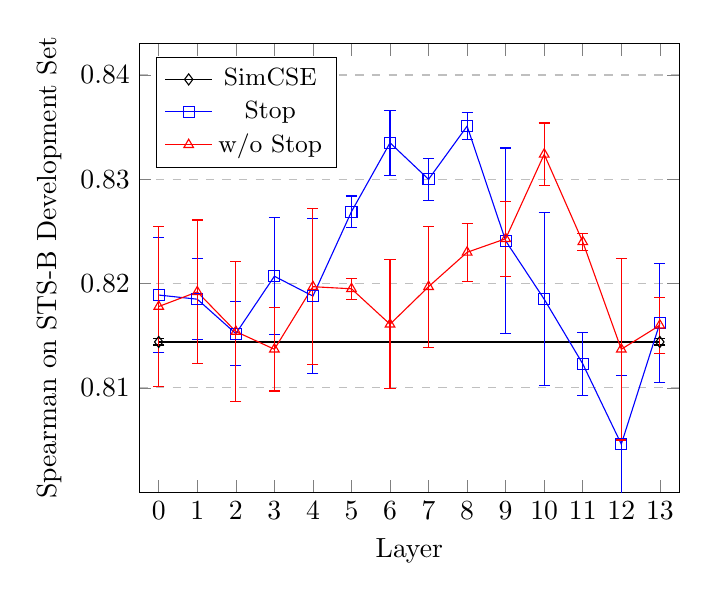
\begin{tikzpicture}
\begin{axis}[
    %title={Temperature dependence of CuSO\(_4\cdot\)5H\(_2\)O solubility},
    % width=0.8\textwidth,
    % height=0.5\textwidth,
    xlabel={Layer},
    ylabel={Spearman on STS-B Development Set},
    xmin=-0.5, xmax=13.5,
    ymin=0.8, ymax=0.843,
    xtick={0, 1, 2, 3, 4, 5, 6, 7, 8, 9, 10, 11, 12, 13}, %,11,12,13},
    ytick={0.81, 0.82, 0.83, 0.84},
    %ytick={0,0.2,0.4,0.6,0.8,1.0}, %,0.6,0.7,0.8,0.9,1.0},
    legend pos=north west,
    ymajorgrids=true,
    grid style=dashed,
]
\addplot[
    color=black,
    mark=diamond,
    error bars/.cd, y dir=both, y explicit
    ]
    coordinates {
    %(0,0.8147335170481025)(13,0.8147335170481025)
    % (0, 0.8204) +- (0, 0.0085)
    % (13, 0.8204) +- (0, 0.0085)

    %(0.8147335170481025, 0.8141535664704519)
    (0, 0.8144) +- (0, 0.00029)
    (13, 0.8144) +- (0, 0.00029)
    };
    \addlegendentry{\small SimCSE}


\addplot+[
    color=blue,
    mark=square,
    error bars/.cd, y dir=both, y explicit
    ]
    coordinates {
    % (0,0.8169731103921712)
    % (1,0.819057984441431)
    % (2,0.8166468866942407)
    % (3,0.812866365572481)
    % (4,0.8135888411587529)
    % (5,0.8249856728469834)
    % (6,0.8306805778612282)
    % (7,0.8328021611740035)
    % (8,0.8355351495654609)
    % (9,0.8306577921070178)
    % (10,0.8149157851326303)
    % (11,0.8166311607047543)
    % (12,0.8107370794093145)
    % (13,0.8081902128875393)
    (0, 0.8189) +- (0, 0.0055)
    (1, 0.8185) +- (0, 0.0039)
    (2, 0.8152) +- (0, 0.0031)
    (3, 0.8207) +- (0, 0.0056)
    (4, 0.8188) +- (0, 0.0074)
    (5, 0.8269) +- (0, 0.0015)
    (6, 0.8335) +- (0, 0.0031)
    (7, 0.8300) +- (0, 0.0020)
    (8, 0.8351) +- (0, 0.0013)
    (9, 0.8241) +- (0, 0.0089)
    (10, 0.8185) +- (0, 0.0083)
    (11, 0.8123) +- (0, 0.0030)
    (12, 0.8046) +- (0, 0.0066)
    (13, 0.8162) +- (0, 0.0057)
    };
    \addlegendentry{\small Stop}

% \addplot[
%     color=green,
%     mark=o,
%     ]
%     coordinates {
%     (0, 0.8162363070656291)
%     (1, 0.8231537007874197)
%     (2, 0.8138701196558773)
%     (3, 0.8117669082418852)
%     (4, 0.8321764667925834)
%     (5, 0.8173026949754195)
%     (6, 0.8204092789670786)
%     (7, 0.8212422830999221)
%     (8, 0.8286144945867048)
%     (9, 0.8364377846761957)
%     (10, 0.8264360518041358)
%     (11, 0.807795095724245)
%     (12, 0.829652918789954)
%     (13, 0.827621011695569)
%     };
%     \addlegendentry{\small Debug}

\addplot+[
    color=red,
    mark=triangle,
    error bars/.cd, y dir=both, y explicit
    ]
    coordinates {
% (0,0.8201958563827355)
% (1,0.824192633155200)
% (2,0.8235437910715707)
% (3,0.8178133056476282)
% (4,0.8211208445639191)
% (5,0.8207129410980774)
% (6,0.8151817237627103)
% (7,0.8173462234751712)
% (8,0.8270007756575324)
% (9,0.8254520877587794)
% (10,0.8282669249521344)
% (11,0.8251234611980554)
% (12,0.8240867548112837)
% (13,0.8147346771912509)
(0, 0.8178) +- (0, 0.0077)
(1, 0.8192) +- (0, 0.0069)
(2, 0.8154) +- (0, 0.0067)
(3, 0.8137) +- (0, 0.0040)
(4, 0.8197) +- (0, 0.0075)
(5, 0.8195) +- (0, 0.0010)
(6, 0.8161) +- (0, 0.0062)
(7, 0.8197) +- (0, 0.0058)
(8, 0.8230) +- (0, 0.0028)
(9, 0.8243) +- (0, 0.0036)
(10, 0.8324) +- (0, 0.0030)
(11, 0.8240) +- (0, 0.0008)
(12, 0.8137) +- (0, 0.0087)
(13, 0.8160) +- (0, 0.0027)
    };
    \addlegendentry{\small w/o Stop}

% \addplot[
%     dashed,
%     mark options={solid},
%     color=blue,
%     mark=square,
%     ]
%     coordinates {
%     (0,0.7632744193037913)
%     (1,0.7887974973930733)
%     (2,0.787675765303225)
%     (3,0.7861854902547428)
%     (4,0.7574942818680372)
%     (5,0.7829649115225943)
%     (6,0.7976033379818234)
%     (7,0.8124762681613964)
%     (8,0.8102590246403415)
%     (9,0.7590563327667009)
%     (10,0.7379011420294991)
%     (11,0.6796433898476625)
%     (12,0.6775176769243549)
%     (13,0.691473581560862)
%     };
%     \addlegendentry{\small Stop*}

% \addplot[
%     dashed,
%     mark options={solid},
%     color=red,
%     mark=triangle,
%     ]
%     coordinates {
%     (0,0.7585592528117979)
%     (1,0.7991558675216115)
%     (2,0.7892084923382617)
%     (3,0.8044671131751203)
%     (4,0.7909274995641637)
%     (5,0.8056261066829183)
%     (6,0.7888484920901417)
%     (7,0.79693944606518)
%     (8,0.7913087589103663)
%     (9,0.7845707685012719)
%     (10,0.8120686878093089)
%     (11,0.8226423410043743)
%     (12,0.7952155961226167)
%     (13,0.7878095073882856)
    
%     };
%     \addlegendentry{\small w/o Stop*}

\end{axis}
\end{tikzpicture}
}
\caption{Dropout}
\label{fig:simcsetop}
\end{subfigure}
%\begin{figure}[ht]
\begin{subfigure}{.49\columnwidth}
\resizebox{1.0\columnwidth}{!}{%
\centering
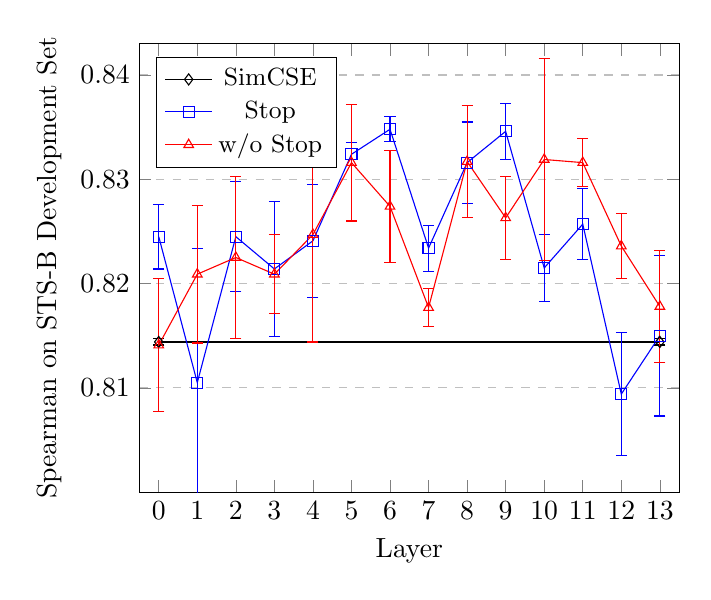
\begin{tikzpicture}
\begin{axis}[
    %title={Temperature dependence of CuSO\(_4\cdot\)5H\(_2\)O solubility},
    % width=0.8\textwidth,
    % height=0.5\textwidth,
    xlabel={Layer},
    ylabel={Spearman on STS-B Development Set},
    xmin=-0.5, xmax=13.5,
    ymin=0.8, ymax=0.843,
    xtick={0, 1, 2, 3, 4, 5, 6, 7, 8, 9, 10, 11, 12, 13}, %,11,12,13},
    ytick={0.81, 0.82, 0.83, 0.84},
    %ytick={0,0.2,0.4,0.6,0.8,1.0}, %,0.6,0.7,0.8,0.9,1.0},
    legend pos=north west,
    ymajorgrids=true,
    grid style=dashed,
]
\addplot[
    color=black,
    mark=diamond,
    error bars/.cd, y dir=both, y explicit
    ]
    coordinates {
    % (0,0.8147335170481025)(13,0.8147335170481025)

    %(0.8147335170481025, 0.8141535664704519)
    % (0.8144 +- 0.00029)
    %(0, 0.8204) +- (0, 0.0085)
    %(13, 0.8204) +- (0, 0.0085)
    (0, 0.8144) +- (0, 0.00029)
    (13, 0.8144) +- (0, 0.00029)
    };
    \addlegendentry{\small SimCSE}


\addplot[
    color=blue,
    mark=square,
    error bars/.cd, y dir=both, y explicit
    ]
    coordinates {
    % (0, 0.8270687529988076)
    % (1, 0.7936702516411613)
    % (2, 0.8181233592421068)
    % (3, 0.8196901076529048)
    % (4, 0.8167808227296128)
    % (5, 0.8331369959243518)
    % (6, 0.8351675738363259)
    % (7, 0.820671206193868)
    % (8, 0.8358895423054524)
    % (9, 0.837599696509039)
    % (10, 0.8201366969286754)
    % (11, 0.8286827419647032)
    % (12, 0.801244753302954)
    % (13, 0.811439068879559)
(0, 0.8245) +- (0, 0.0031)
(1, 0.8105) +- (0, 0.0129)
(2, 0.8245) +- (0, 0.0053)
(3, 0.8214) +- (0, 0.0065)
(4, 0.8241) +- (0, 0.0054)
(5, 0.8324) +- (0, 0.0011)
(6, 0.8348) +- (0, 0.0012)
(7, 0.8234) +- (0, 0.0022)
(8, 0.8316) +- (0, 0.0039)
(9, 0.8346) +- (0, 0.0027)
(10, 0.8215) +- (0, 0.0032)
(11, 0.8257) +- (0, 0.0034)
(12, 0.8094) +- (0, 0.0059)
(13, 0.8150) +- (0, 0.0077)
    };
    \addlegendentry{\small Stop}

\addplot[
    color=red,
    mark=triangle,
    error bars/.cd, y dir=both, y explicit
    ]
    coordinates {
% (0, 0.8090408092173771)
% (1, 0.8190863036943639)
% (2, 0.8244007959529946)
% (3, 0.8196361004982442)
% (4, 0.8128809712873017)
% (5, 0.8276497839573925)
% (6, 0.8317617636597858)
% (7, 0.816198222683944)
% (8, 0.8371667691643927)
% (9, 0.8268938724043733)
% (10, 0.8186735944967859)
% (11, 0.8300833728232869)
% (12, 0.8279872913074475)
% (13, 0.81019290893641)
(0, 0.8141) +- (0, 0.0064)
(1, 0.8209) +- (0, 0.0066)
(2, 0.8225) +- (0, 0.0078)
(3, 0.8209) +- (0, 0.0038)
(4, 0.8247) +- (0, 0.0103)
(5, 0.8316) +- (0, 0.0056)
(6, 0.8274) +- (0, 0.0054)
(7, 0.8177) +- (0, 0.0018)
(8, 0.8317) +- (0, 0.0054)
(9, 0.8263) +- (0, 0.0040)
(10, 0.8319) +- (0, 0.0097)
(11, 0.8316) +- (0, 0.0023)
(12, 0.8236) +- (0, 0.0031)
(13, 0.8178) +- (0, 0.0054)
    };
    \addlegendentry{\small w/o Stop}

\end{axis}
\end{tikzpicture}
}
%\vspace{-.2in}
\caption{PCA}
\label{fig:simcsetop-pca1-N}
%\vspace{-0.5cm}
\end{subfigure}
% \caption{SimCSE vs.\ Deep Augmentation with and without stop-gradient. ``Stop'': stop-gradient. Deep Augmentation outperforms SimCSE.\vspace{-.1in}}
\vspace{-.1in}
\caption{SimCSE vs.\ Deep Augmentation with (a) Dropout or (b) PCA, with and without stop-gradient. ``Stop'': stop-gradient. Deep Augmentation outperforms SimCSE.}
%\label{fig:simcsetop}
%\vspace{-0.5cm}
\end{figure}


% \begin{figure}[ht]
% \centering
% \begin{tikzpicture}
% \begin{axis}[
%     %title={Temperature dependence of CuSO\(_4\cdot\)5H\(_2\)O solubility},
%     % width=0.8\textwidth,
%     % height=0.5\textwidth,
%     xlabel={Layer},
%     ylabel={Spearman on STS-B Development Set},
%     xmin=-0.5, xmax=13.5,
%     ymin=0.8, ymax=0.843,
%     xtick={0, 1, 2, 3, 4, 5, 6, 7, 8, 9, 10, 11, 12, 13}, %,11,12,13},
%     ytick={0.81, 0.82, 0.83, 0.84},
%     %ytick={0,0.2,0.4,0.6,0.8,1.0}, %,0.6,0.7,0.8,0.9,1.0},
%     legend pos=north west,
%     ymajorgrids=true,
%     grid style=dashed,
% ]
% \addplot[
%     color=black,
%     %mark=diamond,
%     ]
%     coordinates {
%     (0,0.8147335170481025)(13,0.8147335170481025)
%     };
%     \addlegendentry{\small SimCSE}


% \addplot[
%     color=blue,
%     mark=square,
%     ]
%     coordinates {
%     (0, 0.8270687529988076)
%     (1, 0.7936702516411613)
%     (2, 0.8181233592421068)
%     (3, 0.8196901076529048)
%     (4, 0.8167808227296128)
%     (5, 0.8331369959243518)
%     (6, 0.8351675738363259)
%     (7, 0.820671206193868)
%     (8, 0.8358895423054524)
%     (9, 0.837599696509039)
%     (10, 0.8201366969286754)
%     (11, 0.8286827419647032)
%     (12, 0.801244753302954)
%     (13, 0.811439068879559)
%     };
%     \addlegendentry{\small Stop}

% \addplot[
%     color=red,
%     mark=triangle,
%     ]
%     coordinates {
%     (0, 0.8090408092173771)
%     (1, 0.8190863036943639)
%     (2, 0.8244007959529946)
%     (3, 0.8196361004982442)
%     (4, 0.8128809712873017)
%     (5, 0.8276497839573925)
%     (6, 0.8317617636597858)
%     (7, 0.816198222683944)
%     (8, 0.8371667691643927)
%     (9, 0.8268938724043733)
%     (10, 0.8186735944967859)
%     (11, 0.8300833728232869)
%     (12, 0.8279872913074475)
%     (13, 0.81019290893641)
%     };
%     \addlegendentry{\small w/o Stop}

% \end{axis}
% \end{tikzpicture}
% \vspace{-.2in}
% \caption{SimCSE vs.\ Deep Augmentation PCA with and without stop-gradient. Deep Augmentation outperforms SimCSE.\vspace{-.1in}}
% \label{fig:simcsetop-pca1-N}
% %\vspace{-0.5cm}
% \end{figure}



%\subsubsection{Deep Augmentation and Masked Language Modeling}

\textbf{Deep Augmentation and Masked Language Modeling (MLM).}
We assess Deep Augmentation alongside MLM's original data augmentation techniques, following SimCSE's experimental setup in Figure \ref{fig:simcse-mlm-N}. Despite SimCSE's performance optimization across dropout rates (0\%, 1\%, 5\%, 10\%, 15\%, 20\%), it underperforms. Integrating Deep Augmentation with a standard 50\% dropout rate boosts performance, highlighting the effectiveness of layer-specific augmentation. This combination enhances training robustness, reduces development set dependence, and supports simultaneous Deep Augmentation and MLM training. On STS tasks, the best Deep Augmentation setups outperform SimCSE's highest Spearman's correlation scores: $74.32$ vs.\ $69.31$. In the Appendix, we show that even for MLM without contrastive learning, Deep Augmentation markedly improves performance, and there stop-gradient's effect is less pronounced.

% In this section, we examine the efficacy of Deep Augmentation when integrated with the original data augmentation strategies employed in Masked Language Modeling (MLM). Adhering to the experimental protocol established in SimCSE, we obtained the results depicted in Figure \ref{fig:simcse-mlm-N}. SimCSE, even after optimization across a range of dropout rates (0\%, 1\%, 5\%, 10\%, 15\%, 20\%, denoted as 'SimCSE*'), exhibits suboptimal performance. However, the integration of Deep Augmentation, utilizing an unadjusted 50\% dropout rate, resulted in a marked enhancement in performance. This underscores the importance of targeted layer-specific augmentation, effectively amalgamating the invariances fostered by MLM with the higher-layer invariances induced by Deep Augmentation. This synergy potentially facilitates more robust training, diminishes the reliance on a development set, and allows for the concurrent training of Deep Augmentation and MLM from the outset. These results generalize to the STS tasks, and the optimally performing configurations of Deep Augmentation, as evaluated on the development set, achieved an average Spearman's correlation of $74.32$ on the STS tasks. This performance surpasses that of the best configurations of SimCSE on the same set, which attained a Spearman's correlation of $69.31$. In the Appendix, we present additional results obtained using MLM and Deep Augmentation, but without employing contrastive loss. Notably, Deep Augmentation significantly enhances performance, while the application of stop-gradient exhibits a comparatively minor impact.


\begin{figure}[ht]
\centering
\resizebox{0.33\columnwidth}{!}{%
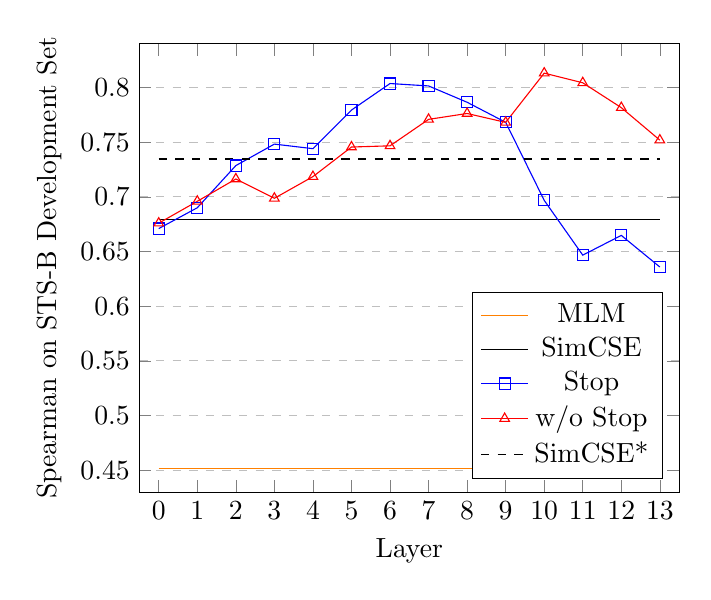
\begin{tikzpicture}
\begin{axis}[
    %title={Temperature dependence of CuSO\(_4\cdot\)5H\(_2\)O solubility},
    % width=0.8\textwidth,
    % height=0.5\textwidth,
    xlabel={Layer},
    ylabel={Spearman on STS-B Development Set},
    xmin=-0.5, xmax=13.5,
    ymin=0.43, ymax=0.84,
    xtick={0, 1, 2, 3, 4, 5, 6, 7, 8, 9, 10, 11, 12, 13}, %,11,12,13},
    ytick={0.45, 0.50, 0.55, 0.6, 0.65,0.7,0.75,0.8},
    %ytick={0,0.2,0.4,0.6,0.8,1.0}, %,0.6,0.7,0.8,0.9,1.0},
    legend pos=south east,
    ymajorgrids=true,
    grid style=dashed,
]
\addplot[
    color=orange,
    %mark=o,
    ]
    coordinates {
    (0,0.4517664038939373)(1,0.4517664038939373)(2,0.4517664038939373)(3,0.4517664038939373)(4,0.4517664038939373)(5,0.4517664038939373)(6,0.4517664038939373)(7,0.4517664038939373)(8,0.4517664038939373)(9,0.4517664038939373)(10,0.4517664038939373)(11,0.4517664038939373)(12,0.4517664038939373)(13,0.4517664038939373)
    };
    \addlegendentry{MLM}


\addplot[
    color=black,
    %mark=diamond,
    ]
    coordinates {
    (0,0.6794310092039192)(1,0.6794310092039192)(2,0.6794310092039192)(3,0.6794310092039192)(4,0.6794310092039192)(5,0.6794310092039192)(6,0.6794310092039192)(7,0.6794310092039192)(8,0.6794310092039192)(9,0.6794310092039192)(10,0.6794310092039192)(11,0.6794310092039192)(12,0.6794310092039192)(13,0.6794310092039192)
    };
    \addlegendentry{SimCSE}

\addplot[
    color=blue,
    mark=square,
    ]
    coordinates {
    (0,0.6710064393405828)
    (1,0.6900287205210686)
    (2,0.72860088650924)
    (3,0.7482461022310182)
    (4,0.744069669412655)
    (5,0.7793759991035901)
    (6,0.8036405432104125)
    (7,0.8014485968598176)
    (8,0.786510552756363)
    (9,0.7681913230485004)
    (10,0.6968147347082932)
    (11,0.6467046002123376)
    (12,0.6647613549651601)
    (13,0.6358397869890808)
    };
    \addlegendentry{Stop}

\addplot[
    color=red,
    mark=triangle,
    ]
    coordinates {
    (0,0.6759434516400763)
    (1,0.6959413906899954)
    (2,0.7163384047480618)
    (3,0.698689917495372)
    (4,0.7185099809778556)
    (5,0.7455810616864732)
    (6,0.7466678117727463)
    (7,0.7708708391301566)
    (8,0.7762493303816139)
    (9,0.7681124689016257)
    (10,0.8131356618542991)
    (11,0.8043112767687819)
    (12,0.7815920242604428)
    (13,0.7518832279573735)
    };
    \addlegendentry{w/o Stop}

\addplot[
    dashed,
    mark options={solid},
    color=black,
    %mark=diamond,
    ]
    coordinates {
    (0,0.734639170030387)
    (1,0.734639170030387)
    (2,0.734639170030387)
    (3,0.734639170030387)
    (4,0.734639170030387)
    (5,0.734639170030387)
    (6,0.734639170030387)
    (7,0.734639170030387)
    (8,0.734639170030387)
    (9,0.734639170030387)
    (10,0.734639170030387)
    (11,0.734639170030387)
    (12,0.734639170030387)
    (13,0.734639170030387)
    };
    \addlegendentry{SimCSE*}


\end{axis}
\end{tikzpicture}
}
\vspace{-.1in}
\caption{SimCSE vs.\ Deep Augmentation with and without stop-gradient, both with MLM. ``Stop'': stop-gradient. *: includes hyperparameter search over dropout rates.}
\label{fig:simcse-mlm-N}
%\vspace{-0.5cm}
\end{figure}

%\subsubsection{Supervised Learning}

%Is there a difference between contrastive versus supervised setting?

\textbf{Supervised Learning.}
This section evaluates Deep Augmentation in supervised learning and compares it to contrastive learning outcomes. Deep Augmentation results with dropout and PCA are in Figures \ref{fig:simcse-supervised-dropout-N} and \ref{fig:simcse-supervised-pca-N}, resp. In supervised learning, Deep Augmentation reduces performance, especially in higher layers, contrasting with the positive effects in contrastive learning.

% In this section we explore the application of Deep Augmentation to supervised learning to see how it compares to contrastive learning. See Figures \ref{fig:simcse-supervised-dropout-N} and \ref{fig:simcse-supervised-pca-N} for results with Deep Augmentation with dropout and PCA respectively. Note that performance is significantly reduced when applying Deep Augmentation to supervised learning.
\begin{figure}[ht]
\centering
\begin{subfigure}{.33\columnwidth}
\centering
\resizebox{1.0\columnwidth}{!}{%
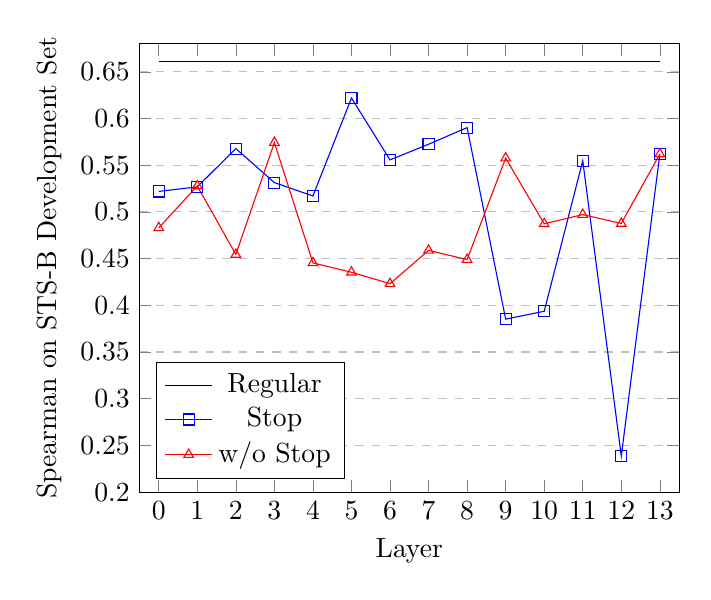
\begin{tikzpicture}
\begin{axis}[
    %title={Temperature dependence of CuSO\(_4\cdot\)5H\(_2\)O solubility},
    % width=0.8\textwidth,
    % height=0.5\textwidth,
    xlabel={Layer},
    ylabel={Spearman on STS-B Development Set},
    xmin=-0.5, xmax=13.5,
    ymin=0.20, ymax=0.68,
    xtick={0, 1, 2, 3, 4, 5, 6, 7, 8, 9, 10, 11, 12, 13}, %,11,12,13},
    ytick={0.10, 0.15, 0.20, 0.25, 0.30, 0.35, 0.40, 0.45, 0.50, 0.55, 0.6, 0.65,0.7,0.75,0.8},
    %ytick={0,0.2,0.4,0.6,0.8,1.0}, %,0.6,0.7,0.8,0.9,1.0},
    legend pos=south west,
    ymajorgrids=true,
    grid style=dashed,
]
\addplot[
    color=black,
    %mark=o,
    ]
    coordinates {
    (0, 0.6609508549999146)(13, 0.6609508549999146)
    };
    \addlegendentry{Regular}

\addplot[
    %dashed,
    mark options={solid},
    color=blue,
    mark=square,
    ]
    coordinates {
    (0, 0.5219260897715743)%+-(0,0.0)
    (1, 0.5268079915513444)%+-(0,0.0)
    (2, 0.5677703226214103)%+-(0,0.0)
    (3, 0.531370576758617)%+-(0,0.0)
    (4, 0.5170367798180009)%+-(0,0.0)
    (5, 0.6219622891281111)%+-(0,0.0)
    (6, 0.5556737117035734)%+-(0,0.0)
    (7, 0.5724294775204014)%+-(0,0.0)
    (8, 0.5902619322906782)%+-(0,0.0)
    (9, 0.3851943765346928)%+-(0,0.0)
    (10, 0.39359754550573056)%+-(0,0.0)
    (11, 0.554742162481777)%+-(0,0.0)
    (12, 0.23861411013833497)%+-(0,0.0)
    (13, 0.5619841311338378)%+-(0,0.0)
    
    };
    \addlegendentry{Stop}


\addplot[
    %dashed,
    mark options={solid},
    color=red,
    mark=triangle,
    ]
    coordinates {

    (0, 0.48291278417278466)%+-(0,0.0)
    (1, 0.5276996113119281)%+-(0,0.0)
    (2, 0.4544394223462644)%+-(0,0.0)
    (3, 0.574207388837405)%+-(0,0.0)
    (4, 0.4453952791190298)%+-(0,0.0)
    (5, 0.4353779987307919)%+-(0,0.0)
    (6, 0.42315742116431493)%+-(0,0.0)
    (7, 0.45875674523048504)%+-(0,0.0)
    (8, 0.4489637121416536)%+-(0,0.0)
    (9, 0.5575690428044277)%+-(0,0.0)
    (10, 0.4872831279570815)%+-(0,0.0)
    (11, 0.49710027082614716)%+-(0,0.0)
    (12, 0.4876110667825768)%+-(0,0.0)
    (13, 0.5619841311338378)%+-(0,0.0)
    };
    \addlegendentry{w/o Stop}

\end{axis}
\end{tikzpicture}
}
\vspace{-.2in}
\caption{Dropout} % *: includes hyperparameter search over dropout rates.\vspace{-.2in}}
\label{fig:simcse-supervised-dropout-N}
%\vspace{-0.5cm}
\end{subfigure}
\hspace{.2in}
\begin{subfigure}{.33\columnwidth}
\centering
\resizebox{1.0\columnwidth}{!}{%
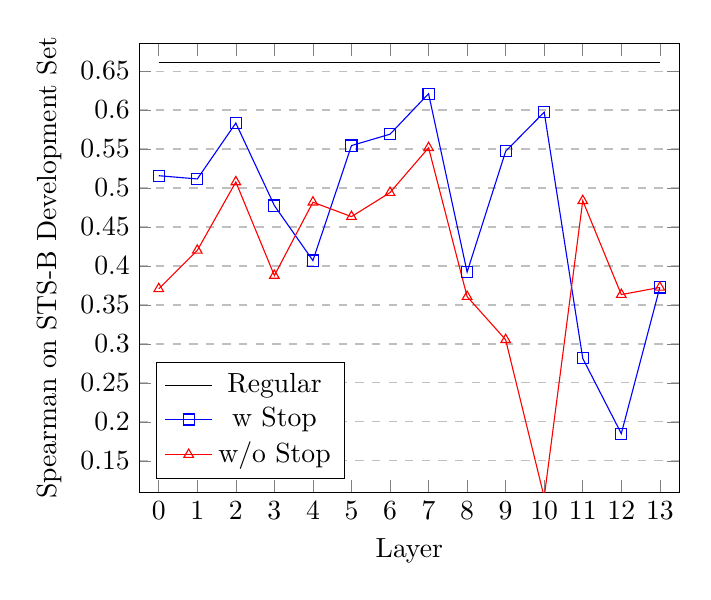
\begin{tikzpicture}
\begin{axis}[
    %title={Temperature dependence of CuSO\(_4\cdot\)5H\(_2\)O solubility},
    % width=0.8\textwidth,
    % height=0.5\textwidth,
    xlabel={Layer},
    ylabel={Spearman on STS-B Development Set},
    xmin=-0.5, xmax=13.5,
    ymin=0.11, ymax=0.685,
    xtick={0, 1, 2, 3, 4, 5, 6, 7, 8, 9, 10, 11, 12, 13}, %,11,12,13},
    ytick={0.10, 0.15, 0.20, 0.25, 0.30, 0.35, 0.40, 0.45, 0.50, 0.55, 0.6, 0.65,0.7,0.75,0.8},
    %ytick={0,0.2,0.4,0.6,0.8,1.0}, %,0.6,0.7,0.8,0.9,1.0},
    legend pos=south west,
    ymajorgrids=true,
    grid style=dashed,
]
\addplot[
    color=black,
    %mark=o,
    ]
    coordinates {
    %(0, 0.5679517679024151)(13, 0.5679517679024151)
    (0, 0.6609508549999146)(13, 0.6609508549999146)
    };
    \addlegendentry{Regular}

\addplot[
    %dashed,
    mark options={solid},
    color=blue,
    mark=square,
    ]
    coordinates {
    (0, 0.5157765411796097)+-(0,0.07676785741471635)
    (1, 0.5116403741826738)+-(0,0.011904671403655212)
    (2, 0.5832869358356717)+-(0,0.024370201425615117)
    (3, 0.47746536354055386)+-(0,0.09192107546270112)
    (4, 0.40695369752637195)+-(0,0.2575299971623067)
    (5, 0.5544333946539806)+-(0,0.04132307836495922)
    (6, 0.5690227262493507)+-(0,0.04823427871500068)
    (7, 0.6209589496473172)+-(0,0.043212086990046146)
    (8, 0.3922407110688484)+-(0,0.3188615677210013)
    (9, 0.5470962444837713)+-(0,0.024176251902270556)
    (10, 0.5972832912994855)+-(0,0.028142609184769896)
    (11, 0.2814614184901056)+-(0,0.20089456241770634)
    (12, 0.18499741087423463)+-(0,0.19021642475550865)
    (13, 0.3725057064892073)+-(0,0.23412157075552859)
    
    };
    \addlegendentry{w Stop}

\addplot[
    %dashed,
    mark options={solid},
    color=red,
    mark=triangle,
    ]
    coordinates {
    (0, 0.37071019283275275)+-(0,0.2579976631080303)
    (1, 0.41999558173685075)+-(0,0.13150689184153552)
    (2, 0.5077316332346334)+-(0,0.05947326006435447)
    (3, 0.38775168927967113)+-(0,0.10686510831471742)
    (4, 0.4818139607994012)+-(0,0.0799504493603165)
    (5, 0.46330676662702225)+-(0,0.04682410459143695)
    (6, 0.4941405862746053)+-(0,0.06816138730916133)
    (7, 0.5516334936144659)+-(0,0.02781172403853759)
    (8, 0.36074319208601485)+-(0,0.1954752541706238)
    (9, 0.30535412122943645)+-(0,0.2597180492817242)
    (10, 0.10352186514540335)+-(0,0.22268575833452645)
    (11, 0.483630973865764)+-(0,0.09861445496828604)
    (12, 0.36331341360087127)+-(0,0.20690779050394423)
    (13, 0.3725057064892073)+-(0,0.23412157075552859)
    
    };
    \addlegendentry{w/o Stop}

% \addplot[
%     %dashed,
%     mark options={solid},
%     color=cyan,
%     mark=square,
%     ]
%     coordinates {
%     (0, 0.570221291955367)+-(0,0.04750633293870542)
%     (1, 0.546144549946633)+-(0,0.044720998403206216)
%     (2, 0.5246587163158383)+-(0,0.09418562928018405)
%     (3, 0.42129268256845154)+-(0,0.13837228720479292)
%     (4, 0.5877488754048478)+-(0,0.022382265762949553)
%     (5, 0.6042620895785867)+-(0,0.015342652201262257)
%     (6, 0.61141769749417)+-(0,0.007173348769554877)
%     (7, 0.5790314783039249)+-(0,0.028593303192443006)
%     (8, 0.4134020681559519)+-(0,0.29170979993796886)
%     (9, 0.433077312425113)+-(0,0.21416959259506446)
%     (10, 0.41686309618748424)+-(0,0.14974262267812044)
%     (11, 0.3007699727293889)+-(0,0.27086502032371496)
%     (12, 0.4591478818412811)+-(0,0.0695072097899404)
%     (13, 0.3725057064892073)+-(0,0.23412157075552859)
%     };
%     \addlegendentry{6 w Stop}


% \addplot[
%     %dashed,
%     mark options={solid},
%     color=magenta,
%     mark=triangle,
%     ]
%     coordinates {

%     (0, 0.3807432826801573)+-(0,0.268763403389643)
%     (1, 0.5653821998297167)+-(0,0.01694064135112207)
%     (2, 0.5483218383415199)+-(0,0.01198665579663902)
%     (3, 0.47636712735390035)+-(0,0.09858374805431447)
%     (4, 0.5654947533703548)+-(0,0.036789497391976976)
%     (5, 0.514446945785613)+-(0,0.0350801990024105)
%     (6, 0.5745960957626678)+-(0,0.0253454761925798)
%     (7, 0.4174499867650307)+-(0,0.13339998426276178)
%     (8, 0.35215777970128054)+-(0,0.12791413696752438)
%     (9, 0.37414643408868803)+-(0,0.2643474402547746)
%     (10, 0.5883293572107041)+-(0,0.03869618095470662)
%     (11, 0.5029776999834151)+-(0,0.055180552501187856)
%     (12, 0.35204846209932045)+-(0,0.18912582819667895)
%     (13, 0.3725057064892073)+-(0,0.2341215707555286)
%     };
%     \addlegendentry{6 w/o Stop}

\end{axis}
\end{tikzpicture}
}
\vspace{-.2in}
\caption{PCA} % *: includes hyperparameter search over dropout rates.\vspace{-.2in}}
\label{fig:simcse-supervised-pca-N}
%\vspace{-0.5cm}
\end{subfigure}
%\begin{figure}[ht]
\vspace{-.1in}
\caption{Supervised only. Deep Augmentation with (a) Dropout (across dropout rates .5, .25, .125) and (b) PCA, with and witout stop-gradient, on STS-B.} % *: includes hyperparameter search over dropout rates.\vspace{-.2in}}
\label{fig:simcse-supervised-N}
\vspace{-.2in}
\end{figure}

\subsection{Vision}
\label{sec:vision}

Our primary results focus on the CIFAR-100 dataset, with corresponding outcomes for CIFAR-10 in the Appendix. For ImageNet100, we applied the optimal configuration from CIFAR, involving layer-targeted dropout and stop-gradient at the fourth layer.

%No additional hyperparameter optimization or ablation studies were done on ImageNet100, primarily due to the constraints imposed by computational resources. 

%\subsubsection{Architecture}

\textbf{Architecture.} 
We use ResNet18 (Appendix \ref{appendix:resnetarch}, Table \ref{table:resnet18-N}). In contrast to transformers and GNNs, ResNet exhibits less regularity. Specifically, it comprises convolutional layers at the beginning, followed by a fully connected layer, with average pooling interposed, and the layers vary in dimensions. 

%For more details, please see the Appendix.

%While an in-depth exploration of the specific architecture and its dimensions is beyond the scope of this main text, a more detailed discussion is provided in the Appendix.

% \begin{table}[ht] % [H]
% \caption{Configuration of ResNet18 on CIFAR}
% \centering
% \begin{tabular}{ |p{0.7cm}||p{2.4cm}|p{2.8cm}|  }
%  \hline
%  \multicolumn{3}{|c|}{ResNet18 on CIFAR} \\
%  \hline
%  Layer & Type & \#Neurons  \\
%  \hline
%  -1    & Input Data        & $32^2\times3=3072$      \\
%  0     & Conv(k=3, s=1)    & $32^2\times64=65536$    \\
%  1     & Conv(k=3, s=2)    & $32^2\times64=65536$    \\
%  2     & Conv(k=3, s=2)    & $16^2\times128=32768$   \\
%  3     & Conv(k=3, s=2)    & $8^2\times256=16384$    \\
%  4     & Conv(k=3, s=2)    & $4^2\times512=8192$     \\
%  5     & Avgpool           & $512$                  \\
%  6     & MLP               & $128$                  \\
%  \hline
% \end{tabular}
% \label{table:resnet18-N}
% \end{table}

%\subsubsection{Dropout is not a Sufficient Augmentation}

\textbf{Dropout is not a Sufficient Augmentation.} 
In our experiments, using only dropout for augmentation, without other data augmentations, did not produce competitive outcomes. Thus, for vision, we combined ``deep'' augmentations (including dropout) with data augmentations. Future research could explore if using a development set for early stopping and hyperparameter selection enables adaptation of pre-trained vision models to new image data using dropout alone, similar to methods in SimCSE and Section \ref{sec:sentence-embeddings}.

% In our initial experiments, the application of dropout as the sole form of augmentation, devoid of additional data augmentations, failed to yield competitive results. Consequently, in the vision-related segment of this study, we incorporate ``deep'' augmentations (including dropout) alongside data augmentations. However, it remains a prospective area for future research to investigate whether employing a development set for early stopping and selecting hyper-parameters, might facilitate the use of dropout without other data augmentations to effectively adapt a pre-trained vision model to novel image data, akin to the approach utilized in SimCSE and Section \ref{sec:sentence-embeddings}.
 

%\subsubsection{Data Augmentation and Targeted Dropout}

\textbf{Data Augmentation and Targeted Dropout.}
Our results show that general dropout reduces contrastive learning effectiveness. However, layer-specific application of dropout shows varying performance impacts across layers (Figure \ref{fig:CIFAR100-CIFAR100-drop-all-vs-layer-N}). Notably, a uniform 50\% dropout rate significantly hinders performance, whereas targeting 50\% dropout at certain layers results in a much smaller decrease in performance.

% Our findings indicate that dropout diminishes the efficacy of contrastive learning. However, when dropout is applied in a layer-targeted manner, there is variation in performance across layers (Figure \ref{fig:CIFAR100-CIFAR100-drop-all-vs-layer-N}). Specifically, a uniform dropout rate of 50\% substantially degrades performance. In contrast, 50\% dropout targeted at specific layers yields a markedly less pronounced performance decline.


\begin{figure}[ht] % [ht]
\centering
\resizebox{0.33\columnwidth}{!}{%
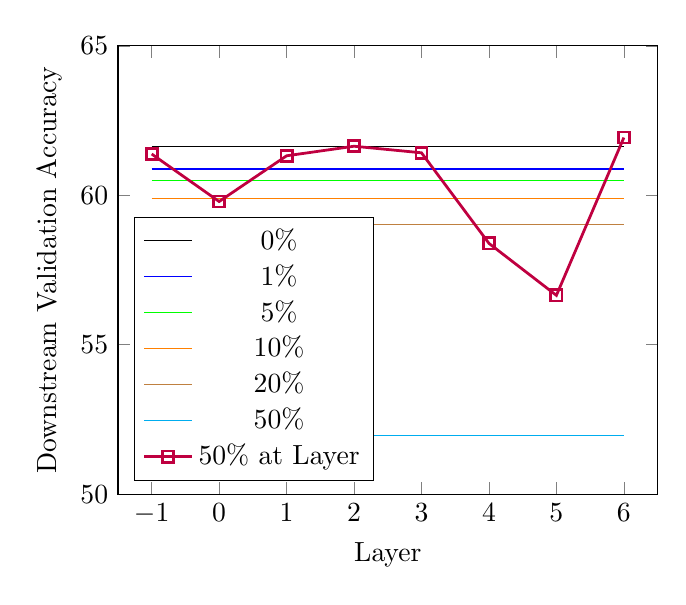
\begin{tikzpicture}
\begin{axis}[
    %title={Temperature dependence of CuSO\(_4\cdot\)5H\(_2\)O solubility},
    % width=0.8\textwidth,
    % height=0.5\textwidth,
    xlabel={Layer},
    ylabel={Downstream Validation Accuracy},
    xmin=-1.5, xmax=6.5,
    ymin=57, ymax=65,
    xtick={-1,0,1,2,3,4,5,6,7}, %,11,12,13},
    ymin=50, ymax=65,
    %ytick={51,52,53,54,55,56,57,58,59,60,61,62,63,64,65},
    ytick={50, 55, 60, 65}, % ,52,53,54,55,56,57,58,59,60,61,62,63,64,65},
    %ytick={0,0.2,0.4,0.6,0.8,1.0}, %,0.6,0.7,0.8,0.9,1.0},
    legend pos=south west,
    %ymajorgrids=true,
    %grid style=dashed,
]
\addplot[
    %dashed,
    mark options={solid},
    color=black,
    %mark=diamond,
    ]
    coordinates {
    % (300,62.14999771118164)(600,63.15999984741211)(900,62.91999816894531)(1200,62.29999923706055)(1500,61.93000030517578)
    (-1,61.64)
    (0,61.64)
    (1,61.64)
    (2,61.64)
    (3,61.64)
    (4,61.64)
    (5,61.64)
    (6,61.64)
    };
    \addlegendentry{0\%}
\addplot[
    %dashed,
    mark options={solid},
    color=blue,
    %mark=pentagon,
    ]
    coordinates {
    (-1, 60.87999725341797)
    (0, 60.87999725341797) 
    (1, 60.87999725341797)
    (2, 60.87999725341797)
    (3, 60.87999725341797)
    (4, 60.87999725341797)
    (5, 60.87999725341797)
    (6, 60.87999725341797)
    };
    \addlegendentry{1\%}
\addplot[
    %dashed,
    mark options={solid},
    color=green,
    %mark=triangle,
    ]
    coordinates {
    (-1, 60.5)
    (0, 60.5)
    (1, 60.5)
    (2, 60.5)
    (3, 60.5)
    (4, 60.5)
    (5, 60.5)
    (6, 60.5)
    };
    \addlegendentry{5\%}
\addplot[
    %dashed,
    mark options={solid},
    color=orange,
    %mark=o,
    ]
    coordinates {
    (-1, 59.87999725341797)
    (0, 59.87999725341797)
    (1, 59.87999725341797)
    (2, 59.87999725341797)
    (3, 59.87999725341797)
    (4, 59.87999725341797)
    (5, 59.87999725341797)
    (6, 59.87999725341797)
    };
    \addlegendentry{10\%}
\addplot[
    %dashed,
    mark options={solid},
    color=brown,
    %mark=diamond,
    ]
    coordinates {
    (-1, 59.0099983215332)
    (0, 59.0099983215332)
    (1, 59.0099983215332)
    (2, 59.0099983215332)
    (3, 59.0099983215332)
    (4, 59.0099983215332)
    (5, 59.0099983215332)
    (6, 59.0099983215332)
    };
    \addlegendentry{20\%}
\addplot[
    %dashed,
    mark options={solid},
    color=cyan,
    %mark=square,
    ]
    coordinates {
    (-1, 51.96999740600586)
    (0, 51.96999740600586)
    (1, 51.96999740600586)
    (2, 51.96999740600586)
    (3, 51.96999740600586)
    (4, 51.96999740600586)
    (5, 51.96999740600586)
    (6, 51.96999740600586)
    };
    \addlegendentry{50\%}

\addplot[
    % dashed,
    % mark options={solid},
    %very thick,
    line width=1pt,
    color=purple,
    mark=square,
    ]
    coordinates {
    (-1, 61.37999725341797)
    (0, 59.78999710083008)
    (1, 61.31999969482422)
    (2, 61.63999938964844)
    (3, 61.41999816894531)
    (4, 58.38999938964844)
    (5, 56.64999771118164)
    (6, 61.93000030517578) 
    };
    \addlegendentry{50\% at Layer}


\end{axis}
\end{tikzpicture}
}
\vspace{-.1in}
%\caption{Continue CIFAR100-CIFAR100}
\caption{Comparing dropout rates at all layers versus 50\% dropout rate targeted at a specific layer. For ratio of dropped to total nodes when targeting a layer, see Appendix \ref{appenxix:ratio}; there is no trend.\vspace{-.1in}}
\label{fig:CIFAR100-CIFAR100-drop-all-vs-layer-N}
%\vspace{-0.5cm}
\end{figure}

%\subsubsection{Stop-gradient \& Partial Batch}

\textbf{Augmentation, Layer, and Stop-Gradient.}
Now we apply Deep Augmentation with dropout (Figure \ref{fig:CIFAR100-CIFAR100-stop-vs-not-N}), with and without stop-gradient. Deep Augmentation with dropout and stop-gradient demonstrate significant performance improvements, particularly for layers 4 and 6; however, not using the stop-gradient did not achieve performance comparable to using stop-gradient. A small tuning of dropout rate yielded the results in Table \ref{table:keyCV} (Appendix \ref{appendix:vision}). We also evaluate Deep Augmentation with PCA augmentation, removing the largest and the sixth largest principal component. Removing the sixth largest yields superior performance (results with and without stop-gradient in Figure \ref{fig:CIFAR100-CIFAR100-stop-vs-not-pca-6-N}). For the largest, see the Appendix. Similar to dropout, stop-gradient consistently enhances performance, especially in higher layers.

%We also evaluate Deep Augmentation with PCA augmentation, with $p=1$ and $p=6$, corresponding to removing the largest and the sixth largest principal components, resp. The results indicate that $p=6$ yields superior performance compared to $p=1$. Figure \ref{fig:CIFAR100-CIFAR100-stop-vs-not-pca-6-N} presents results for $p=6$ with and without stop-gradient. For $p=1$, see the Appendix. Similar to dropout, stop-gradient consistently enhances performance, especially in higher layers.



% The results, depicted in Figure \ref{fig:CIFAR100-CIFAR100-stop-vs-not-N}, demonstrate significant performance improvements, particularly for layers 4 and 6. Furthermore, for fair comparisons, we also examined the effects of layer-targeted dropout on half of the batch without the incorporation of stop-gradient. This scenario, labeled as ''No Stop'' in Figure \ref{fig:CIFAR100-CIFAR100-stop-vs-not-N}, did not achieve performance levels comparable to those observed with the use of stop-gradient.

% We evaluate the PCA-augmentation, with $p=1$ and $p=6$, corresponding to the removal of the largest and the sixth largest principal components, respectively. The results indicated that $p=6$ yielded superior performance compared to $p=1$. Figure \ref{fig:CIFAR100-CIFAR100-stop-vs-not-pca-6-N} presents the results for $p=6$ both with and without the application of stop-gradient. For the results corresponding to $p=1$, refer to the Appendix.

% Similar to the observations with dropout, the application of stop-gradient consistently resulted in enhanced performance, especially when targeted at higher layers.

% \textbf{Stop-gradient \& Partial Batch.} 
% In this section, we introduce the application of the stop-gradient operation to the targeted layer. Initially, the stop-gradient operation was uniformly applied to all samples in the batch, resulting in the exclusion of training for layers up to and including the targeted layer. The outcomes of this approach, detailed in the Appendix, were predictably suboptimal. To facilitate the training of all layers, we adopted a modified strategy where targeted-dropout coupled with stop-gradient was applied to only half of the batch. Consequently, the other half, not subjected to stop-gradient, continued to contribute to the parameter updates across all layers. The results, depicted in Figure \ref{fig:CIFAR100-CIFAR100-stop-vs-not-N}, demonstrate significant performance improvements, particularly for layers 4 and 6.

% Furthermore, for fair comparisons, we also examined the effects of layer-targeted dropout on half of the batch without the incorporation of stop-gradient. This scenario, labeled as ''No Stop'' in Figure \ref{fig:CIFAR100-CIFAR100-stop-vs-not-N}, did not achieve performance levels comparable to those observed with the use of stop-gradient.


\begin{figure}[ht]
\centering
\begin{subfigure}{.49\columnwidth}
\resizebox{1.0\columnwidth}{!}{%
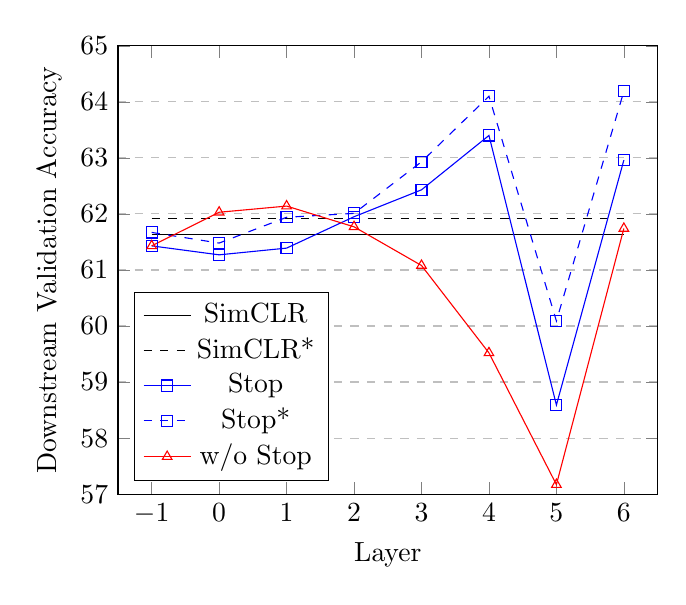
\begin{tikzpicture}
\begin{axis}[
    %title={Temperature dependence of CuSO\(_4\cdot\)5H\(_2\)O solubility},
    % width=0.8\textwidth,
    % height=0.5\textwidth,
    xlabel={Layer},
    ylabel={Downstream Validation Accuracy},
    xmin=-1.5, xmax=6.5,
    ymin=57, ymax=65,
    xtick={-1,0,1,2,3,4,5,6,7}, %,11,12,13},
    ytick={57, 58, 59, 60, 61, 62, 63, 64, 65},
    %ytick={0,0.2,0.4,0.6,0.8,1.0}, %,0.6,0.7,0.8,0.9,1.0},
    legend pos=south west,
    ymajorgrids=true,
    grid style=dashed,
]
\addplot[
    color=black,
    %mark=diamond,
    ]
    coordinates {
    % (300,62.14999771118164)(600,63.15999984741211)(900,62.91999816894531)(1200,62.29999923706055)(1500,61.93000030517578)
    (-1,61.64)
    (0,61.64)
    (1,61.64)
    (2,61.64)
    (3,61.64)
    (4,61.64)
    (5,61.64)
    (6,61.64)
    };
    \addlegendentry{SimCLR}
\addplot[
    %dotted,
    dashed,
    mark options={solid},
    color=black,
    %mark=diamond,
    ]
    coordinates {
    % (300,62.14999771118164)(600,63.15999984741211)(900,62.91999816894531)(1200,62.29999923706055)(1500,61.93000030517578)
    (-1,61.91999816894531)
    (0,61.91999816894531)
    (1,61.91999816894531)
    (2,61.91999816894531)
    (3,61.91999816894531)
    (4,61.91999816894531)
    (5,61.91999816894531)
    (6,61.91999816894531)
    };
    \addlegendentry{SimCLR*}
\addplot[
    color=blue,
    mark=square,
    ]
    coordinates {
    (-1, 61.43000030517578)
    (0, 61.269996643066406) 
    (1, 61.38999938964844)
    (2, 61.94999694824219)
    (3, 62.43000030517578)
    (4, 63.39999771118164)
    (5, 58.59000015258789)
    (6, 62.959999084472656)
    };
    \addlegendentry{Stop}
\addplot[
    dashed,
    mark options={solid},
    color=blue,
    mark=square,
    ]
    coordinates {
    (-1, 61.66999816894531)
    (0, 61.47999954223633)
    (1, 61.939998626708984)
    (2, 62.0099983215332)
    (3, 62.93000030517578)
    (4, 64.0999984741211)
    (5, 60.09000015258789)
    (6, 64.18999481201172)
    };
    \addlegendentry{Stop*}
% \addplot[
%     mark options={solid},
%     color=green,
%     mark=o,
%     ]
%     coordinates {
%     (-1, 61.77)
%     (0, 62.14)
%     (1, 61.84)
%     (2, 61.55)
%     (3, 62.00)
%     (4, 63.83)
%     (5, 63.83)
%     (6, 63.52)
%     };
%     \addlegendentry{debug}
\addplot[
    color=red,
    mark=triangle,
    ]
    coordinates {
    (-1, 61.43000030517578)
    (0, 62.029998779296875)
    (1, 62.13999938964844)
    (2, 61.769996643066406)
    (3, 61.07999801635742)
    (4, 59.519996643066406)
    (5, 57.16999816894531)
    (6, 61.73999786376953)
    };
    \addlegendentry{w/o Stop}
% \addplot[
%     dashed,
%     mark options={solid},
%     color=red,
%     mark=triangle,
%     ]
%     coordinates {
%     (-1, 61.66999816894531)
%     (0, 61.59000015258789)
%     (1, 61.55999755859375)
%     (2, 61.849998474121094)
%     (3, 62.21999740600586)
%     (4, 59.62999725341797)
%     (5, 58.68000030517578)
%     (6, 61.5099983215332)
%     };
%     \addlegendentry{w/o Stop*}


\end{axis}
\end{tikzpicture}
}
%\vspace{-.2in}
%\caption{Continue CIFAR100-CIFAR100}
\caption{Dropout}
\label{fig:CIFAR100-CIFAR100-stop-vs-not-N}
%\vspace{-0.5cm}
\end{subfigure}
\begin{subfigure}{.49\columnwidth}
\resizebox{1.0\columnwidth}{!}{%
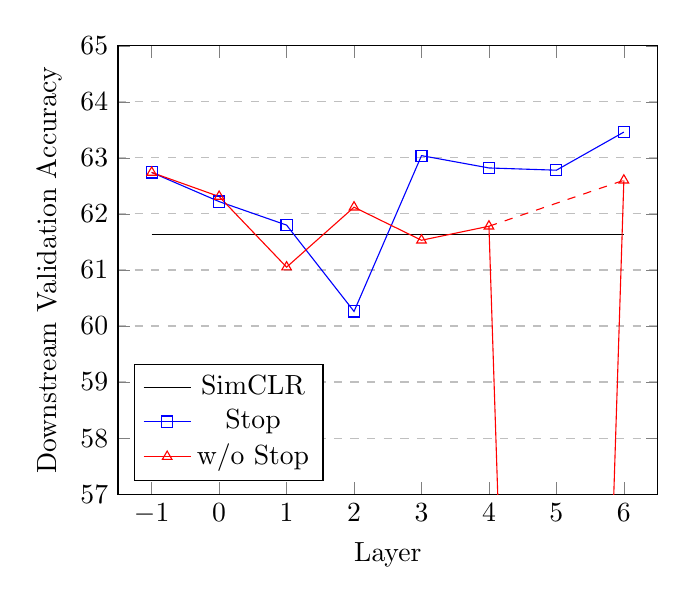
\begin{tikzpicture}
\begin{axis}[
    %title={Temperature dependence of CuSO\(_4\cdot\)5H\(_2\)O solubility},
    % width=0.8\textwidth,
    % height=0.5\textwidth,
    xlabel={Layer},
    ylabel={Downstream Validation Accuracy},
    xmin=-1.5, xmax=6.5,
    ymin=57, ymax=65,
    xtick={-1,0,1,2,3,4,5,6,7}, %,11,12,13},
    ytick={57, 58, 59, 60, 61, 62, 63, 64, 65},
    %ytick={0,0.2,0.4,0.6,0.8,1.0}, %,0.6,0.7,0.8,0.9,1.0},
    legend pos=south west,
    ymajorgrids=true,
    grid style=dashed,
]
\addplot[
    color=black,
    %mark=diamond,
    ]
    coordinates {
    % (300,62.14999771118164)(600,63.15999984741211)(900,62.91999816894531)(1200,62.29999923706055)(1500,61.93000030517578)
    (-1,61.64)
    (6,61.64)
    };
    \addlegendentry{SimCLR}
\addplot[
    %dashed,
    mark options={solid},
    color=blue,
    mark=square,
    ]
    coordinates {
    (-1, 62.74)
    (0, 62.22)
    (1, 61.8)
    (2, 60.26)
    (3, 63.04)
    (4, 62.82)
    (5, 62.78)
    (6, 63.46)
    };
    \addlegendentry{Stop}
\addplot[
    color=red,
    mark=triangle,
    ]
    coordinates {
    (-1, 62.74)
    (0, 62.31)
    (1, 61.05)
    (2, 62.12)
    (3, 61.53)
    (4, 61.78)
    (5, 25.06)
    (6, 62.6)
    };
    \addlegendentry{w/o Stop}
\addplot[
    color=red,
    mark=none,
    dashed,
    ]
    coordinates {
    (4, 61.78)
    (6, 62.6)
    };
\end{axis}
\end{tikzpicture}
}
\caption{PCA}
\label{fig:CIFAR100-CIFAR100-stop-vs-not-pca-6-N}
\end{subfigure}
\vspace{-.05in}
\caption{Contrastive learning. Deep Augmentation with (a) dropout or (b) PCA, with and without stop-gradient. *: initialized with pre-trained SimCLR model. ``Stop'' is short for stop-gradient. Note: Layer 5 is an average pooling.}
% \caption{Comparing sampling 50\% of batch and (a) applying 50\% dropout rate to or (b) subtracting a principal component of that sample, with and without stop-gradient. *: initialized with pre-trained SimCLR model. ``Stop'' is short for stop-gradient. Note: Layer 5 is an average pooling. \vspace{-.2in}}
% \caption{Comparing sampling 50\% of batch and applying 50\% dropout rate to that sample, with and without stop-gradient. *: initialized with pre-trained SimCLR model. ``Stop'' is short for stop-gradient.\vspace{-.2in}}
\end{figure}


% \subsubsection{Initialization \& Freezing Weights}
% \label{sec:Initialization-and-Freezing-Weights}

\textbf{Initialization \& Freezing Weights.}
Augmentations may have a more significant impact on higher layers that already possess useful, discriminative features. In addition, the concurrent objectives of learning features and maintaining invariance to their alterations could conflict, slowing down or destabilizing training. In Figure \ref{fig:CIFAR100-CIFAR100-stop-vs-not-N}, `SimCLR*' and `Stop*' show results using SimCLR and Deep Augmentation with stop-gradient (resp.), starting with weights from a SimCLR pre-trained network on CIFAR100. Despite Deep Augmentation showing a marginal superiority over SimCLR in terms of initialization, the advantages of pre-training before applying Deep Augmentation are minimal. This indicates that pre-training a neural network is not crucial for Deep Augmentation. 
%
Further, freezing layers before or after the targeted layer, with pre-trained SimCLR weights on CIFAR, did not yield competitive performance; see Appendix \ref{appendix:freezing-layers}.

% A larger impact of augmentations may be observed in higher network layers if the network has already developed useful and discriminative features up to those levels. In addition, the concurrent objectives of learning features and maintaining invariance to their alterations could conflict, potentially slowing down the training process or leading to instability. As illustrated in Figure \ref{fig:CIFAR100-CIFAR100-stop-vs-not-N}, `SimCLR*' and `Stop*' represent scenarios where training is conducted using SimCLR or layer-targeted dropout with stop-gradient, but with the initial weights from a neural network pre-trained on CIFAR100 using SimCLR. While Deep Augmentation shows a marginal superiority over SimCLR in terms of benefitting from this initialization, the differences are not substantial. This indicates that pre-training a neural network is not a crucial prerequisite for the successful use of Deep Augmentation.

% In a related exploration, we investigated the effect of freezing either the layers up to and including, or those following, the targeted layer in Deep Augmentation, using the pre-trained weights of a neural network trained on CIFAR using SimCLR. This approach did not yield competitive performance levels. Detailed results and further discussion on this aspect are presented in the Appendix.

%\subsubsection{PCA-Augmentation}

% In this section, we evaluate whether dropout is the sole effective augmentation technique within the Deep Augmentation framework. In contrast to the traditional method of dropping individual neurons as done in dropout, we experimented with the subtraction of a principal component in the feature space. More formally, for a mini-batch with indices denoted as $I_b = {1,2,\dots,K}$, the augmentation for a sample $x_i, i \in I_b$ is defined as follows:
% \begin{align*}
% A_p(x_i, z_i^j) = x_i - PC(\{ x_k : k \in I_b \})[:,p]
% \end{align*}
% where $PC$ calculates the principal components of the set and arranges them in descending order of their eigenvalues. The batch is centered prior to this operation and re-centered afterwards. We tested this method, hereafter referred to as

% \textbf{PCA-Augmentation.}
% We evaluate the PCA-augmentation, with $p=1$ and $p=6$, corresponding to the removal of the largest and the sixth largest principal components, respectively. The results indicated that $p=6$ yielded superior performance compared to $p=1$. Figure \ref{fig:CIFAR100-CIFAR100-stop-vs-not-pca-6-N} presents the results for $p=6$ both with and without the application of stop-gradient. For the results corresponding to $p=1$, refer to the Appendix.

% Similar to the observations with dropout, the application of stop-gradient consistently resulted in enhanced performance, especially when targeted at higher layers.

% \begin{figure}[ht]
% \centering
% \begin{subfigure}{.49\columnwidth}
% \resizebox{1.0\columnwidth}{!}{%
% \begin{tikzpicture}
% \begin{axis}[
%     %title={Temperature dependence of CuSO\(_4\cdot\)5H\(_2\)O solubility},
%     % width=0.8\textwidth,
%     % height=0.5\textwidth,
%     xlabel={Layer},
%     ylabel={Downstream Validation Accuracy},
%     xmin=-1.5, xmax=6.5,
%     ymin=57, ymax=65,
%     xtick={-1,0,1,2,3,4,5,6,7}, %,11,12,13},
%     ytick={57, 58, 59, 60, 61, 62, 63, 64, 65},
%     %ytick={0,0.2,0.4,0.6,0.8,1.0}, %,0.6,0.7,0.8,0.9,1.0},
%     legend pos=south west,
%     ymajorgrids=true,
%     grid style=dashed,
% ]
% \addplot[
%     color=black,
%     %mark=diamond,
%     ]
%     coordinates {
%     % (300,62.14999771118164)(600,63.15999984741211)(900,62.91999816894531)(1200,62.29999923706055)(1500,61.93000030517578)
%     (-1,61.64)
%     (6,61.64)
%     };
%     \addlegendentry{SimCLR}
% \addplot[
%     %dashed,
%     mark options={solid},
%     color=blue,
%     mark=square,
%     ]
%     coordinates {
%     (-1, 62.74)
%     (0, 62.22)
%     (1, 61.8)
%     (2, 60.26)
%     (3, 63.04)
%     (4, 62.82)
%     (5, 62.78)
%     (6, 63.46)
%     };
%     \addlegendentry{Stop}
% \addplot[
%     color=red,
%     mark=triangle,
%     ]
%     coordinates {
%     (-1, 62.74)
%     (0, 62.31)
%     (1, 61.05)
%     (2, 62.12)
%     (3, 61.53)
%     (4, 61.78)
%     (5, 25.06)
%     (6, 62.6)
%     };
%     \addlegendentry{w/o Stop}
% \addplot[
%     color=red,
%     mark=none,
%     dashed,
%     ]
%     coordinates {
%     (4, 61.78)
%     (6, 62.6)
%     };
% \end{axis}
% \end{tikzpicture}
% }
% \end{subfigure}
% \vspace{-.2in}
% %\caption{Continue CIFAR100-CIFAR100}
% \caption{PCA: Comparing sampling 50\% of batch and subtracting the 6-th larget principal component from that sample, with and without stop-gradient. ``Stop'' is short for stop-gradient. Note that Layer 5 is an average pooling.\vspace{-.2in}}
% \label{fig:CIFAR100-CIFAR100-stop-vs-not-pca-6-N}
% %\vspace{-0.5cm}
% \end{figure}

%\subsubsection{Supervised Learning}

\textbf{Supervised Learning.}
We investigate Deep Augmentation in the context of supervised learning, comparing its efficacy to that in contrastive learning (Figures \ref{fig:CIFAR100-CIFAR100-stop-vs-not-supervised-N} and \ref{fig:CIFAR100-CIFAR100-stop-vs-not-supervised-pca6}). Deep Augmentation, whether through dropout or PCA, does not enhance performance in supervised learning on the CIFAR dataset. Notably, the absence of stop-gradient  yielded superior results compared to its inclusion, diverging from the trend in contrastive learning. While Deep Augmentation appears to detract from performance in supervised learning, retaining data augmentations is crucial, as their omission resulted in a significant drop in accuracy to 59.02\%.

\begin{figure}
\centering
\begin{subfigure}{.33\columnwidth}
\centering
\resizebox{1.0\columnwidth}{!}{%
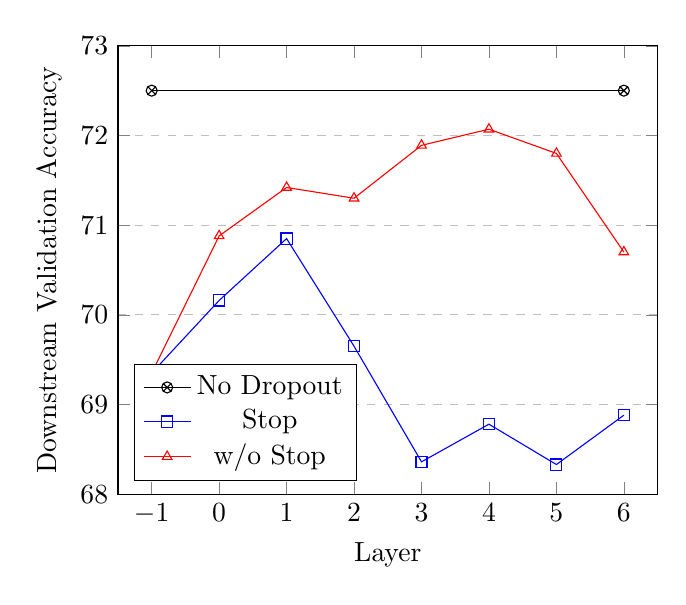
\begin{tikzpicture}
\begin{axis}[
    xlabel={Layer},
    ylabel={Downstream Validation Accuracy},
    xmin=-1.5, xmax=6.5,
    ymin=68, ymax=73,
    xtick={-1,0,1,2,3,4,5,6,7}, %,11,12,13},
    ytick={68, 69, 70, 71, 72, 73}, %57, 58, 59, 60, 61, 62, 63, 64, 65},
    legend pos=south west,
    ymajorgrids=true,
    grid style=dashed,
]
\addplot+[color=black, mark=otimes, error bars/.cd, y dir=both, y explicit, 
    ] coordinates {
    (-1, 72.5) %+- (0, 0.248797)
    (6, 72.5) %+- (0, 0.248797)
    };
    \addlegendentry{No Dropout}
\addplot+[color=blue, mark=square, error bars/.cd, y dir=both, y explicit, 
    ] coordinates {
    (-1, 69.35) %+- (0,0.19)
    (0, 70.16) %+- (0,0.10)
    (1, 70.85) %+- (0,0.21)
    (2, 69.65) %+- (0,0.27)
    (3, 68.36) %+- (0,0.20)
    (4, 68.78) %+- (0,0.18)
    (5, 68.33) %+- (0,0.26)
    (6, 68.88) %+- (0,0.09)
    };
    \addlegendentry{Stop}
% \addplot+[color=green, mark=square, error bars/.cd, y dir=both, y explicit, 
%     ] coordinates {
%     (-1, 71.82)
%     (0, 71.45)
%     (1, 71.1) 
%     (2, 69.83) 
%     (3, 68.5) 
%     (4, 68.94)
%     (5, 68.94)
%     (6, 69.02) 
%     };
%     \addlegendentry{debug}
\addplot+[color=red, mark=triangle, error bars/.cd, y dir=both, y explicit, 
    ] 
    coordinates {
    (-1, 69.35) %+- (0,0.19)
    (0, 70.88) %+- (0,0.19)
    (1, 71.42) %+- (0,0.25)
    (2, 71.30) %+- (0,0.28)
    (3, 71.89) %+- (0,0.03)
    (4, 72.07) %+- (0,0.18)
    (5, 71.80) %+- (0,0.25)
    (6, 70.70) %+- (0,0.24)
    };
    \addlegendentry{w/o Stop}
\end{axis}
\end{tikzpicture}
}
%\vspace{-.2in}
%\caption{Continue CIFAR100-CIFAR100}
\caption{Dropout}
\label{fig:CIFAR100-CIFAR100-stop-vs-not-supervised-N}
\end{subfigure}%
%\hspace{0.2in}
\hspace{0.2in}
\begin{subfigure}{.33\columnwidth}
\centering
\resizebox{1.0\columnwidth}{!}{%
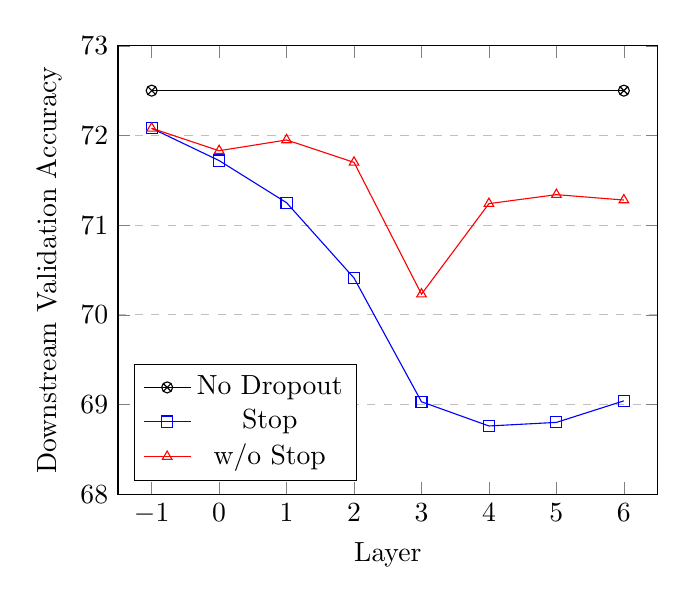
\begin{tikzpicture}
\begin{axis}[
    xlabel={Layer},
    ylabel={Downstream Validation Accuracy},
    xmin=-1.5, xmax=6.5,
    ymin=68, ymax=73,
    xtick={-1,0,1,2,3,4,5,6,7}, %,11,12,13},
    ytick={68, 69, 70, 71, 72, 73}, %57, 58, 59, 60, 61, 62, 63, 64, 65},
    legend pos=south west,
    ymajorgrids=true,
    grid style=dashed,
]
\addplot+[color=black, mark=otimes, error bars/.cd, y dir=both, y explicit, 
    ] coordinates {
    (-1, 72.5) %+- (0, 0.248797)
    (6, 72.5) %+- (0, 0.248797)
    };
    \addlegendentry{No Dropout}
% \addplot+[color=blue, mark=square, error bars/.cd, y dir=both, y explicit, 
%     ] coordinates {
%     (-1, 71.84) +- (0,0.09)
%     (0, 71.52) +- (0,0.15)
%     (1, 71.03) +- (0,0.13)
%     (2, 70.11) +- (0,0.11)
%     (3, 69.00) +- (0,0.17)
%     (4, 69.54) +- (0,0.51)
%     (5, 69.49) +- (0,0.15)
%     (6, 69.04) +- (0,0.28)
%     };
%     \addlegendentry{1 Stop}
% \addplot+[color=red, mark=triangle, error bars/.cd, y dir=both, y explicit, 
%     ] 
%     coordinates {
%     (-1, 71.84) +- (0,0.09)
%     (0, 71.93) +- (0,0.39)
%     (1, 71.91) +- (0,0.08)
%     (2, 71.73) +- (0,0.07)
%     (3, 71.94) +- (0,0.20)
%     (4, 71.63) +- (0,0.34)
%     (5, 71.52) +- (0,0.09)
%     (6, 71.70) +- (0,0.13)
%     };
%     \addlegendentry{1 w/o Stop}
\addplot+[color=blue, mark=square, error bars/.cd, y dir=both, y explicit, 
    ] coordinates {
    (-1, 72.08) %+- (0,0.40)
    (0, 71.72) %+- (0,0.24)
    (1, 71.25) %+- (0,0.12)
    (2, 70.41) %+- (0,0.08)
    (3, 69.03) %+- (0,0.28)
    (4, 68.76) %+- (0,0.20)
    (5, 68.80) % +- (0,0.14)
    (6, 69.04) % +- (0,0.28)
    };
    \addlegendentry{Stop}
\addplot+[color=red, mark=triangle, error bars/.cd, y dir=both, y explicit, 
    ] 
    coordinates {
    (-1, 72.08) %+- (0,0.40)
    (0, 71.83) %+- (0,0.31)
    (1, 71.95) %+- (0,0.05)
    (2, 71.70) %+- (0,0.15)
    (3, 70.23) %+- (0,2.02)
    (4, 71.24) %+- (0,0.33)
    (5, 71.34) %+- (0,0.02)
    (6, 71.28) %+- (0,0.33)
    };
    \addlegendentry{w/o Stop}
\end{axis}
\end{tikzpicture}
}
\vspace{-.2in}
%\caption{Continue CIFAR100-CIFAR100}
\caption{PCA}
\label{fig:CIFAR100-CIFAR100-stop-vs-not-supervised-pca6}
%\vspace{-0.5cm}
\end{subfigure}
\vspace{-.1in}
\caption{Supervised only. Deep Augmentation with (a) dropout or (b) PCA, with and without stop-gradient. *: initialized with pre-trained SimCLR model. ``Stop'' is short for stop-gradient. \vspace{-.1in}}
%\caption{Supervised only. Comparing sampling 50\% of batch and (a) applying 50\% dropout rate to or (b) removing the 6-th largest principal component from that sample, with and without stop-gradient. ``Stop'' is short for stop-gradient. No data augmentations: 59.02\%.}
%\vspace{-.1in}
\label{fig:CIFAR100-supervised}
\end{figure}

\subsection{Graphs}

Next, we explore transferability of Deep Augmentation insights from vision and sentence embeddings to graph contrastive learning, assessing applicability across modalities.

% This section explore if the insights from Vision and Sentence embeddings apply to graph contrastive learning.

%Now we explore if the insights from Vision and Sentence Embeddings apply to graphs.

%\subsubsection{Augmentation, Layer, and Stop-Gradient}

\textbf{Augmentation, Layer, and Stop-Gradient.}
We apply Deep Augmentation to graph datasets including COLLAB, IMDB-Multi, NCI1, and PROTEINS, integrating it with standard graph data augmentation techniques. The results of Deep Augmentation using dropout and PCA (targeting the 6th largest principal component) are presented in Figures \ref{fig:graphs-dropout-N} and \ref{fig:graphs-PCA-N}, respectively. Notably, due to the variable embedding size of each graph neural network (GNN) sample within a batch, we adapted the PCA to operate over all node embeddings.

While trends across these datasets are not uniform, Deep Augmentation, particularly when with dropout and stop-gradient, significantly enhanced performance on all  datasets. % except IMDB-Multi.


\begin{figure}[ht]
\begin{subfigure}{.245\columnwidth}
\centering
\resizebox{1.0\columnwidth}{!}{%
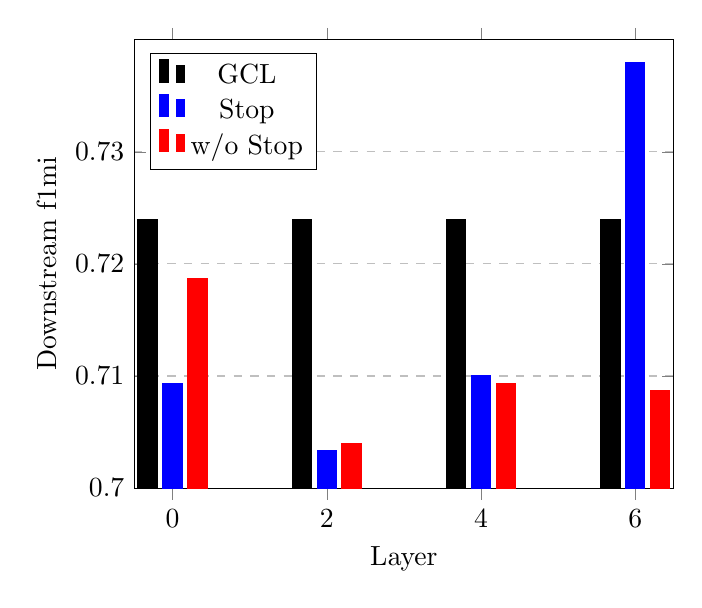
\begin{tikzpicture}
\begin{axis}[
    xlabel={Layer},
    ylabel={Downstream f1mi},
    xmin=-0.5, xmax=6.5,
    ymin=0.70, ymax=0.74,
    xtick={-1,0,2,4,6,7},
    ytick={0.68,0.69,0.70,0.71,0.72,0.73},
    legend pos=north west,
    ymajorgrids=true,
    grid style=dashed,
    ybar, % Enable bar plots
    bar width=7pt, % Adjust the bar width as needed
    % Other bar plot configurations can be added here
]
\addplot+[color=black, mark=none, %y dir=both, y explicit, error bars/.cd
    ] coordinates {
    (0, 0.7239999969800314)
    (2, 0.7239999969800314)
    (4, 0.7239999969800314)
    (6, 0.7239999969800314)
    };
     \addlegendentry{GCL}
    
\addplot+[color=blue, % y dir=both, y explicit, % error bars/.cd, mark=square
    ] coordinates {
(0, 0.709333340326945)
(2, 0.703333338101705)
(4, 0.7099999984105428)
(6, 0.7379999955495199)
    };
    \addlegendentry{Stop}
    
\addplot+[color=red, % y dir=both, y explicit, % error bars/.cd,  mark=triangle
    ] 
    coordinates {
    (0, 0.718666652838389)
    (2, 0.7039999961853027)
    (4, 0.7093333204587301) 
    (6, 0.7086666822433472)
    };
    \addlegendentry{w/o Stop}
\end{axis}
\end{tikzpicture}
% \begin{tikzpicture}
% \begin{axis}[
%     %title={Temperature dependence of CuSO\(_4\cdot\)5H\(_2\)O solubility},
%     % width=0.8\textwidth,
%     % height=0.5\textwidth,
%     xlabel={Layer},
%     ylabel={Downstream f1mi},
%     xmin=-0.5, xmax=6.5,
%     ymin=0.70, ymax=0.74,
%     xtick={-1,0,1,2,3,4,5,6,7}, %,11,12,13},
%     ytick={0.68,0.69,0.70,0.71,0.72,0.73}, %57, 58, 59, 60, 61, 62, 63, 64, 65},
%     %ytick={0,0.2,0.4,0.6,0.8,1.0}, %,0.6,0.7,0.8,0.9,1.0},
%     legend pos=north west,
%     ymajorgrids=true,
%     grid style=dashed,
% ]
% \addplot+[color=black, mark=none, error bars/.cd, y dir=both, y explicit, 
%     ] coordinates {
%     (0, 0.7239999969800314) %+- (0,0.007451075926921274)
%     (6, 0.7239999969800314) %+- (0,0.007451075926921274) 0.7239999969800314 0.7379999955495199
%     };
%      \addlegendentry{Dropout}
    
% \addplot+[color=blue, mark=square, error bars/.cd, y dir=both, y explicit, 
%     ] coordinates {
% (0, 0.709333340326945)
% (2, 0.703333338101705)
% (4, 0.7099999984105428)
% (6, 0.7379999955495199)
%     };
%     \addlegendentry{Stop}
    
% \addplot+[color=red, mark=triangle, error bars/.cd, y dir=both, y explicit, 
%     ] 
%     coordinates {
%     (0, 0.718666652838389)
%     (2, 0.7039999961853027)
%     (4, 0.7093333204587301) 
%     (6, 0.7086666822433472)
%     };
%     \addlegendentry{w/o Stop}
% \end{axis}
% \end{tikzpicture}
}
%\vspace{-.2in}
%\caption{Continue CIFAR100-CIFAR100}
%\vspace{-.09in}
\caption{COLLAB}
\label{fig:graphs-collab-r}
%\vspace{-0.5cm}
\end{subfigure}
\begin{subfigure}{.245\columnwidth}
\centering
\resizebox{1.0\columnwidth}{!}{%
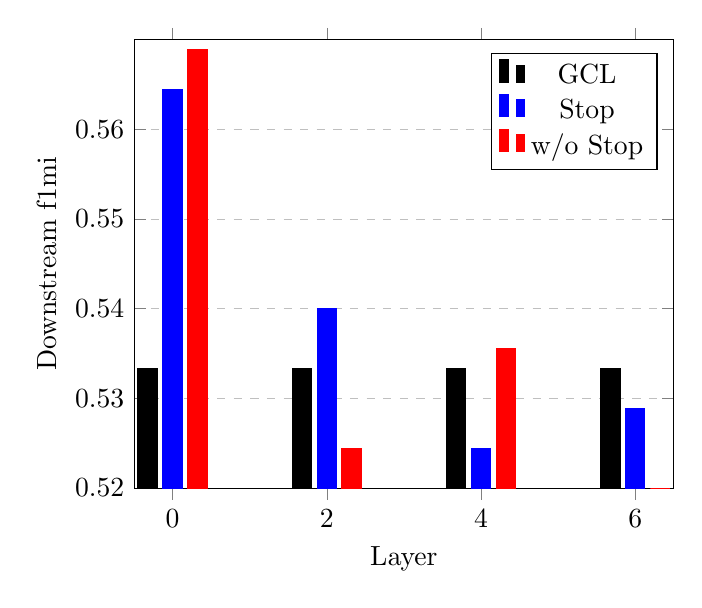
\begin{tikzpicture}
\begin{axis}[
    xlabel={Layer},
    ylabel={Downstream f1mi},
    xmin=-0.5, xmax=6.5,
    ymin=0.52, ymax=0.57,
    xtick={-1,0,2,4,6,7}, %,11,12,13},
    ytick={0.44,0.45,0.46,0.47,0.48,0.49,0.50,0.51,0.52,0.53,0.54,0.55,0.56,0.68,0.69,0.70,0.71,0.72,0.73}, %57, 58, 59, 60, 61, 62, 63, 64, 65},
    legend pos=north east,
    ymajorgrids=true,
    grid style=dashed,
    ybar, % Enable bar plots
    bar width=7pt, % Adjust the bar width as needed
    % Other bar plot configurations can be added here
]
\addplot+[color=black, mark=none, %y dir=both, y explicit, error bars/.cd
    ] coordinates {
    (0, 0.5333333412806193)
    (2, 0.5333333412806193)
    (4, 0.5333333412806193)
    (6, 0.5333333412806193) % 
    };
     \addlegendentry{GCL}
    
\addplot+[color=blue, % y dir=both, y explicit, % error bars/.cd, mark=square
    ] coordinates {
    (0, 0.5644444425900778)  
    (2, 0.5400000015894572)
    (4, 0.5244444310665131)
    (6, 0.5288888812065125) 
    };
    \addlegendentry{Stop}
    
\addplot+[color=red, % y dir=both, y explicit, % error bars/.cd,  mark=triangle
    ] 
    coordinates {
    (0, 0.5688889026641846)
    (2, 0.5244444410006205)
    (4, 0.5355555613835653)
    (6, 0.5200000007947286)
    };
    \addlegendentry{w/o Stop}
\end{axis}
\end{tikzpicture}
% \begin{tikzpicture}
% \begin{axis}[
%     %title={Temperature dependence of CuSO\(_4\cdot\)5H\(_2\)O solubility},
%     % width=0.8\textwidth,
%     % height=0.5\textwidth,
%     xlabel={Layer},
%     ylabel={Downstream f1mi},
%     xmin=-0.5, xmax=6.5,
%     ymin=0.52, ymax=0.57,
%     xtick={-1,0,1,2,3,4,5,6,7}, %,11,12,13},
%     ytick={0.44,0.45,0.46,0.47,0.48,0.49,0.50,0.51,0.52,0.53,0.54,0.55,0.56,0.68,0.69,0.70,0.71,0.72,0.73}, %57, 58, 59, 60, 61, 62, 63, 64, 65},
%     %ytick={0,0.2,0.4,0.6,0.8,1.0}, %,0.6,0.7,0.8,0.9,1.0},
%     legend pos=north east,
%     ymajorgrids=true,
%     grid style=dashed,
% ]
% \addplot+[color=black, mark=none, error bars/.cd, y dir=both, y explicit, 
%     ] coordinates {
%     (0, 0.5333333412806193)
%     (6, 0.5333333412806193) % 
%     };
%     \addlegendentry{Dropout}    
% \addplot+[color=blue, mark=square, error bars/.cd, y dir=both, y explicit, 
%     ] coordinates {
%     (0, 0.5644444425900778)  
%     (2, 0.5400000015894572)
%     (4, 0.5244444310665131)
%     (6, 0.5288888812065125)
%     };
%     \addlegendentry{Stop}
    
% \addplot+[color=red, mark=triangle, error bars/.cd, y dir=both, y explicit, 
%     ] 
%     coordinates {
%     (0, 0.5688889026641846)
%     (2, 0.5244444410006205)
%     (4, 0.5355555613835653)
%     (6, 0.5200000007947286)
%     };
%     \addlegendentry{w/o Stop}
% \end{axis}
% \end{tikzpicture}
}
%\vspace{-.2in}
%\caption{Continue CIFAR100-CIFAR100}
\caption{IMDB-Multi}
\label{fig:graphs-imdb-multi-r}
%\vspace{-0.5cm}
\end{subfigure}
\begin{subfigure}{.245\columnwidth}
\centering
\resizebox{1.0\columnwidth}{!}{%
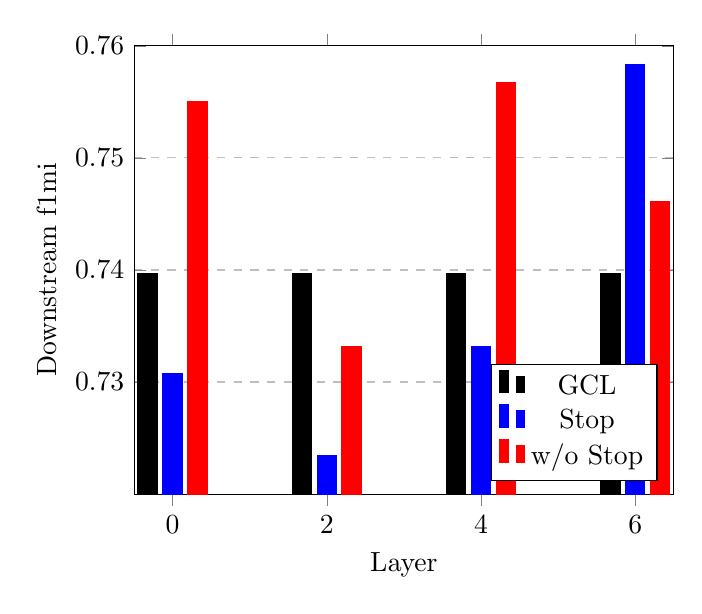
\begin{tikzpicture}
\begin{axis}[
    %title={Temperature dependence of CuSO\(_4\cdot\)5H\(_2\)O solubility},
    % width=0.8\textwidth,
    % height=0.5\textwidth,
    xlabel={Layer},
    ylabel={Downstream f1mi},
    xmin=-0.5, xmax=6.5,
    ymin=0.72, ymax=0.76,
    xtick={-1,0,2,4,6,7}, %,11,12,13},
    ytick={0.73, 0.74, 0.75, 0.76,0.77,0.78,0.79,0.80,0.81,0.82,0.83,0.84,0.85}, %57, 58, 59, 60, 61, 62, 63, 64, 65},
    %ytick={0,0.2,0.4,0.6,0.8,1.0}, %,0.6,0.7,0.8,0.9,1.0},
    legend pos=south east,
    ymajorgrids=true,
    grid style=dashed,
    ybar, % Enable bar plots
    bar width=7pt, % Adjust the bar width as needed
]
\addplot+[color=black,% mark=none, error bars/.cd, y dir=both, y explicit, 
    ] coordinates {
    (0, 0.7396593689918518)
    (2, 0.7396593689918518)
    (4, 0.7396593689918518)
    (6, 0.7396593689918518) % 0.739659 0.758313
    };
    \addlegendentry{GCL}
    
\addplot+[color=blue, %mark=square, error bars/.cd, y dir=both, y explicit, 
    ] coordinates {
    (0, 0.7307380437850952)
    (2, 0.7234387795130411)
    (4, 0.7331711252530416)
    (6, 0.7583130399386088)
    };
    \addlegendentry{Stop}
    
\addplot+[color=red, %mark=triangle, error bars/.cd, y dir=both, y explicit, 
    ] 
    coordinates {
    (0, 0.7550689379374186)
    (2, 0.7331711451212565)
    (4, 0.7566909790039062)
    (6, 0.7461475928624471)
    };
    \addlegendentry{w/o Stop}
\end{axis}
\end{tikzpicture}
}
%\vspace{-.2in}
%\caption{Continue CIFAR100-CIFAR100}
\caption{NCI1}
\label{fig:graphs-nci1-r}
%\vspace{-0.5cm}
\end{subfigure}
\begin{subfigure}{.245\columnwidth}
\centering
\resizebox{1.0\columnwidth}{!}{%
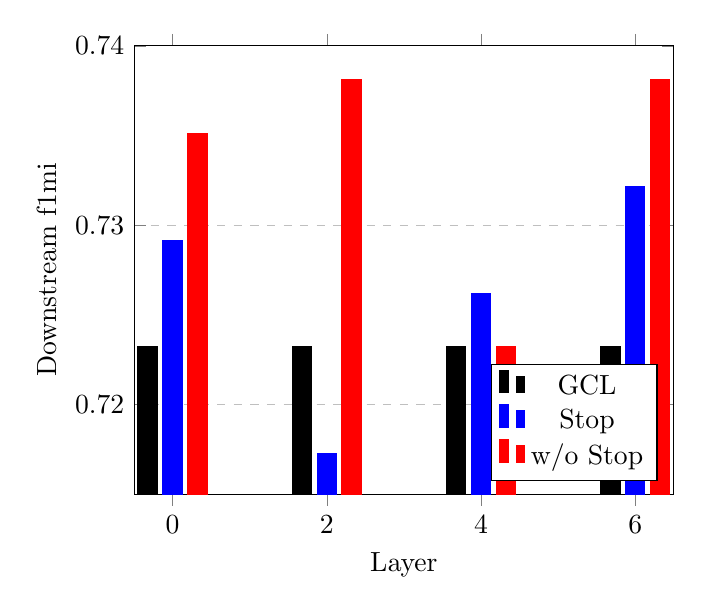
\begin{tikzpicture}
\begin{axis}[
    %title={Temperature dependence of CuSO\(_4\cdot\)5H\(_2\)O solubility},
    % width=0.8\textwidth,
    % height=0.5\textwidth,
    xlabel={Layer},
    ylabel={Downstream f1mi},
    xmin=-0.5, xmax=6.5,
    ymin=0.715, ymax=0.74,
    xtick={-1,0,2,4,6,7}, %,11,12,13},
    ytick={0.69,0.70,0.71,0.72,0.73,0.74,0.75,0.76,0.77,0.78,0.79,0.80,0.81,0.82,0.83}, %57, 58, 59, 60, 61, 62, 63, 64, 65},
    %ytick={0,0.2,0.4,0.6,0.8,1.0}, %,0.6,0.7,0.8,0.9,1.0},
    legend pos=south east,
    ymajorgrids=true,
    grid style=dashed,
    ybar, % Enable bar plots
    bar width=7pt, % Adjust the bar width as needed
]
\addplot+[color=black, % mark=none, error bars/.cd, y dir=both, y explicit, 
    ] coordinates {
    (0, 0.7232142686843872) % +- 0.014580289135568155
    (2, 0.7232142686843872)
    (4, 0.7232142686843872)
    (6,0.7232142686843872) % 72.32 73.81
    };
    \addlegendentry{GCL}

    
\addplot+[color=blue,% mark=square, error bars/.cd, y dir=both, y explicit, 
    ] coordinates {
    (0, 0.7291666666666666)
    (2, 0.7172619104385376)
    (4, 0.726190467675527)
    (6, 0.7321428656578064) 
    };
    \addlegendentry{Stop}
    
\addplot+[color=red, %mark=triangle, error bars/.cd, y dir=both, y explicit, 
    ] 
    coordinates {
    (0, 0.7351190447807312)
    (2, 0.738095223903656)
    (4, 0.7232142885526022)
    (6, 0.738095243771871)
    };
    \addlegendentry{w/o Stop}
\end{axis}
\end{tikzpicture}
}
%\vspace{-.2in}
%\caption{Continue CIFAR100-CIFAR100}
\caption{PROTEINS}
\label{fig:graphs-proteins-r}
%\vspace{-0.5cm}
\end{subfigure}
\vspace{-.1in}
\caption{Graphs: Deep Augmentation with Dropout}
\label{fig:graphs-dropout-N}%\vspace{-.1in}
\end{figure}



\begin{figure}[ht]
\begin{subfigure}{.245\columnwidth}
\centering
\resizebox{1.0\columnwidth}{!}{%
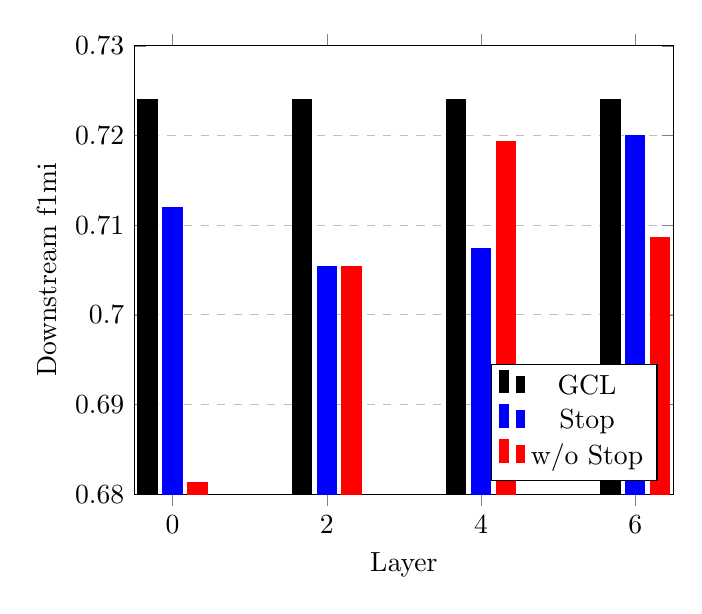
\begin{tikzpicture}
\begin{axis}[
    %title={Temperature dependence of CuSO\(_4\cdot\)5H\(_2\)O solubility},
    % width=0.8\textwidth,
    % height=0.5\textwidth,
    xlabel={Layer},
    ylabel={Downstream f1mi},
    xmin=-0.5, xmax=6.5,
    ymin=0.68, ymax=0.73,
    xtick={-1,0,2,4,6,7}, %,11,12,13},
    ytick={0.68,0.69,0.70,0.71,0.72,0.73}, %57, 58, 59, 60, 61, 62, 63, 64, 65},
    %ytick={0,0.2,0.4,0.6,0.8,1.0}, %,0.6,0.7,0.8,0.9,1.0},
    legend pos=south east,
    ymajorgrids=true,
    grid style=dashed,
    ybar, % Enable bar plots
    bar width=7pt, % Adjust the bar width as needed
]
\addplot+[color=black, % mark=none, error bars/.cd, y dir=both, y explicit, 
    ] coordinates {
    (0, 0.7239999969800314) %+- (0,0.007451075926921274)
    (2, 0.7239999969800314)
    (4, 0.7239999969800314)
    (6, 0.7239999969800314) %+- (0,0.007451075926921274)
    };
     \addlegendentry{GCL}
    
\addplot+[color=blue, % mark=square, error bars/.cd, y dir=both, y explicit, 
    ] coordinates {
    (0, 0.7119999925295512)
    (2, 0.7053333123524984)
    (4, 0.7073333462079366)
    (6, 0.7200000087420145)
    };
    \addlegendentry{Stop}
    
\addplot+[color=red, % mark=triangle, error bars/.cd, y dir=both, y explicit, 
    ] 
    coordinates {
    (0, 0.681333323319753)
    (2, 0.7053333322207133)
    (4, 0.7193333307902018) 
    (6, 0.7086666425069174)
    };
    \addlegendentry{w/o Stop}
\end{axis}
\end{tikzpicture}
}
\vspace{-.2in}
%\caption{Continue CIFAR100-CIFAR100}
\caption{COLLAB}
\label{fig:graphs-collab-r}
%\vspace{-0.5cm}
\end{subfigure}
\begin{subfigure}{.245\columnwidth}
\centering
\resizebox{1.0\columnwidth}{!}{%
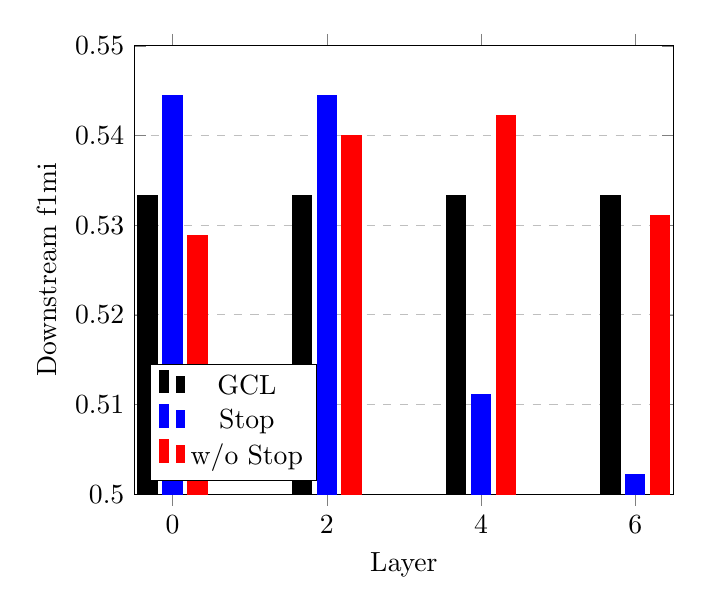
\begin{tikzpicture}
\begin{axis}[
    %title={Temperature dependence of CuSO\(_4\cdot\)5H\(_2\)O solubility},
    % width=0.8\textwidth,
    % height=0.5\textwidth,
    xlabel={Layer},
    ylabel={Downstream f1mi},
    xmin=-0.5, xmax=6.5,
    ymin=0.50, ymax=0.55,
    xtick={-1,0,2,4,6,7}, %,11,12,13},
    ytick={0.44,0.45,0.46,0.47,0.48,0.49,0.50,0.51,0.52,0.53,0.54,0.55,0.56,0.68,0.69,0.70,0.71,0.72,0.73}, %57, 58, 59, 60, 61, 62, 63, 64, 65},
    %ytick={0,0.2,0.4,0.6,0.8,1.0}, %,0.6,0.7,0.8,0.9,1.0},
    legend pos=south west,
    ymajorgrids=true,
    grid style=dashed,
    ybar, % Enable bar plots
    bar width=7pt, 
]
\addplot+[color=black, %mark=none, error bars/.cd, y dir=both, y explicit, 
    ] coordinates {
    (0, 0.5333333412806193)
    (2, 0.5333333412806193)
    (4, 0.5333333412806193)
    (6, 0.5333333412806193)
    };
    \addlegendentry{GCL}    
\addplot+[color=blue, %mark=square, error bars/.cd, y dir=both, y explicit, 
    ] coordinates {
    (0, 0.5444444616635641)
    (2, 0.5444444417953491)
    (4, 0.5111111203829447)
    (6, 0.5022222101688385)
    };
    \addlegendentry{Stop}
    
\addplot+[color=red, %mark=triangle, error bars/.cd, y dir=both, y explicit, 
    ] 
    coordinates {
    (0, 0.5288888911406199)
    (2, 0.5400000015894572)
    (4, 0.542222241560618)
    (6, 0.5311111211776733)
    };
    \addlegendentry{w/o Stop}
\end{axis}
\end{tikzpicture}
}
\vspace{-.2in}
%\caption{Continue CIFAR100-CIFAR100}
\caption{IMDB-Multi}
\label{fig:graphs-imdb-multi-r}
%\vspace{-0.5cm}
\end{subfigure}
\begin{subfigure}{.245\columnwidth}
\centering
\resizebox{1.0\columnwidth}{!}{%
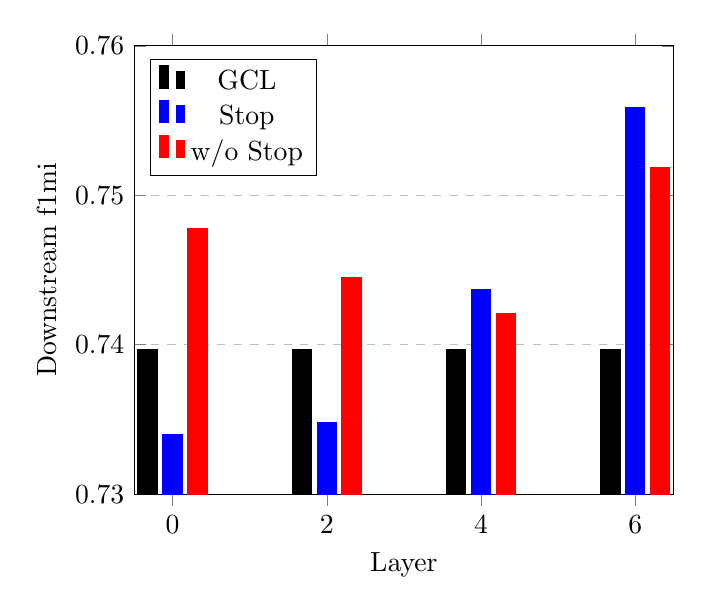
\begin{tikzpicture}
\begin{axis}[
    %title={Temperature dependence of CuSO\(_4\cdot\)5H\(_2\)O solubility},
    % width=0.8\textwidth,
    % height=0.5\textwidth,
    xlabel={Layer},
    ylabel={Downstream f1mi},
    xmin=-0.5, xmax=6.5,
    ymin=0.73, ymax=0.76,
    xtick={-1,0,2,4,6,7}, %,11,12,13},
    ytick={0.73, 0.74, 0.75, 0.76,0.77,0.78,0.79,0.80,0.81,0.82,0.83,0.84,0.85}, %57, 58, 59, 60, 61, 62, 63, 64, 65},
    %ytick={0,0.2,0.4,0.6,0.8,1.0}, %,0.6,0.7,0.8,0.9,1.0},
    legend pos=north west,
    ymajorgrids=true,
    grid style=dashed,
    ybar, % Enable bar plots
    bar width=7pt, % Adjust the bar width as needed
]
\addplot+[color=black, %mark=none, error bars/.cd, y dir=both, y explicit, 
    ] coordinates {
    (0, 0.7396593689918518)
    (2, 0.7396593689918518)
    (4, 0.7396593689918518)
    (6, 0.7396593689918518)
    };
    \addlegendentry{GCL}
    
\addplot+[color=blue, %mark=square, error bars/.cd, y dir=both, y explicit, 
    ] coordinates {
    (0, 0.7339821656545004)
    (2, 0.7347931861877441)
    (4, 0.7437145113945007)
    (6,0.7558799584706625)
    };
    \addlegendentry{Stop}
    
\addplot+[color=red, %mark=triangle, error bars/.cd, y dir=both, y explicit, 
    ] 
    coordinates {
    (0, 0.7477696537971497)
    (2, 0.7445255319277445)
    (4, 0.7420924504597982)
    (6, 0.7518248160680135)
    };
    \addlegendentry{w/o Stop}
\end{axis}
\end{tikzpicture}
}
\vspace{-.2in}
%\caption{Continue CIFAR100-CIFAR100}
\caption{NCI1}
\label{fig:graphs-nci1-r}
%\vspace{-0.5cm}
\end{subfigure}
\begin{subfigure}{.245\columnwidth}
\centering
\resizebox{1.0\columnwidth}{!}{%
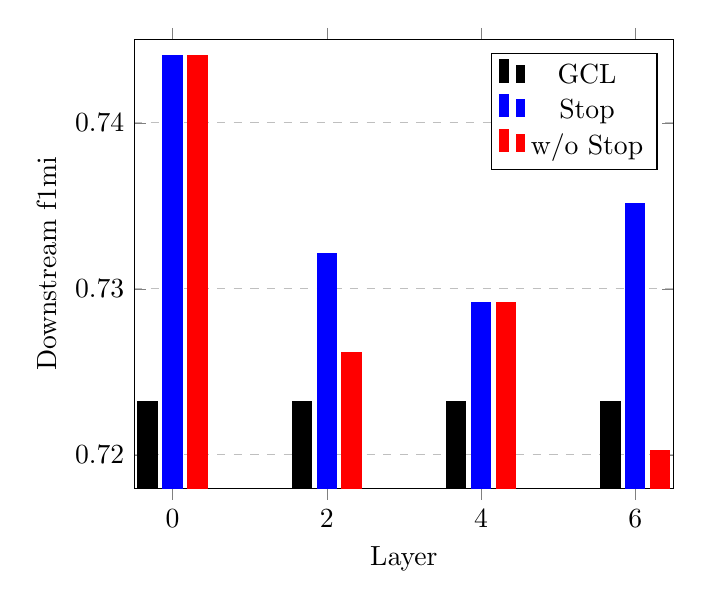
\begin{tikzpicture}
\begin{axis}[
    %title={Temperature dependence of CuSO\(_4\cdot\)5H\(_2\)O solubility},
    % width=0.8\textwidth,
    % height=0.5\textwidth,
    xlabel={Layer},
    ylabel={Downstream f1mi},
    xmin=-0.5, xmax=6.5,
    ymin=0.718, ymax=0.745,
    xtick={-1,0,2,4,6,7}, %,11,12,13},
    ytick={0.69,0.70,0.71,0.72,0.73,0.74,0.75,0.76,0.77,0.78,0.79,0.80,0.81,0.82,0.83}, %57, 58, 59, 60, 61, 62, 63, 64, 65},
    %ytick={0,0.2,0.4,0.6,0.8,1.0}, %,0.6,0.7,0.8,0.9,1.0},
    legend pos=north east,
    ymajorgrids=true,
    grid style=dashed,
    ybar, % Enable bar plots
    bar width=7pt, % Adjust the bar width as needed
]
\addplot+[color=black, % mark=none, error bars/.cd, y dir=both, y explicit, 
    ] coordinates {
    (0, 0.7232142686843872) % +- 0.014580289135568155
    (2, 0.7232142686843872)
    (4, 0.7232142686843872)
    (6,0.7232142686843872)
    };
    \addlegendentry{GCL}

    
\addplot+[color=blue, % mark=square, error bars/.cd, y dir=both, y explicit, 
    ] coordinates {
    (0, 0.7440476218859354)
    (2, 0.7321428656578064)
    (4, 0.7291666666666666)
    (6, 0.7351190249125162)
    };
    \addlegendentry{Stop}
    
\addplot+[color=red, % mark=triangle, error bars/.cd, y dir=both, y explicit, 
    ] 
    coordinates {
    (0, 0.7440476218859354)
    (2, 0.7261904875437418)
    (4, 0.7291666666666666)
    (6, 0.7202380895614624)
    };
    \addlegendentry{w/o Stop}
\end{axis}
\end{tikzpicture}
}
\vspace{-.2in}
%\caption{Continue CIFAR100-CIFAR100}
\caption{PROTEINS}
\label{fig:graphs-proteins-r}
%\vspace{-0.5cm}
\end{subfigure}
\vspace{-.12in}
\caption{Graphs: Deep Augmentation with PCA\vspace{-.1in}}
\vspace{-.19in}
\label{fig:graphs-PCA-N}
%\vspace{-0.5cm}
\end{figure}


\section{Analysis}
\label{sec:analysis}



Our analysis suggests that Deep Augmentation aids contrastive learning by reducing overfitting and eliminating spurious alignment, while maintaining or enhancing uniformity. This is evident in uniformity and alignment measures and corroborated by CKA analysis, which shows that Deep Augmentation decreases similarity between network layers through stronger feature transformations, referred to as reduced co-adaptation between layers. Additionally, the CKA analysis identifies which layers are most susceptible to co-adaptation and where Deep Augmentation is most effective.

% Our analysis suggests that Deep Augmentation helps contrastive learning because it reduces overfitting and removes spurious alignment while maintaining or even improving uniformity. This can be seen in uniformity and alignment measures but is also reflected in CKA analysis, where Deep Augmentation decreases similarity between network layers via stronger transformation of features, i.e. which we refer to as reduced co-adaptation between layers. The added benefit of the CKA analysis is that it locates what layers are most susceptible to this co-adaptation and where Deep Augmentation is most effective.

In contrast, our analysis indicates that Deep Augmentation does not benefit supervised learning because the ground truth labels inherently counteract the spurious alignment present in contrastive learning. In supervised learning, the task is fundamentally different, with ground truth invariances already specified, whereas in contrastive learning, we optimize mutual information across an infinite number of augmentations and invariances. This results in supervised learning exhibiting less co-adaptation between layers. This observation may be analogous to the information bottlenecks seen in supervised versus self-supervised settings \citep{tishby2015deep, shwartzziv2023compress, jing2022understandingCollapse}.

% In contrast, analysis suggests that Deep Augmentation does not help supervised learning because the ground truth labels already counteract the spurious alignment occurring in contrastive learning. Indeed, in supervised learning the task is fundamentally different and the desired invariances already known, while in contrastive learning we optimize mutual information between an infinite number of augmentations and invariances. We can see that supervised learning suffers less from co-adaptation between layers. This may be analogous observation to that of information bottlenecks in supervised versus self-supervised settings  \citep{tishby2015deep, shwartzziv2023compress, jing2022understandingCollapse}.

% -----

% Our analysis suggests that Deep Augmentation mitigates the co-adaptation or ``collapse'' of layers in neural networks trained using contrastive learning. As demonstrated empirically by \citet{Siamese}, stop-gradient is effective in preventing collapse. Similarly, our findings indicate that Deep Augmentation may also prevent collapse, particularly in preventing layers from becoming similar. The most compelling evidence of this effect is in our sentence embeddings experiments. Here, Deep Augmentation, both with and without stop-gradient, appears to counteract layer collapse and influence the overall latent representation. Indeed, Deep Augmentation tends to enhance uniformity, occasionally at the expense of alignment. 

% %This suggests using the CKA similarity index to identify the layer most vulnerable to ``collapse'' and to be targeted by Deep Augmentation. 
% This suggest using the CKA similarity index to identify the layer most vulnerable to ``collapse,'' which should then be the target of Deep Augmentation. Moreover, mitigating information collapse may elucidate adverse impacts of Deep Augmentation in supervised learning, where such collapse could be advantageous in the presence of downstream ground truth labels, unlike in contrastive learning \citep{tishby2015deep, shwartzziv2023compress, jing2022understandingCollapse}.


\subsection{Co-adaptation between Layers}
\label{sec:Co-adaptation-between-Layers}

%\subsubsection{Images and ResNet}





\begin{figure*}[ht]
\centering
\includegraphics[width=0.99\linewidth]{images/simcse_barsf.pdf}\vspace{-.05in}
\caption{CKA similarity index for ``BERT,'' ``SimCSE,'' ``Layer 10 without Stop'' (Deep Augmentation applied without stop-gradient at Layer 10), and ``Layer 8 with Stop'' (Deep Augmentation applied with stop-gradient at Layer 8) on the STS-B dataset. Black crosses mark the beginning and end of a co-adaptation region in BERT, while red crosses on ``Layer 10 without Stop'' and ``Layer 8 with Stop'' highlight the targets of Deep Augmentation. Optimal performance of Deep Augmentation is observed near the black crosses, indicating its effectiveness and guiding the selection of layers for targeting.\vspace{-.1in}}
% \caption{CKA similarity index for ``BERT'', ``SimCSE'', ``Layer 10 without Stop'' (Deep Augmentation without stop-gradient at Layer 10), and ``Layer 8 with Stop'' (Deep Augmentation with stop-gradient at Layer 8) on STS-B. Black crosses indicate start and end of a co-adaptation region in BERT, and red crosses in ``Layer 10 without Stop'' and ``Layer 8 with Stop'' indicate Deep Augmentation's targets. The layers at which Deep Augmentation performs best are around the black crosses at the initialization ``BERT''. CKA demonstrates the effects of Deep Augmentation as well as suggests layers to target.\vspace{-.1in}}
\label{fig:simcse_bars}
\end{figure*}

\textbf{Sentence Embeddings and Transformer.}
We compute the CKA similarity index for the Transformer trained under various settings (Figure \ref{fig:simcse_bars}). ``BERT'' is the starting point for both SimCSE and Deep Augmentation.``BERT'' has a stretch of co-adaptation between layers 8 through 11 as indicated by the two black crosses. Mirroring ResNet18 on CIFAR, it is around these two crosses that Deep Augmentation is most effective, with stop-gradient at the earlier cross and without stop-gradient at the later cross. ``SimCSE'' reduces the co-adaptation across layers, especially between layers 11-10-12. In ``Layer 10 without Stop'' and ``Layer 8 with Stop'' the red cross indicates where Deep Augmentation was applied. ``Layer 10 without Stop'' and ``Layer 8 with Stop'' supersede SimCSE in reducing co-adaptation among the layers following their application. Thus, CKA similarity index highlights a co-adaptation issue between layers and determines at what layer Deep Augmentation should be applied. Future work may investigate if simultaneously targeting multiple layers further improves performance.

In Figure \ref{fig:supervised-simcse-cka} in the Appendix, we note that the supervised setting exhibits significantly reduced co-adaptation even in the absence of Deep Augmentation, indicating this issue is less pronounced in such contexts. Further details are provided in Appendix \ref{appendix:supervised-CKA-simcse}. %\ref{appendix:CKA}.

% In Appendix \ref{appendix:sentence-supervised-cka}, we observe that in the supervised setting, there is significantly less co-adaption already without Deep Augmentation, suggesting it is less of a problem there. See Appendix \ref{appendix:sentence-supervised-cka} for more details.

% serves as a pathology 

%Further trying to understand why Deep Augmentation works and on what layers 

% We apply centered kernel alignment (CKA) \citep{CKAsimilarity} to measure layer similarity between NN layers. Figure \ref{figure:barsresnet18} displays CKA results for a ResNet18 initially random, then trained with SimCLR, and finally with Deep Augmentation excluding stop-gradient after Layer 4. Additional configurations are detailed in the Appendix, typically aligning with ''SimCLR'' or ''Layer 4 without Stop'' patterns. Training with SimCLR reveals co-adaptation between Layers 4 and 5, absent in initial states, with ''Layer 4 without Stop'' showing increased co-adaptation, particularly for underperforming Layer 5. Conversely, optimal Layers 4 and 6 resemble ''SimCLR,'' indicating co-adaptation as a potential failure mode, especially between Layer 4 and subsequent layers in ResNet18. Deep Augmentation influences this co-adaptation, suggesting that finer augmentation granularity could promote more distinct layer functions.

%We use the centered kernel alignment (CKA) \citep{CKAsimilarity} as a similarity index between layers across a NN. 

\textbf{Images and ResNet.}
Figure \ref{figure:barsresnet18} shows CKA for a randomly-initialized ResNet18, after training with SimCLR and after trainining with Deep Augmentation without stop-gradient post-Layer 4. We include results for more settings in the Appendix, but most resemble ``SimCLR'' or ``Layer 4 without Stop.'' There is strong co-adaptation between Layer 4 and 5 after training with SimCLR but not before, and poorly performing ``Layer 4 without Stop'' has increased co-adaptation between Layer 4 and 5. In contrast, top performing Layer 4 and 6 are similar to ``SimCLR.'' This suggests a failure case involving increased co-adaptation between layers, and that Layer 4 is special because ResNet18 is susceptible to co-adaptation between Layer 4 and subsequent layers. 
This also pinpoints where Deep Augmentation is most effective, a pattern similarly noted in our sentence embeddings analysis.
%affects co-adaptation between layers, and learning invariances to a greater granularity of augmentations should arguably lead to more specialized layers.

 %(which is also true for poorly performing Layer 5 in the Appendix)


 In Figure \ref{fig:appendix-supervised-CIFAR-cka} in the Appendix, we observe that the supervised setting exhibits reduced co-adaptation compared to the self-supervised settings, particularly in the last layer. This consistent difference, as also observed with sentence embeddings, underscores a disparity between self-supervised and supervised learning.

 % In Figure \ref{} in the Appendix, we observe that in the supervised setting there is reduced co-adaptation compared to the self-supervised settings, especially for the last layer. Again, as with sentence embeddings, this shows that a consistent difference between self-supervised and supervised learning. 


\begin{figure}[ht]
\centering
\includegraphics[width=0.8\linewidth]{images/Bars1f.pdf}\vspace{-.05in}
\caption{Indications of why Layer 4 is special in Figure~\protect\ref{fig:CIFAR100-CIFAR100-stop-vs-not-N}, as the major divide between co-adaptation across layers. Layers 0-4 are convolutional. All high-performing NNs have the pattern of SimCLR, and failure cases have stronger co-adaptation between Layers 4 and 5. ``Layer 4 without Stop'' corresponds to the failure case of Deep Augmentation without stop-gradient at Layer 4. }
\label{figure:barsresnet18}
\vspace{-.1in}
\end{figure}

%\subsubsection{Sentence Embeddings and Transformer}

\subsection{Alignment and Uniformity}
\label{sec:alignment-uniformity}



% \subsubsection{Sentence Embeddings and Transformer}
% \label{sec:alignment-uniformity-text}
\textbf{Sentence Embeddings and Transformer.}
% (which were  also used to characterize SimCSE when it was introduced)
Alignment and Uniformity measures for sentence embedding methods are in Figure \ref{fig:align_uniform_simcse}, computed as in SimCSE \citep{gao-etal-2021-simcse} w.r.t.\ ground truth (STS-B development set), during training, and with methods converging to higher density regions.  

\begin{figure}[ht]
\centering
\resizebox{0.5\columnwidth}{!}{%
\begin{tikzpicture}
\begin{axis}[
    enlargelimits=true,
    grid style=dashed,
    xlabel={Uniformity},
    ylabel={Alignment},
    % xtick={-2.77, -2.76, -2.75, -2.74, -2.73, -2.72}, %,11,12,13},
    % ytick={1.99, 2},
]

\addplot[
    color=black,
    only marks,
    mark=o,
    mark size=2.9pt
] table [x expr=\thisrowno{1},y expr=\thisrowno{0}] {data2/rep_best.txt};
\addlegendentry{SimCSE}
\addplot[
    color=blue,
    only marks,
    %scatter,
    mark=square,
    mark size=2.9pt
] table [x expr=\thisrowno{1},y expr=\thisrowno{0}] {data2/reg_best.txt};
\addlegendentry{S}
% \addplot[
%     color=blue,
%     only marks,
%     %scatter,
%     mark=square,
%     mark size=2.9pt]
% table[meta=Uniformity]
% {data2/reg_best.txt};
% \addlegendentry{L4}
\addplot[
    color=orange,
    only marks,
    %scatter,
    mark=pentagon,
    mark size=2.9pt
] table [x expr=\thisrowno{1},y expr=\thisrowno{0}] {data2/train_best.txt};
\addlegendentry{w/o S}
\addplot[
    color=red,
    only marks,
    %scatter,
    mark=triangle,
    mark size=2.9pt
] table [x expr=\thisrowno{1},y expr=\thisrowno{0}] {data2/BestREPMLM.txt};
\addlegendentry{SimCSE+MLM}
\addplot[
    color=yellow,
    only marks,
    %scatter,
    mark=o,
    mark size=2.9pt
] table [x expr=\thisrowno{1},y expr=\thisrowno{0}] {data2/REGbestMLM.txt};
\addlegendentry{S+MLM}
\addplot[
    color=green,
    only marks,
    %scatter,
    mark=triangle,
    mark size=2.9pt
] table [x expr=\thisrowno{1},y expr=\thisrowno{0}] {data2/TMLMBEST.txt};
\addlegendentry{w/o S+MLM}


% \draw[->] (A) -- (B) node[midway,fill=white] {\emph{success}};

\coordinate (o2) at (axis cs:-2.48,0.54);
\coordinate (o1) at (axis cs:-2.4,0.46);
\draw [->,orange](o1) -- (o2);
\coordinate (g1) at (axis cs:-2.40,0.44);
\coordinate (g2) at (axis cs:-2.355,0.412);
\draw [->,green](g1) -- (g2);
\coordinate (b1) at (axis cs:-2.269,0.429);
\coordinate (b2) at (axis cs:-2.333,0.47);
\draw [->,blue](b1) -- (b2);
\coordinate (s1) at (axis cs:-2.14,0.43);
\coordinate (s2) at (axis cs:-2.2,0.47);
\draw [->,black](s1) -- (s2);
\coordinate (r1) at (axis cs:-2.08,0.403);
\coordinate (r2) at (axis cs:-1.92,0.34);
\draw [->,red](r1) -- (r2);
\coordinate (y1) at (axis cs:-2.15,0.39);
\coordinate (y2) at (axis cs:-2.01,0.33);
\draw [->,yellow](y1) -- (y2);

%\draw[->,red] (3,3) -- ( $ (a)!.25!(0,0) $ ) node [midway, sloped, above] {12 m/s};

% \coordinate (a) at (3,3);
% \coordinate (b) at (3,0);
% \coordinate (c) at (-3,3);
% \node (O) at (0,0) {origin};
% \draw[->,red] (3,3) -- ( $ (a)!.25!(0,0) $ ) node [midway, sloped, above] {12 m/s};
% \draw[->,blue] (b) -- ( $ (b)!.8!(0,0) $ ) node [midway, sloped, above] {12 m/s};
% \draw[->,magenta] (c) -- ( $ (c)!.5!(0,0) $ ) node [midway, sloped, above] {12 m/s};

\end{axis}
\end{tikzpicture}
}\vspace{-.05in}
\caption{Alignment and Uniformity (lower is better) for sentence embeddings on STS-B: SimCSE vs.\ Deep Augmentation (with and without stop-gradient). We also include these methods combined with the pre-training method of BERT, i.e., Masked Language Modeling (MLM). Arrows indicate the direction during training, which  reverses when MLM is introduced. ``S'' is short for stop-gradient.}
\label{fig:align_uniform_simcse}
\vspace{-.1in}
\end{figure}

Without MLM, all methods converge toward better Uniformity at the expense of Alignment. ``S'' is consistently better in both measures than ``SimCSE,'' while ``w/o S'' further encourages Uniformity at the expense of Alignment. With MLM, the direction reverses, and all methods improve Alignment. Again ``S+mlm'' (MLM and Deep Augmentation with stop-gradient) is consistently better than ``SimCSE+mlm'' in both Alignment and Uniformity. ``w/o S+mlm'' (MLM and Deep Augmentation without stop-gradient) achieves markedly improved Uniformity compared to ''SimCSE+mlm,'' albeit at the cost of Alignment.

This suggests that Deep Augmentation generally achieves better Alignment and Uniformity than SimCSE, particularly in terms of Uniformity. This analysis is consistent with that of SimCSE  \cite{gao-etal-2021-simcse}. However, since these measures are computed on ground truth validation classes rather than augmentations, they offer a different perspective from the original introduction of these measures for contrastive learning \cite{wang2020hypersphere}.

In Table \ref{appendix:supervised-CKA-simcse} in the Appendix, we present Alignment and Uniformity metrics for supervised learning on the same validation ground truth classes. The results indicate that Deep Augmentation achieves better Alignment but worse Uniformity. Notably, Uniformity is already higher for regular supervised learning compared to self-supervised approaches, and Deep Augmentation does not improve this metric.

% In Table \ref{appendix:supervised-CKA-simcse} in the Appendix, we include also include Alignment and Uniformity for supervised learning on the same validation ground truth classes. There we can see that Deep Augmentation achieve better Alignment but worse Uniformity. The Uniformity is already higher for Regular supervised learning than any of the self-supervised approaches, and Deep Augmentation does not add value here.

% This suggests that Deep Augmentation generally achieves better Alignment and Uniformity then SimCSE, especially in terms of Uniformity. This is a congruous analysis with that in the SimCSE work \cite{gao-etal-2021-simcse}; However, given that these measures are computed on ground truth validation data rather then on augmentations, they tell a different story than how these measures were originally introduced for constrastive learning \cite{wang2020hypersphere}.

% This suggests that Deep Augmentation effectively mitigates collapse or ``non-uniformity'' in the latent space, complementing MLM's propensity for such collapse.

% ``w/o S+mlm'' (MLM and Deep Augmentation witout stop-gradient) acheives substantially better Uniformity than  ``SimCSE+mlm'' at the expense of Alignment. This indicates that Deep Augmentation is especially suited at counteracting collapse in the latent space, making it a good compliment to MLM that has more collapsing tendencies. 

%On the contrary, ``w/o S+mlm'' (the same without stop-gradient) is below ``S'' and ``SimCSE'' in both Alignment and Uniformity, but performs worse on downstream tasks, indicating that these measures do not paint a complete picture. %This may be due to STS-Benchmark set is a development set and thus merely a useful proxy.

% \subsubsection{Images and ResNet}
% \label{sec:alignment-uniformity-images}
\textbf{Images and ResNet.}
The Alignment/Uniformity measures depend on specific augmentations. Our approach, involving different augmentations, complicates direct comparison, so we standardized using SimCLR's data augmentations (Figure \ref{fig:align_uniform}). Analysis over five checkpoints (epochs 300, 600, 900, 1200, 1500) shows more training generally improves Uniformity on test data and Alignment on training data.

Layers 4 and 6 with stop-gradient outperform in Alignment and Uniformity using SimCLR augmentations on test data, and in Uniformity on the training data. Conversely, Layer 4 without stop-gradient and SimCLR exhibit better Alignment on training data, suggesting potential overfitting of Alignment as their test set Alignment degrades with training. Layer 5 performs poorly in both sets, aligning with downstream results. Despite differences in downstream tasks, SimCLR and Layer 4 without stop-gradient have similar Alignment and Uniformity, highlighting these metrics' limitations in capturing latent space quality. Hence, our preference for the CKA similarity index for comprehensive assessment.

In Figure \ref{fig:appendix-supervised-align_uniform} in the Appendix, we present the Alignment and Uniformity metrics for supervised models trained on ground truth labels. While no overfitting is observed, Layers 4 with stop-gradient again perform better on both metrics. This highlights that the invariances in self-supervised learning and supervised learning remain fundamentally different, and superior performance in the self-supervised task does not necessarily translate to improved performance in the supervised downstream task. Avoiding overfitting to Alignment is crucial when that Alignment differs from the ground truth, but less critical when Alignment matches the ground truth.

% In Figure \ref{} in Appendix, we include the same Alignment and Uniformity metrics but for supervised models trained on ground truth labels. While there is no overfitting, we can again see that Layers 4 with stop-gradient performs better on both metrics. This reinforces the fact that invariances in self-supervised learning and supervised learning are still fundamental different, and that better performance on the self-supervised task does not necessarily translate to better performance on the supervised downstream task. Not overfitting to Alignment is extra important when that Alignment is different from the ground truth, but less so when the Alignment is the ground truth.

% We apply the Alignment and Uniformity measures \citep{wang2020hypersphere} to assess the quality of representations. However, these measures are defined with respect to a specific set of augmentations. Since we use higher-layer transformations, it is not clear how to compare across our experiments. Thus, we use the SimCLR data transformations across methods; see Figure \ref{fig:align_uniform} for results for five checkpoints (at epochs 300, 600, 900, 1200, 1500) per method. For each method, more training leads to better (lower) Uniformity on the test data, while Alignment improves with more training on the training data.

% On the test set, Layer 4 and 6 (both with stop-gradient) achieve better Alignment and Uniformity with respect to the SimCLR data augmentations. The measures on the training data show that Layer 4 and 6, with stop-gradient, achieve better Uniformity. On the other hand, Layer 4 without stop-gradient and SimCLR achieves stronger Alignment---hence overfitting to the training set as Alignment on the test set worsens during training. Layer 5's measures are worse on both the training and test set, in accordance with its downstream performance. However, even though SimCLR and Layer 4 without stop-gradient perform substantially different on the downstream task, their Alignment and Uniformity are surprisingly similar, indicating that Alignment and Uniformity do not provide a complete picture. Indeed, relying on measures defined with respect to a specific augmentation, to assess the quality of a latent space is insufficient, which is why we prefer the CKA similarity index.

\begin{figure}[ht]
\centering
\resizebox{0.8\columnwidth}{!}{%
\begin{tikzpicture}
\begin{axis}[
    enlargelimits=true,
    grid style=dashed,
    xlabel={Uniformity},
    ylabel={Alignment},
    legend pos=south east,
    % xtick={-2.77, -2.76, -2.75, -2.74, -2.73, -2.72}, %,11,12,13},
    % ytick={1.99, 2},
]
\addplot[
    color=black,
    only marks,
    mark=o,
    mark size=2.9pt]
table[meta=Alignment]
{data/scattered_simclr100.dat};
\addlegendentry{SimCLR}
\addplot[
    color=blue,
    only marks,
    %scatter,
    mark=square,
    mark size=2.9pt]
table[meta=Alignment]
{data/scattered_a100l4.dat};
\addlegendentry{L4 w/ S}
\addplot[
    color=orange,
    only marks,
    %scatter,
    mark=pentagon,
    mark size=2.9pt]
table[meta=Alignment]
{data/scattered_at100l4.dat};
\addlegendentry{L4 w/o S}
\addplot[
    color=red,
    only marks,
    %scatter,
    mark=diamond,
    mark size=2.9pt]
table[meta=Alignment]
{data/scattered_a100l5.dat};
\addlegendentry{L5 w/ S}
\addplot[
    color=green,
    only marks,
    %scatter,
    mark=triangle,
    mark size=2.9pt]
table[meta=Alignment]
{data/scattered_a100l6.dat};
\addlegendentry{L6 w/ S}

\coordinate (a1) at (axis cs:-2.725,0.3);
\coordinate (a2) at (axis cs:-2.75,0.3);
\draw[->] (a1) -- (a2) node[midway,fill=white] {\emph{training}};

\end{axis}
\end{tikzpicture}
% \caption{Alignment and Uniformity}
% \label{fig:align_uniform}
% \end{figure}

% \begin{figure}[ht]
\begin{tikzpicture}
\begin{axis}[
    enlargelimits=true,
    grid style=dashed,
    xlabel={Uniformity},
    ylabel={Alignment},
    legend pos=south east,
    % xtick={-2.77, -2.76, -2.75, -2.74, -2.73, -2.72}, %,11,12,13},
    % ytick={1.99, 2},
]
\addplot[
    color=black,
    only marks,
    mark=o,
    mark size=2.9pt]
table[meta=Alignment]
{data_train/scattered_simclr100.dat};
\addlegendentry{SimCLR}
\addplot[
    color=blue,
    only marks,
    %scatter,
    mark=square,
    mark size=2.9pt]
table[meta=Alignment]
{data_train/scattered_a100l4.dat};
\addlegendentry{L4 w/ S}
\addplot[
    color=orange,
    only marks,
    %scatter,
    mark=pentagon,
    mark size=2.9pt]
table[meta=Alignment]
{data_train/scattered_at100l4.dat};
\addlegendentry{L4 w/o S}
\addplot[
    color=red,
    only marks,
    %scatter,
    mark=diamond,
    mark size=2.9pt]
table[meta=Alignment]
{data_train/scattered_a100l5.dat};
\addlegendentry{L5 w/ S}
\addplot[
    color=green,
    only marks,
    %scatter,
    mark=triangle,
    mark size=2.9pt]
table[meta=Alignment]
{data_train/scattered_a100l6.dat};
\addlegendentry{L6 w/ S}

% \draw[->] (A) -- (B) node[midway,fill=white] {\emph{success}};

\coordinate (a1) at (axis cs:-2.768,0.265);
\coordinate (a2) at (axis cs:-2.768,0.188);
\draw[->] (a1) -- (a2) node[midway,fill=white] {\emph{training}};

\end{axis}
\end{tikzpicture}
}
\vspace{-.1in}
\caption{Alignment and Uniformity (lower is better) of SimCLR augmentations on CIFAR. Left: Test data. Right: Training data. Deep Augmentation outperforms SimCLR when measuring alignment and uniformity \emph{using SimCLR's augmentations} on the test set, and SimCLR overfits at Alignment on the training set. ``L'' is short for Layer and ``S'' is short for stop-gradient. \vspace{-.1in}}
\label{fig:align_uniform}
\end{figure}







\section{Discussion}

% We studied higher layer transformations for enhanced self-supervised learning. Our findings demonstrate that this approach is effective when applied to both image-based contrastive learning using a ResNet architecture and sentence embedding generation using a Transformer model. We also examined the use of stop-gradient operations as well as the relationship between traditional input data transformations and higher layer transformations. Finally, we provided an interpretation of our approach as alleviating co-adaptation between layers.

This paper presents the multifaceted impacts of Deep Augmentation techniques on contrastive and supervised learning. We demonstrate the efficacy of layer-targeted dropout, both with and without stop-gradient, in enhancing contrastive learning across  modalities. This effect is most pronounced in higher layers, underscoring the importance of strategic layer selection in augmentation techniques. Contrastingly, our investigation into supervised learning contexts reveals an inverse relationship. 
%suggesting that phenomena akin to ``collapse'' may benefit direct training on downstream tasks.

Furthermore, we introduce another modality-agnostic PCA-based augmentation strategy, demonstrating its use as an alternative to dropout. This approach not only mirrors performance enhancements attributed to dropout but also provides a versatile tool applicable across learning scenarios.

Our findings address the issue of co-adaptation among network layers and their latent features. Our targeting of specific layers underscores the potential of informed, strategic interventions in network training. While much future work is needed to fully understand the mechanisms of self-supervised learning, our analysis indicates that Deep Augmentation aids contrastive learning by reducing overfitting and eliminating spurious alignments, while maintaining or even enhancing uniformity.

Extensive ablation studies underpin our contributions, providing a robust empirical foundation. These pave the way for future research to explore the interplay between augmentation techniques, network architectures, and learning paradigms, with the ultimate goal of enhancing machine learning models' efficiency and versatility.

%\flushcolsend
%\clearpage
% \section*{Impact Statement}
% This paper presents work whose goal is to advance machine learning. There are no societal consequences of our work that we feel must be specifically highlighted here.

%{\small
%\bibliographystyle{ieee_fullname}
%\bibliography{example_paper}
\bibliographystyle{tmlr}
\bibliography{egbib}
%}


% \clearpage
% \newpage
% \appendix

\clearpage
\newpage
\appendix
%\onecolumn

%%%%%%%%%%%%%%%%%%%%%%%%%%%%%%%%%%%%%%%%%%%%%%
%%%%%%%%%%%%%%%%%%%%%%%%%%%%%%%%%%%%%%%%%%%%%%
%%%%%%%%%%%%%%%%%%%%%%%%%%%%%%%%%%%%%%%%%%%%%%
%%%%%%%%%%%%%%%%%%%%%%%%%%%%%%%%%%%%%%%%%%%%%%
%%%%%%%%%%%%%%%%%%%%%%%%%%%%%%%%%%%%%%%%%%%%%%
%%%%%%%%%%%%%%%%%%%%%%%%%%%%%%%%%%%%%%%%%%%%%%
%%%%%%%%%%%%%%%%%%%%%%%%%%%%%%%%%%%%%%%%%%%%%%
%%%%%%%%%%%%%%%%%%%%%%%%%%%%%%%%%%%%%%%%%%%%%%
%%%%%%%%%%%%%%%%%%%%%%%%%%%%%%%%%%%%%%%%%%%%%%
%%%%%%%%%%%%%%%%%%%%%%%%%%%%%%%%%%%%%%%%%%%%%%
%%%%%%%%%%%%%%%%%%%%%%%%%%%%%%%%%%%%%%%%%%%%%%
%%%%%%%%%%%%%%%%%%%%%%%%%%%%%%%%%%%%%%%%%%%%%%
%%%%%%%%%%%%%%%%%%%%%%%%%%%%%%%%%%%%%%%%%%%%%%
%%%%%%%%%%%%%%%%%%%%%%%%%%%%%%%%%%%%%%%%%%%%%%
%%%%%%%%%%%%%%%%%%%%%%%%%%%%%%%%%%%%%%%%%%%%%%
%%%%%%%%%%%%%%%%%%%%%%%%%%%%%%%%%%%%%%%%%%%%%%
%%%%%%%%%      APPENDIX
%%%%%%%%%%%%%%%%%%%%%%%%%%%%%%%%%%%%%%%%%%%%%%
%%%%%%%%%%%%%%%%%%%%%%%%%%%%%%%%%%%%%%%%%%%%%%
%%%%%%%%%%%%%%%%%%%%%%%%%%%%%%%%%%%%%%%%%%%%%%
%%%%%%%%%%%%%%%%%%%%%%%%%%%%%%%%%%%%%%%%%%%%%%
%%%%%%%%%%%%%%%%%%%%%%%%%%%%%%%%%%%%%%%%%%%%%%
%%%%%%%%%%%%%%%%%%%%%%%%%%%%%%%%%%%%%%%%%%%%%%
%%%%%%%%%%%%%%%%%%%%%%%%%%%%%%%%%%%%%%%%%%%%%%
%%%%%%%%%%%%%%%%%%%%%%%%%%%%%%%%%%%%%%%%%%%%%%
%%%%%%%%%%%%%%%%%%%%%%%%%%%%%%%%%%%%%%%%%%%%%%
%%%%%%%%%%%%%%%%%%%%%%%%%%%%%%%%%%%%%%%%%%%%%%
%%%%%%%%%%%%%%%%%%%%%%%%%%%%%%%%%%%%%%%%%%%%%%
%%%%%%%%%%%%%%%%%%%%%%%%%%%%%%%%%%%%%%%%%%%%%%
%%%%%%%%%%%%%%%%%%%%%%%%%%%%%%%%%%%%%%%%%%%%%%
%%%%%%%%%%%%%%%%%%%%%%%%%%%%%%%%%%%%%%%%%%%%%%
%%%%%%%%%%%%%%%%%%%%%%%%%%%%%%%%%%%%%%%%%%%%%%
%%%%%%%%%%%%%%%%%%%%%%%%%%%%%%%%%%%%%%%%%%%%%%





\section{CIFAR}
\label{appendix:vision}

In this section, we outline the training specifics for our experiments on the CIFAR datasets, complemented by supplementary results and comparative analyses.

\subsection{ResNet architecture}
\label{appendix:resnetarch}

The specifications for ResNet18 are detailed in Table \ref{table:resnet18-N}.

\begin{table}[ht] % [H]
\caption{Configuration of ResNet18 on CIFAR}
\centering
\begin{tabular}{ |p{0.7cm}||p{2.4cm}|p{2.8cm}|  }
 \hline
 \multicolumn{3}{|c|}{ResNet18 on CIFAR} \\
 \hline
 Layer & Type & \#Neurons  \\
 \hline
 -1    & Input Data        & $32^2\times3=3072$      \\
 0     & Conv(k=3, s=1)    & $32^2\times64=65536$    \\
 1     & Conv(k=3, s=2)    & $32^2\times64=65536$    \\
 2     & Conv(k=3, s=2)    & $16^2\times128=32768$   \\
 3     & Conv(k=3, s=2)    & $8^2\times256=16384$    \\
 4     & Conv(k=3, s=2)    & $4^2\times512=8192$     \\
 5     & Avgpool           & $512$                  \\
 6     & MLP               & $128$                  \\
 \hline
\end{tabular}
\label{table:resnet18-N}
\end{table}

\subsection{Proportion of Dropped Nodes}
\label{appenxix:ratio}

When setting a dropout rate for a specific layer, it exclusively affects that layer. Consequently, a 50\% dropout rate at one layer results in fewer neurons being dropped compared to a 50\% dropout applied uniformly across all layers. Additionally, the same dropout rate can impact different numbers of neurons in various layers, reflecting the varying neuron counts in each layer.

In Table \ref{tab:dropped_nodes} we include the number of nodes in each layer, the total nodes across all layers. Thus, for $0.5$ dropout, we show the proportion of dropped nodes when a layer is targeted. There is not trend between the proportion and performance.
\begin{table}[ht]
\centering
\caption{Proportion of Dropped Nodes per Layer at 50\% dropout}
\label{tab:dropped_nodes}
\begin{tabular}{@{}cccc@{}}
\toprule
Layer & Dropped Nodes & Total Nodes & Proportion \\ \midrule
0     & $0.5 \times 65536$   & 192640      & 0.17                                   \\
1     & $0.5 \times 65536$   & 192640      & 0.17                                   \\
2     & $0.5 \times 32768$   & 192640      & 0.085                                  \\
3     & $0.5 \times 16384$   & 192640      & 0.043                                  \\
4     & $0.5 \times 8192$    & 192640      & 0.021                                  \\
5     & $0.5 \times 512$     & 192640      & 0.001                                  \\
6     & $0.5 \times 128$     & 192640      & 0.0003                                 \\ \bottomrule
\end{tabular}
\end{table}


\subsection{Training Details}

For implementation, we utilized the code provided by \citep{supcontrast}, available at \href{https://github.com/HobbitLong/SupContrast}{this link}. Our experiments were conducted with a batch size of 1024, training each method for 1500 epochs.

% We used the code released by \citep{supcontrast} at \href{https://github.com/HobbitLong/SupContrast}{link}. We used a batch-size of 1024 and trained each method for 1500 epochs. 

%\subsection{Dropout-rates: Layer vs. Neurons}



\subsection{Na\"ive Deep Augmentation with stop-gradient on CIFAR100}
\label{appendix:naive-stopgradient}

% Initially, the stop-gradient operation was uniformly applied to all samples in the batch, resulting in the exclusion of training for layers up to and including the targeted layer. The outcomes of this approach, detailed in the Appendix, were predictably suboptimal

In Figure \ref{fig:two-sided-dropout-CIFAR100-CIFAR100}, we include results of 50\% dropout with stop-gradient at individual layers on 100\% of the batch. Such na\"ive augmentations generally give poor performances. All layers besides the input data layer lead to downstream accuracy of 1\% (equivalent with random guess). The input data layer arrives at a downstream accuracy of 61.38\%. 

\begin{figure}[ht]
\centering
\resizebox{0.33\columnwidth}{!}{%
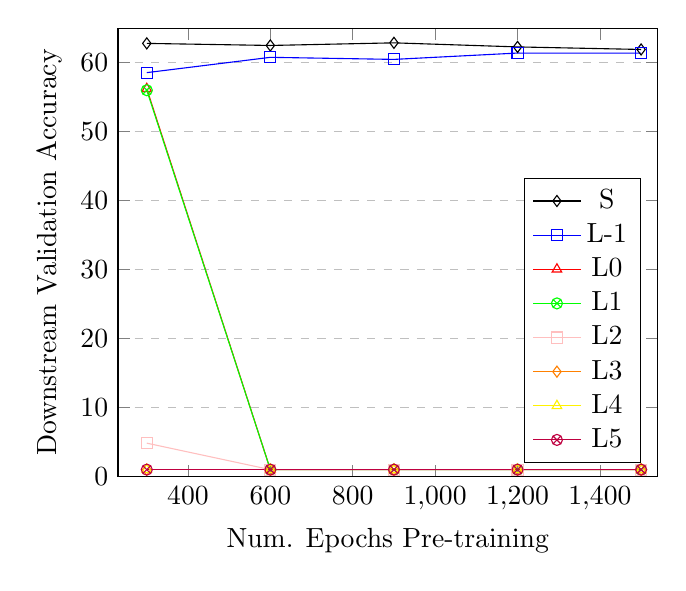
\begin{tikzpicture}
\begin{axis}[
    %title={Temperature dependence of CuSO\(_4\cdot\)5H\(_2\)O solubility},
    % width=0.8\textwidth,
    % height=0.5\textwidth,
    xlabel={Num. Epochs Pre-training},
    ylabel={Downstream Validation Accuracy},
    xmin=230, xmax=1540,
    ymin=0, ymax=65,
    xtick={200,400,600,800,1000,1200,1400}, %,11,12,13},
    ytick={0,10, 20, 30, 40, 50, 60},
    %ytick={0,0.2,0.4,0.6,0.8,1.0}, %,0.6,0.7,0.8,0.9,1.0},
    legend pos=south east,
    ymajorgrids=true,
    grid style=dashed,
]
\addplot[
    color=black,
    mark=diamond,
    ]
    coordinates {
    (300,62.79999923706055)(600,62.5)(900,62.87999725341797)(1200,62.28999710083008)(1500,61.91999816894531)
    };
    \addlegendentry{S}

\addplot[
    color=blue,
    mark=square,
    ]
    coordinates {
    (300,58.55999755859375)(600,60.779998779296875)(900,60.47999954223633)(1200,61.39999771118164)(1500,61.37999725341797)
    };
    \addlegendentry{L-1}
\addplot[
    color=red,
    mark=triangle,
    ]
    coordinates {
    (300,56.21999740600586)(600,1.0)(900,1.0)(1200,1.0)(1500,1.0)
    };
    \addlegendentry{L0}
\addplot[
    color=green,
    mark=otimes,
    ]
    coordinates {
    (300,56.0099983215332)(600,1.0)(900,1.0)(1200,1.0)(1500,1.0)
    };
    \addlegendentry{L1}
\addplot[
    color=pink,
    mark=square,
    ]
    coordinates {
    (300,4.839999675750732)(600,1.0)(900,1.0)(1200,1.0)(1500,1.0)
    };
    \addlegendentry{L2}
\addplot[
    color=orange,
    mark=diamond,
    ]
    coordinates {
    (300,1.0)(600,1.0)(900,1.0)(1200,1.0)(1500,1.0)
    };
    \addlegendentry{L3}
\addplot[
    color=yellow,
    mark=triangle,
    ]
    coordinates {
    (300,1.0)(600,1.0)(900,1.0)(1200,1.0)(1500,1.0)
    };
    \addlegendentry{L4}
\addplot[
    color=purple,
    mark=otimes,
    ]
    coordinates {
    (300,1.0)(600,1.0)(900,1.0)(1200,1.0)(1500,1.0)
    };
    \addlegendentry{L5}

\end{axis}
\end{tikzpicture}
}
%\vspace{-.1in}
\caption{CIFAR100. 50\% dropout with stop-gradient applied at individual layers on 100\% of the batch. I.e. freezing earlier layers to random weights.}
\label{fig:two-sided-dropout-CIFAR100-CIFAR100}
%\vspace{-0.5cm}
\end{figure}

\subsection{Including Deep Augmentation w/o stop gradient initialized with SimCLR}

For completion, we also include Deep Augmentation without stop gradient, initialized with pre-trained SimCLR model, together with the other variants---see Figure \ref{fig:CIFAR100-CIFAR100-stop-vs-not-full}. %We did not include it in the main part because we felt the figure got cluttered.

\begin{figure}[ht]
\centering
\resizebox{0.33\columnwidth}{!}{%
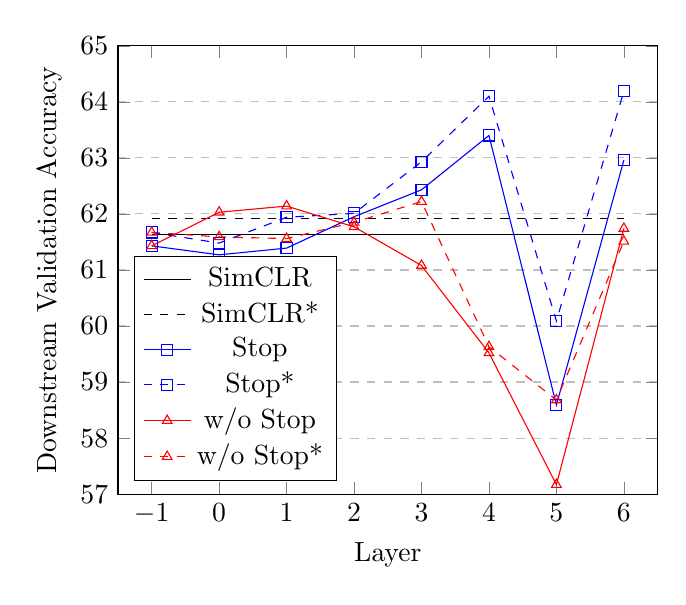
\begin{tikzpicture}
\begin{axis}[
    %title={Temperature dependence of CuSO\(_4\cdot\)5H\(_2\)O solubility},
    % width=0.8\textwidth,
    % height=0.5\textwidth,
    xlabel={Layer},
    ylabel={Downstream Validation Accuracy},
    xmin=-1.5, xmax=6.5,
    ymin=57, ymax=65,
    xtick={-1,0,1,2,3,4,5,6,7}, %,11,12,13},
    ytick={57, 58, 59, 60, 61, 62, 63, 64, 65},
    %ytick={0,0.2,0.4,0.6,0.8,1.0}, %,0.6,0.7,0.8,0.9,1.0},
    legend pos=south west,
    ymajorgrids=true,
    grid style=dashed,
]
\addplot[
    color=black,
    %mark=diamond,
    ]
    coordinates {
    % (300,62.14999771118164)(600,63.15999984741211)(900,62.91999816894531)(1200,62.29999923706055)(1500,61.93000030517578)
    (-1,61.64)
    (0,61.64)
    (1,61.64)
    (2,61.64)
    (3,61.64)
    (4,61.64)
    (5,61.64)
    (6,61.64)
    };
    \addlegendentry{SimCLR}
\addplot[
    %dotted,
    dashed,
    mark options={solid},
    color=black,
    %mark=diamond,
    ]
    coordinates {
    % (300,62.14999771118164)(600,63.15999984741211)(900,62.91999816894531)(1200,62.29999923706055)(1500,61.93000030517578)
    (-1,61.91999816894531)
    (0,61.91999816894531)
    (1,61.91999816894531)
    (2,61.91999816894531)
    (3,61.91999816894531)
    (4,61.91999816894531)
    (5,61.91999816894531)
    (6,61.91999816894531)
    };
    \addlegendentry{SimCLR*}
\addplot[
    color=blue,
    mark=square,
    ]
    coordinates {
    (-1, 61.43000030517578)
    (0, 61.269996643066406) 
    (1, 61.38999938964844)
    (2, 61.94999694824219)
    (3, 62.43000030517578)
    (4, 63.39999771118164)
    (5, 58.59000015258789)
    (6, 62.959999084472656)
    };
    \addlegendentry{Stop}
\addplot[
    dashed,
    mark options={solid},
    color=blue,
    mark=square,
    ]
    coordinates {
    (-1, 61.66999816894531)
    (0, 61.47999954223633)
    (1, 61.939998626708984)
    (2, 62.0099983215332)
    (3, 62.93000030517578)
    (4, 64.0999984741211)
    (5, 60.09000015258789)
    (6, 64.18999481201172)
    };
    \addlegendentry{Stop*}
\addplot[
    color=red,
    mark=triangle,
    ]
    coordinates {
    (-1, 61.43000030517578)
    (0, 62.029998779296875)
    (1, 62.13999938964844)
    (2, 61.769996643066406)
    (3, 61.07999801635742)
    (4, 59.519996643066406)
    (5, 57.16999816894531)
    (6, 61.73999786376953)
    };
    \addlegendentry{w/o Stop}
\addplot[
    dashed,
    mark options={solid},
    color=red,
    mark=triangle,
    ]
    coordinates {
    (-1, 61.66999816894531)
    (0, 61.59000015258789)
    (1, 61.55999755859375)
    (2, 61.849998474121094)
    (3, 62.21999740600586)
    (4, 59.62999725341797)
    (5, 58.68000030517578)
    (6, 61.5099983215332)
    };
    \addlegendentry{w/o Stop*}


\end{axis}
\end{tikzpicture}
}
%\vspace{-.1in}
%\caption{Continue CIFAR100-CIFAR100}
\caption{Comparing sampling 50\% and applying 50\% dropout, with or without stop-gradient. *: initialized with pre-trained SimCLR model. Stop: short for stop-gradient.}
\label{fig:CIFAR100-CIFAR100-stop-vs-not-full}
%\vspace{-0.5cm}
\end{figure}


\subsection{Freezing}
\label{appendix:freezing-layers}

We repeat the experiment with pre-trained initialization but freeze all the layers up to and including the layer at which the targeted transformation occurs; see ``Freeze before'' in Figure \ref{fig:CIFAR100-CIFAR100-freeze}. Compared to not freezing, this strategy gives very different results. In particular, the downstream performance of Layers 3 and 4 is critically reduced. %; note that Layer 6 means freezing the whole NN. 

%We note in Appendix, Layer 1 and Layer 2 performance is significantly improved and show stronger performance than the SimCLR benchmark in earlier epochs until it shows overfitting behavior. This indicates that there is room to learn improved representation by learning invariances of higher layer SimCLR feature spaces. Future work may explore an iterative approach where we incrementally freeze layers, moving one step up at a time.

%\justin{We got here.}


Deep Augmentation after frozen SimCLR layers may not work well due to co-adaptation between neurons, leading to overfitting. Suppose a layer of a NN exhibits strong co-adaptation within several subsets of neurons, i.e., each subset encodes a single data feature. Randomly dropping neurons is unlikely to remove a complete co-adapted subset of neurons. Ideally, features are learned per neuron so dropping any of them provides a complementary view. Alternatively, features might be represented continuously among neurons in a layer such that dropout corresponds to something akin to blurring the feature continuously.
%, again providing complementary rather than supplementary views. 

%{\color{red} 
Because early layers have fewer parameters to distort the input data, such layers may have less co-adaptation.
%---especially in CNNs where there is a strong inductive image-bias. 
This might explain why earlier layers, rather than later layers, perform better when frozen during Deep Augmentation. Similarly, higher layers may benefit from higher dropout rates because they are more susceptible to co-adaptation, explaining why in Figure \ref{fig:CIFAR100-CIFAR100-stop-vs-not-N}, Deep Augmentation in higher layers yields the best downstream performance. %See Appendix \ref{appendix:freezing-layers} for further discussion. 

Reversely, we may freeze the layers following the targeted layer; results are labeled ``Freeze after'' in Figure \ref{fig:CIFAR100-CIFAR100-freeze}. Compared to ``Freeze before'', Layer 3 improves, Layer 5 worsens, while Layer 4 performs similarly. This asserts that later layers, some more than others, benefit from learning to be invariant to Deep Augmentation. 

We see that Deep Augmentation with freezing layers and initialized to SimCLR-model, works better for earlier layers than for later layers. Especially in Figure \ref{fig:freeze-continue-CIFAR100-CIFAR100} and \ref{fig:CIFAR10-freezingbeforeafter-epochs}, we see that earlier layers outperform SimCLR earlier in the training. This suggests that incrementally freezing layers, and adding Deep Augmentation at the next layer, might help improve performance and speed up training.

\begin{figure}[ht]
\centering
\resizebox{0.33\columnwidth}{!}{%
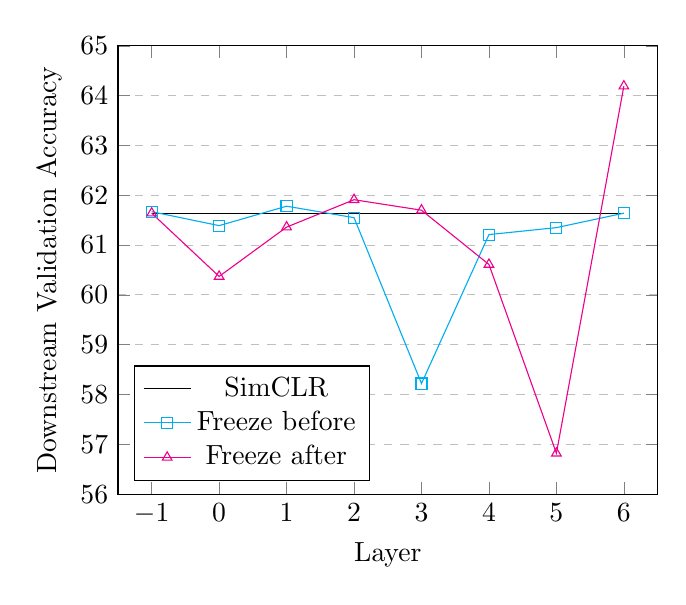
\begin{tikzpicture}
\begin{axis}[
    %title={Temperature dependence of CuSO\(_4\cdot\)5H\(_2\)O solubility},
    % width=0.8\textwidth,
    % height=0.5\textwidth,
    xlabel={Layer},
    ylabel={Downstream Validation Accuracy},
    xmin=-1.5, xmax=6.5,
    ymin=56, ymax=65,
    xtick={-1,0,1,2,3,4,5,6,7}, %,11,12,13},
    ytick={56, 57, 58, 59, 60, 61, 62, 63, 64, 65},
    %ytick={0,0.2,0.4,0.6,0.8,1.0}, %,0.6,0.7,0.8,0.9,1.0},
    legend pos=south west,
    ymajorgrids=true,
    grid style=dashed,
]
% \addplot[
%     color=black,
%     mark=diamond,
%     ]
%     coordinates {
%     % (300,62.14999771118164)(600,63.15999984741211)(900,62.91999816894531)(1200,62.29999923706055)(1500,61.93000030517578)
%     (0,61.64)
%     (1,61.64)
%     (2,61.64)
%     (3,61.64)
%     (4,61.64)
%     (5,61.64)
%     (6,61.64)
%     (7,61.64)
%     };
%     \addlegendentry{SimCLR}
\addplot[
    %dotted,
    %dashed,
    mark options={solid},
    color=black,
    %mark=diamond,
    ]
    coordinates {
    % (300,62.14999771118164)(600,63.15999984741211)(900,62.91999816894531)(1200,62.29999923706055)(1500,61.93000030517578)
    (-1,61.64)
    (0,61.64)
    (1,61.64)
    (2,61.64)
    (3,61.64)
    (4,61.64)
    (5,61.64)
    (6,61.64)
    % below is conitnue simclr
    % (-1,61.91999816894531)
    % (0,61.91999816894531)
    % (1,61.91999816894531)
    % (2,61.91999816894531)
    % (3,61.91999816894531)
    % (4,61.91999816894531)
    % (5,61.91999816894531)
    % (6,61.91999816894531)
    };
    \addlegendentry{SimCLR}
\addplot[
    color=cyan,
    mark=square,
    ]
    coordinates {
    (-1, 61.66999816894531)
    (0, 61.38999938964844)
    (1, 61.779998779296875)
    (2, 61.54999923706055)
    (3, 58.21999740600586)
    (4, 61.209999084472656)
    (5, 61.349998474121094)
    (6, 61.64)
    };
    \addlegendentry{Freeze before}
% \addplot[
%     dashed,
%     mark options={solid},
%     color=blue,
%     mark=square,
%     ]
%     coordinates {
%     (0, 61.66999816894531)
%     (1, 61.47999954223633)
%     (2, 61.939998626708984)
%     (3, 62.0099983215332)
%     (4, 62.93000030517578)
%     (5, 64.0999984741211)
%     (6, 60.09000015258789)
%     (7, 64.18999481201172)
%     };
%     \addlegendentry{Stop*}
\addplot[
    color=magenta,
    mark=triangle,
    ]
    coordinates {
    (-1, 61.64)
    (0, 60.369998931884766)
    (1, 61.3599967956543)
    (2, 61.90999984741211)
    (3, 61.69999694824219)
    (4, 60.6099967956543)
    (5, 56.81999969482422)
    (6, 64.18999481201172) % 61.91999816894531)
    };
    \addlegendentry{Freeze after}
% \addplot[
%     dashed,
%     mark options={solid},
%     color=red,
%     mark=triangle,
%     ]
%     coordinates {
%     (0, 61.66999816894531)
%     (1, 61.59000015258789)
%     (2, 61.55999755859375)
%     (3, 61.849998474121094)
%     (4, 62.21999740600586)
%     (5, 59.62999725341797)
%     (6, 58.68000030517578)
%     (7, 61.5099983215332)
%     };
%     \addlegendentry{w/o Stop*}


\end{axis}
\end{tikzpicture}
}
\vspace{-.1in}
%\caption{Continue CIFAR100-CIFAR100}
\caption{Freezing layers before and after Deep Augmentation with stop-gradient, initialized with pre-trained SimCLR model. For ``Freeze before,'' Layer -1 freezes nothing, and for ``Freeze after'' Layer 6 freezes nothing.\vspace{-.1in}}
\label{fig:CIFAR100-CIFAR100-freeze}
%\vspace{-0.5cm}
\end{figure}

\subsection{PCA Augmentation}


In Figure \ref{fig:CIFAR100-CIFAR100-stop-vs-not-pca-1-N}, results demonstrate that removing the largest principal component from a batch sample is less effective than subtracting the sixth largest (Figure \ref{fig:CIFAR10-CIFAR10-stop-vs-not-pca-6-N}).

Figure \ref{fig:PCA-image} presents the six largest principal values from the layers of a randomly initialized ResNet18 versus one trained with SimCLR on CIFAR100. Post-SimCLR training, the distribution of values becomes more uniform, and there is a notable shift in the rank of layers before and after the training process.

% In Figure \ref{fig:CIFAR100-CIFAR100-stop-vs-not-pca-1-N} we include results of subtracting the largest principal component from a sample of the batch; this under-performs compared to subtracting the sixth largest principal component.

% In Figure \ref{fig:PCA-image}, we include the six largest principal value from the layers of a random initialized ResNet18 and one trained with SimCLR on CIFAR100. After training with SimCLR, values are more equally distributed, and the rank of the layers are significantly different before and after training. 

\begin{figure}[ht]
    \centering
    % First image
    \begin{minipage}[b]{0.33\linewidth}
        \centering
        \includegraphics[width=\linewidth]{images/pca_stats_init.png}
        \caption{Random init.}
        %\label{fig:image1}
    \end{minipage}
    \hspace{0.2in} % Space between the images
    % Second image
    \begin{minipage}[b]{0.33\linewidth}
        \centering
        \includegraphics[width=\linewidth]{images/pca_stats_simclr.png}
        \caption{After SimCLR}
        %\label{fig:image2}
    \end{minipage}
\caption{The six largest principal value from the layers of a random initialized ResNet18 and one trained with SimCLR on CIFAR100.\vspace{-.1in}}
\label{fig:PCA-image}
\end{figure}

\begin{figure}[ht]
\centering
\resizebox{0.33\columnwidth}{!}{%
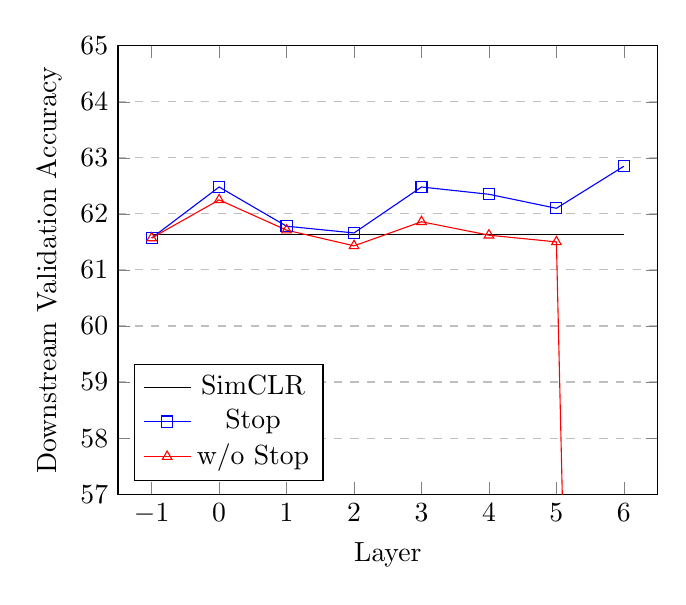
\begin{tikzpicture}
\begin{axis}[
    %title={Temperature dependence of CuSO\(_4\cdot\)5H\(_2\)O solubility},
    % width=0.8\textwidth,
    % height=0.5\textwidth,
    xlabel={Layer},
    ylabel={Downstream Validation Accuracy},
    xmin=-1.5, xmax=6.5,
    ymin=57, ymax=65,
    xtick={-1,0,1,2,3,4,5,6,7}, %,11,12,13},
    ytick={57, 58, 59, 60, 61, 62, 63, 64, 65},
    %ytick={0,0.2,0.4,0.6,0.8,1.0}, %,0.6,0.7,0.8,0.9,1.0},
    legend pos=south west,
    ymajorgrids=true,
    grid style=dashed,
]
\addplot[
    color=black,
    %mark=diamond,
    ]
    coordinates {
    % (300,62.14999771118164)(600,63.15999984741211)(900,62.91999816894531)(1200,62.29999923706055)(1500,61.93000030517578)
    (-1,61.64)
    (6,61.64)
    };
    \addlegendentry{SimCLR}
\addplot[
    %dashed,
    mark options={solid},
    color=blue,
    mark=square,
    ]
    coordinates {
    (-1, 61.57)
    (0, 62.48)
    (1, 61.78)
    (2, 61.66)
    (3, 62.48)
    (4, 62.35)
    (5, 62.1)
    (6, 62.85)
    };
    \addlegendentry{Stop}
\addplot[
    color=red,
    mark=triangle,
    ]
    coordinates {
    (-1, 61.57)
    (0, 62.25)
    (1, 61.71)
    (2, 61.43)
    (3, 61.86)
    (4, 61.62)
    (5, 61.5)
    (6, 9.85)
    };
    \addlegendentry{w/o Stop}


\end{axis}
\end{tikzpicture}
}
\vspace{-.1in}
%\caption{Continue CIFAR100-CIFAR100}
\caption{PCA: Comparing sampling 50\% of batch and subtracting the largest principal component from that sample, with and without stop-gradient.\vspace{-.1in}}
\label{fig:CIFAR100-CIFAR100-stop-vs-not-pca-1-N}
%\vspace{-0.5cm}
\end{figure}

\subsection{Supervised Learning}


For our supervised learning experiments, training was conducted for 100 epochs but otherwise using the same hyperparameters as those in the fine-tuning phase post pre-training, which lasted 28 epochs.

Figure \ref{fig:CIFAR100-CIFAR100-drop-all-vs-layer-supervised-N} presents results from supervised learning on CIFAR100, comparing the effects of uniform dropout across all layers with 50\% dropout applied to a targeted layer.

% For our supervised learning experiments, we train for a 100 epochs but otherwise with the same hyperparameters as for the fine-tuning after the pre-training step (which was fine-tuned for only 28 epochs).

% In Figure \ref{fig:CIFAR100-CIFAR100-drop-all-vs-layer-supervised-N}, we include results of supervised learning on CIFAR100, with dropout across all layers as well as 50\% dropout at targeted-layer.

Figure \ref{fig:CIFAR100-supervised-stds} presents the results of supervised training but also includes standard deviations.

\begin{figure}
\centering
\begin{subfigure}{.33\columnwidth}
\centering
\resizebox{1.0\columnwidth}{!}{%
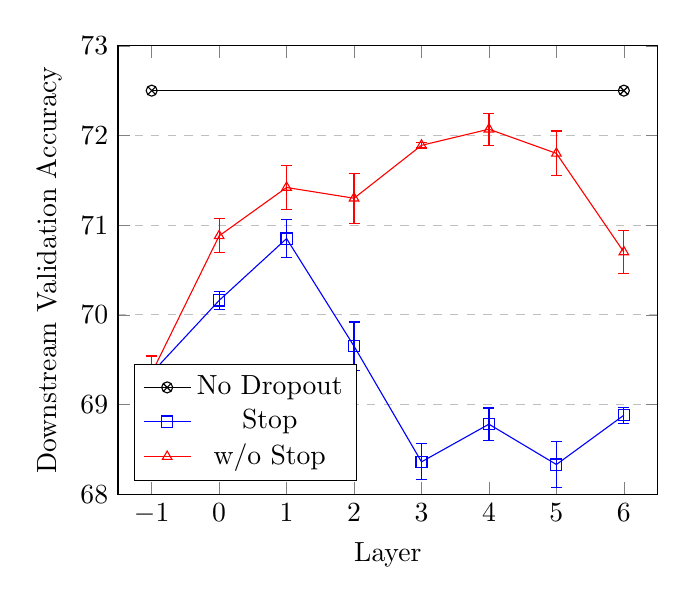
\begin{tikzpicture}
\begin{axis}[
    xlabel={Layer},
    ylabel={Downstream Validation Accuracy},
    xmin=-1.5, xmax=6.5,
    ymin=68, ymax=73,
    xtick={-1,0,1,2,3,4,5,6,7}, %,11,12,13},
    ytick={68, 69, 70, 71, 72, 73}, %57, 58, 59, 60, 61, 62, 63, 64, 65},
    legend pos=south west,
    ymajorgrids=true,
    grid style=dashed,
]
\addplot+[color=black, mark=otimes, error bars/.cd, y dir=both, y explicit, 
    ] coordinates {
    (-1, 72.5) %+- (0, 0.248797)
    (6, 72.5) %+- (0, 0.248797)
    };
    \addlegendentry{No Dropout}
\addplot+[color=blue, mark=square, error bars/.cd, y dir=both, y explicit, 
    ] coordinates {
    (-1, 69.35) +- (0,0.19)
    (0, 70.16) +- (0,0.10)
    (1, 70.85) +- (0,0.21)
    (2, 69.65) +- (0,0.27)
    (3, 68.36) +- (0,0.20)
    (4, 68.78) +- (0,0.18)
    (5, 68.33) +- (0,0.26)
    (6, 68.88) +- (0,0.09)
    };
    \addlegendentry{Stop}
% \addplot+[color=green, mark=square, error bars/.cd, y dir=both, y explicit, 
%     ] coordinates {
%     (-1, 71.82)
%     (0, 71.45)
%     (1, 71.1) 
%     (2, 69.83) 
%     (3, 68.5) 
%     (4, 68.94)
%     (5, 68.94)
%     (6, 69.02) 
%     };
%     \addlegendentry{debug}
\addplot+[color=red, mark=triangle, error bars/.cd, y dir=both, y explicit, 
    ] 
    coordinates {
    (-1, 69.35) +- (0,0.19)
    (0, 70.88) +- (0,0.19)
    (1, 71.42) +- (0,0.25)
    (2, 71.30) +- (0,0.28)
    (3, 71.89) +- (0,0.03)
    (4, 72.07) +- (0,0.18)
    (5, 71.80) +- (0,0.25)
    (6, 70.70) +- (0,0.24)
    };
    \addlegendentry{w/o Stop}
\end{axis}
\end{tikzpicture}
}
%\vspace{-.2in}
%\caption{Continue CIFAR100-CIFAR100}
\caption{Dropout}
\label{fig:CIFAR100-CIFAR100-stop-vs-not-supervised-N-stds}
\end{subfigure}%
%\hspace{0.2in}
\hspace{0.2in}
\begin{subfigure}{.33\columnwidth}
\centering
\resizebox{1.0\columnwidth}{!}{%
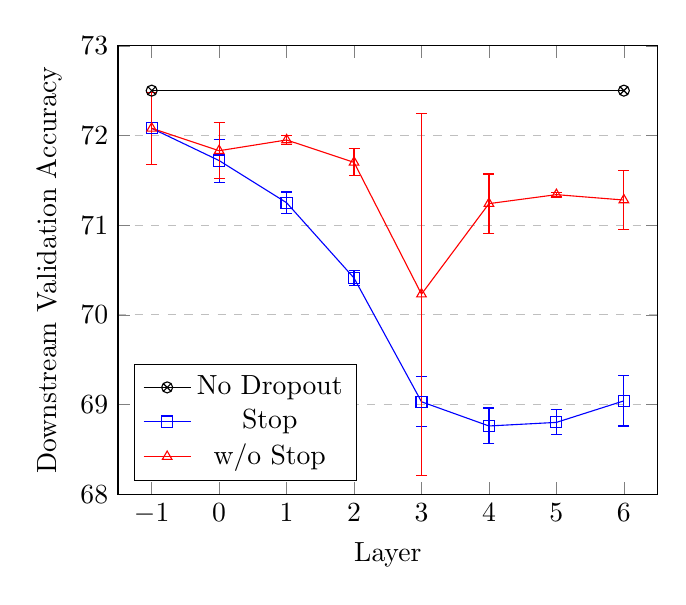
\begin{tikzpicture}
\begin{axis}[
    xlabel={Layer},
    ylabel={Downstream Validation Accuracy},
    xmin=-1.5, xmax=6.5,
    ymin=68, ymax=73,
    xtick={-1,0,1,2,3,4,5,6,7}, %,11,12,13},
    ytick={68, 69, 70, 71, 72, 73}, %57, 58, 59, 60, 61, 62, 63, 64, 65},
    legend pos=south west,
    ymajorgrids=true,
    grid style=dashed,
]
\addplot+[color=black, mark=otimes, error bars/.cd, y dir=both, y explicit, 
    ] coordinates {
    (-1, 72.5) %+- (0, 0.248797)
    (6, 72.5) %+- (0, 0.248797)
    };
    \addlegendentry{No Dropout}
% \addplot+[color=blue, mark=square, error bars/.cd, y dir=both, y explicit, 
%     ] coordinates {
%     (-1, 71.84) +- (0,0.09)
%     (0, 71.52) +- (0,0.15)
%     (1, 71.03) +- (0,0.13)
%     (2, 70.11) +- (0,0.11)
%     (3, 69.00) +- (0,0.17)
%     (4, 69.54) +- (0,0.51)
%     (5, 69.49) +- (0,0.15)
%     (6, 69.04) +- (0,0.28)
%     };
%     \addlegendentry{1 Stop}
% \addplot+[color=red, mark=triangle, error bars/.cd, y dir=both, y explicit, 
%     ] 
%     coordinates {
%     (-1, 71.84) +- (0,0.09)
%     (0, 71.93) +- (0,0.39)
%     (1, 71.91) +- (0,0.08)
%     (2, 71.73) +- (0,0.07)
%     (3, 71.94) +- (0,0.20)
%     (4, 71.63) +- (0,0.34)
%     (5, 71.52) +- (0,0.09)
%     (6, 71.70) +- (0,0.13)
%     };
%     \addlegendentry{1 w/o Stop}
\addplot+[color=blue, mark=square, error bars/.cd, y dir=both, y explicit, 
    ] coordinates {
    (-1, 72.08) +- (0,0.40)
    (0, 71.72) +- (0,0.24)
    (1, 71.25) +- (0,0.12)
    (2, 70.41) +- (0,0.08)
    (3, 69.03) +- (0,0.28)
    (4, 68.76) +- (0,0.20)
    (5, 68.80) +- (0,0.14)
    (6, 69.04) +- (0,0.28)
    };
    \addlegendentry{Stop}
\addplot+[color=red, mark=triangle, error bars/.cd, y dir=both, y explicit, 
    ] 
    coordinates {
    (-1, 72.08) +- (0,0.40)
    (0, 71.83) +- (0,0.31)
    (1, 71.95) +- (0,0.05)
    (2, 71.70) +- (0,0.15)
    (3, 70.23) +- (0,2.02)
    (4, 71.24) +- (0,0.33)
    (5, 71.34) +- (0,0.02)
    (6, 71.28) +- (0,0.33)
    };
    \addlegendentry{w/o Stop}
\end{axis}
\end{tikzpicture}
}
\vspace{-.2in}
%\caption{Continue CIFAR100-CIFAR100}
\caption{PCA}
\label{fig:CIFAR100-CIFAR100-stop-vs-not-supervised-pca6-stds}
%\vspace{-0.5cm}
\end{subfigure}
\caption{Supervised only. Deep Augmentation with (a) dropout or (b) PCA, with and without stop-gradient. *: initialized with pre-trained SimCLR model. ``Stop'' is short for stop-gradient. \vspace{-.1in}}
%\caption{Supervised only. Comparing sampling 50\% of batch and (a) applying 50\% dropout rate to or (b) removing the 6-th largest principal component from that sample, with and without stop-gradient. ``Stop'' is short for stop-gradient. No data augmentations: 59.02\%.}
%\vspace{-.1in}
\label{fig:CIFAR100-supervised-stds}
\end{figure}



%%%%%%



\begin{figure}[ht]
\centering
\resizebox{0.33\columnwidth}{!}{%
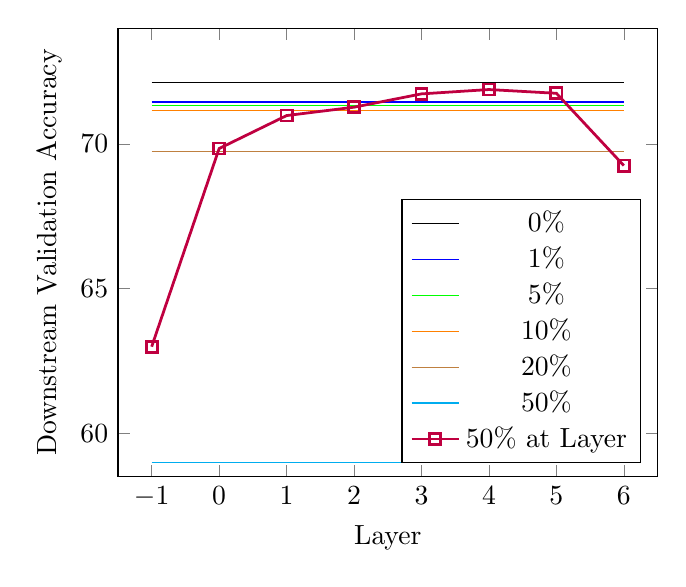
\begin{tikzpicture}
\begin{axis}[
    %title={Temperature dependence of CuSO\(_4\cdot\)5H\(_2\)O solubility},
    % width=0.8\textwidth,
    % height=0.5\textwidth,
    xlabel={Layer},
    ylabel={Downstream Validation Accuracy},
    xmin=-1.5, xmax=6.5,
    ymin=58.5, ymax=74,
    xtick={-1,0,1,2,3,4,5,6,7}, %,11,12,13},
    %ytick={51,52,53,54,55,56,57,58,59,60,61,62,63,64,65},
    ytick={50, 55, 60, 65, 70}, % ,52,53,54,55,56,57,58,59,60,61,62,63,64,65},
    %ytick={0,0.2,0.4,0.6,0.8,1.0}, %,0.6,0.7,0.8,0.9,1.0},
    legend pos=south east,
    %ymajorgrids=true,
    %grid style=dashed,
]
\addplot[
    %dashed,
    mark options={solid},
    color=black,
    %mark=diamond,
    ]
    coordinates {
    % (300,62.14999771118164)(600,63.15999984741211)(900,62.91999816894531)(1200,62.29999923706055)(1500,61.93000030517578)
    (-1,72.11)
    (6,72.11)
    };
    \addlegendentry{0\%}
\addplot[
    %dashed,
    mark options={solid},
    color=blue,
    %mark=pentagon,
    ]
    coordinates {
    (-1, 71.45)
    (6, 71.45)
    };
    \addlegendentry{1\%}
\addplot[
    %dashed,
    mark options={solid},
    color=green,
    %mark=triangle,
    ]
    coordinates {
    (-1, 71.32)
    (6, 71.32)
    };
    \addlegendentry{5\%}
\addplot[
    %dashed,
    mark options={solid},
    color=orange,
    %mark=o,
    ]
    coordinates {
    (-1, 71.14)
    (6, 71.14)
    };
    \addlegendentry{10\%}
\addplot[
    %dashed,
    mark options={solid},
    color=brown,
    %mark=diamond,
    ]
    coordinates {
    (-1, 69.73)
    (6, 69.73)
    };
    \addlegendentry{20\%}
\addplot[
    %dashed,
    mark options={solid},
    color=cyan,
    %mark=square,
    ]
    coordinates {
    (-1, 59)
    (6, 59)
    };
    \addlegendentry{50\%}

\addplot[
    % dashed,
    % mark options={solid},
    %very thick,
    line width=1pt,
    color=purple,
    mark=square,
    ]
    coordinates {
    (-1, 62.99) +- (0,1.14)
    (0, 69.84) +- (0,0.30)
    (1, 70.98) +- (0,0.16)
    (2, 71.27) +- (0,0.27)
    (3, 71.73) +- (0,0.30)
    (4, 71.88) +- (0,0.36)
    (5, 71.75) +- (0,0.22)
    (6, 69.25) +- (0,0.13)
    };
    \addlegendentry{50\% at Layer}


\end{axis}
\end{tikzpicture}
}
\vspace{-.1in}
%\caption{Continue CIFAR100-CIFAR100}
\caption{Supervised on CIFAR100: Comparing dropout rates at all layers versus 50\% dropout rate targeted at a specific layer.\vspace{-.1in}}
\label{fig:CIFAR100-CIFAR100-drop-all-vs-layer-supervised-N}
%\vspace{-0.5cm}
\end{figure}

\subsection{Domain Transfer: CIFAR100 to CIFAR10}
%\subsection{CIFAR100 to CIFAR10 domain transfer}

We perform basic domain transfer experiments by taking networks pretrained on CIFAR100 and finetuning them on CIFAR10. In Figure \ref{fig:CIFAR100-CIFAR10-domain-transfer} we include results comparing SimCLR with Deep Augmentation with and without stop-gradient, across layers. We also include performance for different checkpoints across training, see Figure \ref{fig:CIFAR100-CIFAR10-stop} and Figure \ref{fig:CIFAR100-CIFAR10-train} for Deep Augmentation with and without stop gradient, respectively. Note the overfitting tendencies.

\begin{figure}[ht]
\centering
\resizebox{0.33\columnwidth}{!}{%
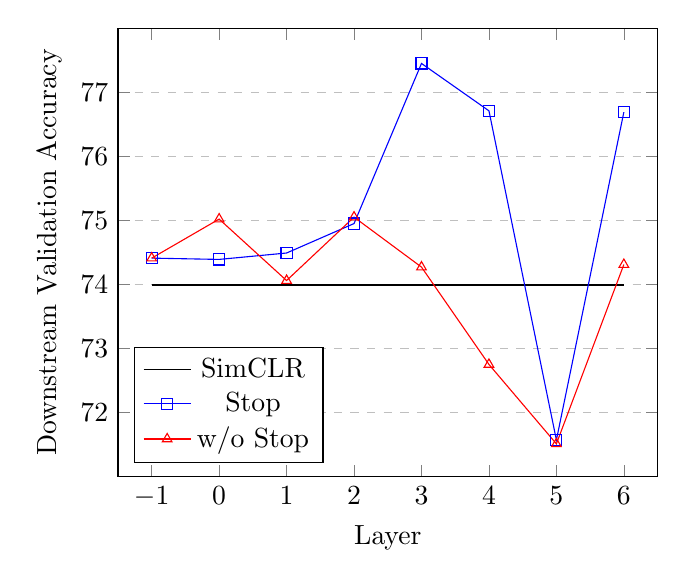
\begin{tikzpicture}
\begin{axis}[
    %title={Temperature dependence of CuSO\(_4\cdot\)5H\(_2\)O solubility},
    % width=0.8\textwidth,
    % height=0.5\textwidth,
    xlabel={Layer},
    ylabel={Downstream Validation Accuracy},
    xmin=-1.5, xmax=6.5,
    ymin=71, ymax=78,
    xtick={-1,0,1,2,3,4,5,6,7}, %,11,12,13},
    ytick={72,73,74,75,76,77},
    %ytick={0,0.2,0.4,0.6,0.8,1.0}, %,0.6,0.7,0.8,0.9,1.0},
    legend pos=south west,
    ymajorgrids=true,
    grid style=dashed,
]
\addplot[
    color=black,
    %mark=diamond,
    ]
    coordinates {
    % (300,62.14999771118164)(600,63.15999984741211)(900,62.91999816894531)(1200,62.29999923706055)(1500,61.93000030517578)
    (-1,73.98999786376953)
    (0,73.98999786376953)
    (1,73.98999786376953)
    (2,73.98999786376953)
    (3,73.98999786376953)
    (4,73.98999786376953)
    (5,73.98999786376953)
    (6,73.98999786376953)
    };
    \addlegendentry{SimCLR}
% \addplot[
%     %dotted,
%     dashed,
%     mark options={solid},
%     color=black,
%     mark=diamond,
%     ]
%     coordinates {
%     % (300,62.14999771118164)(600,63.15999984741211)(900,62.91999816894531)(1200,62.29999923706055)(1500,61.93000030517578)
%     (-1,61.91999816894531)
%     (0,61.91999816894531)
%     (1,61.91999816894531)
%     (2,61.91999816894531)
%     (3,61.91999816894531)
%     (4,61.91999816894531)
%     (5,61.91999816894531)
%     (6,61.91999816894531)
%     };
%     \addlegendentry{S}
\addplot[
    color=blue,
    mark=square,
    ]
    coordinates {
    (-1, 74.40999603271484)
    (0, 74.38999938964844)
    (1, 74.48999786376953)
    (2, 74.94999694824219)
    (3, 77.45)
    (4, 76.70999908447266)
    (5, 71.56999969482422)
    (6, 76.68999481201172)
    };
    \addlegendentry{Stop}
% \addplot[
%     dashed,
%     mark options={solid},
%     color=blue,
%     mark=square,
%     ]
%     coordinates {
%     (-1, 61.66999816894531)
%     (0, 61.47999954223633)
%     (1, 61.939998626708984)
%     (2, 62.0099983215332)
%     (3, 62.93000030517578)
%     (4, 64.0999984741211)
%     (5, 60.09000015258789)
%     (6, 64.18999481201172)
%     };
%     \addlegendentry{Stop*}
\addplot[
    color=red,
    mark=triangle,
    ]
    coordinates {
    (-1, 74.40999603271484)
    (0, 75.0199966430664)
    (1, 74.05999755859375)
    (2, 75.04999542236328)
    (3, 74.2699966430664)
    (4, 72.75)
    (5, 71.50999450683594)
    (6, 74.30999755859375)
    };
    \addlegendentry{w/o Stop}
% \addplot[
%     dashed,
%     mark options={solid},
%     color=red,
%     mark=triangle,
%     ]
%     coordinates {
%     (0, 61.66999816894531)
%     (1, 61.59000015258789)
%     (2, 61.55999755859375)
%     (3, 61.849998474121094)
%     (4, 62.21999740600586)
%     (5, 59.62999725341797)
%     (6, 58.68000030517578)
%     (7, 61.5099983215332)
%     };
%     \addlegendentry{w/o Stop*}


\end{axis}
\end{tikzpicture}
}
%\vspace{-.1in}
%\caption{Continue CIFAR100-CIFAR100}
\caption{Finetuning on CIFAR10 of networks pre-trained on CIFAR100. Comparing SimCLR with Deep Augmentation with and without stop-gradient. Stop: short for stop-gradient.}
\label{fig:CIFAR100-CIFAR10-domain-transfer}
%\vspace{-0.5cm}
\end{figure}

% \begin{figure}[ht]
% \centering
% \begin{tikzpicture}
% \begin{axis}[
%     %title={Temperature dependence of CuSO\(_4\cdot\)5H\(_2\)O solubility},
%     % width=0.8\textwidth,
%     % height=0.5\textwidth,
%     xlabel={Num. Epochs},
%     ylabel={Downstream Validation Accuracy},
%     xmin=230, xmax=1540,
%     ymin=74, ymax=80,
%     xtick={200,400,600,800,1000,1200,1400}, %,11,12,13},
%     ytick={75,76,77,78,79,80},
%     %ytick={0,0.2,0.4,0.6,0.8,1.0}, %,0.6,0.7,0.8,0.9,1.0},
%     legend pos=south west,
%     ymajorgrids=true,
%     grid style=dashed,
% ]
% \addplot[
%     color=black,
%     mark=diamond,
%     ]
%     coordinates {
%     (300,77.36000061035156)(600,77.79000091552734)(900,76.87999725341797)(1200,75.47000122070312)(1500,73.98999786376953)
%     };
%     \addlegendentry{S}

% \addplot[
%     color=blue,
%     mark=square,
%     ]
%     coordinates {
%     (600,76.98999786376953)(900,76.72000122070312)(1200,75.50999450683594)(1500,74.40999603271484)
%     };
%     \addlegendentry{L-1}
    
% \addplot[
%     color=red,
%     mark=triangle,
%     ]
%     coordinates {
%     (600,77.22000122070312)(900,76.94999694824219)(1200,74.88999938964844)(1500,74.38999938964844)
%     };
%     \addlegendentry{L0}
% \addplot[
%     color=green,
%     mark=otimes,
%     ]
%     coordinates {
%     (600,77.61000061035156)(900,77.25999450683594)(1200,75.38999938964844)(1500,74.48999786376953)
%     };
%     \addlegendentry{L1}
    
% \addplot[
%     color=pink,
%     mark=square,
%     ]
%     coordinates {
%     (600,77.83000183105469)(900,76.04999542236328)(1200,75.79000091552734)(1500,74.94999694824219)
%     };
%     \addlegendentry{L2}
% \addplot[
%     color=orange,
%     mark=diamond,
%     ]
%     coordinates {
%     (600,76.37999725341797)(900,76.75)(1200,76.93000030517578)(1500,77.45)
%     };
%     \addlegendentry{L3}
% \addplot[
%     color=yellow,
%     mark=triangle,
%     ]
%     coordinates {
%     (600,78.0199966430664)(900,79.18999481201172)(1200,78.1500015258789)(1500,76.70999908447266)
%     };
%     \addlegendentry{L4}
% \addplot[
%     color=purple,
%     mark=otimes,
%     ]
%     coordinates {
%     (600,75.16999816894531)(900,74.86000061035156)(1200,73.45999908447266)(1500,71.56999969482422)
%     };
%     \addlegendentry{L5}
% \addplot[
%     color=teal,
%     mark=square,
%     ]
%     coordinates {
%     (600,76.52999877929688)(900,78.55999755859375)(1200,78.0999984741211)(1500,76.68999481201172)
%     };
%     \addlegendentry{L6}

% \end{axis}
% \end{tikzpicture}
% %\vspace{-.1in}
% \caption{SimCLR and Deep Augmenation with stop-gradient pre-trained on CIFAR100 and finetuned on CIFAR10, for different checkpoint during training. Observe the overfitting behavior.}
% \label{fig:CIFAR100-CIFAR10-stop}
% %\vspace{-0.5cm}
% \end{figure}

% \begin{figure}[ht]
% \centering
% \begin{tikzpicture}
% \begin{axis}[
%     %title={Temperature dependence of CuSO\(_4\cdot\)5H\(_2\)O solubility},
%     % width=0.8\textwidth,
%     % height=0.5\textwidth,
%     xlabel={Num. Epochs},
%     ylabel={Downstream Validation Accuracy},
%     xmin=230, xmax=1540,
%     ymin=74, ymax=80,
%     xtick={200,400,600,800,1000,1200,1400}, %,11,12,13},
%     ytick={75,76,77,78,79,80},
%     %ytick={0,0.2,0.4,0.6,0.8,1.0}, %,0.6,0.7,0.8,0.9,1.0},
%     legend pos=south west,
%     ymajorgrids=true,
%     grid style=dashed,
% ]
% \addplot[
%     color=black,
%     mark=diamond,
%     ]
%     coordinates {
%     (300,77.36000061035156)(600,77.79000091552734)(900,76.87999725341797)(1200,75.47000122070312)(1500,73.98999786376953)
%     };
%     \addlegendentry{S}
% \addplot[
%     color=blue,
%     mark=square,
%     ]
%     coordinates {
%     (600,76.98999786376953)(900,76.72000122070312)(1200,75.50999450683594)(1500,74.40999603271484)
%     };
%     \addlegendentry{L-1}
% \addplot[
%     color=red,
%     mark=triangle,
%     ]
%     coordinates {
%     (600,77.88999938964844)(900,77.16999816894531)(1200,76.0199966430664)(1500,75.0199966430664)
%     };
%     \addlegendentry{L0}
% \addplot[
%     color=green,
%     mark=otimes,
%     ]
%     coordinates {
%     (600,77.9000015258789)(900,76.87999725341797)(1200,75.62999725341797)(1500,74.05999755859375)
%     };
%     \addlegendentry{L1}
    
% \addplot[
%     color=pink,
%     mark=square,
%     ]
%     coordinates {
%     (600,77.72000122070312)(900,77.2699966430664)(1200,75.72000122070312)(1500,75.04999542236328)
%     };
%     \addlegendentry{L2}
% \addplot[
%     color=orange,
%     mark=diamond,
%     ]
%     coordinates {
%     (600,77.83000183105469)(900,76.44999694824219)(1200,76.15999603271484)(1500,74.2699966430664)
%     };
%     \addlegendentry{L3}
% \addplot[
%     color=yellow,
%     mark=triangle,
%     ]
%     coordinates {
%     (600,75.0999984741211)(900,74.9000015258789)(1200,74.38999938964844)(1500,72.75)
%     };
%     \addlegendentry{L4}
% \addplot[
%     color=purple,
%     mark=otimes,
%     ]
%     coordinates {
%     (600,74.6500015258789)(900,73.94999694824219)(1200,72.54999542236328)(1500,71.50999450683594)
%     };
    
%     \addlegendentry{L5}
% \addplot[
%     color=teal,
%     mark=square,
%     ]
%     coordinates {
%     (600,78.22999572753906)(900,77.80999755859375)(1200,76.73999786376953)(1500,74.30999755859375)
%     };
%     \addlegendentry{L6}

% \end{axis}
% \end{tikzpicture}
% %\vspace{-.1in}
% \caption{SimCLR and Deep Augmenation without stop-gradient pre-trained on CIFAR100 and finetuned on CIFAR10, for different checkpoint during training. Observe the overfitting behavior.}
% \label{fig:CIFAR100-CIFAR10-train}
% %\vspace{-0.5cm}
% \end{figure}


\begin{figure}
\centering
\begin{subfigure}{.33\columnwidth}
\resizebox{\columnwidth}{!}{%
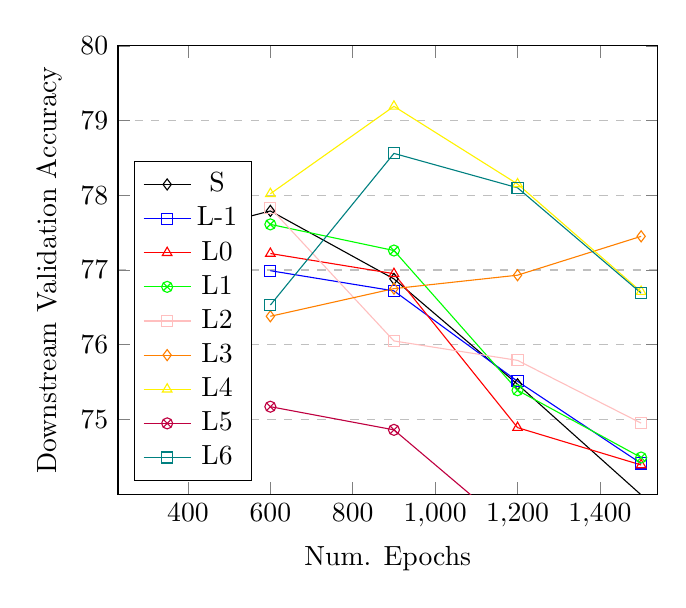
\begin{tikzpicture}
\begin{axis}[
    %title={Temperature dependence of CuSO\(_4\cdot\)5H\(_2\)O solubility},
    % width=0.8\textwidth,
    % height=0.5\textwidth,
    xlabel={Num. Epochs},
    ylabel={Downstream Validation Accuracy},
    xmin=230, xmax=1540,
    ymin=74, ymax=80,
    xtick={200,400,600,800,1000,1200,1400}, %,11,12,13},
    ytick={75,76,77,78,79,80},
    %ytick={0,0.2,0.4,0.6,0.8,1.0}, %,0.6,0.7,0.8,0.9,1.0},
    legend pos=south west,
    ymajorgrids=true,
    grid style=dashed,
]
\addplot[
    color=black,
    mark=diamond,
    ]
    coordinates {
    (300,77.36000061035156)(600,77.79000091552734)(900,76.87999725341797)(1200,75.47000122070312)(1500,73.98999786376953)
    };
    \addlegendentry{S}

\addplot[
    color=blue,
    mark=square,
    ]
    coordinates {
    (600,76.98999786376953)(900,76.72000122070312)(1200,75.50999450683594)(1500,74.40999603271484)
    };
    \addlegendentry{L-1}
    
\addplot[
    color=red,
    mark=triangle,
    ]
    coordinates {
    (600,77.22000122070312)(900,76.94999694824219)(1200,74.88999938964844)(1500,74.38999938964844)
    };
    \addlegendentry{L0}
\addplot[
    color=green,
    mark=otimes,
    ]
    coordinates {
    (600,77.61000061035156)(900,77.25999450683594)(1200,75.38999938964844)(1500,74.48999786376953)
    };
    \addlegendentry{L1}
    
\addplot[
    color=pink,
    mark=square,
    ]
    coordinates {
    (600,77.83000183105469)(900,76.04999542236328)(1200,75.79000091552734)(1500,74.94999694824219)
    };
    \addlegendentry{L2}
\addplot[
    color=orange,
    mark=diamond,
    ]
    coordinates {
    (600,76.37999725341797)(900,76.75)(1200,76.93000030517578)(1500,77.45)
    };
    \addlegendentry{L3}
\addplot[
    color=yellow,
    mark=triangle,
    ]
    coordinates {
    (600,78.0199966430664)(900,79.18999481201172)(1200,78.1500015258789)(1500,76.70999908447266)
    };
    \addlegendentry{L4}
\addplot[
    color=purple,
    mark=otimes,
    ]
    coordinates {
    (600,75.16999816894531)(900,74.86000061035156)(1200,73.45999908447266)(1500,71.56999969482422)
    };
    \addlegendentry{L5}
\addplot[
    color=teal,
    mark=square,
    ]
    coordinates {
    (600,76.52999877929688)(900,78.55999755859375)(1200,78.0999984741211)(1500,76.68999481201172)
    };
    \addlegendentry{L6}
    
\end{axis}
\end{tikzpicture}
%\vspace{-.1in}

}
%\vspace{-.1in}
\caption{With stop-gradient.}
\label{fig:CIFAR100-CIFAR10-stop}
\end{subfigure}%
\hspace{0.2in}
\begin{subfigure}{.33\columnwidth}
\centering
\resizebox{\columnwidth}{!}{%
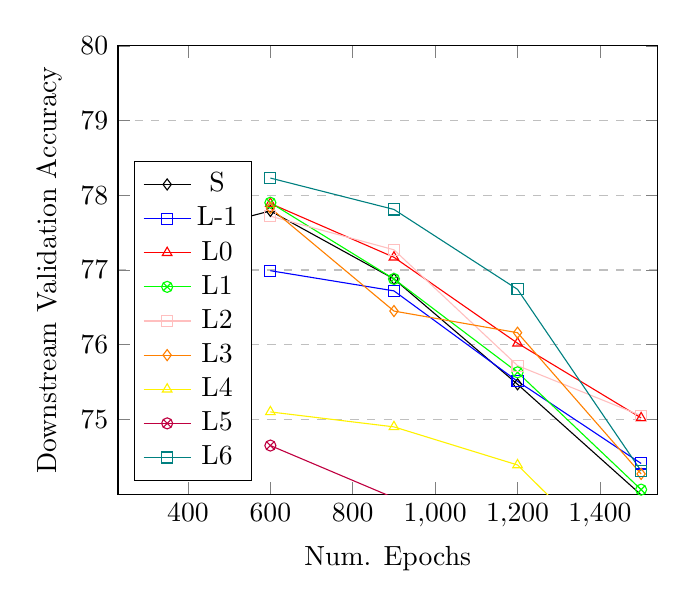
\begin{tikzpicture}
\begin{axis}[
    %title={Temperature dependence of CuSO\(_4\cdot\)5H\(_2\)O solubility},
    % width=0.8\textwidth,
    % height=0.5\textwidth,
    xlabel={Num. Epochs},
    ylabel={Downstream Validation Accuracy},
    xmin=230, xmax=1540,
    ymin=74, ymax=80,
    xtick={200,400,600,800,1000,1200,1400}, %,11,12,13},
    ytick={75,76,77,78,79,80},
    %ytick={0,0.2,0.4,0.6,0.8,1.0}, %,0.6,0.7,0.8,0.9,1.0},
    legend pos=south west,
    ymajorgrids=true,
    grid style=dashed,
]
\addplot[
    color=black,
    mark=diamond,
    ]
    coordinates {
    (300,77.36000061035156)(600,77.79000091552734)(900,76.87999725341797)(1200,75.47000122070312)(1500,73.98999786376953)
    };
    \addlegendentry{S}
\addplot[
    color=blue,
    mark=square,
    ]
    coordinates {
    (600,76.98999786376953)(900,76.72000122070312)(1200,75.50999450683594)(1500,74.40999603271484)
    };
    \addlegendentry{L-1}
\addplot[
    color=red,
    mark=triangle,
    ]
    coordinates {
    (600,77.88999938964844)(900,77.16999816894531)(1200,76.0199966430664)(1500,75.0199966430664)
    };
    \addlegendentry{L0}
\addplot[
    color=green,
    mark=otimes,
    ]
    coordinates {
    (600,77.9000015258789)(900,76.87999725341797)(1200,75.62999725341797)(1500,74.05999755859375)
    };
    \addlegendentry{L1}
    
\addplot[
    color=pink,
    mark=square,
    ]
    coordinates {
    (600,77.72000122070312)(900,77.2699966430664)(1200,75.72000122070312)(1500,75.04999542236328)
    };
    \addlegendentry{L2}
\addplot[
    color=orange,
    mark=diamond,
    ]
    coordinates {
    (600,77.83000183105469)(900,76.44999694824219)(1200,76.15999603271484)(1500,74.2699966430664)
    };
    \addlegendentry{L3}
\addplot[
    color=yellow,
    mark=triangle,
    ]
    coordinates {
    (600,75.0999984741211)(900,74.9000015258789)(1200,74.38999938964844)(1500,72.75)
    };
    \addlegendentry{L4}
\addplot[
    color=purple,
    mark=otimes,
    ]
    coordinates {
    (600,74.6500015258789)(900,73.94999694824219)(1200,72.54999542236328)(1500,71.50999450683594)
    };
    
    \addlegendentry{L5}
\addplot[
    color=teal,
    mark=square,
    ]
    coordinates {
    (600,78.22999572753906)(900,77.80999755859375)(1200,76.73999786376953)(1500,74.30999755859375)
    };
    \addlegendentry{L6}

\end{axis}
\end{tikzpicture}


}
\caption{Without stop-gradient}
\label{fig:CIFAR100-CIFAR10-train}
\end{subfigure}
\caption{SimCLR and Deep Augmenation with and without stop-gradient pre-trained on CIFAR100 and finetuned on CIFAR10, for different checkpoints during training. Observe the overfitting behavior.}
\label{fig:CIFAR100-CIFAR10}
\end{figure}

\subsection{Different dropout rates}

In Figure \ref{fig:CIFAR100-CIFAR100-stop-vs-not-rates-N}, we tune over dropout rates 0.5, 0.25, and 0.125 and find that 0.125 at Layer 4 performs the best.

\begin{figure}[ht]
\centering
\resizebox{0.33\columnwidth}{!}{%
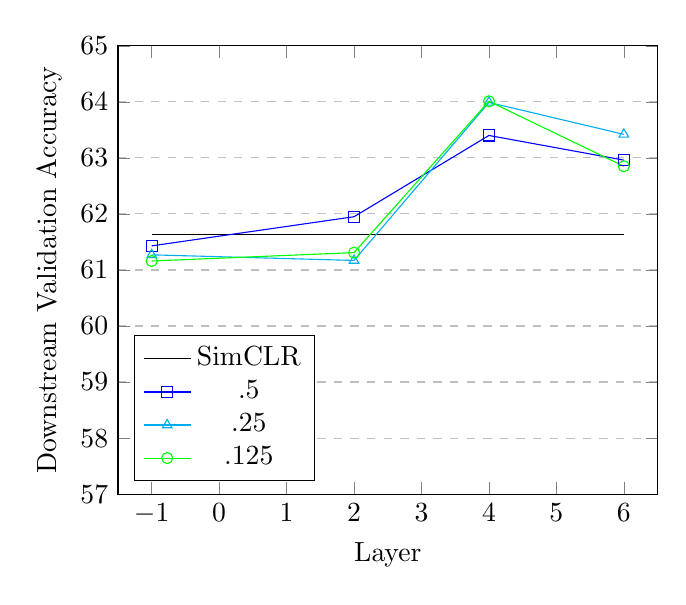
\begin{tikzpicture}
\begin{axis}[
    %title={Temperature dependence of CuSO\(_4\cdot\)5H\(_2\)O solubility},
    % width=0.8\textwidth,
    % height=0.5\textwidth,
    xlabel={Layer},
    ylabel={Downstream Validation Accuracy},
    xmin=-1.5, xmax=6.5,
    ymin=57, ymax=65,
    xtick={-1,0,1,2,3,4,5,6,7}, %,11,12,13},
    ytick={57, 58, 59, 60, 61, 62, 63, 64, 65},
    %ytick={0,0.2,0.4,0.6,0.8,1.0}, %,0.6,0.7,0.8,0.9,1.0},
    legend pos=south west,
    ymajorgrids=true,
    grid style=dashed,
]
\addplot[
    color=black,
    %mark=diamond,
    ]
    coordinates {
    % (300,62.14999771118164)(600,63.15999984741211)(900,62.91999816894531)(1200,62.29999923706055)(1500,61.93000030517578)
    (-1,61.64)
    (0,61.64)
    (1,61.64)
    (2,61.64)
    (3,61.64)
    (4,61.64)
    (5,61.64)
    (6,61.64)
    };
    \addlegendentry{SimCLR}
% \addplot[
%     %dotted,
%     dashed,
%     mark options={solid},
%     color=black,
%     %mark=diamond,
%     ]
%     coordinates {
%     % (300,62.14999771118164)(600,63.15999984741211)(900,62.91999816894531)(1200,62.29999923706055)(1500,61.93000030517578)
%     (-1,61.91999816894531)
%     (0,61.91999816894531)
%     (1,61.91999816894531)
%     (2,61.91999816894531)
%     (3,61.91999816894531)
%     (4,61.91999816894531)
%     (5,61.91999816894531)
%     (6,61.91999816894531)
%     };
%     \addlegendentry{SimCLR*}
\addplot[
    color=blue,
    mark=square,
    ]
    coordinates {
    (-1, 61.43000030517578)
    % (0, 61.269996643066406) 
    % (1, 61.38999938964844)
    (2, 61.94999694824219)
    % (3, 62.43000030517578)
    (4, 63.39999771118164)
    % (5, 58.59000015258789)
    (6, 62.959999084472656)
    };
    \addlegendentry{.5}
\addplot[
    mark options={solid},
    color=cyan,
    mark=triangle,
    ]
    coordinates {
    (-1, 61.27)
    (2, 61.17)
    (4, 63.99)
    (6, 63.42)
    };
    \addlegendentry{.25}

\addplot[
    mark options={solid},
    color=green,
    mark=o,
    ]
    coordinates {
    (-1, 61.16)
    (2, 61.31)
    (4, 64.01)
    (6, 62.85)
    };
    \addlegendentry{.125}
% \addplot[
%     mark options={solid},
%     color=lime,
%     mark=diamond,
%     ]
%     coordinates {
%     (-1, 61.77)
%     (2, 61.55)
%     (4, 63.83)
%     (6, 63.52)
%     };
%     \addlegendentry{**}

    
%\addplot[
%     color=red,
%     mark=triangle,
%     ]
%     coordinates {
%     (-1, 61.43000030517578)
%     (0, 62.029998779296875)
%     (1, 62.13999938964844)
%     (2, 61.769996643066406)
%     (3, 61.07999801635742)
%     (4, 59.519996643066406)
%     (5, 57.16999816894531)
%     (6, 61.73999786376953)
%     };
%     \addlegendentry{w/o Stop}
% \addplot[
%     dashed,
%     mark options={solid},
%     color=red,
%     mark=triangle,
%     ]
%     coordinates {
%     (-1, 61.66999816894531)
%     (0, 61.59000015258789)
%     (1, 61.55999755859375)
%     (2, 61.849998474121094)
%     (3, 62.21999740600586)
%     (4, 59.62999725341797)
%     (5, 58.68000030517578)
%     (6, 61.5099983215332)
%     };
%     \addlegendentry{w/o Stop*}


\end{axis}
\end{tikzpicture}
}
\vspace{-.2in}
%\caption{Continue CIFAR100-CIFAR100}
\caption{CIFAR100: Comparing sampling 50\% of batch and applying dropout to that sample, with and without stop-gradient, for different dropout rates. ``Stop'' is short for stop-gradient.\vspace{-.1in}}
\label{fig:CIFAR100-CIFAR100-stop-vs-not-rates-N}
%\vspace{-0.5cm}
\end{figure}


\subsection{CIFAR10}

We include results on most of the experiments that were run on CIFAR100, also on CIFAR10. In general, results show the same trends as for CIFAR100. In Figure \ref{fig:CIFAR10-CIFAR10-drop-all-vs-layer}, we include results comparing dropout rates across all layers to 50\% dropout at single layers. Again, we see targeted dropout at some layers showing much better performance than dropout across all layers. 

In Figure \ref{fig:CIFAR10-compare} we include results of sampling 50\% of batch and performing 50\% dropout with and without stop-gradient, called ``Stop'' and ``w/o Stop'' respectively. We also include a benchmark of SimCLR. Here ``*'' refers to the networks being initialized with a pre-trained SimCLR model. Again, we see Layer 4 (with stop-gradient) and Layer 6 (with and without stop-gradient) stand out. It is also interesting to note that when initializing with a pre-trained SimCLR model, performance differs significantly more for Deep Augmentation with stop-gradient than without.

In Figures \ref{fig:CIFAR10-CIFAR10-stop-vs-not-pca-1-N} and \ref{fig:CIFAR10-CIFAR10-stop-vs-not-pca-6-N}, we subtract the largest and sixth largest principal component from half the samples of the batch. 

\begin{figure}[ht]
\centering
\resizebox{0.33\columnwidth}{!}{%
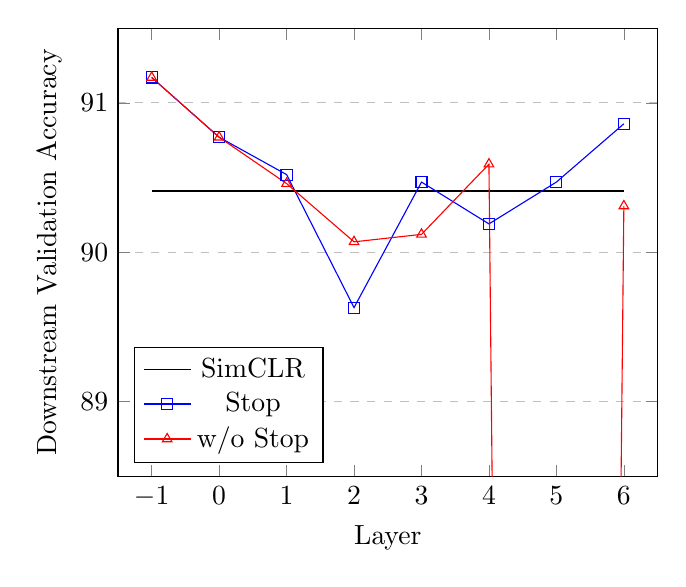
\begin{tikzpicture}
\begin{axis}[
    %title={Temperature dependence of CuSO\(_4\cdot\)5H\(_2\)O solubility},
    % width=0.8\textwidth,
    % height=0.5\textwidth,
    xlabel={Layer},
    ylabel={Downstream Validation Accuracy},
    xmin=-1.5, xmax=6.5,
    ymin=88.5, ymax=91.5,
    xtick={-1,0,1,2,3,4,5,6,7}, %,11,12,13},
    ytick={89,90,91},
    %ytick={0,0.2,0.4,0.6,0.8,1.0}, %,0.6,0.7,0.8,0.9,1.0},
    legend pos=south west,
    ymajorgrids=true,
    grid style=dashed,
]
\addplot[
    color=black,
    %mark=diamond,
    ]
    coordinates {
    % (300,62.14999771118164)(600,63.15999984741211)(900,62.91999816894531)(1200,62.29999923706055)(1500,61.93000030517578)
    (-1,90.40999603271484)
    (6,90.40999603271484)
    };
    \addlegendentry{SimCLR}
\addplot[
    %dashed,
    mark options={solid},
    color=blue,
    mark=square,
    ]
    coordinates {
    (-1, 91.17)
    (0, 90.77)
    (1, 90.52)
    (2, 89.63)
    (3, 90.47)
    (4, 90.19)
    (5, 90.47)
    (6, 90.86)
    };
    \addlegendentry{Stop}
\addplot[
    color=red,
    mark=triangle,
    ]
    coordinates {
    (-1, 91.17)
    (0, 90.77)
    (1, 90.46)
    (2, 90.07)
    (3, 90.12)
    (4, 90.59)
    (5, 46.04)
    (6, 90.31)
    };
    \addlegendentry{w/o Stop}


\end{axis}
\end{tikzpicture}
}
\vspace{-.2in}
%\caption{Continuear100-CIFAR100}
\caption{PCA CIFAR10: Comparing sampling 50\% of batch and subtracting the largest principal component from that sample, with and without stop-gradient.\vspace{-.1in}}
\label{fig:CIFAR10-CIFAR10-stop-vs-not-pca-1-N}
%\vspace{-0.5cm}
\end{figure}


\begin{figure}[ht]
\centering
\resizebox{0.33\columnwidth}{!}{%
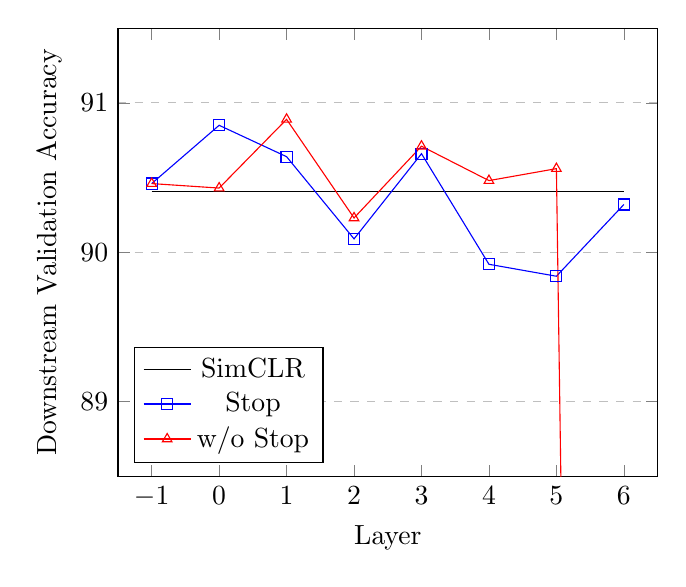
\begin{tikzpicture}
\begin{axis}[
    %title={Temperature dependence of CuSO\(_4\cdot\)5H\(_2\)O solubility},
    % width=0.8\textwidth,
    % height=0.5\textwidth,
    xlabel={Layer},
    ylabel={Downstream Validation Accuracy},
    xmin=-1.5, xmax=6.5,
    ymin=88.5, ymax=91.5,
    xtick={-1,0,1,2,3,4,5,6,7}, %,11,12,13},
    ytick={89,90,91},
    %ytick={0,0.2,0.4,0.6,0.8,1.0}, %,0.6,0.7,0.8,0.9,1.0},
    legend pos=south west,
    ymajorgrids=true,
    grid style=dashed,
]
\addplot[
    color=black,
    %mark=diamond,
    ]
    coordinates {
    % (300,62.14999771118164)(600,63.15999984741211)(900,62.91999816894531)(1200,62.29999923706055)(1500,61.93000030517578)
    (-1,90.40999603271484)
    (6,90.40999603271484)
    };
    \addlegendentry{SimCLR}
\addplot[
    %dashed,
    mark options={solid},
    color=blue,
    mark=square,
    ]
    coordinates {
    (-1, 90.46)
    (0, 90.85)
    (1, 90.64)
    (2, 90.09)
    (3, 90.66)
    (4, 89.92)
    (5, 89.84)
    (6, 90.32)
    };
    \addlegendentry{Stop}
\addplot[
    color=red,
    mark=triangle,
    ]
    coordinates {
    (-1, 90.46)
    (0, 90.43)
    (1, 90.89)
    (2, 90.23)
    (3, 90.71)
    (4, 90.48)
    (5, 90.56)
    (6, 59.32)
    };
    \addlegendentry{w/o Stop}


\end{axis}
\end{tikzpicture}
}
\vspace{-.1in}
%\caption{Continuear100-CIFAR100}
\caption{PCA CIFAR10: Comparing sampling 50\% of batch and subtracting the sixth principal component from that sample, with and without stop-gradient.}
\label{fig:CIFAR10-CIFAR10-stop-vs-not-pca-6-N}
%\vspace{-0.5cm}
\end{figure}

In Figure \ref{fig:CIFAR10-freeze}, we include results of Deep Augmentation with stop-gradient but freezing layers up to the targeted layer versus freezing after the targeted layer. Again, we see the performance change, especially Layer 3 and 4 degrading, while Layer 2 improves. 


In Figure \ref{fig:CIFAR10-CIFAR10-drop-all-vs-layer-supervised-N}, we include results of supervised learning on CIFAR10, with dropout across all layers as well as 50\% dropout at targeted-layer.

\begin{figure}[ht]
\centering
\resizebox{0.33\columnwidth}{!}{%
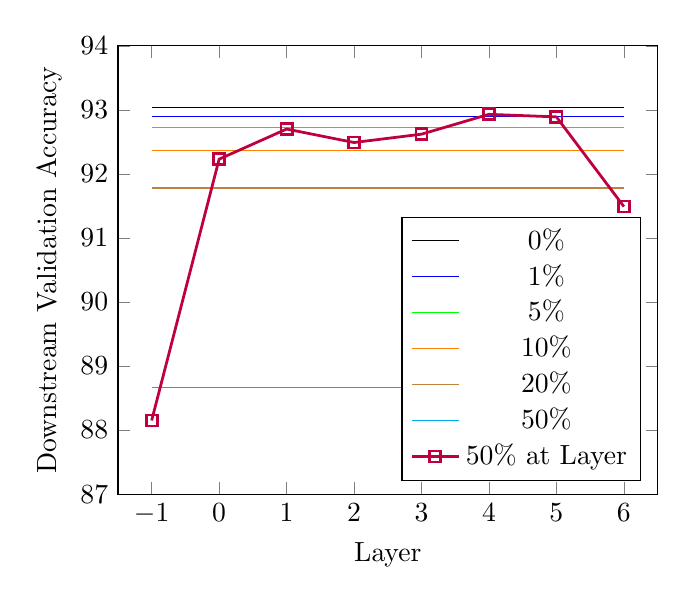
\begin{tikzpicture}
\begin{axis}[
    %title={Temperature dependence of CuSO\(_4\cdot\)5H\(_2\)O solubility},
    % width=0.8\textwidth,
    % height=0.5\textwidth,
    xlabel={Layer},
    ylabel={Downstream Validation Accuracy},
    xmin=-1.5, xmax=6.5,
    ymin=87, ymax=94,
    xtick={-1,0,1,2,3,4,5,6,7}, %,11,12,13},
    %ytick={51,52,53,54,55,56,57,58,59,60,61,62,63,64,65},
    ytick={87,88,89,90,91,92,93,94}, % ,52,53,54,55,56,57,58,59,60,61,62,63,64,65},
    %ytick={0,0.2,0.4,0.6,0.8,1.0}, %,0.6,0.7,0.8,0.9,1.0},
    legend pos=south east,
    %ymajorgrids=true,
    %grid style=dashed,
]
\addplot[
    %dashed,
    mark options={solid},
    color=black,
    %mark=diamond,
    ]
    coordinates {
    (-1, 93.03)
    (6, 93.03)
    };
    \addlegendentry{0\%}
\addplot[
    %dashed,
    mark options={solid},
    color=blue,
    %mark=pentagon,
    ]
    coordinates {
    (-1, 92.9)
    (6, 92.9)
    };
    \addlegendentry{1\%}
\addplot[
    %dashed,
    mark options={solid},
    color=green,
    %mark=triangle,
    ]
    coordinates {
    (-1, 92.72)
    (6, 92.72)
    };
    \addlegendentry{5\%}
\addplot[
    %dashed,
    mark options={solid},
    color=orange,
    %mark=o,
    ]
    coordinates {
    (-1, 92.37)
    (6, 92.37)
    };
    \addlegendentry{10\%}
\addplot[
    %dashed,
    mark options={solid},
    color=brown,
    %mark=diamond,
    ]
    coordinates {
    (-1, 91.78)
    (6, 91.78)
    };
    \addlegendentry{20\%}
\addplot[
    %dashed,
    mark options={solid},
    color=cyan,
    %mark=square,
    ]
    coordinates {
    (-1, 88.67)
    (6, 88.67)
    };
    \addlegendentry{50\%}
\addplot[
    % dashed,
    % mark options={solid},
    %very thick,
    line width=1pt,
    color=purple,
    mark=square,
    ]
    coordinates {
    (-1, 88.15) +- (0,0.35)
    (0, 92.23) +- (0,0.10)
    (1, 92.70) +- (0,0.04)
    (2, 92.49) +- (0,0.20)
    (3, 92.62) +- (0,0.07)
    (4, 92.93) +- (0,0.12)
    (5, 92.89) +- (0,0.07)
    (6, 91.49) +- (0,0.23)
    };
    \addlegendentry{50\% at Layer}
\end{axis}
\end{tikzpicture}
}
\vspace{-.1in}
%\caption{Continue CIFAR100-CIFAR100}
\caption{Supervised on CIFAR10: Comparing dropout rates at all layers versus 50\% dropout rate targeted at a specific layer.}
\label{fig:CIFAR10-CIFAR10-drop-all-vs-layer-supervised-N}
%\vspace{-0.5cm}
\end{figure}

We perform basic domain transfer experiments by taking networks pretrained on CIFAR10 and finetuning them on CIFAR100. In Figure \ref{fig:CIFAR10-CIFAR100-domain} we include results comparing SimCLR with Deep Augmentation with and without stop-gradient, across layers. We also include performance for different checkpoints across training, see Figure \ref{fig:CIFAR10-CIFAR100-stop} and Figure \ref{fig:CIFAR10-CIFAR100-train} for Deep Augmentation with and without stop gradient, respectively. Note the overfitting tendencies.


In Figure \ref{fig:CIFAR10-compare-rates-N}, we tune over dropout rates 0.5, 0.25, and 0.125 and fine that 0.125 at Layer 4 performs the best.

\begin{figure}[ht]
\centering
\resizebox{0.33\columnwidth}{!}{%
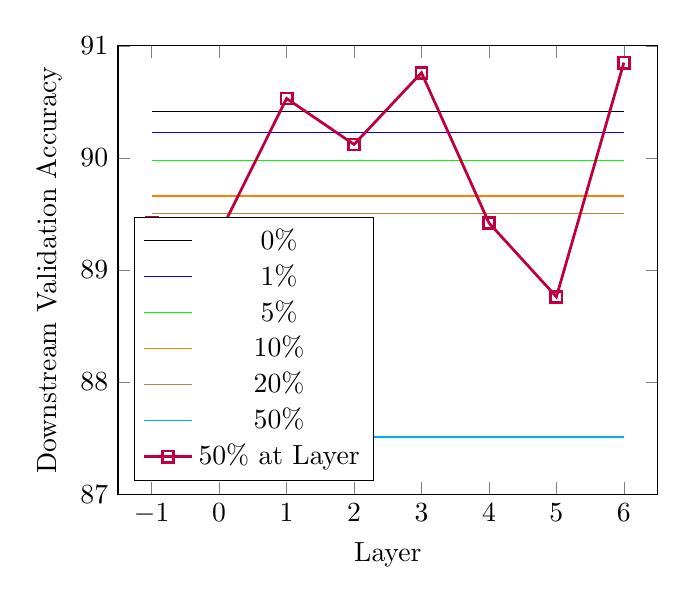
\begin{tikzpicture}
\begin{axis}[
    %title={Temperature dependence of CuSO\(_4\cdot\)5H\(_2\)O solubility},
    % width=0.8\textwidth,
    % height=0.5\textwidth,
    xlabel={Layer},
    ylabel={Downstream Validation Accuracy},
    xmin=-1.5, xmax=6.5,
    ymin=87, ymax=91,
    xtick={-1,0,1,2,3,4,5,6,7}, %,11,12,13},
    %ytick={51,52,53,54,55,56,57,58,59,60,61,62,63,64,65},
    ytick={87,88,89,90,91}, % ,52,53,54,55,56,57,58,59,60,61,62,63,64,65},
    %ytick={0,0.2,0.4,0.6,0.8,1.0}, %,0.6,0.7,0.8,0.9,1.0},
    legend pos=south west,
    %ymajorgrids=true,
    %grid style=dashed,
]
\addplot[
    %dashed,
    mark options={solid},
    color=black,
    %mark=diamond,
    ]
    coordinates {
    % (300,62.14999771118164)(600,63.15999984741211)(900,62.91999816894531)(1200,62.29999923706055)(1500,61.93000030517578)
    (-1,90.40999603271484)
    (0,90.40999603271484)
    (1,90.40999603271484)
    (2,90.40999603271484)
    (3,90.40999603271484)
    (4,90.40999603271484)
    (5,90.40999603271484)
    (6,90.40999603271484)
    };
    \addlegendentry{0\%}
\addplot[
    %dashed,
    mark options={solid},
    color=blue,
    %mark=pentagon,
    ]
    coordinates {
    (-1, 90.22999572753906)
    (0, 90.22999572753906) 
    (1, 90.22999572753906)
    (2, 90.22999572753906)
    (3, 90.22999572753906)
    (4, 90.22999572753906)
    (5, 90.22999572753906)
    (6, 90.22999572753906)
    };
    \addlegendentry{1\%}
\addplot[
    %dashed,
    mark options={solid},
    color=green,
    %mark=triangle,
    ]
    coordinates {
    (-1, 89.97999572753906)
    (0, 89.97999572753906)
    (1, 89.97999572753906)
    (2, 89.97999572753906)
    (3, 89.97999572753906)
    (4, 89.97999572753906)
    (5, 89.97999572753906)
    (6, 89.97999572753906)
    };
    \addlegendentry{5\%}
\addplot[
    %dashed,
    mark options={solid},
    color=orange,
    %mark=o,
    ]
    coordinates {
    (-1, 89.65999603271484)
    (0, 89.65999603271484)
    (1, 89.65999603271484)
    (2, 89.65999603271484)
    (3, 89.65999603271484)
    (4, 89.65999603271484)
    (5, 89.65999603271484)
    (6, 89.65999603271484)
    };
    \addlegendentry{10\%}
\addplot[
    %dashed,
    mark options={solid},
    color=brown,
    %mark=diamond,
    ]
    coordinates {
    (-1, 89.5)
    (0, 89.5)
    (1, 89.5)
    (2, 89.5)
    (3, 89.5)
    (4, 89.5)
    (5, 89.5)
    (6, 89.5)
    };
    \addlegendentry{20\%}
\addplot[
    %dashed,
    mark options={solid},
    color=cyan,
    %mark=square,
    ]
    coordinates {
    (-1, 87.50999450683594)
    (0, 87.50999450683594)
    (1, 87.50999450683594)
    (2, 87.50999450683594)
    (3, 87.50999450683594)
    (4, 87.50999450683594)
    (5, 87.50999450683594)
    (6, 87.50999450683594)
    };
    \addlegendentry{50\%}

\addplot[
    % dashed,
    % mark options={solid},
    %very thick,
    line width=1pt,
    color=purple,
    mark=square,
    ]
    coordinates {
    (-1, 89.41999816894531)
    (0, 89.31999969482422)
    (1, 90.52999877929688)
    (2, 90.1199951171875)
    (3, 90.75999450683594)
    (4, 89.41999816894531)
    (5, 88.75999450683594)
    (6, 90.8499984741211)
    % (-1, 90.3699951171875)
    % (0, 90.41999816894531)
    % (1, 90.54000091552734)
    % (2, 90.40999603271484)
    % (3, 90.40999603271484)
    % (4, 89.80999755859375)
    % (5, 89.5)
    % (6, 90.82999420166016)
    };
    \addlegendentry{50\% at Layer}


\end{axis}
\end{tikzpicture}
}
%\vspace{-.1in}
%\caption{Continue CIFAR100-CIFAR100}
\caption{CIFAR10: Comparing dropout rates at all layers versus 50\% dropout targeted at a specific layer.}
\label{fig:CIFAR10-CIFAR10-drop-all-vs-layer}
%\vspace{-0.5cm}
\end{figure}

\begin{figure}[ht]
\centering
\resizebox{0.33\columnwidth}{!}{%
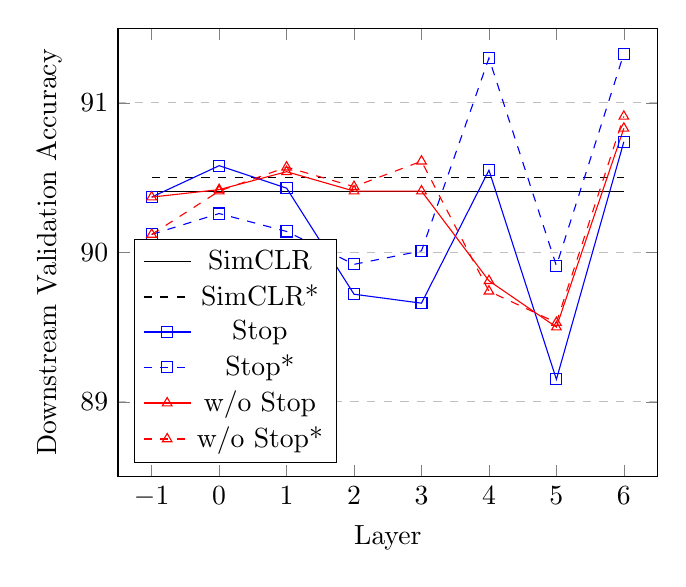
\begin{tikzpicture}
\begin{axis}[
    %title={Temperature dependence of CuSO\(_4\cdot\)5H\(_2\)O solubility},
    % width=0.8\textwidth,
    % height=0.5\textwidth,
    xlabel={Layer},
    ylabel={Downstream Validation Accuracy},
    xmin=-1.5, xmax=6.5,
    ymin=88.5, ymax=91.5,
    xtick={-1,0,1,2,3,4,5,6,7}, %,11,12,13},
    ytick={89,90,91},
    %ytick={0,0.2,0.4,0.6,0.8,1.0}, %,0.6,0.7,0.8,0.9,1.0},
    legend pos=south west,
    ymajorgrids=true,
    grid style=dashed,
]
\addplot[
    color=black,
    %mark=diamond,
    ]
    coordinates {
    % (300,62.14999771118164)(600,63.15999984741211)(900,62.91999816894531)(1200,62.29999923706055)(1500,61.93000030517578)
    (-1,90.40999603271484)
    (0,90.40999603271484)
    (1,90.40999603271484)
    (2,90.40999603271484)
    (3,90.40999603271484)
    (4,90.40999603271484)
    (5,90.40999603271484)
    (6,90.40999603271484)
    
    };
    \addlegendentry{SimCLR}
\addplot[
    %dotted,
    dashed,
    mark options={solid},
    color=black,
    %mark=diamond,
    ]
    coordinates {
    % (300,62.14999771118164)(600,63.15999984741211)(900,62.91999816894531)(1200,62.29999923706055)(1500,61.93000030517578)
    (-1,90.5)
    (0,90.5)
    (1,90.5)
    (2,90.5)
    (3,90.5)
    (4,90.5)
    (5,90.5)
    (6,90.5)
    };
    \addlegendentry{SimCLR*}
\addplot[
    color=blue,
    mark=square,
    ]
    coordinates {
    (-1, 90.3699951171875)
    (0, 90.57999420166016)
    (1, 90.43000030517578)
    (2, 89.72000122070312)
    (3, 89.65999603271484)
    (4, 90.54999542236328)
    (5, 89.1500015258789)
    (6, 90.73999786376953)
    
    % (-1,90.1199951171875)
    % (0, 90.25999450683594)
    % (1, 90.13999938964844)
    % (2, 89.91999816894531)
    % (3, 90.00999450683594)
    % (4, 91.29999542236328)
    % (5, 89.90999603271484)
    % (6, 91.32999420166016)
    };
    \addlegendentry{Stop}
\addplot[
    dashed,
    mark options={solid},
    color=blue,
    mark=square,
    ]
    coordinates {
    (-1,90.1199951171875)
    (0, 90.25999450683594)
    (1, 90.13999938964844)
    (2, 89.91999816894531)
    (3, 90.00999450683594)
    (4, 91.29999542236328)
    (5, 89.90999603271484)
    (6, 91.32999420166016)
    };
    \addlegendentry{Stop*}
\addplot[
    color=red,
    mark=triangle,
    ]
    coordinates {
    (-1, 90.3699951171875)
    (0, 90.41999816894531)
    (1, 90.54000091552734)
    (2, 90.40999603271484)
    (3, 90.40999603271484)
    (4, 89.80999755859375)
    (5, 89.5)
    (6, 90.82999420166016)
    };
    \addlegendentry{w/o Stop}
\addplot[
    dashed,
    mark options={solid},
    color=red,
    mark=triangle,
    ]
    coordinates {
    (-1, 90.1199951171875)
    (0, 90.40999603271484)
    (1, 90.56999969482422)
    (2, 90.43999481201172)
    (3, 90.61000061035156)
    (4, 89.73999786376953)
    (5, 89.52999877929688)
    (6, 90.90999603271484)
    };
    \addlegendentry{w/o Stop*}


\end{axis}
\end{tikzpicture}
}
%\vspace{-.1in}
%\caption{Continue CIFAR100-CIFAR100}
\caption{CIFAR10: Comparing SimCLR with Deep Augmentation with and without stop-gradient. *: Initialized with pre-trained SimCLR model. Stop: short for stop-gradient.}
\label{fig:CIFAR10-compare}
%\vspace{-0.5cm}
\end{figure}


\begin{figure}[ht]
\centering
\resizebox{0.33\columnwidth}{!}{%
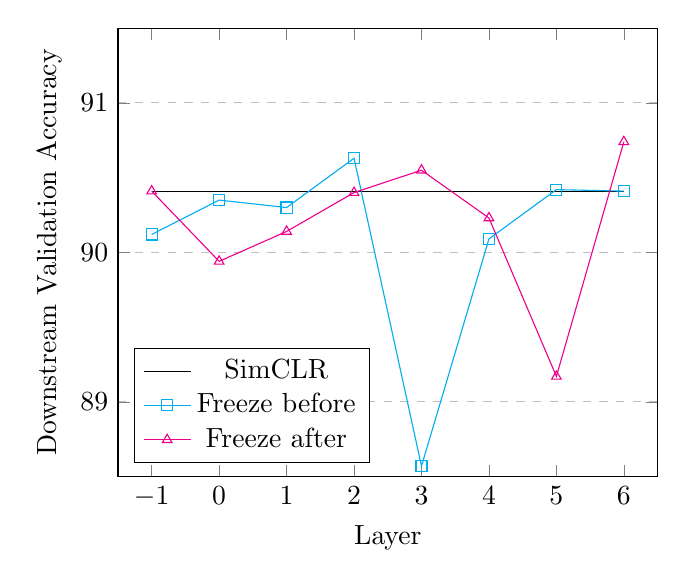
\begin{tikzpicture}
\begin{axis}[
    %title={Temperature dependence of CuSO\(_4\cdot\)5H\(_2\)O solubility},
    % width=0.8\textwidth,
    % height=0.5\textwidth,
    xlabel={Layer},
    ylabel={Downstream Validation Accuracy},
    xmin=-1.5, xmax=6.5,
    ymin=88.5, ymax=91.5,
    xtick={-1,0,1,2,3,4,5,6,7}, %,11,12,13},
    ytick={89,90,91},
    %ytick={0,0.2,0.4,0.6,0.8,1.0}, %,0.6,0.7,0.8,0.9,1.0},
    legend pos=south west,
    ymajorgrids=true,
    grid style=dashed,
]
\addplot[
    color=black,
    %mark=diamond,
    ]
    coordinates {
    % (300,62.14999771118164)(600,63.15999984741211)(900,62.91999816894531)(1200,62.29999923706055)(1500,61.93000030517578)
    (-1,90.40999603271484)
    (0,90.40999603271484)
    (1,90.40999603271484)
    (2,90.40999603271484)
    (3,90.40999603271484)
    (4,90.40999603271484)
    (5,90.40999603271484)
    (6,90.40999603271484)
    
    };
    \addlegendentry{SimCLR}
\addplot[
    color=cyan,
    mark=square,
    ]
    coordinates {
    (-1, 90.1199951171875)
    (0, 90.3499984741211)
    (1, 90.29999542236328)
    (2, 90.62999725341797)
    (3, 88.56999969482422)
    (4, 90.08999633789062)
    (5, 90.41999816894531)
    (6, 90.40999603271484)
    
    % (-1, 90.3699951171875)
    % (0, 90.41999816894531)
    % (1, 90.54000091552734)
    % (2, 90.40999603271484)
    % (3, 90.40999603271484)
    % (4, 89.80999755859375)
    % (5, 89.5)
    % (6, 90.40999603271484) % 90.82999420166016)
    
    % (-1,90.1199951171875)
    % (0, 90.25999450683594)
    % (1, 90.13999938964844)
    % (2, 89.91999816894531)
    % (3, 90.00999450683594)
    % (4, 91.29999542236328)
    % (5, 89.90999603271484)
    % (6, 91.32999420166016)
    };
    \addlegendentry{Freeze before}

\addplot[
    color=magenta,
    mark=triangle,
    ]
    coordinates {
    (-1,90.40999603271484)
    (0, 89.93999481201172)
    (1, 90.13999938964844)
    (2, 90.4000015258789)
    (3, 90.54999542236328)
    (4, 90.22999572753906)
    (5, 89.16999816894531)
    (6, 90.73999786376953)
    };
    \addlegendentry{Freeze after}



\end{axis}
\end{tikzpicture}
}
%\vspace{-.1in}
%\caption{Continue CIFAR100-CIFAR100}
\caption{CIFAR10: Comparing freezing layers before or after Deep Augmentation with stop-gradient, initialized with pre-trained SimCLR model. Note that for ''Freeze before'' Layer -1 freezes nothing, and for ''Freeze after'' Layer 6 freezes nothing.}
\label{fig:CIFAR10-freeze}
%\vspace{-0.5cm}
\end{figure}


\begin{figure}[ht]
\centering
\resizebox{0.33\columnwidth}{!}{%
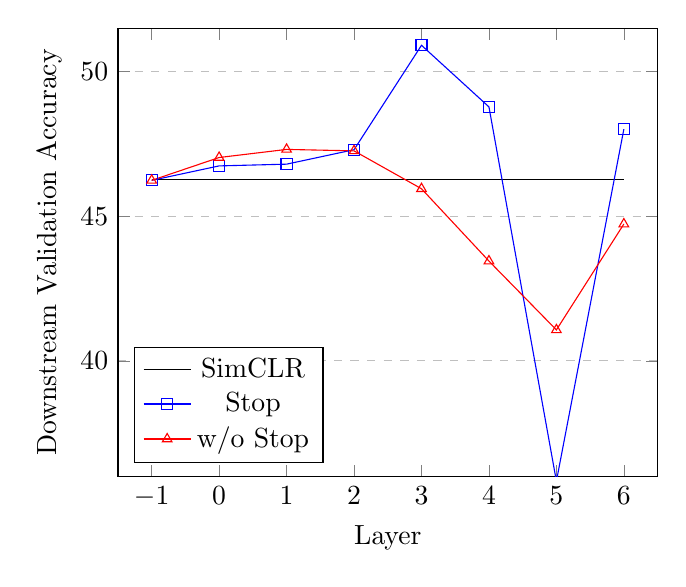
\begin{tikzpicture}
\begin{axis}[
    %title={Temperature dependence of CuSO\(_4\cdot\)5H\(_2\)O solubility},
    % width=0.8\textwidth,
    % height=0.5\textwidth,
    xlabel={Layer},
    ylabel={Downstream Validation Accuracy},
    xmin=-1.5, xmax=6.5,
    ymin=36, ymax=51.5,
    xtick={-1,0,1,2,3,4,5,6,7}, %,11,12,13},
    ytick={40,45,50},
    %ytick={0,0.2,0.4,0.6,0.8,1.0}, %,0.6,0.7,0.8,0.9,1.0},
    legend pos=south west,
    ymajorgrids=true,
    grid style=dashed,
]
\addplot[
    color=black,
    %mark=diamond,
    ]
    coordinates {
    % (300,62.14999771118164)(600,63.15999984741211)(900,62.91999816894531)(1200,62.29999923706055)(1500,61.93000030517578)
    (-1,46.27000045776367)
    (0,46.27000045776367)
    (1,46.27000045776367)
    (2,46.27000045776367)
    (3,46.27000045776367)
    (4,46.27000045776367)
    (5,46.27000045776367)
    (6,46.27000045776367)
    
    };
    \addlegendentry{SimCLR}
\addplot[
    color=blue,
    mark=square,
    ]
    coordinates {
    (-1, 46.23999786376953)
    (0, 46.73999786376953)
    (1, 46.79999923706055)
    (2, 47.29999923706055)
    (3, 50.90999984741211)
    (4, 48.779998779296875)
    (5, 35.84000015258789)
    (6, 48.0099983215332)
    };
    \addlegendentry{Stop}
\addplot[
    color=red,
    mark=triangle,
    ]
    coordinates {
    (-1, 46.23999786376953)
    (0, 47.029998779296875)
    (1, 47.30999755859375)
    (2, 47.2599983215332)
    (3, 45.94999694824219)
    (4, 43.45000076293945)
    (5, 41.06999969482422)
    (6, 44.72999954223633)
    };
    \addlegendentry{w/o Stop}


\end{axis}
\end{tikzpicture}
}
%\vspace{-.1in}
%\caption{Continue CIFAR100-CIFAR100}
\caption{Finetuning on CIFAR100 of networks pre-trained on CIFAR10. Comparing SimCLR with Deep Augmentation with and without stop-gradient.}
\label{fig:CIFAR10-CIFAR100-domain}
%\vspace{-0.5cm}
\end{figure}

\begin{figure}[ht]
\centering
\resizebox{0.33\columnwidth}{!}{%
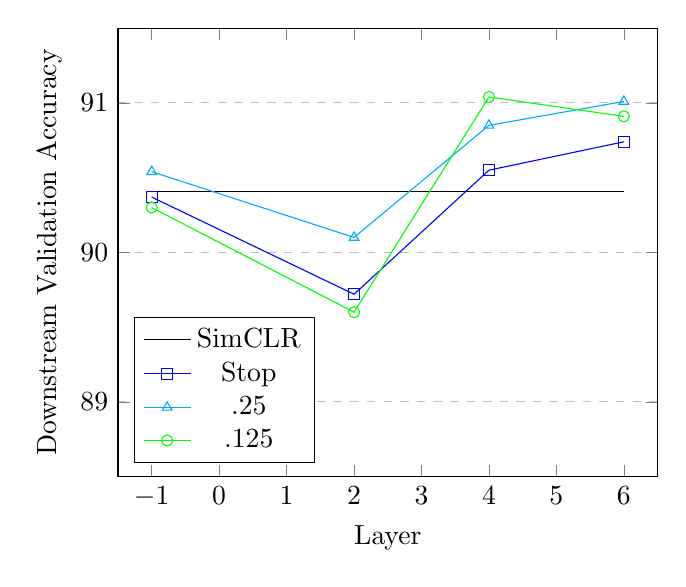
\begin{tikzpicture}
\begin{axis}[
    %title={Temperature dependence of CuSO\(_4\cdot\)5H\(_2\)O solubility},
    % width=0.8\textwidth,
    % height=0.5\textwidth,
    xlabel={Layer},
    ylabel={Downstream Validation Accuracy},
    xmin=-1.5, xmax=6.5,
    ymin=88.5, ymax=91.5,
    xtick={-1,0,1,2,3,4,5,6,7}, %,11,12,13},
    ytick={89,90,91},
    %ytick={0,0.2,0.4,0.6,0.8,1.0}, %,0.6,0.7,0.8,0.9,1.0},
    legend pos=south west,
    ymajorgrids=true,
    grid style=dashed,
]
\addplot[
    color=black,
    %mark=diamond,
    ]
    coordinates {
    % (300,62.14999771118164)(600,63.15999984741211)(900,62.91999816894531)(1200,62.29999923706055)(1500,61.93000030517578)
    (-1,90.40999603271484)
    (6,90.40999603271484)
    };
    \addlegendentry{SimCLR}
\addplot[
    color=blue,
    mark=square,
    ]
    coordinates {
    (-1, 90.3699951171875)
    %(0, 90.57999420166016)
    %(1, 90.43000030517578)
    (2, 89.72000122070312)
    %(3, 89.65999603271484)
    (4, 90.54999542236328)
    %(5, 89.1500015258789)
    (6, 90.73999786376953)
    };
    \addlegendentry{Stop}
% \addplot[
%     dashed,
%     mark options={solid},
%     color=blue,
%     mark=square,
%     ]
%     coordinates {
%     (-1,90.1199951171875)
%     (0, 90.25999450683594)
%     (1, 90.13999938964844)
%     (2, 89.91999816894531)
%     (3, 90.00999450683594)
%     (4, 91.29999542236328)
%     (5, 89.90999603271484)
%     (6, 91.32999420166016)
%     };
%     \addlegendentry{Stop*}
\addplot[
    mark options={solid},
    color=cyan,
    mark=triangle,
    ]
    coordinates {
    (-1, 90.54)
    (2, 90.10)
    (4, 90.85)
    (6, 91.01)
    };
    \addlegendentry{.25}

\addplot[
    mark options={solid},
    color=green,
    mark=o,
    ]
    coordinates {
    (-1, 90.30)
    (2, 89.60)
    (4, 91.04)
    (6, 90.91)
    };
    \addlegendentry{.125}


\end{axis}
\end{tikzpicture}
}
%\vspace{-.1in}
%\caption{Continue CIFAR100-CIFAR100}
\caption{CIFAR10: Comparing sampling 50\% of batch and applying dropout to that sample, with and without stop-gradient, for different dropout rates. ``Stop'' is short for stop-gradient.}
\label{fig:CIFAR10-compare-rates-N}
%\vspace{-0.5cm}
\end{figure}

% \subsection{Early Layers and Data Distribution}

% Early layers have fewer parameters to learn to be invariant to these transformations with respect to non-augmented images. This fools the network into believing the data-distribution is different from how it actually looks like at test time; the NN effectively never sees non-augmented data during training, and dropout is not creating realistic looking images as opposed to typical image transformations like cropping.

%Either way, training a NN with dropout should lead to less co-adaptation and in turn make higher layer transformations more useful. 
%This logic suggests that a NN trained with Deep Augmentation at a certain layer may be suitable for further training on a new dataset (optionally frozen up to that layer) using Deep Augmentation at the same layer.
%Future work may investigate ways to optimally train a NN so that dropout serves as a useful higher transformation. 
%}

\subsection{CIFAR100 across epochs}
\label{sec:CIFAR100-across-epochs}


We include results where we finetuned and tested checkpoints at different epochs for various experiments.

In Figure \ref{fig:CIFAR100-everywhere-vs-layer-epochs}, we include results for dropout everywhere at different rates and 50\% dropout at single layers. 

In Figure \ref{fig:CIFAR100-with-sg-without-sg-epochs}, we include results for sampling 50\% of each batch and performing 50\% dropout on that sample, with and without stop-gradient. 

In Figures \ref{fig:CIFAR100-with-sg-without-sg-epochs-PCA-1} and \ref{fig:CIFAR100-with-sg-without-sg-epochs-PCA-6}, we include results for sampling 50\% of each batch and subtracting the largest and sixth largest (respectively) principal component from that sample, with and without stop-gradient. 

In Figure \ref{fig:CIFAR100-freezingbeforeafter-epochs}, we compare freezing layers before or after Deep Augmentation with stop-gradient initialized with pre-trained SimCLR model. 

In Figure \ref{fig:continue-CIFAR100-epochs}, we inlcude results for 50\% sampling, 50\% dropout, with and without stop-gradient, and initialized with pre-trained SimCLR model.

\begin{figure}
\centering
\begin{subfigure}{.33\columnwidth}
\resizebox{\columnwidth}{!}{%
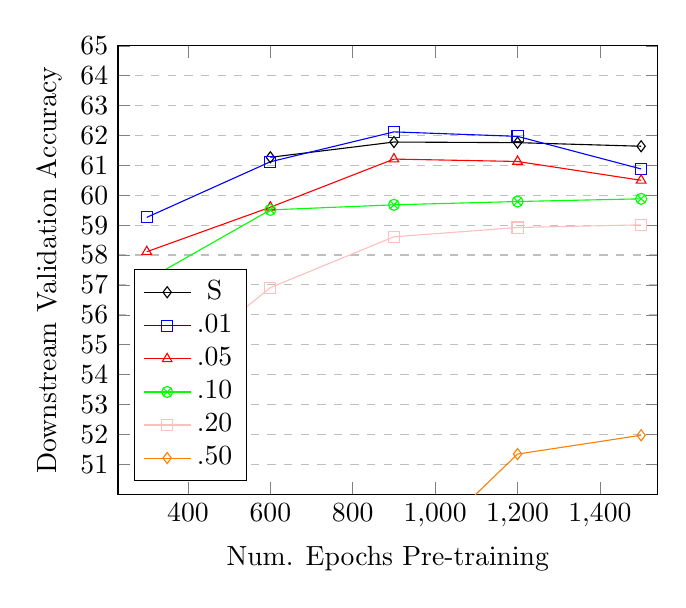
\begin{tikzpicture}
\begin{axis}[
    xlabel={Num. Epochs Pre-training},
    ylabel={Downstream Validation Accuracy},
    xmin=230, xmax=1540,
    ymin=50, ymax=65,
    xtick={200,400,600,800,1000,1200,1400}, %,11,12,13},
    ytick={51,52,53,54,55,56,57,58,59,60,61,62,63,64,65},
    %ytick={0,0.2,0.4,0.6,0.8,1.0}, %,0.6,0.7,0.8,0.9,1.0},
    legend pos=south west,
    ymajorgrids=true,
    grid style=dashed,
]
\addplot[
    color=black,
    mark=diamond,
    ]
    coordinates {
    (600,61.27)(900,61.78)(1200,61.76)(1500,61.64)
    };
    \addlegendentry{S}
\addplot[
    color=blue,
    mark=square,
    ]
    coordinates {
   (300,59.2599983215332)(600,61.119998931884766)(900,62.119998931884766)(1200,61.96999740600586)(1500,60.87999725341797)
    };
    \addlegendentry{.01}
\addplot[
    color=red,
    mark=triangle,
    ]
    coordinates {
    (300,58.1099967956543)(600,59.599998474121094)(900,61.209999084472656)(1200,61.12999725341797)(1500,60.5)
    };
    \addlegendentry{.05}
\addplot[
    color=green,
    mark=otimes,
    ]
    coordinates {
    (300,57.15999984741211)(600,59.5099983215332)(900,59.68000030517578)(1200,59.78999710083008)(1500,59.87999725341797)
    };
    \addlegendentry{.10}
\addplot[
    color=pink,
    mark=square,
    ]
    coordinates {
    (300,53.54999923706055)(600,56.90999984741211)(900,58.6099967956543)(1200,58.91999816894531)(1500,59.0099983215332)
    };
    \addlegendentry{.20}
\addplot[
    color=orange,
    mark=diamond,
    ]
    coordinates {
    (300,37.86000061035156)(600,43.47999954223633)(900,47.349998474121094)(1200,51.34000015258789)(1500,51.96999740600586)
    };
    \addlegendentry{.50}


\end{axis}
\end{tikzpicture}
}
%\vspace{-.1in}
\caption{Dropout at all layers}
\label{fig:drop_everywhere_CIFAR100} 
\end{subfigure}%
\hspace{0.2in}
\begin{subfigure}{.33\columnwidth}
\centering
\resizebox{\columnwidth}{!}{%
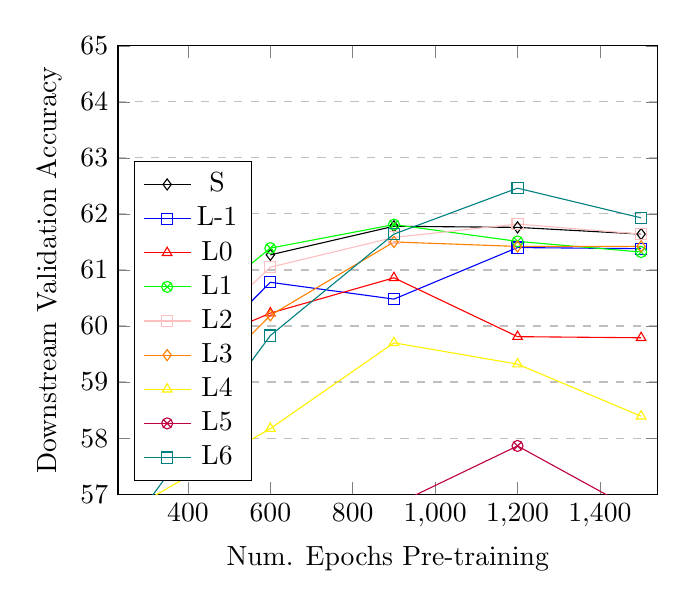
\begin{tikzpicture}
\begin{axis}[
    %title={Temperature dependence of CuSO\(_4\cdot\)5H\(_2\)O solubility},
    % width=0.8\textwidth,
    % height=0.5\textwidth,
    xlabel={Num. Epochs Pre-training},
    ylabel={Downstream Validation Accuracy},
    xmin=230, xmax=1540,
    ymin=57, ymax=65,
    xtick={200,400,600,800,1000,1200,1400}, %,11,12,13},
    ytick={57, 58, 59, 60, 61, 62, 63, 64, 65},
    %ytick={0,0.2,0.4,0.6,0.8,1.0}, %,0.6,0.7,0.8,0.9,1.0},
    legend pos=south west,
    ymajorgrids=true,
    grid style=dashed,
]
\addplot[
    color=black,
    mark=diamond,
    ]
    coordinates {
    (600,61.27)(900,61.78)(1200,61.76)(1500,61.64)
    };
    \addlegendentry{S}

\addplot[
    color=blue,
    mark=square,
    ]
    coordinates {
    (300,58.55999755859375)(600,60.779998779296875)(900,60.47999954223633)(1200,61.39999771118164)(1500,61.37999725341797)
    };
    \addlegendentry{L-1}
\addplot[
    color=red,
    mark=triangle,
    ]
    coordinates {
    (300,59.28999710083008)(600,60.22999954223633)(900,60.8599967956543)(1200,59.80999755859375)(1500,59.78999710083008)
    };
    
    \addlegendentry{L0}
\addplot[
    color=green,
    mark=otimes,
    ]
    coordinates {
    (300,59.59000015258789)(600,61.38999938964844)(900,61.80999755859375)(1200,61.5099983215332)(1500,61.31999969482422)
    };
    
    \addlegendentry{L1}
\addplot[
    color=pink,
    mark=square,
    ]
    coordinates {
    (300,58.94999694824219)(600,61.04999923706055)(900,61.57999801635742)(1200,61.81999969482422)(1500,61.63999938964844)
    
    };
    \addlegendentry{L2}
\addplot[
    color=orange,
    mark=diamond,
    ]
    coordinates {
    (300,57.959999084472656)(600,60.189998626708984)(900,61.5)(1200,61.41999816894531)(1500,61.41999816894531)
    };
    \addlegendentry{L3}
    
\addplot[
    color=yellow,
    mark=triangle,
    ]
    coordinates {
    (300,56.88999938964844)(600,58.16999816894531)(900,59.69999694824219)(1200,59.31999969482422)(1500,58.38999938964844)
    
    };
    \addlegendentry{L4}
\addplot[
    color=purple,
    mark=otimes,
    ]
    coordinates {
    (300,52.099998474121094)(600,55.30999755859375)(900,56.79999923706055)(1200,57.8599967956543)(1500,56.64999771118164)
    };
    
    \addlegendentry{L5}
\addplot[
    color=teal,
    mark=square,
    ]
    coordinates {
    (300,56.84000015258789)(600,59.82999801635742)(900,61.63999938964844)(1200,62.459999084472656)(1500,61.93000030517578)
    };
    \addlegendentry{L6}

\end{axis}
\end{tikzpicture}
}
%\vspace{-.1in}
\caption{50\% dropout at single layer}
\label{fig:trainble-two-sided-CIFAR100}
\end{subfigure}
\caption{CIFAR100. Comparing dropout rates at all layers versus 50\% dropout targeted at a specific layer. Note difference in $y$-axis.}
\label{fig:CIFAR100-everywhere-vs-layer-epochs}
\end{figure}

\begin{figure}
\centering
\begin{subfigure}{.33\columnwidth}
\resizebox{\columnwidth}{!}{%
\begin{tikzpicture}
\begin{axis}[
    %title={Temperature dependence of CuSO\(_4\cdot\)5H\(_2\)O solubility},
    % width=0.8\textwidth,
    % height=0.5\textwidth,
    xlabel={Num. Epochs Pre-training},
    ylabel={Downstream Validation Accuracy},
    xmin=230, xmax=1540,
    ymin=57, ymax=65,
    xtick={200,400,600,800,1000,1200,1400}, %,11,12,13},
    ytick={57, 58, 59, 60, 61, 62, 63, 64, 65},
    %ytick={0,0.2,0.4,0.6,0.8,1.0}, %,0.6,0.7,0.8,0.9,1.0},
    legend pos=south west,
    ymajorgrids=true,
    grid style=dashed,
]
\addplot[
    color=black,
    mark=diamond,
    ]
    coordinates {
    (600,61.27)(900,61.78)(1200,61.76)(1500,61.64)
    };
    \addlegendentry{S}
\addplot[
    color=blue,
    mark=square,
    ]
    coordinates {
    (600,60.959999084472656)(900,62.39999771118164)(1200,61.12999725341797)(1500,61.43000030517578)
    };
    \addlegendentry{L-1}
\addplot[
    color=red,
    mark=triangle,
    ]
    coordinates {
    (600,60.62999725341797)(900,62.15999984741211)(1200,61.48999786376953)(1500,61.269996643066406)
    };
    \addlegendentry{L0}
\addplot[
    color=green,
    mark=otimes,
    ]
    coordinates {
    (600,61.1099967956543)(900,61.68000030517578)(1200,61.13999938964844)(1500,61.38999938964844)
    };
    \addlegendentry{L1}
\addplot[
    color=pink,
    mark=square,
    ]
    coordinates {
    (600,60.09000015258789)(900,60.54999923706055)(1200,61.06999969482422)(1500,61.94999694824219)
    };
    \addlegendentry{L2}
\addplot[
    color=orange,
    mark=diamond,
    ]
    coordinates {
    (600,57.41999816894531)(900,59.099998474121094)(1200,61.29999923706055)(1500,62.43000030517578)
    };
    \addlegendentry{L3}
\addplot[
    color=yellow,
    mark=triangle,
    ]
    coordinates {
    (600,59.96999740600586)(900,61.25)(1200,63.53999710083008)(1500,63.39999771118164)
    };
    \addlegendentry{L4}
\addplot[
    color=purple,
    mark=otimes,
    ]
    coordinates {
    (600,56.64999771118164)(900,57.21999740600586)(1200,58.689998626708984)(1500,58.59000015258789)
    };
    \addlegendentry{L5}
\addplot[
    color=teal,
    mark=square,
    ]
    coordinates {
    (600,58.209999084472656)(900,62.029998779296875)(1200,63.849998474121094)(1500,62.959999084472656)
    };
    \addlegendentry{L6}
% \addplot[
%     color=green,
%     mark=square,
%     ]
%     coordinates {
%     (300,55.84000015258789)(600,59.32999801635742)(900,61.41999816894531)(1200,62.869998931884766)(1500,63.56999969482422)
%     };
%     \addlegendentry{L4L6}

% \addplot[
%     color=brown,
%     mark=square,
%     ]
%     coordinates {
%     (300,56.28999710083008)(600,59.189998626708984)(900,62.6099967956543)(1200,62.82999801635742)(1500,62.89999771118164)
%     };
%     \addlegendentry{L4}

    

\end{axis}
\end{tikzpicture}
%\vspace{-.1in}

}
\caption{With stop-gradient}
\label{fig:CIFAR100-CIFAR100}
\end{subfigure}%
\hspace{0.2in}
\begin{subfigure}{.33\columnwidth}
\centering
\resizebox{\columnwidth}{!}{%
\begin{tikzpicture}
\begin{axis}[
    %title={Temperature dependence of CuSO\(_4\cdot\)5H\(_2\)O solubility},
    % width=0.8\textwidth,
    % height=0.5\textwidth,
    xlabel={Num. Epochs Pre-training},
    ylabel={Downstream Validation Accuracy},
    xmin=230, xmax=1540,
    ymin=57, ymax=65,
    xtick={200,400,600,800,1000,1200,1400}, %,11,12,13},
    ytick={57, 58, 59, 60, 61, 62, 63, 64, 65},
    %ytick={0,0.2,0.4,0.6,0.8,1.0}, %,0.6,0.7,0.8,0.9,1.0},
    legend pos=south west,
    ymajorgrids=true,
    grid style=dashed,
]
\addplot[
    color=black,
    mark=diamond,
    ]
    coordinates {
    (600,61.27)(900,61.78)(1200,61.76)(1500,61.64)
    };
    \addlegendentry{S}
\addplot[
    color=blue,
    mark=square,
    ]
    coordinates {
    (600,60.959999084472656)(900,62.39999771118164)(1200,61.12999725341797)(1500,61.43000030517578)
    };
    \addlegendentry{L-1}
\addplot[
    color=red,
    mark=triangle,
    ]
    coordinates {
    (600,61.619998931884766)(900,62.269996643066406)(1200,62.099998474121094)(1500,62.029998779296875)
    };
    \addlegendentry{L0}
\addplot[
    color=green,
    mark=otimes,
    ]
    coordinates {
    (600,60.959999084472656)(900,62.69999694824219)(1200,61.37999725341797)(1500,62.13999938964844)
    };
    \addlegendentry{L1}
\addplot[
    color=pink,
    mark=square,
    ]
    coordinates {
    (600,61.019996643066406)(900,62.28999710083008)(1200,61.84000015258789)(1500,61.769996643066406)
    };
    \addlegendentry{L2}
\addplot[
    color=orange,
    mark=diamond,
    ]
    coordinates {
    (600,60.54999923706055)(900,62.119998931884766)(1200,61.32999801635742)(1500,61.07999801635742)
    };
    \addlegendentry{L3}
\addplot[
    color=yellow,
    mark=triangle,
    ]
    coordinates {
    (600,58.93000030517578)(900,59.89999771118164)(1200,59.91999816894531)(1500,59.519996643066406)
    };
    \addlegendentry{L4}
\addplot[
    color=purple,
    mark=otimes,
    ]
    coordinates {
    (600,57.84000015258789)(900,58.47999954223633)(1200,58.81999969482422)(1500,57.16999816894531)
    };
    \addlegendentry{L5}
\addplot[
    color=teal,
    mark=square,
    ]
    coordinates {
    (600,60.46999740600586)(900,62.09000015258789)(1200,62.72999954223633)(1500,61.73999786376953)
    };
    \addlegendentry{L6}

% \addplot[
%     color=teal,
%     mark=square,
%     ]
%     coordinates {
%     (300,58.599998474121094)(600,61.279998779296875)(900,62.62999725341797)(1200,62.14999771118164)(1500,61.91999816894531)
%     };
%     \addlegendentry{L6}

    

\end{axis}
\end{tikzpicture}
%\vspace{-.1in}

}
%\vspace{-.1in}
\caption{Without stop-gradient}
\label{fig:trainble-CIFAR100-CIFAR100}
\end{subfigure}
\caption{CIFAR100. Comparing sampling 50\% and applying 50\% dropout, with or without stop-gradient.}
\label{fig:CIFAR100-with-sg-without-sg-epochs}
\end{figure}



\begin{figure}
\centering
\begin{subfigure}{.33\columnwidth}
\resizebox{\columnwidth}{!}{%
\begin{tikzpicture}
\begin{axis}[
    %title={Temperature dependence of CuSO\(_4\cdot\)5H\(_2\)O solubility},
    % width=0.8\textwidth,
    % height=0.5\textwidth,
    xlabel={Num. Epochs Pre-training},
    ylabel={Downstream Validation Accuracy},
    xmin=230, xmax=1540,
    ymin=57, ymax=65,
    xtick={200,400,600,800,1000,1200,1400}, %,11,12,13},
    ytick={57, 58, 59, 60, 61, 62, 63, 64, 65},
    %ytick={0,0.2,0.4,0.6,0.8,1.0}, %,0.6,0.7,0.8,0.9,1.0},
    legend pos=south west,
    ymajorgrids=true,
    grid style=dashed,
]
\addplot[
    color=black,
    mark=diamond,
    ]
    coordinates {
    (600,61.27)(900,61.78)(1200,61.76)(1500,61.64)
    };
    \addlegendentry{S}
\addplot[
    color=blue,
    mark=square,
    ]
    coordinates {
    (300, 59.16)(600, 61.96)(900, 61.78)(1200, 61.33)(1500, 61.57)
    };
    \addlegendentry{L-1}
\addplot[
    color=red,
    mark=triangle,
    ]
    coordinates {
    (300, 60.16)(600, 61.49)(900, 62.57)(1200, 61.81)(1500, 62.48)
    };
    \addlegendentry{L0}
\addplot[
    color=green,
    mark=otimes,
    ]
    coordinates {
    (300, 58.94)(600, 60.95)(900, 61.59)(1200, 62.45)(1500, 61.78)
    };
    \addlegendentry{L1}
\addplot[
    color=pink,
    mark=square,
    ]
    coordinates {
    (300, 59.47)(600, 59.51)(900, 60.95)(1200, 61.63)(1500, 61.66)
    };
    \addlegendentry{L2}
\addplot[
    color=orange,
    mark=diamond,
    ]
    coordinates {
    (300, 56.42)(600, 58.75)(900, 60.47)(1200, 62.17)(1500, 62.48)
    };
    \addlegendentry{L3}
\addplot[
    color=yellow,
    mark=triangle,
    ]
    coordinates {
    (300, 54.32)(600, 59.02)(900, 61.92)(1200, 62.58)(1500, 62.35)
    };
    \addlegendentry{L4}
\addplot[
    color=purple,
    mark=otimes,
    ]
    coordinates {
    (300, 54.11)(600, 58.57)(900, 61.12)(1200, 62.11)(1500, 62.1)
    };
    \addlegendentry{L5}
\addplot[
    color=teal,
    mark=square,
    ]
    coordinates {
    (300, 55.69)(600, 58.33)(900, 61.28)(1200, 63.01)(1500, 62.85)
    };
    \addlegendentry{L6}
\end{axis}
\end{tikzpicture}
%\vspace{-.1in}

}
\caption{With stop-gradient}
\label{fig:CIFAR100-CIFAR100}
\end{subfigure}%
\hspace{0.2in}
\begin{subfigure}{.33\columnwidth}
\centering
\resizebox{\columnwidth}{!}{%
\begin{tikzpicture}
\begin{axis}[
    %title={Temperature dependence of CuSO\(_4\cdot\)5H\(_2\)O solubility},
    % width=0.8\textwidth,
    % height=0.5\textwidth,
    xlabel={Num. Epochs Pre-training},
    ylabel={Downstream Validation Accuracy},
    xmin=230, xmax=1540,
    ymin=57, ymax=65,
    xtick={200,400,600,800,1000,1200,1400}, %,11,12,13},
    ytick={57, 58, 59, 60, 61, 62, 63, 64, 65},
    %ytick={0,0.2,0.4,0.6,0.8,1.0}, %,0.6,0.7,0.8,0.9,1.0},
    legend pos=south west,
    ymajorgrids=true,
    grid style=dashed,
]
\addplot[
    color=black,
    mark=diamond,
    ]
    coordinates {
    (600,61.27)(900,61.78)(1200,61.76)(1500,61.64)
    };
    \addlegendentry{S}
\addplot[
    color=blue,
    mark=square,
    ]
    coordinates {
    (300, 59.16)(600, 61.96)(900, 61.78)(1200, 61.33)(1500, 61.57)
    };
    \addlegendentry{L-1}
\addplot[
    color=red,
    mark=triangle,
    ]
    coordinates {
    (300, 59.92)(600, 61.12)(900, 62.68)(1200, 62.71)(1500, 62.25)
    };
    \addlegendentry{L0}
\addplot[
    color=green,
    mark=otimes,
    ]
    coordinates {
    (300, 60.14)(600, 61.69)(900, 62.1)(1200, 61.64)(1500, 61.71)
    };
    \addlegendentry{L1}
\addplot[
    color=pink,
    mark=square,
    ]
    coordinates {
    (300, 58.47)(600, 61.17)(900, 61.11)(1200, 61.1)(1500, 61.43)
    };
    \addlegendentry{L2}
\addplot[
    color=orange,
    mark=diamond,
    ]
    coordinates {
    (300, 59.18)(600, 61.24)(900, 61.83)(1200, 61.54)(1500, 61.86)
    };
    \addlegendentry{L3}
\addplot[
    color=yellow,
    mark=triangle,
    ]
    coordinates {
    (300, 60.46)(600, 62.03)(900, 62.01)(1200, 61.35)(1500, 61.62)
    };
    \addlegendentry{L4}
\addplot[
    color=purple,
    mark=otimes,
    ]
    coordinates {
    (300, 59.58)(600, 61.39)(900, 62.85)(1200, 61.56)(1500, 61.5)
    };
    \addlegendentry{L5}
\addplot[
    color=teal,
    mark=square,
    ]
    coordinates {
    (300, 22.17)(600, 13.1)(900, 8.15)(1200, 7.1)(1500, 9.85) 
    };
    \addlegendentry{L6}
\end{axis}
\end{tikzpicture}
%\vspace{-.1in}
}
%\vspace{-.1in}
\caption{Without stop-gradient}
\label{fig:trainble-CIFAR100-CIFAR100-pca1}
\end{subfigure}
\caption{PCA CIFAR100: Comparing sampling 50\% of batch and subtracting the largest principal component from that sample, with and without stop-gradient.}
\label{fig:CIFAR100-with-sg-without-sg-epochs-PCA-1}
\end{figure}

\begin{figure}
\centering
\begin{subfigure}{.33\columnwidth}
\resizebox{\columnwidth}{!}{%
\begin{tikzpicture}
\begin{axis}[
    %title={Temperature dependence of CuSO\(_4\cdot\)5H\(_2\)O solubility},
    % width=0.8\textwidth,
    % height=0.5\textwidth,
    xlabel={Num. Epochs Pre-training},
    ylabel={Downstream Validation Accuracy},
    xmin=230, xmax=1540,
    ymin=57, ymax=65,
    xtick={200,400,600,800,1000,1200,1400}, %,11,12,13},
    ytick={57, 58, 59, 60, 61, 62, 63, 64, 65},
    %ytick={0,0.2,0.4,0.6,0.8,1.0}, %,0.6,0.7,0.8,0.9,1.0},
    legend pos=south west,
    ymajorgrids=true,
    grid style=dashed,
]
\addplot[
    color=black,
    mark=diamond,
    ]
    coordinates {
    (600,61.27)(900,61.78)(1200,61.76)(1500,61.64)
    };
    \addlegendentry{S}
\addplot[
    color=blue,
    mark=square,
    ]
    coordinates {
    (300, 60.08)(600, 62.47)(900, 62.89)(1200, 62.38)(1500, 62.74)
    };
    \addlegendentry{L-1}
\addplot[
    color=red,
    mark=triangle,
    ]
    coordinates {
    (300, 58.56)(600, 61.07)(900, 52.25)(1200, 53.45)(1500, 62.22)
    };
    \addlegendentry{L0}
\addplot[
    color=green,
    mark=otimes,
    ]
    coordinates {
    (300, 58.61)(600, 61.15)(900, 58.91)(1200, 61.3)(1500, 61.8)
    };
    \addlegendentry{L1}
\addplot[
    color=pink,
    mark=square,
    ]
    coordinates {
    (300, 55.71)(600, 59.33)(900, 58.98)(1200, 60.03)(1500, 60.26)
    };
    \addlegendentry{L2}
\addplot[
    color=orange,
    mark=diamond,
    ]
    coordinates {
    (300, 54.22)(600, 55.04)(900, 57.85)(1200, 61.09)(1500, 63.04)
    };
    \addlegendentry{L3}
\addplot[
    color=yellow,
    mark=triangle,
    ]
    coordinates {
    (300, 54.69)(600, 58.73)(900, 61.7)(1200, 62.93)(1500, 62.82)
    };
    \addlegendentry{L4}
\addplot[
    color=purple,
    mark=otimes,
    ]
    coordinates {
    (300, 53.96)(600, 58.81)(900, 61.09)(1200, 62.71)(1500, 62.78)
    };
    \addlegendentry{L5}
\addplot[
    color=teal,
    mark=square,
    ]
    coordinates {
    (300, 55.49)(600, 59.02)(900, 61.07)(1200, 62.89)(1500, 63.46)
    };
    \addlegendentry{L6}
\end{axis}
\end{tikzpicture}
%\vspace{-.1in}

}
\caption{With stop-gradient}
\label{fig:CIFAR100-CIFAR100}
\end{subfigure}%
\hspace{0.2in}
\begin{subfigure}{.33\columnwidth}
\centering
\resizebox{\columnwidth}{!}{%
\begin{tikzpicture}
\begin{axis}[
    %title={Temperature dependence of CuSO\(_4\cdot\)5H\(_2\)O solubility},
    % width=0.8\textwidth,
    % height=0.5\textwidth,
    xlabel={Num. Epochs Pre-training},
    ylabel={Downstream Validation Accuracy},
    xmin=230, xmax=1540,
    ymin=57, ymax=65,
    xtick={200,400,600,800,1000,1200,1400}, %,11,12,13},
    ytick={57, 58, 59, 60, 61, 62, 63, 64, 65},
    %ytick={0,0.2,0.4,0.6,0.8,1.0}, %,0.6,0.7,0.8,0.9,1.0},
    legend pos=south west,
    ymajorgrids=true,
    grid style=dashed,
]
\addplot[
    color=black,
    mark=diamond,
    ]
    coordinates {
    (600,61.27)(900,61.78)(1200,61.76)(1500,61.64)
    };
    \addlegendentry{S}
\addplot[
    color=blue,
    mark=square,
    ]
    coordinates {
    (300, 60.08)(600, 62.47)(900, 62.89)(1200, 62.38)(1500, 62.74)
    };
    \addlegendentry{L-1}
\addplot[
    color=red,
    mark=triangle,
    ]
    coordinates {
    (300, 60.48)(600, 61.23)(900, 62.11)(1200, 62.01)(1500, 62.31)
    };
    \addlegendentry{L0}
\addplot[
    color=green,
    mark=otimes,
    ]
    coordinates {
    (300, 59.55)(600, 61.96)(900, 62.83)(1200, 62.24)(1500, 61.05)
    };
    \addlegendentry{L1}
\addplot[
    color=pink,
    mark=square,
    ]
    coordinates {
    (300, 59.98)(600, 61.15)(900, 63.02)(1200, 61.96)(1500, 62.12)
    };
    \addlegendentry{L2}
\addplot[
    color=orange,
    mark=diamond,
    ]
    coordinates {
    (300, 58.99)(600, 60.76)(900, 62.28)(1200, 61.48)(1500, 61.53)
    };
    \addlegendentry{L3}
\addplot[
    color=yellow,
    mark=triangle,
    ]
    coordinates {
    (300, 53.98)(600, 56)(900, 59.44)(1200, 59.85)(1500, 61.78)
    };
    \addlegendentry{L4}
\addplot[
    color=purple,
    mark=otimes,
    ]
    coordinates {
    (300, 24.47)(600, 19.78)(900, 20.59)(1200, 14.33)(1500, 25.06)
    };
    \addlegendentry{L5}
\addplot[
    color=teal,
    mark=square,
    ]
    coordinates {
    (300, 49.53)(600, 57.39)(900, 60.02)(1200, 62.75)(1500, 62.6)
    };
    \addlegendentry{L6}
\end{axis}
\end{tikzpicture}
%\vspace{-.1in}
}
%\vspace{-.1in}
\caption{Without stop-gradient}
\label{fig:trainble-CIFAR100-CIFAR100-pca1}
\end{subfigure}
\caption{PCA CIFAR100: Comparing sampling 50\% of batch and subtracting the sixth largest principal component from that sample, with and without stop-gradient.}
\label{fig:CIFAR100-with-sg-without-sg-epochs-PCA-6}
\end{figure}



\begin{figure}
\centering
\begin{subfigure}{.33\columnwidth}
  \centering
  \resizebox{1.0\columnwidth}{!}{
  \begin{tikzpicture}
\begin{axis}[
    %title={Temperature dependence of CuSO\(_4\cdot\)5H\(_2\)O solubility},
    % width=0.8\textwidth,
    % height=0.5\textwidth,
    xlabel={Num. Epochs Pre-training},
    ylabel={Downstream Validation Accuracy},
    xmin=230, xmax=1540,
    ymin=57, ymax=65,
    xtick={200,400,600,800,1000,1200,1400}, %,11,12,13},
    ytick={57, 58, 59, 60, 61, 62, 63, 64, 65},
    %ytick={0,0.2,0.4,0.6,0.8,1.0}, %,0.6,0.7,0.8,0.9,1.0},
    legend pos=south west,
    ymajorgrids=true,
    grid style=dashed,
]
\addplot[
    color=black,
    mark=diamond,
    ]
    coordinates {
    (300,62.79999923706055)(600,62.5)(900,62.87999725341797)(1200,62.28999710083008)(1500,61.91999816894531)
    };
    \addlegendentry{S}
\addplot[
    color=blue,
    mark=square,
    ]
    coordinates {
    (600,61.94999694824219)(900,62.209999084472656)(1200,61.939998626708984)(1500,61.66999816894531)
    %(300,60.39999771118164)(600,61.98999786376953)(900,62.3599967956543)(1200,61.73999786376953)(1500,61.7599983215332)
    };
    \addlegendentry{L-1}
\addplot[
    color=red,
    mark=triangle,
    ]
    coordinates {
    (300,62.189998626708984)(600,62.2599983215332)(900,61.98999786376953)(1200,62.07999801635742)(1500,61.38999938964844)
    %(300,61.03999710083008)(600,62.3599967956543)(900,62.1099967956543)(1200,62.43000030517578)(1500,61.769996643066406)
    
    };
    \addlegendentry{L0}
\addplot[
    color=green,
    mark=otimes,
    ]
    coordinates {
    (300,61.81999969482422)(600,62.94999694824219)(900,63.56999969482422)(1200,62.25)(1500,61.779998779296875)
    %(300,62.28999710083008)(600,62.869998931884766)(900,63.439998626708984)(1200,63.09000015258789)(1500,62.0099983215332)
    
    };
    \addlegendentry{L1}
\addplot[
    color=pink,
    mark=square,
    ]
    coordinates {
    (300,61.869998931884766)(600,63.279998779296875)(900,63.69999694824219)(1200,62.03999710083008)(1500,61.54999923706055)
    %(300,62.16999816894531)(600,62.959999084472656)(900,62.21999740600586)(1200,61.459999084472656)(1500,61.40999984741211)
    
    };
    \addlegendentry{L2}
\addplot[
    color=orange,
    mark=diamond,
    ]
    coordinates {
    (300,55.57999801635742)(600,55.46999740600586)(900,57.29999923706055)(1200,57.69999694824219)(1500,58.21999740600586)
    
    };
    \addlegendentry{L3}
\addplot[
    color=yellow,
    mark=triangle,
    ]
    coordinates {
    (300,59.97999954223633)(600,59.22999954223633)(900,60.439998626708984)(1200,60.79999923706055)(1500,61.209999084472656)
    
    };
    \addlegendentry{L4}
\addplot[
    color=purple,
    mark=otimes,
    ]
    coordinates {
    (300,59.30999755859375)(600,59.349998474121094)(900,59.84000015258789)(1200,60.90999984741211)(1500,61.349998474121094)
    
    };
    \addlegendentry{L5}
% \addplot[
%     color=teal,
%     mark=square,
%     ]
%     coordinates {
%     (300,59.599998474121094)(600,59.28999710083008)(900,60.30999755859375)(1200,60.63999938964844)(1500,61.07999801635742)
%     % (300,59.63999938964844)(600,60.80999755859375)(900,62.57999801635742)(1200,64.29000091552734)(1500,64.18999481201172)
%     };
%     \addlegendentry{25}

\end{axis}
\end{tikzpicture}
}
%\caption{Freeze Continue CIFAR100-CIFAR100}
\caption{Freeze layers before Deep Augmentation}
\label{fig:freeze-continue-CIFAR100-CIFAR100}
\end{subfigure}%
\hspace{0.2in}
\begin{subfigure}{.33\columnwidth}
  \centering
  \resizebox{1.0\columnwidth}{!}{
\centering
\begin{tikzpicture}
\begin{axis}[
    %title={Temperature dependence of CuSO\(_4\cdot\)5H\(_2\)O solubility},
    % width=0.8\textwidth,
    % height=0.5\textwidth,
    xlabel={Num. Epochs Pre-training},
    ylabel={Downstream Validation Accuracy},
    xmin=230, xmax=1540,
    ymin=57, ymax=65,
    xtick={200,400,600,800,1000,1200,1400}, %,11,12,13},
    ytick={57, 58, 59, 60, 61, 62, 63, 64, 65},
    %ytick={0,0.2,0.4,0.6,0.8,1.0}, %,0.6,0.7,0.8,0.9,1.0},
    legend pos=south west,
    ymajorgrids=true,
    grid style=dashed,
]
\addplot[
    color=black,
    mark=diamond,
    ]
    coordinates {
    (300,62.79999923706055)(600,62.5)(900,62.87999725341797)(1200,62.28999710083008)(1500,61.91999816894531)
    };
    \addlegendentry{S}
% \addplot[
%     color=blue,
%     mark=square,
%     ]
%     coordinates {
%     (600,61.94999694824219)(900,62.209999084472656)(1200,61.939998626708984)(1500,61.66999816894531)
%     };
%     \addlegendentry{L-1}
\addplot[
    color=red,
    mark=triangle,
    ]
    coordinates {
    (300,58.37999725341797)(600,58.30999755859375)(900,58.64999771118164)(1200,59.80999755859375)(1500,60.369998931884766)
    };
    \addlegendentry{L0}
\addplot[
    color=green,
    mark=otimes,
    ]
    coordinates {
    (300,59.38999938964844)(600,59.019996643066406)(900,59.8599967956543)(1200,60.28999710083008)(1500,61.3599967956543)
    };
    \addlegendentry{L1}
\addplot[
    color=pink,
    mark=square,
    ]
    coordinates {
    (300,58.68000030517578)(600,59.1099967956543)(900,60.16999816894531)(1200,61.06999969482422)(1500,61.90999984741211)
    };
    \addlegendentry{L2}
\addplot[
    color=orange,
    mark=diamond,
    ]
    coordinates {
    (300,58.519996643066406)(600,60.34000015258789)(900,59.689998626708984)(1200,61.209999084472656)(1500,61.69999694824219)
    };
    \addlegendentry{L3}
\addplot[
    color=yellow,
    mark=triangle,
    ]
    coordinates {
    (300,59.32999801635742)(600,60.05999755859375)(900,61.38999938964844)(1200,60.25)(1500,60.6099967956543)
    };
    \addlegendentry{L4}
\addplot[
    color=purple,
    mark=otimes,
    ]
    coordinates {
    (300,56.07999801635742)(600,56.53999710083008)(900,57.7599983215332)(1200,57.57999801635742)(1500,56.81999969482422)
    
    
    };
    \addlegendentry{L5}
% \addplot[
%     color=teal,
%     mark=square,
%     ]
%     coordinates {
%     (300,61.63999938964844)(600,61.97999954223633)(900,62.91999816894531)(1200,62.62999725341797)(1500,61.5099983215332)
%     };
%     \addlegendentry{L6}

\end{axis}
\end{tikzpicture}
}
%\vspace{-.1in}
%\caption{Continue Freeze Reverse CIFAR100-CIFAR100}
\caption{Freeze layers after Deep Augmentation}
\label{fig:freeze-reverse-continue-CIFAR100-CIFAR100}
\end{subfigure}
\caption{CIFAR100. Comparing freezing layers before or after Deep Augmentation with stop-gradient initialized with pre-trained SimCLR model.}
\label{fig:CIFAR100-freezingbeforeafter-epochs}
\end{figure}




\begin{figure}
\centering
\begin{subfigure}{.33\columnwidth}
  \centering
  \resizebox{1.0\columnwidth}{!}{
  \begin{tikzpicture}
\begin{axis}[
    %title={Temperature dependence of CuSO\(_4\cdot\)5H\(_2\)O solubility},
    % width=0.8\textwidth,
    % height=0.5\textwidth,
    xlabel={Num. Epochs Pre-training},
    ylabel={Downstream Validation Accuracy},
    xmin=230, xmax=1540,
    ymin=57, ymax=65,
    xtick={200,400,600,800,1000,1200,1400}, %,11,12,13},
    ytick={57, 58, 59, 60, 61, 62, 63, 64, 65},
    %ytick={0,0.2,0.4,0.6,0.8,1.0}, %,0.6,0.7,0.8,0.9,1.0},
    legend pos=south west,
    ymajorgrids=true,
    grid style=dashed,
]
\addplot[
    color=black,
    mark=diamond,
    ]
    coordinates {
    % (300,62.14999771118164)(600,63.15999984741211)(900,62.91999816894531)(1200,62.29999923706055)(1500,61.93000030517578)
    (300,62.79999923706055)(600,62.5)(900,62.87999725341797)(1200,62.28999710083008)(1500,61.91999816894531)
    };
    \addlegendentry{S}
\addplot[
    color=blue,
    mark=square,
    ]
    coordinates {
    (600,61.94999694824219)(900,62.209999084472656)(1200,61.939998626708984)(1500,61.66999816894531)
    %(300,60.39999771118164)(600,61.98999786376953)(900,62.3599967956543)(1200,61.73999786376953)(1500,61.7599983215332)
    };
    \addlegendentry{L-1}
\addplot[
    color=red,
    mark=triangle,
    ]
    coordinates {
    (600,62.12999725341797)(900,62.13999938964844)(1200,61.619998931884766)(1500,61.47999954223633)
    %(300,60.779998779296875)(600,61.3599967956543)(900,62.15999984741211)(1200,61.119998931884766)(1500,60.91999816894531)
    };
    \addlegendentry{L0}
\addplot[
    color=green,
    mark=otimes,
    ]
    coordinates {
    (600,61.5099983215332)(900,62.209999084472656)(1200,62.3599967956543)(1500,61.939998626708984)
    %(300,60.119998931884766)(600,61.30999755859375)(900,62.769996643066406)(1200,61.619998931884766)(1500,61.80999755859375)
    };
    
    \addlegendentry{L1}
\addplot[
    color=pink,
    mark=square,
    ]
    coordinates {
    (300,59.72999954223633)(600,60.269996643066406)(900,61.14999771118164)(1200,61.44999694824219)(1500,62.0099983215332)
    %(300,59.72999954223633)(600,60.269996643066406)(900,61.14999771118164)(1200,61.44999694824219)(1500,62.0099983215332)
    };
    \addlegendentry{L2}
\addplot[
    color=orange,
    mark=diamond,
    ]
    coordinates {
    (300,57.94999694824219)(600,58.459999084472656)(900,60.71999740600586)(1200,62.75)(1500,62.93000030517578)
    };
    \addlegendentry{L3}
\addplot[
    color=yellow,
    mark=triangle,
    ]
    coordinates {
    (300,59.869998931884766)(600,61.72999954223633)(900,62.2599983215332)(1200,64.22000122070312)(1500,64.0999984741211)
    };
    \addlegendentry{L4}
\addplot[
    color=purple,
    mark=otimes,
    ]
    coordinates {
    (300,58.07999801635742)(600,58.869998931884766)(900,59.869998931884766)(1200,60.18000030517578)(1500,60.09000015258789)
    };
    \addlegendentry{L5}
\addplot[
    color=teal,
    mark=square,
    ]
    coordinates {
    (300,59.63999938964844)(600,60.80999755859375)(900,62.57999801635742)(1200,64.29000091552734)(1500,64.18999481201172)
    };
    \addlegendentry{L6}

\end{axis}
\end{tikzpicture}
}
\caption{With stop-gradient.}
\label{fig:continue-CIFAR100-CIFAR100}
\end{subfigure}%
\hspace{0.2in}
\begin{subfigure}{.33\columnwidth}
  \centering
  \resizebox{1.0\columnwidth}{!}{
\centering
\begin{tikzpicture}
\begin{axis}[
    %title={Temperature dependence of CuSO\(_4\cdot\)5H\(_2\)O solubility},
    % width=0.8\textwidth,
    % height=0.5\textwidth,
    xlabel={Num. Epochs},
    ylabel={Downstream Validation Accuracy},
    xmin=230, xmax=1540,
    ymin=57, ymax=64,
    xtick={200,400,600,800,1000,1200,1400}, %,11,12,13},
    ytick={57, 58, 59, 60, 61, 62, 63, 64},
    %ytick={0,0.2,0.4,0.6,0.8,1.0}, %,0.6,0.7,0.8,0.9,1.0},
    legend pos=south west,
    ymajorgrids=true,
    grid style=dashed,
]
\addplot[
    color=black,
    mark=diamond,
    ]
    coordinates {
    (300,62.79999923706055)(600,62.5)(900,62.87999725341797)(1200,62.28999710083008)(1500,61.91999816894531)
    };
    \addlegendentry{S}
\addplot[
    color=blue,
    mark=square,
    ]
    coordinates {
    (600,61.94999694824219)(900,62.209999084472656)(1200,61.939998626708984)(1500,61.66999816894531)
    };
    \addlegendentry{L-1}
\addplot[
    color=red,
    mark=triangle,
    ]
    coordinates {
    (300,61.91999816894531)(600,62.54999923706055)(900,62.39999771118164)(1200,61.959999084472656)(1500,61.59000015258789)
    };
    \addlegendentry{L0}
\addplot[
    color=green,
    mark=otimes,
    ]
    coordinates {
    (300,62.59000015258789)(600,62.69999694824219)(900,62.32999801635742)(1200,62.19999694824219)(1500,61.55999755859375)
    };
    \addlegendentry{L1}
\addplot[
    color=pink,
    mark=square,
    ]
    coordinates {
    (300,61.709999084472656)(600,62.81999969482422)(900,62.80999755859375)(1200,61.73999786376953)(1500,61.849998474121094)
    };
    \addlegendentry{L2}
\addplot[
    color=orange,
    mark=diamond,
    ]
    coordinates {
    (300,62.12999725341797)(600,62.2599983215332)(900,62.189998626708984)(1200,62.56999969482422)(1500,62.21999740600586)
    };
    \addlegendentry{L3}
\addplot[
    color=yellow,
    mark=triangle,
    ]
    coordinates {
    (300,60.37999725341797)(600,59.93000030517578)(900,61.79999923706055)(1200,60.099998474121094)(1500,59.62999725341797)
    };
    \addlegendentry{L4}
\addplot[
    color=purple,
    mark=otimes,
    ]
    coordinates {
    (300,58.84000015258789)(600,58.529998779296875)(900,59.55999755859375)(1200,59.06999969482422)(1500,58.68000030517578)
    };
    \addlegendentry{L5}
\addplot[
    color=teal,
    mark=square,
    ]
    coordinates {
    (300,61.63999938964844)(600,61.97999954223633)(900,62.91999816894531)(1200,62.62999725341797)(1500,61.5099983215332)
    };
    \addlegendentry{L6}

\end{axis}
\end{tikzpicture}
%\vspace{-.1in}
}
\caption{Without stop-gradient.}
\label{fig:random_erdos}
\end{subfigure}
\caption{CIFAR100. 50\% sampling, 50\% dropout, with and without stop-gradient, and initialized with pre-trained SimCLR model.}
\label{fig:continue-CIFAR100-epochs}
\end{figure}

%%%%%%%%%%%%


\subsection{CIFAR10 across epochs}
\label{sec:CIFAR10-across-epochs}

We include results where we finetuned and tested checkpoints at different epochs for various experiments.

In Figure \ref{fig:CIFAR10-everywhere-vs-layer-epochs}, we include results for dropout everywhere at different rates and 50\% dropout at single layers. 

In Figure \ref{fig:CIFAR10-with-sg-without-sg-epochs}, we include results for sampling 50\% of each batch and performing 50\% dropout on that sample, with and without stop-gradient. 

In Figure \ref{fig:CIFAR10-freezingbeforeafter-epochs}, we compare freezing layers before or after Deep Augmentation with stop-gradient initialized with pre-trained SimCLR model. 

In Figure \ref{fig:continue-CIFAR10-epochs}, we inlcude results for 50\% sampling, 50\% dropout, with and without stop-gradient, and initialized with pre-trained SimCLR model.



\begin{figure}
\centering
\begin{subfigure}{.33\columnwidth}
\resizebox{\columnwidth}{!}{%
\begin{tikzpicture}
\begin{axis}[
    %title={Temperature dependence of CuSO\(_4\cdot\)5H\(_2\)O solubility},
    % width=0.8\textwidth,
    % height=0.5\textwidth,
    xlabel={Num. Epochs},
    ylabel={Downstream Validation Accuracy},
    xmin=230, xmax=1540,
    ymin=86, ymax=92,
    xtick={200,400,600,800,1000,1200,1400}, %,11,12,13},
    ytick={86,87,88,89,90,91,92},
    %ytick={0,0.2,0.4,0.6,0.8,1.0}, %,0.6,0.7,0.8,0.9,1.0},
    legend pos=south west,
    ymajorgrids=true,
    grid style=dashed,
]
\addplot[
    color=black,
    mark=diamond,
    ]
    coordinates {
    (300,87.43000030517578)(600,89.15999603271484)(900,89.73999786376953)(1200,89.98999786376953)(1500,90.40999603271484)
    };
    \addlegendentry{S}
\addplot[
    color=blue,
    mark=square,
    ]
    coordinates {
   (300,87.56999969482422)(600,89.27999877929688)(900,90.2699966430664)(1200,89.95999908447266)(1500,90.22999572753906)
    };
    \addlegendentry{.01}
    
\addplot[
    color=red,
    mark=triangle,
    ]
    coordinates {
    (300,86.83999633789062)(600,88.0999984741211)(900,89.29999542236328)(1200,89.8699951171875)(1500,89.97999572753906)
    };
    
    \addlegendentry{.05}
\addplot[
    color=green,
    mark=otimes,
    ]
    coordinates {
    (300,85.25)(600,88.06999969482422)(900,89.2699966430664)(1200,89.66999816894531)(1500,89.65999603271484)
    };
    
    \addlegendentry{.10}
\addplot[
    color=pink,
    mark=square,
    ]
    coordinates {
    (300,84.55999755859375)(600,87.23999786376953)(900,88.52999877929688)(1200,89.86000061035156)(1500,89.5)
    
    };
    \addlegendentry{.20}
\addplot[
    color=orange,
    mark=diamond,
    ]
    coordinates {
    (300,76.54999542236328)(600,80.56999969482422)(900,82.98999786376953)(1200,85.8499984741211)(1500,87.50999450683594)
    
    };
    \addlegendentry{.50}

\end{axis}
\end{tikzpicture}
%\vspace{-.1in}

}
\caption{Dropout at all layers}
\label{fig:CIFAR10-drop-everywhere-epochs}
\end{subfigure}%
\hspace{0.2in}
\begin{subfigure}{.33\columnwidth}
\centering
\resizebox{\columnwidth}{!}{%

\begin{tikzpicture}
\begin{axis}[
    %title={Temperature dependence of CuSO\(_4\cdot\)5H\(_2\)O solubility},
    % width=0.8\textwidth,
    % height=0.5\textwidth,
    xlabel={Num. Epochs},
    ylabel={Downstream Validation Accuracy},
    xmin=230, xmax=1540,
    ymin=86, ymax=92,
    xtick={200,400,600,800,1000,1200,1400}, %,11,12,13},
    ytick={86,87,88,89,90,91,92},
    %ytick={0,0.2,0.4,0.6,0.8,1.0}, %,0.6,0.7,0.8,0.9,1.0},
    legend pos=south west,
    ymajorgrids=true,
    grid style=dashed,
]
\addplot[
    color=black,
    mark=diamond,
    ]
    coordinates {
    (300,87.43000030517578)(600,89.15999603271484)(900,89.73999786376953)(1200,89.98999786376953)(1500,90.40999603271484)
    };
    \addlegendentry{S}

\addplot[
    color=blue,
    mark=square,
    ]
    coordinates {
    (300,86.37999725341797)(600,87.79000091552734)(900,88.83999633789062)(1200,89.18000030517578)(1500,89.41999816894531)
    };
    
    \addlegendentry{L-1}
\addplot[
    color=red,
    mark=triangle,
    ]
    coordinates {
    (300,86.50999450683594)(600,88.11000061035156)(900,88.77999877929688)(1200,89.52999877929688)(1500,89.31999969482422)
    };
    
    \addlegendentry{L0}
\addplot[
    color=green,
    mark=otimes,
    ]
    coordinates {
    (300,87.15999603271484)(600,89.04000091552734)(900,89.58999633789062)(1200,90.31999969482422)(1500,90.52999877929688)
    };
    
    \addlegendentry{L1}
\addplot[
    color=pink,
    mark=square,
    ]
    coordinates {
    (300,87.06999969482422)(600,88.75999450683594)(900,89.7699966430664)(1200,90.20999908447266)(1500,90.1199951171875)
    
    };
    \addlegendentry{L2}
\addplot[
    color=orange,
    mark=diamond,
    ]
    coordinates {
    (300,85.82999420166016)(600,88.91999816894531)(900,89.6500015258789)(1200,90.13999938964844)(1500,90.75999450683594)
    
    };
    \addlegendentry{L3}
    
\addplot[
    color=yellow,
    mark=triangle,
    ]
    coordinates {
    (300,85.56999969482422)(600,88.19999694824219)(900,89.18999481201172)(1200,89.38999938964844)(1500,89.41999816894531)
    
    };
    \addlegendentry{L4}
\addplot[
    color=purple,
    mark=otimes,
    ]
    coordinates {
    (300,84.58999633789062)(600,86.98999786376953)(900,88.02999877929688)(1200,88.75)(1500,88.75999450683594)
    };
    
    \addlegendentry{L5}
\addplot[
    color=teal,
    mark=square,
    ]
    coordinates {
    (300,84.97999572753906)(600,87.52999877929688)(900,89.54999542236328)(1200,91.00999450683594)(1500,90.8499984741211)
    };
    
    \addlegendentry{L6}

\end{axis}
\end{tikzpicture}
    
}
%\vspace{-.1in}
\caption{50\% dropout at single layer}
\label{fig:trainble-two-sided-CIFAR10}
\end{subfigure}
\caption{CIFAR10. Comparing dropout rates at all layers versus 50\% dropout targeted at a specific layer. Note difference in $y$-axis.}
\label{fig:CIFAR10-everywhere-vs-layer-epochs}
\end{figure}


\begin{figure}
\centering
\begin{subfigure}{.33\columnwidth}
\resizebox{\columnwidth}{!}{%
\begin{tikzpicture}
\begin{axis}[
    %title={Temperature dependence of CuSO\(_4\cdot\)5H\(_2\)O solubility},
    % width=0.8\textwidth,
    % height=0.5\textwidth,
    xlabel={Num. Epochs},
    ylabel={Downstream Validation Accuracy},
    xmin=230, xmax=1540,
    ymin=86, ymax=92,
    xtick={200,400,600,800,1000,1200,1400}, %,11,12,13},
    ytick={86,87,88,89,90,91,92},
    %ytick={0,0.2,0.4,0.6,0.8,1.0}, %,0.6,0.7,0.8,0.9,1.0},
    legend pos=south west,
    ymajorgrids=true,
    grid style=dashed,
]
\addplot[
    color=black,
    mark=diamond,
    ]
    coordinates {
    (300,87.43000030517578)(600,89.15999603271484)(900,89.73999786376953)(1200,89.98999786376953)(1500,90.40999603271484)
    };
    \addlegendentry{S}

\addplot[
    color=blue,
    mark=square,
    ]
    coordinates {
    (600,88.5999984741211)(900,89.23999786376953)(1200,89.98999786376953)(1500,90.3699951171875)
    };
    \addlegendentry{L-1}
\addplot[
    color=red,
    mark=triangle,
    ]
    coordinates {
    (600,88.68000030517578)(900,89.63999938964844)(1200,90.00999450683594)(1500,90.57999420166016)
    };
    
    \addlegendentry{L0}
\addplot[
    color=green,
    mark=otimes,
    ]
    coordinates {
    (600,88.48999786376953)(900,89.0199966430664)(1200,89.95999908447266)(1500,90.43000030517578)
    };
    
    \addlegendentry{L1}
\addplot[
    color=pink,
    mark=square,
    ]
    coordinates {
    (600,86.54000091552734)(900,87.83999633789062)(1200,89.54000091552734)(1500,89.72000122070312)
    };
    
    \addlegendentry{L2}
\addplot[
    color=orange,
    mark=diamond,
    ]
    coordinates {
    (600,85.75999450683594)(900,87.68999481201172)(1200,89.07999420166016)(1500,89.65999603271484)
    };
    
    \addlegendentry{L3}
\addplot[
    color=yellow,
    mark=triangle,
    ]
    coordinates {
    (600,87.18000030517578)(900,88.82999420166016)(1200,90.3699951171875)(1500,90.54999542236328)
    };
    
    \addlegendentry{L4}
\addplot[
    color=purple,
    mark=otimes,
    ]
    coordinates {
    (600,85.81999969482422)(900,87.2699966430664)(1200,88.83999633789062)(1500,89.1500015258789)
    };
    
    \addlegendentry{L5}
\addplot[
    color=teal,
    mark=square,
    ]
    coordinates {
    (600,86.37999725341797)(900,88.29000091552734)(1200,90.12999725341797)(1500,90.73999786376953)
    };
    \addlegendentry{L6}

\end{axis}
\end{tikzpicture}

}
\caption{With stop-gradient}
\label{fig:CIFAR10-CIFAR10}
\end{subfigure}%
\hspace{0.2in}
\begin{subfigure}{.33\columnwidth}
\centering
\resizebox{\columnwidth}{!}{%
\begin{tikzpicture}
\begin{axis}[
    %title={Temperature dependence of CuSO\(_4\cdot\)5H\(_2\)O solubility},
    % width=0.8\textwidth,
    % height=0.5\textwidth,
    xlabel={Num. Epochs},
    ylabel={Downstream Validation Accuracy},
    xmin=230, xmax=1540,
    ymin=86, ymax=92,
    xtick={200,400,600,800,1000,1200,1400}, %,11,12,13},
    ytick={86,87,88,89,90,91,92},
    %ytick={0,0.2,0.4,0.6,0.8,1.0}, %,0.6,0.7,0.8,0.9,1.0},
    legend pos=south west,
    ymajorgrids=true,
    grid style=dashed,
]
\addplot[
    color=black,
    mark=diamond,
    ]
    coordinates {
    (300,87.43000030517578)(600,89.15999603271484)(900,89.73999786376953)(1200,89.98999786376953)(1500,90.40999603271484)
    };
    \addlegendentry{S}
\addplot[
    color=blue,
    mark=square,
    ]
    coordinates {
    (600,88.5999984741211)(900,89.23999786376953)(1200,89.98999786376953)(1500,90.3699951171875)
    };
    \addlegendentry{L-1}
\addplot[
    color=red,
    mark=triangle,
    ]
    coordinates {
    (600,89.08999633789062)(900,89.82999420166016)(1200,90.22999572753906)(1500,90.41999816894531)
    };
    
    \addlegendentry{L0}
\addplot[
    color=green,
    mark=otimes,
    ]
    coordinates {
    (600,89.3699951171875)(900,90.13999938964844)(1200,90.40999603271484)(1500,90.54000091552734)
    };
    
    \addlegendentry{L1}
\addplot[
    color=pink,
    mark=square,
    ]
    coordinates {
    (600,88.95999908447266)(900,89.62999725341797)(1200,90.18000030517578)(1500,90.40999603271484)
    };
    
    \addlegendentry{L2}
\addplot[
    color=orange,
    mark=diamond,
    ]
    coordinates {
    (600,88.68999481201172)(900,89.62999725341797)(1200,90.02999877929688)(1500,90.40999603271484)
    };
    
    \addlegendentry{L3}
\addplot[
    color=yellow,
    mark=triangle,
    ]
    coordinates {
    (600,88.27999877929688)(900,89.25999450683594)(1200,89.82999420166016)(1500,89.80999755859375)
    };
    
    \addlegendentry{L4}
\addplot[
    color=purple,
    mark=otimes,
    ]
    coordinates {
    (600,87.52999877929688)(900,88.70999908447266)(1200,89.50999450683594)(1500,89.5)
    };
    
    \addlegendentry{L5}
\addplot[
    color=teal,
    mark=square,
    ]
    coordinates {
    (600,88.8699951171875)(900,89.45999908447266)(1200,90.75999450683594)(1500,90.82999420166016)
    };
    \addlegendentry{L6}

\end{axis}
\end{tikzpicture}

}
%\vspace{-.1in}
\caption{Without stop-gradient}
\label{fig:trainble-CIFAR10-CIFAR10}
\end{subfigure}
\caption{CIFAR10. Comparing sampling 50\% and applying 50\% dropout, with or without stop-gradient.}
\label{fig:CIFAR10-with-sg-without-sg-epochs}
\end{figure}

\begin{figure}
\centering
\begin{subfigure}{.33\columnwidth}
  \centering
  \resizebox{1.0\columnwidth}{!}{
  \begin{tikzpicture}
\begin{axis}[
    %title={Temperature dependence of CuSO\(_4\cdot\)5H\(_2\)O solubility},
    % width=0.8\textwidth,
    % height=0.5\textwidth,
    xlabel={Num. Epochs},
    ylabel={Downstream Validation Accuracy},
    xmin=230, xmax=1540,
    ymin=83, ymax=92,
    xtick={200,400,600,800,1000,1200,1400}, %,11,12,13},
    ytick={84,85,86,87,88,89,90,91,92},
    %ytick={0,0.2,0.4,0.6,0.8,1.0}, %,0.6,0.7,0.8,0.9,1.0},
    legend pos=south west,
    ymajorgrids=true,
    grid style=dashed,
]
\addplot[
    color=black,
    mark=diamond,
    ]
    coordinates {
    (300,88.65999603271484)(600,89.29000091552734)(900,89.7699966430664)(1200,90.37999725341797)(1500,90.5)
    };
    \addlegendentry{S}

\addplot[
    color=blue,
    mark=square,
    ]
    coordinates {
    (300,88.25)(600,88.54000091552734)(900,89.30999755859375)(1200,89.45999908447266)(1500,90.1199951171875)
    %(600,88.5999984741211)(900,89.23999786376953)(1200,89.98999786376953)(1500,90.3699951171875)
    };
    \addlegendentry{L-1}
\addplot[
    color=red,
    mark=triangle,
    ]
    coordinates {
    (300,88.3699951171875)(600,89.36000061035156)(900,89.7699966430664)(1200,90.19999694824219)(1500,90.3499984741211)
    };
    \addlegendentry{L0}
    
\addplot[
    color=green,
    mark=otimes,
    ]
    coordinates {
    (300,89.47999572753906)(600,90.05999755859375)(900,90.16999816894531)(1200,90.29999542236328)
    };
    
    \addlegendentry{L1}
\addplot[
    color=pink,
    mark=square,
    ]
    coordinates {
    (300,89.6199951171875)(600,90.41999816894531)(900,90.22000122070312)(1200,90.18999481201172)(1500,90.62999725341797)
    };
    
    \addlegendentry{L2}
\addplot[
    color=orange,
    mark=diamond,
    ]
    coordinates {
    (300,86.13999938964844)(600,86.54000091552734)(900,87.00999450683594)(1200,88.18999481201172)(1500,88.56999969482422)
    };
    \addlegendentry{L3}
    
\addplot[
    color=yellow,
    mark=triangle,
    ]
    coordinates {
    (300,88.77999877929688)(600,88.70999908447266)(900,88.7699966430664)(1200,89.72000122070312)(1500,90.08999633789062)
    };
    
    \addlegendentry{L4}
\addplot[
    color=purple,
    mark=otimes,
    ]
    coordinates {
    (300,89.05999755859375)(600,88.82999420166016)(900,89.8499984741211)(1200,89.81999969482422)(1500,90.41999816894531)
    };
    
    \addlegendentry{L5}
% \addplot[
%     color=teal,
%     mark=square,
%     ]
%     coordinates {
%     (300,86.8699951171875)(600,88.31999969482422)(900,89.6500015258789)(1200,90.31999969482422)(1500,91.32999420166016)
%     };
%     \addlegendentry{L6}

\end{axis}
\end{tikzpicture}
}
%\caption{Freeze Continue CIFAR100-CIFAR100}
\caption{Freeze layers before Deep Augmentation}
\label{fig:freeze-continue-CIFAR10-CIFAR10}
\end{subfigure}%
\hspace{0.2in}
\begin{subfigure}{.33\columnwidth}
  \resizebox{1.0\columnwidth}{!}{
  \begin{tikzpicture}
\begin{axis}[
    %title={Temperature dependence of CuSO\(_4\cdot\)5H\(_2\)O solubility},
    % width=0.8\textwidth,
    % height=0.5\textwidth,
    xlabel={Num. Epochs},
    ylabel={Downstream Validation Accuracy},
    xmin=230, xmax=1540,
    ymin=83, ymax=92,
    xtick={200,400,600,800,1000,1200,1400}, %,11,12,13},
    ytick={84,85,86,87,88,89,90,91,92},
    %ytick={0,0.2,0.4,0.6,0.8,1.0}, %,0.6,0.7,0.8,0.9,1.0},
    legend pos=south west,
    ymajorgrids=true,
    grid style=dashed,
]
\addplot[
    color=black,
    mark=diamond,
    ]
    coordinates {
    (300,88.65999603271484)(600,89.29000091552734)(900,89.7699966430664)(1200,90.37999725341797)(1500,90.5)
    };
    \addlegendentry{S}

\addplot[
    color=blue,
    mark=square,
    ]
    coordinates {(0,0)
    % (300,88.25)(600,88.54000091552734)(900,89.30999755859375)(1200,89.45999908447266)(1500,90.1199951171875)
    %(600,88.5999984741211)(900,89.23999786376953)(1200,89.98999786376953)(1500,90.3699951171875)
    };
    \addlegendentry{L-1}
\addplot[
    color=red,
    mark=triangle,
    ]
    coordinates {
    (300,88.72999572753906)(600,88.61000061035156)(900,88.90999603271484)(1200,89.79000091552734)(1500,89.93999481201172)
    };
    \addlegendentry{L0}
    
\addplot[
    color=green,
    mark=otimes,
    ]
    coordinates {
    (300,88.68999481201172)(600,89.15999603271484)(900,89.29999542236328)(1200,89.79999542236328)(1500,90.13999938964844)
    };
    
    \addlegendentry{L1}
\addplot[
    color=pink,
    mark=square,
    ]
    coordinates {
    (300,88.40999603271484)(600,88.56999969482422)(900,89.29999542236328)(1200,89.97999572753906)(1500,90.4000015258789)
    };
    
    \addlegendentry{L2}
\addplot[
    color=orange,
    mark=diamond,
    ]
    coordinates {
    (300,88.31999969482422)(600,88.57999420166016)(900,89.58999633789062)(1200,90.0999984741211)(1500,90.54999542236328)
    };
    \addlegendentry{L3}
    
    
\addplot[
    color=yellow,
    mark=triangle,
    ]
    coordinates {
    (300,87.72999572753906)(600,89.0)(900,89.54000091552734)(1200,90.07999420166016)(1500,90.22999572753906)
    };
    
    \addlegendentry{L4}
\addplot[
    color=purple,
    mark=otimes,
    ]
    coordinates {
    (300,87.33999633789062)(600,87.94999694824219)(900,88.72999572753906)(1200,89.50999450683594)(1500,89.16999816894531)
    };
    
    
    \addlegendentry{L5}
% \addplot[
%     color=teal,
%     mark=square,
%     ]
%     coordinates {
%     (300,86.8699951171875)(600,88.31999969482422)(900,89.6500015258789)(1200,90.31999969482422)(1500,91.32999420166016)
%     };
%     \addlegendentry{L6}

\end{axis}
\end{tikzpicture}
}
%\vspace{-.1in}
%\caption{Continue Freeze Reverse CIFAR100-CIFAR100}
\caption{Freeze layers after Deep Augmentation}
\label{fig:freeze-reverse-continue-CIFAR10-CIFAR10}
\end{subfigure}
\caption{CIFAR10. Comparing freezing layers before or after Deep Augmentation with stop-gradient initialized with pre-trained SimCLR model.}
\label{fig:CIFAR10-freezingbeforeafter-epochs}
\end{figure}


\begin{figure}
\centering
\begin{subfigure}{.33\columnwidth}
  \centering
  \resizebox{1.0\columnwidth}{!}{
\begin{tikzpicture}
\begin{axis}[
    %title={Temperature dependence of CuSO\(_4\cdot\)5H\(_2\)O solubility},
    % width=0.8\textwidth,
    % height=0.5\textwidth,
    xlabel={Num. Epochs},
    ylabel={Downstream Validation Accuracy},
    xmin=230, xmax=1540,
    ymin=86, ymax=92,
    xtick={200,400,600,800,1000,1200,1400}, %,11,12,13},
    ytick={86,87,88,89,90,91,92},
    %ytick={0,0.2,0.4,0.6,0.8,1.0}, %,0.6,0.7,0.8,0.9,1.0},
    legend pos=south west,
    ymajorgrids=true,
    grid style=dashed,
]
\addplot[
    color=black,
    mark=diamond,
    ]
    coordinates {
    (300,88.65999603271484)(600,89.29000091552734)(900,89.7699966430664)(1200,90.37999725341797)(1500,90.5)
    };
    \addlegendentry{S}

\addplot[
    color=blue,
    mark=square,
    ]
    coordinates {
    (300,88.25)(600,88.54000091552734)(900,89.30999755859375)(1200,89.45999908447266)(1500,90.1199951171875)
    %(600,88.5999984741211)(900,89.23999786376953)(1200,89.98999786376953)(1500,90.3699951171875)
    };
    \addlegendentry{L-1}
    
\addplot[
    color=red,
    mark=triangle,
    ]
    coordinates {
    (300,88.41999816894531)(600,89.4000015258789)(900,89.45999908447266)(1200,90.32999420166016)(1500,90.25999450683594)
    
    
    };
    \addlegendentry{L0}
\addplot[
    color=green,
    mark=otimes,
    ]
    coordinates {
    (300,88.48999786376953)(600,89.02999877929688)(900,89.55999755859375)(1200,89.97999572753906)(1500,90.13999938964844)
    
    };
    \addlegendentry{L1}
\addplot[
    color=pink,
    mark=square,
    ]
    coordinates {
    (300,87.73999786376953)(600,88.54000091552734)(900,89.36000061035156)(1200,89.72999572753906)(1500,89.91999816894531)
    
    };
    \addlegendentry{L2}
\addplot[
    color=orange,
    mark=diamond,
    ]
    coordinates {
    (300,85.90999603271484)(600,86.97000122070312)(900,88.4000015258789)(1200,89.54999542236328)(1500,90.00999450683594)
    
    };
    \addlegendentry{L3}
\addplot[
    color=yellow,
    mark=triangle,
    ]
    coordinates {
    (300,87.16999816894531)(600,88.33999633789062)(900,89.11000061035156)(1200,90.81999969482422)(1500,91.29999542236328)
    
    };
    \addlegendentry{L4}
\addplot[
    color=purple,
    mark=otimes,
    ]
    coordinates {
    (300,85.98999786376953)(600,87.94999694824219)(900,88.61000061035156)(1200,89.97999572753906)(1500,89.90999603271484)
    
    };
    \addlegendentry{L5}
\addplot[
    color=teal,
    mark=square,
    ]
    coordinates {
    (300,86.8699951171875)(600,88.31999969482422)(900,89.6500015258789)(1200,90.31999969482422)(1500,91.32999420166016)
    % (300,88.04999542236328)(600,89.32999420166016)(900,90.19999694824219)(1200,90.45999908447266)(1500,91.32999420166016)
    
    };
    \addlegendentry{L6}

\end{axis}
\end{tikzpicture}
}
\caption{With stop-gradient.}
\label{fig:continue-CIFAR10-CIFAR10}
\end{subfigure}%
\hspace{0.2in}
\begin{subfigure}{.33\columnwidth}
  \centering
  \resizebox{1.0\columnwidth}{!}{
\centering
\begin{tikzpicture}
\begin{axis}[
    %title={Temperature dependence of CuSO\(_4\cdot\)5H\(_2\)O solubility},
    % width=0.8\textwidth,
    % height=0.5\textwidth,
    xlabel={Num. Epochs},
    ylabel={Downstream Validation Accuracy},
    xmin=230, xmax=1540,
    ymin=86, ymax=92,
    xtick={200,400,600,800,1000,1200,1400}, %,11,12,13},
    ytick={86,87,88,89,90,91,92},
    %ytick={0,0.2,0.4,0.6,0.8,1.0}, %,0.6,0.7,0.8,0.9,1.0},
    legend pos=south west,
    ymajorgrids=true,
    grid style=dashed,
]
\addplot[
    color=black,
    mark=diamond,
    ]
    coordinates {
    (300,88.65999603271484)(600,89.29000091552734)(900,89.7699966430664)(1200,90.37999725341797)(1500,90.5)
    };
    \addlegendentry{S}

\addplot[
    color=blue,
    mark=square,
    ]
    coordinates {
    (300,88.25)(600,88.54000091552734)(900,89.30999755859375)(1200,89.45999908447266)(1500,90.1199951171875)
    };
    \addlegendentry{L-1}
\addplot[
    color=red,
    mark=triangle,
    ]
    coordinates {
    (300,88.87999725341797)(600,89.33999633789062)(900,89.69999694824219)(1200,89.8499984741211)(1500,90.40999603271484)
    
    };
    \addlegendentry{L0}
\addplot[
    color=green,
    mark=otimes,
    ]
    coordinates {
    (300,88.6199951171875)(600,89.5199966430664)(900,90.11000061035156)(1200,90.06999969482422)(1500,90.56999969482422)
    
    };
    \addlegendentry{L1}
\addplot[
    color=pink,
    mark=square,
    ]
    coordinates {
    (300,88.77999877929688)(600,89.22999572753906)(900,89.79000091552734)(1200,90.20999908447266)(1500,90.43999481201172)
    
    };
    \addlegendentry{L2}
\addplot[
    color=orange,
    mark=diamond,
    ]
    coordinates {
    (300,88.56999969482422)(600,89.33999633789062)(900,90.22000122070312)(1200,90.20999908447266)(1500,90.61000061035156)
    
    };
    \addlegendentry{L3}
\addplot[
    color=yellow,
    mark=triangle,
    ]
    coordinates {
    (300,88.57999420166016)(600,88.6199951171875)(900,89.30999755859375)(1200,89.65999603271484)(1500,89.73999786376953)
    
    };
    \addlegendentry{L4}
\addplot[
    color=purple,
    mark=otimes,
    ]
    coordinates {
    (300,87.58999633789062)(600,88.73999786376953)(900,89.00999450683594)(1200,89.61000061035156)(1500,89.52999877929688)
    
    };
    \addlegendentry{L5}
\addplot[
    color=teal,
    mark=square,
    ]
    coordinates {
    (300,88.04999542236328)(600,89.32999420166016)(900,90.19999694824219)(1200,90.45999908447266)(1500,90.90999603271484)
    % (300,86.8699951171875)(600,88.31999969482422)(900,89.6500015258789)(1200,90.31999969482422)(1500,91.32999420166016)
    };
    \addlegendentry{L6}

\end{axis}
\end{tikzpicture}
%\vspace{-.1in}
}
\caption{Without stop-gradient.}
\label{fig:continue-trainable-CIFAR10-CIFAR10}
\end{subfigure}
\caption{CIFAR10. 50\% sampling, 50\% dropout, with and without stop-gradient, and initialized with pre-trained SimCLR model.}
\label{fig:continue-CIFAR10-epochs}
\end{figure}



\begin{figure}
\centering
\begin{subfigure}{.33\columnwidth}
\resizebox{\columnwidth}{!}{%
\begin{tikzpicture}
\begin{axis}[
    %title={Temperature dependence of CuSO\(_4\cdot\)5H\(_2\)O solubility},
    % width=0.8\textwidth,
    % height=0.5\textwidth,
    xlabel={Num. Epochs},
    ylabel={Downstream Validation Accuracy},
    xmin=230, xmax=1540,
    ymin=45, ymax=53,
    xtick={200,400,600,800,1000,1200,1400}, %,11,12,13},
    ytick={43,44,45,46,47,48,49,50,51,52,53,54},
    %ytick={0,0.2,0.4,0.6,0.8,1.0}, %,0.6,0.7,0.8,0.9,1.0},
    legend pos=south west,
    ymajorgrids=true,
    grid style=dashed,
]
\addplot[
    color=black,
    mark=diamond,
    ]
    coordinates {
    (300,51.93000030517578)(600,52.46999740600586)(900,50.90999984741211)(1200,48.72999954223633)(1500,46.27000045776367)
    };
    \addlegendentry{S}

\addplot[
    color=blue,
    mark=square,
    ]
    coordinates {
    (600,51.65999984741211)(900,50.81999969482422)(1200,48.279998779296875)(1500,46.23999786376953)
    };
    \addlegendentry{L-1}
\addplot[
    color=red,
    mark=triangle,
    ]
    coordinates {
    (600,52.25)(900,51.38999938964844)(1200,48.5099983215332)(1500,46.73999786376953)
    };
    
    \addlegendentry{L0}
\addplot[
    color=green,
    mark=otimes,
    ]
    coordinates {
   (600,52.18000030517578)(900,50.619998931884766)(1200,48.189998626708984)(1500,46.79999923706055)
    };
    
    \addlegendentry{L1}
\addplot[
    color=pink,
    mark=square,
    ]
    coordinates {
    (600,50.47999954223633)(900,50.07999801635742)(1200,49.16999816894531)(1500,47.29999923706055)
    };
    
    \addlegendentry{L2}
\addplot[
    color=orange,
    mark=diamond,
    ]
    coordinates {
    (600,50.57999801635742)(900,50.97999954223633)(1200,51.05999755859375)(1500,50.90999984741211)
    };
    
    \addlegendentry{L3}
\addplot[
    color=yellow,
    mark=triangle,
    ]
    coordinates {
   (600,52.599998474121094)(900,52.78999710083008)(1200,52.209999084472656)(1500,48.779998779296875)
    };
    
    \addlegendentry{L4}
\addplot[
    color=purple,
    mark=otimes,
    ]
    coordinates {
    (600,49.04999923706055)(900,48.25)(1200,43.03999710083008)(1500,35.84000015258789)
    };
    
    \addlegendentry{L5}
\addplot[
    color=teal,
    mark=square,
    ]
    coordinates {
    (600,51.619998931884766)(900,52.689998626708984)(1200,52.04999923706055)(1500,48.0099983215332)
    };
    
    \addlegendentry{L6}

\end{axis}
\end{tikzpicture}

}
%\vspace{-.1in}
\caption{With stop-gradient.}
\label{fig:CIFAR10-CIFAR100-stop}
\end{subfigure}%
\hspace{0.2in}
\begin{subfigure}{.33\columnwidth}
\centering
\resizebox{\columnwidth}{!}{%
\begin{tikzpicture}
\begin{axis}[
    %title={Temperature dependence of CuSO\(_4\cdot\)5H\(_2\)O solubility},
    % width=0.8\textwidth,
    % height=0.5\textwidth,
    xlabel={Num. Epochs},
    ylabel={Downstream Validation Accuracy},
    xmin=230, xmax=1540,
    ymin=45, ymax=53,
    xtick={200,400,600,800,1000,1200,1400}, %,11,12,13},
    ytick={43,44,45,46,47,48,49,50,51,52,53,54},
    %ytick={0,0.2,0.4,0.6,0.8,1.0}, %,0.6,0.7,0.8,0.9,1.0},
    legend pos=south west,
    ymajorgrids=true,
    grid style=dashed,
]
\addplot[
    color=black,
    mark=diamond,
    ]
    coordinates {
    (300,51.93000030517578)(600,52.46999740600586)(900,50.90999984741211)(1200,48.72999954223633)(1500,46.27000045776367)
    };
    \addlegendentry{S}
\addplot[
    color=blue,
    mark=square,
    ]
    coordinates {
    (600,51.65999984741211)(900,50.81999969482422)(1200,48.279998779296875)(1500,46.23999786376953)
    };
    \addlegendentry{L-1}
    
\addplot[
    color=red,
    mark=triangle,
    ]
    coordinates {
    (600,52.32999801635742)(900,50.57999801635742)(1200,49.2599983215332)(1500,47.029998779296875)
    };
    \addlegendentry{L0}
    
\addplot[
    color=green,
    mark=otimes,
    ]
    coordinates {
    (600,52.209999084472656)(900,51.63999938964844)(1200,48.57999801635742)(1500,47.30999755859375)
    };
    
    \addlegendentry{L1}
\addplot[
    color=pink,
    mark=square,
    ]
    coordinates {
    (600,52.48999786376953)(900,51.98999786376953)(1200,49.03999710083008)(1500,47.2599983215332)
    };
    
    \addlegendentry{L2}
\addplot[
    color=orange,
    mark=diamond,
    ]
    coordinates {
    (600,51.099998474121094)(900,51.22999954223633)(1200,48.16999816894531)(1500,45.94999694824219)
    };
    
    \addlegendentry{L3}
\addplot[
    color=yellow,
    mark=triangle,
    ]
    coordinates {
    (600,50.23999786376953)(900,48.44999694824219)(1200,45.84000015258789)(1500,43.45000076293945)
    };
    
    \addlegendentry{L4}
\addplot[
    color=purple,
    mark=otimes,
    ]
    coordinates {
    (600,47.27000045776367)(900,47.15999984741211)(1200,43.869998931884766)(1500,41.06999969482422)
    };
    \addlegendentry{L5}
    
\addplot[
    color=teal,
    mark=square,
    ]
    coordinates {
    (600,51.93000030517578)(900,51.41999816894531)(1200,49.05999755859375)(1500,44.72999954223633)
    };
    \addlegendentry{L6}

\end{axis}
\end{tikzpicture}


}
\caption{Without stop-gradient}
\label{fig:CIFAR10-CIFAR100-train}
\end{subfigure}
\caption{SimCLR and Deep Augmenation with and without stop-gradient pre-trained on CIFAR10 and finetuned on CIFAR100, for different checkpoints during training. Observe the overfitting behavior.}
\label{fig:CIFAR10-CIFAR100-epochs}
\end{figure}

% \subsection{Freezing Layers}
% \label{appendix:freezing-layers}

% Further adding to the discussion about freezing layers. We see that Deep Augmentation with freezing layers and initialized to SimCLR-model, works better for earlier layers than for later layers. Especially in Figure \ref{fig:freeze-continue-CIFAR100-CIFAR100} and \ref{fig:CIFAR10-freezingbeforeafter-epochs}, we see that earlier layers outperform SimCLR earlier in the training. This suggests that incrementally freezing layers, and adding Deep Augmentation at the next layer, might help improve performance and speed up training.

% The Figures in Sections \ref{sec:CIFAR100-across-epochs} and \ref{sec:CIFAR10-across-epochs}, provides a more nuanced depiction of the performance of Deep Augmentation at different layers as well as SimCLR.  



\subsection{CIFAR100 Miscellaneous Experiments}

We include some preliminary results on different aspects of Deep Augmentation that deserve further investigation. 

In Figure \ref{fig:CIFAR100-CIFAR100-onesided}, we include results of Deep Augmentation with stop-gradient where each pair consists of one sample that has only input-data augmentation and another sample that has input-data and higher-layer augmentation. I.e. we remove all the higher-to-higher and lower-to-lower pairs. We see that for Layer 4 and 6 the performance does not change substantially, but for Layer 3 performance degrades substantially.

In Figure \ref{fig:CIFAR100-CIFAR100-onesided-trainable}, we include results of Deep Augmentation without stop-gradient where each pair consists of one sample that has only input-data augmentation and another sample that has input-data and higher-layer augmentation. I.e. we remove all the higher-to-higher and lower-to-lower pairs. We see that for the layers involved performance does not change substantially.

This suggests that lower-to-higher pairs are sufficient to make Deep Augmentation successful, but that certain layers are greatly helped by also including other lower-to-lower or higher-to-higher pairs.

In Figure \ref{fig:CIFAR100-CIFAR100-random-freeze}, we include results of Deep Augmentation with stop-gradient and freezing layers before, but initialized with random weights instead of initialized with a pre-trained SimCLR model. We note that several layers are severely hurt by this compared to the SimCLR pre-trained model initialization. 

In Figure \ref{fig:CIFAR100-CIFAR100-random-dropout-freeze}, we include results of Deep Augmentation with stop-gradient and freezing layers before, but initialized with a model pre-trained with SimCLR and 20\% dropout across all layers. We wanted to see if a model trained with high dropout everywhere was more helpful as a starting point for Deep Augmentation. Future work may investigate ways to optimally train a NN so that dropout serves as a useful higher transformation. 



\begin{figure}
\centering
\begin{subfigure}{.33\columnwidth}
\resizebox{\columnwidth}{!}{%
\begin{tikzpicture}
\begin{axis}[
    %title={Temperature dependence of CuSO\(_4\cdot\)5H\(_2\)O solubility},
    % width=0.8\textwidth,
    % height=0.5\textwidth,
    xlabel={Num. Epochs},
    ylabel={Downstream Validation Accuracy},
    xmin=230, xmax=1540,
    ymin=57, ymax=65,
    xtick={200,400,600,800,1000,1200,1400}, %,11,12,13},
    ytick={57, 58, 59, 60, 61, 62, 63, 64, 65},
    %ytick={0,0.2,0.4,0.6,0.8,1.0}, %,0.6,0.7,0.8,0.9,1.0},
    legend pos=south west,
    ymajorgrids=true,
    grid style=dashed,
]
\addplot[
    color=black,
    mark=diamond,
    ]
    coordinates {
    (600,61.27)(900,61.78)(1200,61.76)(1500,61.64)
    };
    \addlegendentry{S}

\addplot[
    color=blue,
    mark=square,
    ]
    coordinates {
    (0,0)
    };
    \addlegendentry{L-1}
\addplot[
    color=red,
    mark=triangle,
    ]
    coordinates {
    (0,0)
    };
    \addlegendentry{L0}
\addplot[
    color=green,
    mark=otimes,
    ]
    coordinates {
    (0,0)
    };
    \addlegendentry{L1}
\addplot[
    color=pink,
    mark=square,
    ]
    coordinates {
    (0,0)
    };
    \addlegendentry{L2}
\addplot[
    color=orange,
    mark=diamond,
    ]
    coordinates {
    (300,55.73999786376953)(600,58.66999816894531)(900,60.07999801635742)(1200,60.38999938964844)(1500,60.59000015258789)
    };
    \addlegendentry{L3}
\addplot[
    color=yellow,
    mark=triangle,
    ]
    coordinates {
    (300,55.029998779296875)(600,58.3599967956543)(900,60.869998931884766)(1200,62.529998779296875)(1500,62.59000015258789)
    };
    \addlegendentry{L4}
\addplot[
    color=purple,
    mark=otimes,
    ]
    coordinates {
    (300,43.029998779296875)(600,48.04999923706055)(900,49.96999740600586)(1200,50.14999771118164)(1500,52.02000045776367)
    };
    \addlegendentry{L5}
\addplot[
    color=teal,
    mark=square,
    ]
    coordinates {
    (300,53.84000015258789)(600,57.88999938964844)(900,60.34000015258789)(1200,62.56999969482422)(1500,62.32999801635742)
    };
    \addlegendentry{L6}

\end{axis}
\end{tikzpicture}

}
%\vspace{-.1in}
\caption{Random initialization.}
%\label{fig:CIFAR100-CIFAR100-onesided}
\end{subfigure}%
\hspace{0.2in}
\begin{subfigure}{.33\columnwidth}
\centering
\resizebox{\columnwidth}{!}{%
\begin{tikzpicture}
\begin{axis}[
    %title={Temperature dependence of CuSO\(_4\cdot\)5H\(_2\)O solubility},
    % width=0.8\textwidth,
    % height=0.5\textwidth,
    xlabel={Num. Epochs},
    ylabel={Downstream Validation Accuracy},
    xmin=230, xmax=1540,
    ymin=57, ymax=65,
    xtick={200,400,600,800,1000,1200,1400}, %,11,12,13},
    ytick={57, 58, 59, 60, 61, 62, 63, 64, 65},
    %ytick={0,0.2,0.4,0.6,0.8,1.0}, %,0.6,0.7,0.8,0.9,1.0},
    legend pos=south west,
    ymajorgrids=true,
    grid style=dashed,
]
\addplot[
    color=black,
    mark=diamond,
    ]
    coordinates {
    (300,62.79999923706055)(600,62.5)(900,62.87999725341797)(1200,62.28999710083008)(1500,61.91999816894531)
    };
    \addlegendentry{S}

\addplot[
    color=blue,
    mark=square,
    ]
    coordinates {
    (0,0)
    };
    \addlegendentry{L-1}
\addplot[
    color=red,
    mark=triangle,
    ]
    coordinates {
    (0,0)
    };
    \addlegendentry{L0}
\addplot[
    color=green,
    mark=otimes,
    ]
    coordinates {
    (0,0)
    };
    \addlegendentry{L1}
\addplot[
    color=pink,
    mark=square,
    ]
    coordinates {
    (0,0)
    };
    \addlegendentry{L2}
\addplot[
    color=orange,
    mark=diamond,
    ]
    coordinates {
    (300,59.0)(600,59.65999984741211)(900,60.03999710083008)(1200,61.37999725341797)(1500,60.7599983215332)
    };
    \addlegendentry{L3}
\addplot[
    color=yellow,
    mark=triangle,
    ]
    coordinates {
    (300,60.2599983215332)(600,61.22999954223633)(900,62.689998626708984)(1200,63.94999694824219)(1500,63.349998474121094)
    };
    \addlegendentry{L4}
\addplot[
    color=purple,
    mark=otimes,
    ]
    coordinates {
    (600,55.90999984741211)(900,56.30999755859375)(1200,56.09000015258789)(1500,53.87999725341797)
    };
    \addlegendentry{L5}
\addplot[
    color=teal,
    mark=square,
    ]
    coordinates {
    (300,58.41999816894531)(600,60.5099983215332)(900,61.709999084472656)(1200,64.04999542236328)(1500,64.22999572753906)
    };
    \addlegendentry{L6}

\end{axis}
\end{tikzpicture}


}
\caption{SimCLR initialization}
\label{fig:CIFAR100-CIFAR100-one-sided-continue}
\end{subfigure}
\caption{Deep Augmentation with stop-gradient, only lower-to-higher augmentation pairs. }
\label{fig:CIFAR100-CIFAR100-onesided}
\end{figure}


\begin{figure}
\centering
\begin{subfigure}{.33\columnwidth}
\resizebox{\columnwidth}{!}{%
\begin{tikzpicture}
\begin{axis}[
    %title={Temperature dependence of CuSO\(_4\cdot\)5H\(_2\)O solubility},
    % width=0.8\textwidth,
    % height=0.5\textwidth,
    xlabel={Num. Epochs},
    ylabel={Downstream Validation Accuracy},
    xmin=230, xmax=1540,
    ymin=57, ymax=65,
    xtick={200,400,600,800,1000,1200,1400}, %,11,12,13},
    ytick={57, 58, 59, 60, 61, 62, 63, 64, 65},
    %ytick={0,0.2,0.4,0.6,0.8,1.0}, %,0.6,0.7,0.8,0.9,1.0},
    legend pos=south west,
    ymajorgrids=true,
    grid style=dashed,
]
\addplot[
    color=black,
    mark=diamond,
    ]
    coordinates {
    (600,61.27)(900,61.78)(1200,61.76)(1500,61.64)
    };
    \addlegendentry{S}

\addplot[
    color=blue,
    mark=square,
    ]
    coordinates {
    (0,0)
    };
    \addlegendentry{L-1}
\addplot[
    color=red,
    mark=triangle,
    ]
    coordinates {
    (0,0)
    };
    \addlegendentry{L0}
\addplot[
    color=green,
    mark=otimes,
    ]
    coordinates {
    (0,0)
    };
    \addlegendentry{L1}
\addplot[
    color=pink,
    mark=square,
    ]
    coordinates {
    (0,0)
    };
    \addlegendentry{L2}
\addplot[
    color=orange,
    mark=diamond,
    ]
    coordinates {
    (300,58.709999084472656)(600,60.369998931884766)(900,61.55999755859375)(1200,60.8599967956543)(1500,60.849998474121094)
    };
    \addlegendentry{L3}
\addplot[
    color=yellow,
    mark=triangle,
    ]
    coordinates {
    (300,57.209999084472656)(600,59.2599983215332)(900,59.73999786376953)(1200,59.209999084472656)(1500,59.689998626708984)
    };
    \addlegendentry{L4}
\addplot[
    color=purple,
    mark=otimes,
    ]
    coordinates {
    (300,54.43000030517578)(600,56.84000015258789)(900,59.23999786376953)(1200,59.04999923706055)(1500,57.869998931884766)
    };
    \addlegendentry{L5}
\addplot[
    color=teal,
    mark=square,
    ]
    coordinates {
    (300,58.71999740600586)(600,60.94999694824219)(900,61.98999786376953)(1200,62.769996643066406)(1500,61.6099967956543)
    };
    \addlegendentry{L6}

\end{axis}
\end{tikzpicture}

}
%\vspace{-.1in}
\caption{Random initialization.}
%\label{fig:CIFAR100-CIFAR100-onesided-trainable}
\end{subfigure}%
\hspace{0.2in}
% \begin{subfigure}{.49\columnwidth}
% \centering
% \resizebox{\columnwidth}{!}{%
% \begin{tikzpicture}
% \begin{axis}[
%     %title={Temperature dependence of CuSO\(_4\cdot\)5H\(_2\)O solubility},
%     % width=0.8\textwidth,
%     % height=0.5\textwidth,
%     xlabel={Num. Epochs},
%     ylabel={Downstream Validation Accuracy},
%     xmin=230, xmax=1540,
%     ymin=57, ymax=65,
%     xtick={200,400,600,800,1000,1200,1400}, %,11,12,13},
%     ytick={57, 58, 59, 60, 61, 62, 63, 64, 65},
%     %ytick={0,0.2,0.4,0.6,0.8,1.0}, %,0.6,0.7,0.8,0.9,1.0},
%     legend pos=south west,
%     ymajorgrids=true,
%     grid style=dashed,
% ]
% \addplot[
%     color=black,
%     mark=diamond,
%     ]
%     coordinates {
%     (300,62.79999923706055)(600,62.5)(900,62.87999725341797)(1200,62.28999710083008)(1500,61.91999816894531)
%     };
%     \addlegendentry{S}

% \addplot[
%     color=blue,
%     mark=square,
%     ]
%     coordinates {
%     (0,0)
%     };
%     \addlegendentry{L-1}
% \addplot[
%     color=red,
%     mark=triangle,
%     ]
%     coordinates {
%     (0,0)
%     };
%     \addlegendentry{L0}
% \addplot[
%     color=green,
%     mark=otimes,
%     ]
%     coordinates {
%     (0,0)
%     };
%     \addlegendentry{L1}
% \addplot[
%     color=pink,
%     mark=square,
%     ]
%     coordinates {
%     (0,0)
%     };
%     \addlegendentry{L2}
% \addplot[
%     color=orange,
%     mark=diamond,
%     ]
%     coordinates {
%     (300,59.0)(600,59.65999984741211)(900,60.03999710083008)(1200,61.37999725341797)(1500,60.7599983215332)
%     };
%     \addlegendentry{L3}
% \addplot[
%     color=yellow,
%     mark=triangle,
%     ]
%     coordinates {
%     (300,60.2599983215332)(600,61.22999954223633)(900,62.689998626708984)(1200,63.94999694824219)(1500,63.349998474121094)
%     };
%     \addlegendentry{L4}
% \addplot[
%     color=purple,
%     mark=otimes,
%     ]
%     coordinates {
%     (600,55.90999984741211)(900,56.30999755859375)(1200,56.09000015258789)(1500,53.87999725341797)
%     };
%     \addlegendentry{L5}
% \addplot[
%     color=teal,
%     mark=square,
%     ]
%     coordinates {
%     (300,58.41999816894531)(600,60.5099983215332)(900,61.709999084472656)(1200,64.04999542236328)(1500,64.22999572753906)
%     };
%     \addlegendentry{L6}

% \end{axis}
% \end{tikzpicture}


% }
% \caption{SimCLR initialization}
% \label{fig:CIFAR100-CIFAR100-one-sided-continue-trainable}
% \end{subfigure}
\caption{Deep Augmentation without stop-gradient, only lower-to-higher augmentation pairs. }
\label{fig:CIFAR100-CIFAR100-onesided-trainable}
\end{figure}



\begin{figure}
\centering
\begin{subfigure}{.33\columnwidth}
\resizebox{\columnwidth}{!}{%
\begin{tikzpicture}
\begin{axis}[
    %title={Temperature dependence of CuSO\(_4\cdot\)5H\(_2\)O solubility},
    % width=0.8\textwidth,
    % height=0.5\textwidth,
    xlabel={Num. Epochs},
    ylabel={Downstream Validation Accuracy},
    xmin=230, xmax=1540,
    ymin=35, ymax=65,
    xtick={200,400,600,800,1000,1200,1400}, %,11,12,13},
    ytick={40,50,60},
    %ytick={0,0.2,0.4,0.6,0.8,1.0}, %,0.6,0.7,0.8,0.9,1.0},
    legend pos=south west,
    ymajorgrids=true,
    grid style=dashed,
]
\addplot[
    color=black,
    mark=diamond,
    ]
    coordinates {
    (600,61.27)(900,61.78)(1200,61.76)(1500,61.64)
    };
    \addlegendentry{S}
\addplot[
    color=blue,
    mark=square,
    ]
    coordinates {
    (600,60.959999084472656)(900,62.39999771118164)(1200,61.12999725341797)(1500,61.43000030517578)
    };
    \addlegendentry{L-1}
\addplot[
    color=red,
    mark=triangle,
    ]
    coordinates {
    (300,58.89999771118164)(600,61.34000015258789)(900,62.69999694824219)(1200,61.40999984741211)(1500,61.56999969482422)
    };
    \addlegendentry{L0}
\addplot[
    color=green,
    mark=otimes,
    ]
    coordinates {
    (300,56.22999954223633)(600,58.209999084472656)(900,59.939998626708984)(1200,59.23999786376953)(1500,59.529998779296875)
    };
    \addlegendentry{L1}
\addplot[
    color=pink,
    mark=square,
    ]
    coordinates {
    (300,50.07999801635742)(600,51.529998779296875)(900,53.06999969482422)(1200,54.09000015258789)(1500,55.0099983215332)
    };
    \addlegendentry{L2}
\addplot[
    color=orange,
    mark=diamond,
    ]
    coordinates {
    (300,35.849998474121094)(600,36.599998474121094)(900,38.91999816894531)(1200,40.54999923706055)(1500,38.02000045776367)
    };
    \addlegendentry{L3}
\addplot[
    color=yellow,
    mark=triangle,
    ]
    coordinates {
    (300,36.66999816894531)(600,38.95000076293945)(900,39.81999969482422)(1200,41.91999816894531)(1500,43.96999740600586)
    };
    \addlegendentry{L4}
\addplot[
    color=purple,
    mark=otimes,
    ]
    coordinates {
    (300,35.529998779296875)(600,36.98999786376953)(900,37.80999755859375)(1200,39.869998931884766)(1500,41.18000030517578)
    };
    \addlegendentry{L5}


\end{axis}
\end{tikzpicture}

}
%\vspace{-.1in}
%\caption{Random initialization.}
%\label{fig:CIFAR100-CIFAR100-onesided-trainable}
\end{subfigure}%
\caption{Deep Augmentation with stop-gradient and random initialization, freeze layers before.}
\label{fig:CIFAR100-CIFAR100-random-freeze}
\end{figure}



\begin{figure}
\centering
\begin{subfigure}{.33\columnwidth}
\resizebox{\columnwidth}{!}{%
\begin{tikzpicture}
\begin{axis}[
    %title={Temperature dependence of CuSO\(_4\cdot\)5H\(_2\)O solubility},
    % width=0.8\textwidth,
    % height=0.5\textwidth,
    xlabel={Num. Epochs Pre-training},
    ylabel={Downstream Validation Accuracy},
    xmin=230, xmax=1540,
    ymin=55, ymax=65,
    xtick={200,400,600,800,1000,1200,1400}, %,11,12,13},
    ytick={55,56,57, 58, 59, 60, 61, 62, 63, 64, 65},
    %ytick={0,0.2,0.4,0.6,0.8,1.0}, %,0.6,0.7,0.8,0.9,1.0},
    legend pos=south west,
    ymajorgrids=true,
    grid style=dashed,
]
\addplot[
    color=black,
    mark=diamond,
    ]
    coordinates {
    (300,62.79999923706055)(600,62.5)(900,62.87999725341797)(1200,62.28999710083008)(1500,61.91999816894531)
    };
    \addlegendentry{S}
\addplot[
    color=blue,
    mark=square,
    ]
    coordinates {
    (600,61.94999694824219)(900,62.209999084472656)(1200,61.939998626708984)(1500,61.66999816894531)
    %(300,60.39999771118164)(600,61.98999786376953)(900,62.3599967956543)(1200,61.73999786376953)(1500,61.7599983215332)
    };
    \addlegendentry{L-1}
\addplot[
    color=red,
    mark=triangle,
    ]
    coordinates {
    (300,61.599998474121094)(600,62.88999938964844)(900,61.87999725341797)(1200,62.349998474121094)(1500,61.79999923706055)
    };
    \addlegendentry{L0}
\addplot[
    color=green,
    mark=otimes,
    ]
    coordinates {
    (300,61.66999816894531)(600,61.34000015258789)(900,61.78999710083008)(1200,61.619998931884766)(1500,61.47999954223633)
    };
    \addlegendentry{L1}
\addplot[
    color=pink,
    mark=square,
    ]
    coordinates {
    (300,62.119998931884766)(600,61.5)(900,61.8599967956543)(1200,61.29999923706055)(1500,60.56999969482422)
    };
    \addlegendentry{L2}
\addplot[
    color=orange,
    mark=diamond,
    ]
    coordinates {
    (300,52.599998474121094)(600,52.439998626708984)(900,53.619998931884766)(1200,54.54999923706055)(1500,55.0)
    };
    \addlegendentry{L3}
\addplot[
    color=yellow,
    mark=triangle,
    ]
    coordinates {
    (300,56.349998474121094)(600,56.41999816894531)(900,57.32999801635742)(1200,57.209999084472656)(1500,58.13999938964844)
    };
    \addlegendentry{L4}
\addplot[
    color=purple,
    mark=otimes,
    ]
    coordinates {
    (300,56.34000015258789)(600,56.77000045776367)(900,57.22999954223633)(1200,57.39999771118164)(1500,58.07999801635742)
    };
    \addlegendentry{L5}
% \addplot[
%     color=teal,
%     mark=square,
%     ]
%     coordinates {
%     (300,59.599998474121094)(600,59.28999710083008)(900,60.30999755859375)(1200,60.63999938964844)(1500,61.07999801635742)
%     % (300,59.63999938964844)(600,60.80999755859375)(900,62.57999801635742)(1200,64.29000091552734)(1500,64.18999481201172)
%     };
%     \addlegendentry{25}

\end{axis}
\end{tikzpicture}

}
%\vspace{-.1in}
%\caption{Random initialization.}
%\label{fig:CIFAR100-CIFAR100-onesided-trainable}
\end{subfigure}%
\caption{Deep Augmentation with stop-gradient and SimCLR-trained-with-20\%-dropout initialization, freeze layers before.}
\label{fig:CIFAR100-CIFAR100-random-dropout-freeze}
\end{figure}


% \begin{figure}
% \centering
% \begin{subfigure}{.49\columnwidth}
% \resizebox{\columnwidth}{!}{%
% \begin{tikzpicture}
% \begin{axis}[
%     %title={Temperature dependence of CuSO\(_4\cdot\)5H\(_2\)O solubility},
%     % width=0.8\textwidth,
%     % height=0.5\textwidth,
%     xlabel={Num. Epochs Pre-training},
%     ylabel={Downstream Validation Accuracy},
%     xmin=230, xmax=2440,
%     ymin=57, ymax=65,
%     xtick={200,600,1200,1600,2000,2400}, %,11,12,13},
%     ytick={57, 58, 59, 60, 61, 62, 63, 64, 65},
%     %ytick={0,0.2,0.4,0.6,0.8,1.0}, %,0.6,0.7,0.8,0.9,1.0},
%     legend pos=south west,
%     ymajorgrids=true,
%     grid style=dashed,
% ]
% \addplot[
%     color=black,
%     mark=diamond,
%     ]
%     coordinates {
%     (600,61.27)(900,61.78)(1200,61.76)(1500,61.64)
%     };
%     \addlegendentry{S}
% \addplot[
%     color=blue,
%     mark=square,
%     ]
%     coordinates {
%     (600,60.959999084472656)(900,62.39999771118164)(1200,61.12999725341797)(1500,61.43000030517578)
%     };
%     \addlegendentry{L-1}
% \addplot[
%     color=red,
%     mark=triangle,
%     ]
%     coordinates {
%     (600,60.62999725341797)(900,62.15999984741211)(1200,61.48999786376953)(1500,61.269996643066406)
%     };
%     \addlegendentry{L0}
% \addplot[
%     color=green,
%     mark=otimes,
%     ]
%     coordinates {
%     (600,61.1099967956543)(900,61.68000030517578)(1200,61.13999938964844)(1500,61.38999938964844)
%     };
%     \addlegendentry{L1}
% \addplot[
%     color=pink,
%     mark=square,
%     ]
%     coordinates {
%     (600,60.09000015258789)(900,60.54999923706055)(1200,61.06999969482422)(1500,61.94999694824219)
%     };
%     \addlegendentry{L2}
% \addplot[
%     color=orange,
%     mark=diamond,
%     ]
%     coordinates {
%     (600,57.41999816894531)(900,59.099998474121094)(1200,61.29999923706055)(1500,62.43000030517578)
%     };
%     \addlegendentry{L3}
% \addplot[
%     color=orange,
%     mark=o,
%     ]
%     coordinates {
%     %(600,57.41999816894531)(900,59.099998474121094)(1200,61.29999923706055)(1500,62.43000030517578)
%     (600,56.0)(900,56.69999694824219)(1200,58.44999694824219)(1500,60.28999710083008)(1800,61.64999771118164)(2100,62.64999771118164)(2400,63.14999771118164)
%     };
%     \addlegendentry{L3*}
% \addplot[
%     color=yellow,
%     mark=triangle,
%     ]
%     coordinates {
%     (600,59.96999740600586)(900,61.25)(1200,63.53999710083008)(1500,63.39999771118164)
%     };
%     \addlegendentry{L4}
% \addplot[
%     color=purple,
%     mark=otimes,
%     ]
%     coordinates {
%     (600,56.64999771118164)(900,57.21999740600586)(1200,58.689998626708984)(1500,58.59000015258789)
%     };
%     \addlegendentry{L5}
% \addplot[
%     color=teal,
%     mark=square,
%     ]
%     coordinates {
%     (600,58.209999084472656)(900,62.029998779296875)(1200,63.849998474121094)(1500,62.959999084472656)
%     };
%     \addlegendentry{L6}
% \addplot[
%     color=brown,
%     mark=square,
%     ]
%     coordinates {
%     (300,54.94999694824219)(600,58.79999923706055)(900,60.189998626708984)(1200,61.5099983215332)(1500,62.5099983215332)(1800,63.48999786376953)(2100,63.81999969482422)(2400,63.5099983215332)
%     };
%     \addlegendentry{L4L6}

    
% % \addplot[
% %     color=green,
% %     mark=square,
% %     ]
% %     coordinates {
% %     (300,55.84000015258789)(600,59.32999801635742)(900,61.41999816894531)(1200,62.869998931884766)(1500,63.56999969482422)
% %     };
% %     \addlegendentry{L4L6}

% % \addplot[
% %     color=brown,
% %     mark=square,
% %     ]
% %     coordinates {
% %     (300,56.28999710083008)(600,59.189998626708984)(900,62.6099967956543)(1200,62.82999801635742)(1500,62.89999771118164)
% %     };
% %     \addlegendentry{L4}

    

% \end{axis}
% \end{tikzpicture}
% %\vspace{-.1in}

% }
% \caption{With stop-gradient}
% \label{fig:CIFAR100-CIFAR100}
% \end{subfigure}%

% \caption{CIFAR100. Training Layer 3 longer.}
% \label{fig:CIFAR100-layer3-long}
% \end{figure}

\section{Sentence Embeddings}

\subsection{Training Details}

We used the training protocol of \citep{gao-etal-2021-simcse} with code released at \href{https://github.com/princeton-nlp/SimCSE}{link}. Deep Augmentation at Layer 0 correspond to just after the first token-embeddings. Deep Augmentation at the subsequent layers was applied after each transformer layer in the code, with the last Layer 13 corresponding to the output latent vector. 

\subsection{PCA Augmentation}

In Figure \ref{fig:simcsetop-pca6}, we include results with Deep Augmentation and subtracting the sixth largest principal component. 

\begin{figure}[ht]
\centering
\resizebox{0.33\columnwidth}{!}{%
\begin{tikzpicture}
\begin{axis}[
    %title={Temperature dependence of CuSO\(_4\cdot\)5H\(_2\)O solubility},
    % width=0.8\textwidth,
    % height=0.5\textwidth,
    xlabel={Layer},
    ylabel={Spearman on STS-B Development Set},
    xmin=-0.5, xmax=13.5,
    ymin=0.8, ymax=0.843,
    xtick={0, 1, 2, 3, 4, 5, 6, 7, 8, 9, 10, 11, 12, 13}, %,11,12,13},
    ytick={0.81, 0.82, 0.83, 0.84},
    %ytick={0,0.2,0.4,0.6,0.8,1.0}, %,0.6,0.7,0.8,0.9,1.0},
    legend pos=north west,
    ymajorgrids=true,
    grid style=dashed,
]
\addplot[
    color=black,
    %mark=diamond,
    ]
    coordinates {
    (0,0.8147335170481025)(13,0.8147335170481025)
    };
    \addlegendentry{\small SimCSE}


\addplot[
    color=blue,
    mark=square,
    ]
    coordinates {
    (0, 0.8263055944188482)
    (1, 0.8130245941620906)
    (2, 0.8242779844804499)
    (3, 0.814374095092196)
    (4, 0.8256735601754073)
    (5, 0.8308707132235904)
    (6, 0.8360642559490006)
    (7, 0.8234093095045161)
    (8, 0.8264073809658701)
    (9, 0.8353093977774904)
    (10, 0.8259721689221401)
    (11, 0.8209782384339511)
    (12, 0.8150861596399058)
    (13, 0.8079082881447177)
    };
    \addlegendentry{\small Stop}

\addplot[
    color=red,
    mark=triangle,
    ]
    coordinates {
    (0, 0.8101152291675691)
    (1, 0.8139193285983303)
    (2, 0.8121270010167594)
    (3, 0.8169787054282753)
    (4, 0.8233326724410199)
    (5, 0.8276876683251402)
    (6, 0.819861555119053)
    (7, 0.8202522948731167)
    (8, 0.8335469695165231)
    (9, 0.8211169022305886)
    (10, 0.8351418496193078)
    (11, 0.8348288743146306)
    (12, 0.8219316430056489)
    (13, 0.8218719401175254)
    };
    \addlegendentry{\small w/o Stop}

\end{axis}
\end{tikzpicture}
}
\vspace{-.1in}
\caption{PCA: SimCSE vs.\ Deep Augmentation to 50\% of the batch and subtracting the sixth largest principal component from that sample, with and without stop-gradient. ``Stop'': stop-gradient. Deep Augmentation outperforms SimCSE..\vspace{-.1in}}
\label{fig:simcsetop-pca6}
%\vspace{-0.5cm}
\end{figure}

\subsection{Deep Augmentation and MLM only}

In Figure \ref{fig:simcse-mlm-only-no-contrastive}, we include results with Deep Augmentation and MLM only, without contrastive learning. Deep Augmentation boosts performance substantially. This demonstrates that Deep Augmentation can boost performance in self-supervised learning settings beyond contrastive learning.

\begin{figure}[ht]
\centering
\resizebox{0.33\columnwidth}{!}{%
\begin{tikzpicture}
\begin{axis}[
    %title={Temperature dependence of CuSO\(_4\cdot\)5H\(_2\)O solubility},
    % width=0.8\textwidth,
    % height=0.5\textwidth,
    xlabel={Layer},
    ylabel={Spearman on STS-B Development Set},
    xmin=-0.5, xmax=13.5,
    ymin=0.35, ymax=0.65,
    xtick={0, 1, 2, 3, 4, 5, 6, 7, 8, 9, 10, 11, 12, 13}, %,11,12,13},
    ytick={0.35, 0.40, 0.45, 0.50, 0.55, 0.6, 0.65,0.7,0.75,0.8},
    %ytick={0,0.2,0.4,0.6,0.8,1.0}, %,0.6,0.7,0.8,0.9,1.0},
    legend pos=south east,
    ymajorgrids=true,
    grid style=dashed,
]
\addplot[
    color=black,
    %mark=o,
    ]
    coordinates {
    (0,0.4517664038939373)(1,0.4517664038939373)(2,0.4517664038939373)(3,0.4517664038939373)(4,0.4517664038939373)(5,0.4517664038939373)(6,0.4517664038939373)(7,0.4517664038939373)(8,0.4517664038939373)(9,0.4517664038939373)(10,0.4517664038939373)(11,0.4517664038939373)(12,0.4517664038939373)(13,0.4517664038939373)
    };
    \addlegendentry{MLM}
% \addplot[
%     color=black,
%     %mark=diamond,
%     ]
%     coordinates {
%     (0,0.6794310092039192)(1,0.6794310092039192)(2,0.6794310092039192)(3,0.6794310092039192)(4,0.6794310092039192)(5,0.6794310092039192)(6,0.6794310092039192)(7,0.6794310092039192)(8,0.6794310092039192)(9,0.6794310092039192)(10,0.6794310092039192)(11,0.6794310092039192)(12,0.6794310092039192)(13,0.6794310092039192)
%     };
%     \addlegendentry{SimCSE}

% \addplot[
%     color=blue,
%     mark=square,
%     ]
%     coordinates {
%     (0,0.6710064393405828)
%     (1,0.6900287205210686)
%     (2,0.72860088650924)
%     (3,0.7482461022310182)
%     (4,0.744069669412655)
%     (5,0.7793759991035901)
%     (6,0.8036405432104125)
%     (7,0.8014485968598176)
%     (8,0.786510552756363)
%     (9,0.7681913230485004)
%     (10,0.6968147347082932)
%     (11,0.6467046002123376)
%     (12,0.6647613549651601)
%     (13,0.6358397869890808)
%     };
%     \addlegendentry{Stop}

% \addplot[
%     color=red,
%     mark=triangle,
%     ]
%     coordinates {
%     (0,0.6759434516400763)
%     (1,0.6959413906899954)
%     (2,0.7163384047480618)
%     (3,0.698689917495372)
%     (4,0.7185099809778556)
%     (5,0.7455810616864732)
%     (6,0.7466678117727463)
%     (7,0.7708708391301566)
%     (8,0.7762493303816139)
%     (9,0.7681124689016257)
%     (10,0.8131356618542991)
%     (11,0.8043112767687819)
%     (12,0.7815920242604428)
%     (13,0.7518832279573735)
%     };
%     \addlegendentry{w/o Stop}

% \addplot[
%     dashed,
%     mark options={solid},
%     color=black,
%     %mark=diamond,
%     ]
%     coordinates {
%     (0,0.734639170030387)
%     (1,0.734639170030387)
%     (2,0.734639170030387)
%     (3,0.734639170030387)
%     (4,0.734639170030387)
%     (5,0.734639170030387)
%     (6,0.734639170030387)
%     (7,0.734639170030387)
%     (8,0.734639170030387)
%     (9,0.734639170030387)
%     (10,0.734639170030387)
%     (11,0.734639170030387)
%     (12,0.734639170030387)
%     (13,0.734639170030387)
%     };
%     \addlegendentry{SimCSE*}

\addplot[
    %dashed,
    mark options={solid},
    color=blue,
    mark=square,
    ]
    coordinates {
    (0, 0.4421900432011742) %(0, 0.4491151814260877) %      0.4491151814260877, 0.4427673638837737, 0.43468758429366133
    (1, 0.472932473076483) % (1, 0.5466944480503214) %      0.5466944480503214, 0.4451165754673143, 0.426986395711813
    (2, 0.5250803351049777) % 0.5543490617847519) %         0.5543490617847519, 0.5531441318243564, 0.46774781170582475
    (3, 0.5088343696795660) % 0.45524525860480697) %        0.4552452586048069, 0.5915019112347214, 0.4797559391991697
    (4, 0.5866978396944637) % 0.5863975621525258) %         0.5863975621525258, 0.5779154616169108, 0.5957804953139544
    (5, 0.596309346509961) % 0.592255838600597) %           0.592255838600597,  0.5915690799563209, 0.6051031209729664
    (6, 0.611070310164930) % 0.5967168767439116) %          0.5967168767439116, 0.631120611603282,  0.6053734421475959
    (7, 0.6088058018200177) % 0.6084529387751552) %         0.6084529387751552, 0.5997975925724435, 0.6181668741124543
    (8, 0.470840800641981) %) 0.4488937133019167) %         0.4488937133019167, 0.504887589531517,  0.45874109909250826
    (9, 0.5314473006651056) % 0.47587218919144375) %        0.4758721891914438, 0.5058756809607404, 0.6125940318431327
    (10, 0.5752204535794196) % 0.5161395550228812) %        0.5161395550228812, 0.6104755122386072, 0.5990462934767703
    (11, 0.6154101766174496) % 0.6186210351181097) %        0.6186210351181097, 0.6130084313955619, 0.6146010633386773
    (12, 0.474046196921040) % 0.46345384967159947) %        0.4634538496715995, 0.522327303059854,  0.43635743803166793
    (13, 0.4463823325674597) % 0.4339808862976928) %        0.4339808862976928, 0.4500182834720128, 0.45514782793267355
    };
    \addlegendentry{Stop}


% 0.4421900432011742) +- (0,0.005904171639996993)
% 0.47293247307648295) +- (0,0.05268015166089647)
% 0.5250803351049776) +- (0,0.04054320036321896)
% 0.508834369679566) +- (0,0.059305059850908316)
% 0.5866978396944637) +- (0,0.007296459515900854)
% 0.5963093465099615) +- (0,0.006224455067903277)
% 0.6110703101649299) +- (0,0.01461152449207261)
% 0.6088058018200176) +- (0,0.0075033774759711985)
% 0.47084080064198064) +- (0,0.024408067341129637)
% 0.5314473006651056) +- (0,0.05867223287181538)
% 0.5752204535794196) +- (0,0.04203626363877156)
% 0.6154101766174497) +- (0,0.002361684195654122)
% 0.4740461969210405) +- (0,0.03588734956713564)
% 0.4463823325674597) +- (0,0.009015725475704856)


\addplot[
    %dashed,
    mark options={solid},
    color=red,
    mark=triangle,
    ]
    coordinates {
    (0, 0.52997146793123) %          0.4253772504746412,    0.57361272452788,       0.5909244287911547
    (1, 0.489576495196655) %         0.585759337881797,     0.44311856163472363,    0.4398515860734444
    (2, 0.43802167911828249) %       0.42975786737286137,   0.45620330196973774,    0.42810386801224837
    (3, 0.4809456005204601) %        0.42337367244426044,   0.5916654445899212,     0.42779768452719863
    (4, 0.564820224637351) %         0.5830315580502511,    0.534844612459955,      0.5765845034018455
    (5, 0.60000586561539) %          0.5919677247230299,    0.6010287770548335,     0.60702109506832
    (6, 0.6029641760161087) %        0.6151579755817009,    0.5870125337392825,     0.6067220187273427
    (7, 0.6080829583083147) %        0.6190777030328419,    0.5788640160282784,     0.6263071558638237
    (8, 0.5871955203939755) %        0.5847599398059439,    0.5810736355073924,     0.5957529858685902
    (9, 0.5750105350754774) %        0.5295583957030111,    0.6050864012105234,     0.5903868083128976
    (10, 0.5103536162782653) %       0.5036226905240995,    0.5200261520076583,     0.5074120063030382
    (11, 0.5993182013193878) %       0.5722372983130025,    0.5622649355679468,     0.6634523700772141
    (12, 0.50743357842307886) %      0.45008335824995976,   0.5173044558117194,     0.5549129212075572
    (13, 0.4426892635926974)  %      0.44191770315582035,   0.4449132479250413,     0.44123683969723054
    };
    \addlegendentry{w/o Stop}

% 0.5299714679312254) +- (0,0.07429619335309705)
% 0.489576495196655) +- (0,0.06802461663533077)
% 0.4380216791182825) +- (0,0.012874069172970572)
% 0.48094560052046015) +- (0,0.07831158225874311)
% 0.5648202246373505) +- (0,0.021358747192771723)
% 0.6000058656153945) +- (0,0.006187931832624753)
% 0.6029641760161087) +- (0,0.011793571992347353)
% 0.6080829583083146) +- (0,0.020870652250339718)
% 0.5871955203939755) +- (0,0.00623537603021642)
% 0.5750105350754774) +- (0,0.03269497655593343)
% 0.5103536162782653) +- (0,0.007012283940601033)
% 0.5993182013193877) +- (0,0.045532081776645895)
% 0.5074335784230788) +- (0,0.043361926331644166)
% 0.4426892635926974) +- (0,0.0015969707772726111)

\end{axis}
\end{tikzpicture}
}
\vspace{-.0in}
\caption{MLM vs.\ MLM with Deep Augmentation with and without stop-gradient, both without contrastive learning. ``Stop'': stop-gradient.} % *: includes hyperparameter search over dropout rates.\vspace{-.2in}}
\label{fig:simcse-mlm-only-no-contrastive}
%\vspace{-0.5cm}
\end{figure}

\subsection{Additional Results}

In Figure \ref{fig:simcse-all}, we include results of different dropout rates and hyper-parameter settings for using Deep Augmentation with SimCSE. 

\begin{figure}[ht]
\centering
\resizebox{0.5\columnwidth}{!}{%
\begin{tikzpicture}
\begin{axis}[
    %title={Temperature dependence of CuSO\(_4\cdot\)5H\(_2\)O solubility},
    % width=0.8\textwidth,
    % height=0.5\textwidth,
    xlabel={Layer},
    ylabel={STS-B Spearman},
    xmin=-0.5, xmax=13.5,
    ymin=0.67, ymax=0.84,
    xtick={0, 1, 2, 3, 4, 5, 6, 7, 8, 9, 10, 11, 12, 13}, %,11,12,13},
    ytick={0.65,0.7,0.75,0.8},
    %ytick={0,0.2,0.4,0.6,0.8,1.0}, %,0.6,0.7,0.8,0.9,1.0},
    legend pos=south west,
    ymajorgrids=true,
    grid style=dashed,
]
\addplot[
    color=black,
    %mark=diamond,
    ]
    coordinates {
    (0,0.8147335170481025)(1,0.8147335170481025)(2,0.8147335170481025)(3,0.8147335170481025)(4,0.8147335170481025)(5,0.8147335170481025)(6,0.8147335170481025)(7,0.8147335170481025)(8,0.8147335170481025)(9,0.8147335170481025)(10,0.8147335170481025)(11,0.8147335170481025)(12,0.8147335170481025)(13,0.8147335170481025)
    };
    \addlegendentry{\small SimCSE}

\addplot[
    color=blue,
    mark=square,
    ]
    coordinates {
    (0,0.7632744193037913)
    (1,0.7887974973930733)
    (2,0.787675765303225)
    (3,0.7861854902547428)
    (4,0.7574942818680372)
    (5,0.7829649115225943)
    (6,0.7976033379818234)
    (7,0.8124762681613964)
    (8,0.8102590246403415)
    (9,0.7590563327667009)
    (10,0.7379011420294991)
    (11,0.6796433898476625)
    (12,0.6775176769243549)
    (13,0.691473581560862)
    };
    \addlegendentry{\small S}

\addplot[
    color=purple,
    mark=otimes,
    ]
    coordinates {
    (0,0.7585592528117979)
    (1,0.7991558675216115)
    (2,0.7892084923382617)
    (3,0.8044671131751203)
    (4,0.7909274995641637)
    (5,0.8056261066829183)
    (6,0.7888484920901417)
    (7,0.79693944606518)
    (8,0.7913087589103663)
    (9,0.7845707685012719)
    (10,0.8120686878093089)
    (11,0.8226423410043743)
    (12,0.7952155961226167)
    (13,0.7878095073882856)
    
    };
    \addlegendentry{\small w/o S}

\addplot[
    color=green,
    mark=otimes,
    ]
    coordinates {
    (0,0.767869705389112)
    (1,0.7803539364134449)
    (2,0.7902219289798048)
    (3,0.8025618307231681)
    (4,0.765593600617524)
    (5,0.7779718369068813)
    (6,0.7752769524872306)
    (7,0.7391630859597564)
    (8,0.7332807794144395)
    (9,0.7373961594750482)
    (10,0.7454225066439923)
    (11,0.7786165864615769)
    (12,0.7444807212973844)
    (13,0.5915530393838391)
    };
    \addlegendentry{\small w/o S, w/o D}
\addplot[
    color=yellow,
    mark=otimes,
    ]
    coordinates {
    (0,0.7493696517132051)
    (1,0.7900398142730264)
    (2,0.7823023320787355)
    (3,0.7933447364767386)
    (4,0.7702236654016027)
    (5,0.7859606726751834)
    (6,0.8007417700381112)
    (7,0.7950684305407598)
    (8,0.761928320511262)
    (9,0.7901856816238616)
    (10,0.7263635166397937)
    (11,0.6023368706597069)
    (12,0.5598269783716393)
    (13,0.5931161881480279)
    };
    \addlegendentry{\small S, w/o D}

\addplot[
    color=orange,
    mark=square,
    ]
    coordinates {
    (0,0.7952008612370162)
    (1,0.8075575423513747)
    (2,0.810433192020168)
    (3,0.8178133056476282)
    (4,0.8115494650315205)
    (5,0.8158423060685319)
    (6,0.8142232711448285)
    (7,0.8181246126392316)
    (8,0.8227702467864799)
    (9,0.8181893948748086)
    (10,0.8282669249521344)
    (11,0.8244552746382293)
    (12,0.8120895543717332)
    (13,0.8147346771912509)
    };
    \addlegendentry{\small w/o S, .25}
\addplot[
    color=pink,
    mark=square,
    ]
    coordinates {
    (0,0.7934770680496269)
    (1,0.8181085051393423)
    (2,0.8123521613142936)
    (3,0.816788877895307)
    (4,0.8136265846240626)
    (5,0.8127438501963538)
    (6,0.826577156883595)
    (7,0.8328021611740035)
    (8,0.8247918442652182)
    (9,0.807515839475657)
    (10,0.8015059687854806)
    (11,0.7758767980963869)
    (12,0.7308951105103979)
    (13,0.7844254587925805)
    };
    \addlegendentry{\small S, .25}

\addplot[
    color=gray,
    mark=square,
    ]
    coordinates {
    (0,0.8169731103921712)
    (1,0.819057984441431)
    (2,0.8166468866942407)
    (3,0.812866365572481)
    (4,0.8135888411587529)
    (5,0.8249856728469834)
    (6,0.8306805778612282)
    (7,0.8282827077277333)
    (8,0.8355351495654609)
    (9,0.8306577921070178)
    (10,0.8149157851326303)
    (11,0.8166311607047543)
    (12,0.8107370794093145)
    (13,0.8081902128875393)
    };
    \addlegendentry{\small S, .125}

\addplot[
    color=violet,
    mark=diamond,
    ]
    coordinates {
    (0,0.8201958563827355)
    (1,0.824192633155200)
    (2,0.8235437910715707)
    (3,0.8130337856165475)
    (4,0.8211208445639191)
    (5,0.8207129410980774)
    (6,0.8151817237627103)
    (7,0.8173462234751712)
    (8,0.8270007756575324)
    (9,0.8254520877587794)
    (10,0.8193076376384084)
    (11,0.8251234611980554)
    (12,0.8240867548112837)
    (13,0.8114039417995499)
    };
    \addlegendentry{\small w/o S, .125}

    

\end{axis}
\end{tikzpicture}
}
%\vspace{-.1in}
\caption{S: short for stop-gradient. D: short for default-dropout, referring to the 10\% dropout (including attention-dropout) utilized by BERT and SimCSE. The decimal numbers refer to the Deep Augmentation drop out rate, and is .5 when unspecified.}
\label{fig:simcse-all}
%\vspace{-0.5cm}
\end{figure}

\section{Graph Contrastive Learning}

We follow the protocol and code of \citet{gcl} that can be found at \url{https://github.com/PyGCL/PyGCL}. We pre-train for 1000 epochs and use the following data augmentations in GCL:
\begin{verbatim}
A.RandomChoice([
  A.RWSampling(num_seeds=1000,
    walk_length=10),
  A.NodeDropping(pn=0.1),
  A.FeatureMasking(pf=0.1),
  A.EdgeRemoving(pe=0.1)],
1)
\end{verbatim}

For ablation study with standard deviations, see Table \ref{table:keyGCL-appendix}.

\begin{table*}[ht!] %[ht]
\caption{Contrastive Learning on Graphs with GNNs. GCL (Graph Contrastive Learning) versus GCL with Deep Augmentation, dropout, PCA, and with and without stop-gradient.}
\centering
\begin{tabular}{ |p{4.5cm}||p{2.0cm}|p{2.0cm}|p{2.0cm}|p{2.0cm}| }
 \hline
 Model & COLLAB & IMDB-Multi & NCI1 & PROTEINS \\ 
 \hline
 \hline
 GCL & 72.40$\pm$0.6 & 53.33$\pm$1.1 & 73.97$\pm$1.6  & 72.32$\pm$1.5  \\
 \hline
 %+DeepAug &  \bf{73.80} & \bf{56.89} & \bf{75.83} & \bf{73.81} \\
 GCL+DeepAug Drop L0 w/ S & 70.93$\pm$2.3 & 56.44$\pm$3.0  & 73.07$\pm$0.7 & 72.92$\pm$2.9 \\
 GCL+DeepAug Drop L2 w/ S & 70.33$\pm$1.5 & 54.00$\pm$2.8  & 72.34$\pm$0.6 & 71.73$\pm$2.3 \\
 GCL+DeepAug Drop L4 w/ S & 71.00$\pm$1.8 & 52.44$\pm$5.1  & 73.32$\pm$1.5 & 72.62$\pm$1.1 \\
 GCL+DeepAug Drop L6 w/ S & \textbf{73.80$\pm$1.3} & 52.89$\pm$4.2  & \textbf{75.83$\pm$1.0} & 73.21$\pm$1.5 \\
 GCL+DeepAug Drop L0 w/o S & 71.87$\pm$2.7 & \textbf{56.89$\pm$2.2}  & 75.51$\pm$1.7 & 73.51$\pm$2.6 \\
 GCL+DeepAug Drop L2 w/o S & 70.40$\pm$2.0 & 52.44$\pm$3.9  & 73.32$\pm$2.5 & \textbf{73.81$\pm$2.1} \\
 GCL+DeepAug Drop L4 w/o S & 70.93$\pm$1.6 & 53.56$\pm$3.0  & 75.67$\pm$3.3 & 72.32$\pm$1.9 \\
 GCL+DeepAug Drop L6 w/o S & 70.87$\pm$1.1 & 52.00$\pm$2.7  & 74.61$\pm$1.1 & \textbf{73.81$\pm$2.3} \\
 % 0.7321428656578064 %  \bf{56.44}
 \hline
GCL+DeepAug PCA L0 w/ S & 71.2$\pm$1.3 & 54.44$\pm$0.8  & 73.4$\pm$1.9 & 74.4$\pm$2.9 \\
GCL+DeepAug PCA L2 w/ S & 70.53$\pm$3.0 & 54.44$\pm$2.7  & 73.48$\pm$2.4 & 73.21$\pm$1.5 \\
GCL+DeepAug PCA L4 w/ S & 70.73$\pm$1.4 & 51.11$\pm$5.1 & 74.37$\pm$0.8 & 72.92$\pm$1.1 \\
GCL+DeepAug PCA L6 w/ S & 72.0$\pm$0.4 & 50.22$\pm$2.2  & 75.59$\pm$0.1 & 73.51$\pm$0.8 \\
GCL+DeepAug PCA L0 w/o S & 68.13$\pm$2.4 & 52.89$\pm$3.8  & 74.78$\pm$0.6 & 74.4$\pm$1.7 \\
GCL+DeepAug PCA L2 w/o S & 70.53$\pm$1.3 & 54.0$\pm$2.0  & 74.45$\pm$0.5 & 72.62$\pm$2.3 \\
GCL+DeepAug PCA L4 w/o S & 71.93$\pm$0.8 & 54.22$\pm$4.9  & 74.21$\pm$0.9 & 72.92$\pm$2.3 \\
GCL+DeepAug PCA L6 w/o S & 70.87$\pm$1.5 & 53.11$\pm$0.3  & 75.18$\pm$1.0 & 72.02$\pm$0.4 \\
 \hline
\end{tabular}
\label{table:keyGCL-appendix}
\end{table*}

\section{Alignment and Uniformity}

First, we reiterate the fundamental drawbacks of Alignment and Uniformity for our work. Alignment is defined either with respect to a set of augmentations (the original intent \cite{wang2020hypersphere}) or with respect to embeddings from different datapoints within the same class (as in SimCSE \cite{gao-etal-2021-simcse}).

This poses the following issues for our work: (i) We must be very carefully to compare the Alignment and Uniformity results of sentences with those of images. (ii) Since Deep Augmentation introduces new augmentations, for images, we select only the default data augmentations for the Alignment and Uniformity metrics to enable comparison between Deep Augmentation, baselines, and other settings.

In Table \ref{appendix:table-alignment-uniformity-metrics-sentence}, we present the Alignment and Uniformity measures for supervised models on sentence embeddings.

% First we reiterate the fundamental drawbacks of the Alignment and Uniformity for our work. Alignment is defined either with respect to a set of augmentations (this was the original intent \cite{wang2020hypersphere}), or with respect to embeddings from different datapoints in the same class (which was done in SimCSE \cite{gao-etal-2021-simcse}). 

% The problem this causes for our work is the following: (i) We have to very careful to compare the Alignment and Uniformity results of sentences and those of images. (ii) Since Deep Augmentation comes introduces new augmentation, we, for images, pick only the default data augmentations for the Alignment and Uniformity metrics to be able to compare Deep Augmentation with baselines and other settings. 

% In Table \ref{appendix:table-alignment-uniformity-metrics-sentence} we include Alignment and Uniformity measures for supervised models on sentence embeddings. 

\begin{table*}[htbp]
\centering
\caption{Comparison of alignment and uniformity metrics across different models of Supervised Setting on Sentence Embeddings. $^*$: Example of collapse}
\begin{tabular}{@{}lcc@{}}
\toprule
Model                                & Alignment      & Uniformity       \\ \midrule
Random Init & 0.032 & -0.514 \\
Regular                              & 0.790          & -2.415           \\
Deep Augmentation L8 w/ stop         & 0.734          & -2.318           \\
Deep Augmentation L10 w/o stop       & 0.671          & -2.153           \\ 
Deep Augmentation L1 w/o stop (Fail)$^*$ &  0.002 & -0.019 \\
 \bottomrule
\end{tabular}
\label{appendix:table-alignment-uniformity-metrics-sentence}
\end{table*}



\begin{figure}[ht]
\centering
\resizebox{0.8\columnwidth}{!}{%
\begin{tikzpicture}
\begin{axis}[
    enlargelimits=true,
    grid style=dashed,
    xlabel={Uniformity},
    ylabel={Alignment},
    legend pos=north east,
    % xtick={-2.77, -2.76, -2.75, -2.74, -2.73, -2.72}, %,11,12,13},
    % ytick={1.99, 2},
]
\addplot[
    color=black,
    only marks,
    mark=o,
    mark size=2.9pt]
table[meta=Alignment]
{supervised_data/test_e100.txt};
\addlegendentry{Regular}
\addplot[
    color=blue,
    only marks,
    %scatter,
    mark=square,
    mark size=2.9pt]
table[meta=Alignment]
{supervised_data/test_a100_l4.txt};
\addlegendentry{L4 w/ S}
\addplot[
    color=orange,
    only marks,
    %scatter,
    mark=pentagon,
    mark size=2.9pt]
table[meta=Alignment]
{supervised_data/test_at100_l4.txt};
\addlegendentry{L4 w/o S}
\coordinate (a1) at (axis cs:-2.64,1.25);
\coordinate (a2) at (axis cs:-2.7,1.25);
\draw[->] (a1) -- (a2) node[midway,fill=white] {\emph{training}};

\end{axis}
\end{tikzpicture}
% \caption{Alignment and Uniformity}
% \label{fig:align_uniform}
% \end{figure}

% \begin{figure}[ht]
\hspace{0.2in}
\begin{tikzpicture}
\begin{axis}[
    enlargelimits=true,
    grid style=dashed,
    xlabel={Uniformity},
    ylabel={Alignment},
    legend pos=north east,
    % xtick={-2.77, -2.76, -2.75, -2.74, -2.73, -2.72}, %,11,12,13},
    % ytick={1.99, 2},
]
\addplot[
    color=black,
    only marks,
    mark=o,
    mark size=2.9pt]
table[meta=Alignment]
{supervised_data/train_e100.txt};
\addlegendentry{Regular}
\addplot[
    color=blue,
    only marks,
    %scatter,
    mark=square,
    mark size=2.9pt]
table[meta=Alignment]
{supervised_data/train_a100_l4.txt};
\addlegendentry{L4 w/ S}
\addplot[
    color=orange,
    only marks,
    %scatter,
    mark=pentagon,
    mark size=2.9pt]
table[meta=Alignment]
{supervised_data/train_at100_l4.txt};
\addlegendentry{L4 w/o S}
% \addplot[
%     color=red,
%     only marks,
%     %scatter,
%     mark=diamond,
%     mark size=2.9pt]
% table[meta=Alignment]
% {data_train/scattered_a100l5.dat};
% \addlegendentry{L5 w/ S}
% \addplot[
%     color=green,
%     only marks,
%     %scatter,
%     mark=triangle,
%     mark size=2.9pt]
% table[meta=Alignment]
% {data_train/scattered_a100l6.dat};
% \addlegendentry{L6 w/ S}

% \draw[->] (A) -- (B) node[midway,fill=white] {\emph{success}};
\coordinate (a1) at (axis cs:-2.64,1.25);
\coordinate (a2) at (axis cs:-2.7,1.25);
\draw[->] (a1) -- (a2) node[midway,fill=white] {\emph{training}};

\end{axis}
\end{tikzpicture}
}
\vspace{-.1in}
\caption{Alignment and Uniformity (lower is better) of Supervised model on SimCLR augmentations on CIFAR. Left: Test data. Right: Training data. Best performance on Alignment and Uniformity does not translate to best performance in supervised setting where the ground truth labels are known.  ``L'' is short for Layer and ``S'' is short for stop-gradient. \vspace{-.1in}}
\label{fig:appendix-supervised-align_uniform}
\end{figure}



\section{CKA Similarity Index Analysis}
\label{appendix:supervised-CKA-simcse}

We include more complete results using CKA similarity index. 

In Figure \ref{fig:CIFAR100_all_bars}, we include results for several configurations for ResNet18 and CIFAR100. ``Layer 4 without Stop'' and ``Layer 5 with Stop'' do not perform well in their downstream performance and share the same increased co-adaptation between layers 4 and 5.

In Figure \ref{fig:CIFAR10_all_bars}, we include results for several configurations for ResNet18 and CIFAR10. The same trends that were observed on CIFAR100 is also observed on CIFAR10.


Figure \ref{fig:appendx-simcse_all_bars} displays results for various configurations on sentence embeddings and the STS-B development set. Deep Augmentation achieves optimal performance in the later co-adaptation region, with stop-gradient at its onset and without stop-gradient towards its conclusion.

In Figure \ref{fig:supervised-simcse-cka}, we also present the CKA similarity for supervised models. Additionally, Figure \ref{fig:random-init-cka} shows the CKA similarity for a randomly initialized model. The supervised setting exhibits significantly less co-adaptation between layers, particularly in the later layers. Although Deep Augmentation slightly decreases co-adaptation, this does not correlate with improved performance on the supervised task, suggesting that co-adaptation is less problematic for supervised learning compared to self-supervised learning. We include the ``Deep Aug (Fail)'' example to illustrate that training collapses, resulting in extremely low accuracy, are associated with very low co-adaptation, indicating that a nuanced level of co-adaptation is necessary to retain information from the data.

It is also worth noting that, since information cannot be created by a deterministic function (i.e., $I(X;Y) \geq I(X;f(Y))$), the reduction in co-adaptation through transformations likely corresponds to a removal of some information from the input data distribution. This suggests that reduced co-adaptation and less overfitting may be linked through the reduction of spurious information in the later layers of the neural network.

% In Figure \ref{fig:supervised-simcse-cka} we include also CKA similarity for supervised models. Additionally, in Figure \ref{fig:random-init-cka} we include the CKA similarity for a random initialized model. The supervised setting have significantly less co-adaptation between layers, especially for later layers. Deep Augmentation seems to slighty decrease co-adaptation, but this does not correspond to improved performance on the supervised task. Indicating that co-adaptation is less of a problem for supervised learning compared to self-supervised learning. We include the ``Deep Aug (Fail)'' example as well to show that collapses during training and gets extremely low accuracy shows signs of very little co-adaption, meaning the co-adaptation is nuanced and some is needed to retain the information form the data.

% In Figure \ref{fig:simcse_all_bars}, we include results for several configurations on sentence embeddings and the STS-B development set. For both with and without MLM, Deep Augmentation perform the best around the later co-adaptation region, with stop-gradient at the start and without stop-gradient at the end of the co-adaptation region. 

\begin{figure*}[ht]
\centering
\includegraphics[width=0.8\linewidth]{images/CIFAR100-all-bars.pdf}
\caption{CKA similarity index of ResNet18 for different pre-training methods on CIFAR100. }
\label{fig:CIFAR100_all_bars}
\end{figure*}


\begin{figure*}[ht]
\centering
\includegraphics[width=0.8\linewidth]{images/supervised-CIFAR-cka.png}
\caption{CKA similarity index of ResNet18 for and Deep Augmentation in contrastive learning (self-supervised) versus supervised learning settings on CIFAR100. }
\label{fig:appendix-supervised-CIFAR-cka}
\end{figure*}


\begin{figure*}[ht]
\centering
\includegraphics[width=0.8\linewidth]{images/CIFAR10-bars.pdf}
\caption{CKA similarity index of ResNet18 for different pre-training methods on CIFAR10. }
\label{fig:CIFAR10_all_bars}
\end{figure*}


\begin{figure*}[ht]
\centering
\includegraphics[width=0.8\linewidth]{images/simcse-all-bars1.pdf}
\caption{CKA similarity index for different methods trained to produce sentence embeddings. Black crosses indicate the start and end of co-adaptations stretch of layers in BERT, and red crosses indicate where the Deep Augmentation was applied. The layers at which Deep Augmentation performs the best are around the black crosses at the initialization ''BERT''.}
\label{fig:appendx-simcse_all_bars}
\end{figure*}



\begin{figure*}[ht]
\centering
\includegraphics[width=0.8\linewidth]{images/supervised-simcse-cka.png}
\caption{CKA similarity index for different methods trained to produce sentence embeddings. Black crosses indicate the start and end of co-adaptations stretch of layers in BERT, and red crosses indicate where the Deep Augmentation was applied. The layers at which Deep Augmentation performs the best are around the black crosses at the initialization ''BERT''. Upper row is with contrastive learning (self-supervised) setting and lower row is in supervised setting.}
\label{fig:supervised-simcse-cka}
\end{figure*}

\begin{figure*}[ht]
\centering
\includegraphics[width=0.20\linewidth]{images/random-init-cka.png}
\caption{CKA similarity index for a random initialized model.}
\label{fig:random-init-cka}
\end{figure*}


\clearpage

\end{document}
